%%% Hlavní soubor. Zde se definují základní parametry a odkazuje se na ostatní části. %%%

%% Verze pro jednostranný tisk:
% Okraje: levý 40mm, pravý 25mm, horní a dolní 25mm
% (ale pozor, LaTeX si sám přidává 1in)
\documentclass[12pt,a4paper]{report}
\setlength\textwidth{145mm}
\setlength\textheight{247mm}
\setlength\oddsidemargin{15mm}
\setlength\evensidemargin{15mm}
\setlength\topmargin{0mm}
\setlength\headsep{0mm}
\setlength\headheight{0mm}
% \openright zařídí, aby následující text začínal na pravé straně knihy
\let\openright=\clearpage

%\setcounter{secnumdepth}{5}

%% Pokud tiskneme oboustranně:
% \documentclass[12pt,a4paper,twoside,openright]{report}
% \setlength\textwidth{145mm}
% \setlength\textheight{247mm}
% \setlength\oddsidemargin{14.2mm}
% \setlength\evensidemargin{0mm}
% \setlength\topmargin{0mm}
% \setlength\headsep{0mm}
% \setlength\headheight{0mm}
% \let\openright=\cleardoublepage

%% Vytváříme PDF/A-2u
\usepackage[a-2u]{pdfx}

%% Přepneme na českou sazbu a fonty Latin Modern
\usepackage[czech]{babel}
\usepackage{lmodern}
\usepackage[T1]{fontenc}
\usepackage{textcomp}

%% Použité kódování znaků: obvykle latin2, cp1250 nebo utf8:
\usepackage[utf8]{inputenc}

%%% Další užitečné balíčky (jsou součástí běžných distribucí LaTeXu)
\usepackage{amsmath}        % rozšíření pro sazbu matematiky
\usepackage{amsfonts}       % matematické fonty
\usepackage{amsthm}         % sazba vět, definic apod.
\usepackage{bbding}         % balíček s nejrůznějšími symboly
			    % (čtverečky, hvězdičky, tužtičky, nůžtičky, ...)
\usepackage{bm}             % tučné symboly (příkaz \bm)
\usepackage{graphicx}       % vkládání obrázků
\usepackage{fancyvrb}       % vylepšené prostředí pro strojové písmo
\usepackage{indentfirst}    % zavede odsazení 1. odstavce kapitoly
\usepackage[numbers]{natbib}         % zajištuje možnost odkazovat na literaturu
			    % stylem AUTOR (ROK), resp. AUTOR [ČÍSLO]
\usepackage[nottoc]{tocbibind} % zajistí přidání seznamu literatury,
                            % obrázků a tabulek do obsahu
\usepackage{icomma}         % inteligetní čárka v matematickém módu
\usepackage{dcolumn}        % lepší zarovnání sloupců v tabulkách
\usepackage{booktabs}       % lepší vodorovné linky v tabulkách
\usepackage{paralist}       % lepší enumerate a itemize
\usepackage[usenames]{xcolor}  % barevná sazba

\usepackage[section]{placeins}	%sectioning



%% Vlastní makra
\newcommand{\MC}{\textit{Minecraft}}
\newcommand{\SE}{\textit{Space Engineers}}
\newcommand{\ME}{\textit{Medieval Engineers}}
\newcommand{\TE}{\textit{Terraria}}
\newcommand{\TM}{\textit{Take on Mars}}
\newcommand{\NI}{\textit{Novus Inceptio}}
\newcommand{\PN}{\textit{Planet Nomads}}
\newcommand{\ARK}{\textit{ARK Survival Evolved}}
\newcommand{\NMS}{\textit{No man's sky}}

\newcommand{\XNA}{\textit{XNA}}
\newcommand{\MG}{\textit{Monogame}}
\newcommand{\OG}{\textit{Ogre}}
\newcommand{\UN}{\textit{Unity}}
\newcommand{\UE}{\textit{Unreal Engine}}
\newcommand{\CRY}{\textit{CryEngine}}

\newcommand{\NPC}{\textit{NPC}}
\newcommand{\HUD}{\textit{HUD}}
\newcommand{\UBT}{\textit{UBT}}


\newcommand{\CS}{\texttt{C\#}}
\newcommand{\CPP}{\texttt{C++}}


\newcommand{\TT}[1]{\texttt{#1}}


\DeclareUnicodeCharacter{2713}{\tick}
\DeclareRobustCommand\tick{%
  \unskip\nobreak\thinspace\textemtick\allowbreak\thinspace\ignorespaces}



%% Two counters to keep track of categories and 
%% subcategories
\newcounter{mycategorycounter}
\newcounter{subcategorycounter}

\newcommand{\mytablerow}{%%'
  & \stepcounter{subcategorycounter}%%'
    \Alph{mycategorycounter}\arabic{subcategorycounter}.}

\newcommand{\tableColumnTitles}[2]{%%'
  &\multicolumn{2}{l}{#1}#2 \\}
%% create the category names; rules are here to add open space
%% above and below entry.  I use `\rlap` to alow the category
%% name to apparently span multiply columns
\newcommand{\currentCategory}[1]
  {\rule{0pt}{3ex}%%'
   \rule[-1ex]{0pt}{1pt}%%'
   \setcounter{subcategorycounter}{0}%%'
   \stepcounter{mycategorycounter}%'
   \Alph{mycategorycounter} & \rlap{#1} & & & & & & }


% Load the package with the acronym option
%\usepackage[acronym, nonumberlist, nopostdot, toc]{glossaries}

% Generate the glossary
%\makeglossaries
%\makenoidxglossaries
%\newacronym{ue}{UE}{Unreal Engine}
\newacronym{ubt}{UBT}{Unreal Build Tool}

\newacronym{bt}{BT}{Behavior Tree}
\newacronym{hud}{HUD}{Head-up display}

\newacronym{npc}{NPC}{Non-playable character}

%%% Údaje o práci

% Název práce v jazyce práce (přesně podle zadání)
\def\NazevPrace{Tau Ceti f 2 -- budovatelská počítačová hra se strategickými prvky}

% Název práce v angličtině
\def\NazevPraceEN{Tau Ceti f 2 -- A Creative Computer Game with Strategic Elements}

% Jméno autora
\def\AutorPrace{Pavel Halbich}

% Rok odevzdání
\def\RokOdevzdani{2017}

% Název katedry nebo ústavu, kde byla práce oficiálně zadána
% (dle Organizační struktury MFF UK, případně plný název pracoviště mimo MFF)
\def\Katedra{Katedra distribuovaných a spolehlivých systémů}
\def\KatedraEN{Department of Distributed and Dependable Systems}

% Jedná se o katedru (department) nebo o ústav (institute)?
\def\TypPracoviste{Katedra}
\def\TypPracovisteEN{Department}

% Vedoucí práce: Jméno a příjmení s~tituly
\def\Vedouci{Mgr. Pavel Ježek, Ph.D.}

% Pracoviště vedoucího (opět dle Organizační struktury MFF)
\def\KatedraVedouciho{Katedra distribuovaných a spolehlivých systémů}
\def\KatedraVedoucihoEN{Department of Distributed and Dependable Systems}

% Studijní program a obor
\def\StudijniProgram{Informatika }
\def\StudijniObor{Programování a softwarové systémy}

% Nepovinné poděkování (vedoucímu práce, konzultantovi, tomu, kdo
% zapůjčil software, literaturu apod.)
\def\Podekovani{%
Děkuji mému vedoucímu Mgr. Pavlu Ježkovi, Ph.D., za pomoc s touto prací, mým rodičům za podporu a pevné nervy, mé přítelkyni Veronice Křenkové taktéž za podporu a pomoc s 2D grafikou a Jiřímu Kurčíkovi za laskavé poskytnutí práv na použití jeho hudební tvorby v mé hře. 
}


% Abstrakt (doporučený rozsah cca 80-200 slov; nejedná se o zadání práce)
\def\Abstrakt{% 
Mnoho hráčů počítačových her má v~oblibě žánr stavitelských her. Mezi mnohými bychom mohli jmenovat hry \MC{} a~\SE{}. V~těchto hrách hráč staví budovy a~struktury z~bloků pevně dané velikosti. To shledáváme omezujícím a~proto se v~této práci zabýváme novým konceptem, které současné hry nenabízí -- \textit{stavěním} z~\textit{dynamicky škálovatelných} bloků. Cílem je zpříjemnit hráčův zážitek ze hry a~zrychlit stavění rozsáhlých staveb. Hráč však takto může vytvořit velké množství nových bloků, a proto se v~této práci také zabýváme \textit{automatizovanou správou inventáře} bloků, aby hráč zbytečně neztrácel čas hledáním bloků ke stavbě. Tyto herní mechaniky jsme implementovali do nově vzniklé hry \textit{TauCetiF2}. Pro vývoj naší hry jsme zvolili \UE{}, díky čemuž jsme mohli využít rychlosti \textit{C++} a~zároveň přívětivosti technologie \textit{Blueprintů}. Vhodnou kombinací těchto přístupů jsme dosáhli rychlého a~efektivního vývoje celé hry. Z~dotazníku, který byl vytvořen za účelem ověření pochopitelnosti a~zábavnosti těchto mechanik vyplynulo, že se tyto mechaniky hráčům líbí. Očekávaný přínos této práce byl naplněn a~získali jsme nové poznatky, jak tyto mechaniky vylepšit. 
}
\def\AbstraktEN{%
Many computer game players like building games. \MC{} and \SE{} are probably some of the most popular, to name just a few. In these games, the player builds buildings and structures using blocks of a fixed size. We find it unnecessarily limiting and therefore we come with a new concept, not used in current games -- \textit{building} from \textit{dynamically scalable} blocks. The goal is to make player’s experience more enjoyable and to speed up the construction of extensive buildings. Since the player can create a lot of new blocks, we are also dealing with \textit{automated inventory} block \textit{management} so the player does not waste time searching for most suitable blocks to build. These game mechanics have been implemented in the newly created game called \textit{TauCetiF2}. To develop our game, we chose \UE{}, thus we could use speed of \CPP{} and also friendliness of a \textit{Blueprint} technology. Through a sophisticated combination of these approaches we have achieved a fast and effective development of the game. We received positive feedback from players on these mechanics from the questionnaire that was created to verify proper understanding and fun of the game. The expected benefit of this work has been achieved and we have gained new insights into how these mechanics could be improved.}


% 3 až 5 klíčových slov (doporučeno), každé uzavřeno ve složených závorkách
\def\KlicovaSlova{%
{Stavitelská hra,} {dynamicky škálovatelné bloky,} {Unreal Engine}
}
\def\KlicovaSlovaEN{%
{Building game,} {dynamically scalable blocks,} {Unreal Engine}
}

%% Balíček hyperref, kterým jdou vyrábět klikací odkazy v PDF,
%% ale hlavně ho používáme k uložení metadat do PDF (včetně obsahu).
%% Většinu nastavítek přednastaví balíček pdfx.
\hypersetup{unicode}
\hypersetup{breaklinks=true}

%% Definice různých užitečných maker (viz popis uvnitř souboru)
%%% Tento soubor obsahuje definice různých užitečných maker a prostředí %%%
%%% Další makra připisujte sem, ať nepřekáží v ostatních souborech.     %%%

%%% Drobné úpravy stylu

% Tato makra přesvědčují mírně ošklivým trikem LaTeX, aby hlavičky kapitol
% sázel příčetněji a nevynechával nad nimi spoustu místa. Směle ignorujte.
\makeatletter
\def\@makechapterhead#1{
  {\parindent \z@ \raggedright \normalfont
   \Huge\bfseries \thechapter. #1
   \par\nobreak
   \vskip 20\p@
}}
\def\@makeschapterhead#1{
  {\parindent \z@ \raggedright \normalfont
   \Huge\bfseries #1
   \par\nobreak
   \vskip 20\p@
}}
\makeatother

% Toto makro definuje kapitolu, která není očíslovaná, ale je uvedena v obsahu.
\def\chapwithtoc#1{
\chapter*{#1}
\addcontentsline{toc}{chapter}{#1}
}

% Trochu volnější nastavení dělení slov, než je default.
\lefthyphenmin=2
\righthyphenmin=2

% Zapne černé "slimáky" na koncích řádků, které přetekly, abychom si
% jich lépe všimli.
\overfullrule=1mm

%%% Makra pro definice, věty, tvrzení, příklady, ... (vyžaduje baliček amsthm)

\theoremstyle{plain}
\newtheorem{veta}{Věta}
\newtheorem{lemma}[veta]{Lemma}
\newtheorem{tvrz}[veta]{Tvrzení}

\theoremstyle{plain}
\newtheorem{definice}{Definice}

\theoremstyle{remark}
\newtheorem*{dusl}{Důsledek}
\newtheorem*{pozn}{Poznámka}
\newtheorem*{prikl}{Příklad}

%%% Prostředí pro důkazy

\newenvironment{dukaz}{
  \par\medskip\noindent
  \textit{Důkaz}.
}{
\newline
\rightline{$\square$}  % nebo \SquareCastShadowBottomRight z balíčku bbding
}

%%% Prostředí pro sazbu kódu, případně vstupu/výstupu počítačových
%%% programů. (Vyžaduje balíček fancyvrb -- fancy verbatim.)

\DefineVerbatimEnvironment{code}{Verbatim}{fontsize=\small, frame=single}

%%% Prostor reálných, resp. přirozených čísel
\newcommand{\R}{\mathbb{R}}
\newcommand{\N}{\mathbb{N}}

%%% Užitečné operátory pro statistiku a pravděpodobnost
\DeclareMathOperator{\pr}{\textsf{P}}
\DeclareMathOperator{\E}{\textsf{E}\,}
\DeclareMathOperator{\var}{\textrm{var}}
\DeclareMathOperator{\sd}{\textrm{sd}}

%%% Příkaz pro transpozici vektoru/matice
\newcommand{\T}[1]{#1^\top}

%%% Vychytávky pro matematiku
\newcommand{\goto}{\rightarrow}
\newcommand{\gotop}{\stackrel{P}{\longrightarrow}}
\newcommand{\maon}[1]{o(n^{#1})}
\newcommand{\abs}[1]{\left|{#1}\right|}
\newcommand{\dint}{\int_0^\tau\!\!\int_0^\tau}
\newcommand{\isqr}[1]{\frac{1}{\sqrt{#1}}}

%%% Vychytávky pro tabulky
\newcommand{\pulrad}[1]{\raisebox{1.5ex}[0pt]{#1}}
\newcommand{\mc}[1]{\multicolumn{1}{c}{#1}}


%% Titulní strana a různé povinné informační strany
\begin{document}
%%% Titulní strana práce a další povinné informační strany

%%% Titulní strana práce

\pagestyle{empty}
\hypersetup{pageanchor=false}

\begin{center}

\centerline{\mbox{
\includegraphics[width=166mm]{../img/logo-cs.pdf}}}

\vspace{-8mm}
\vfill

{\bf\Large BAKALÁŘSKÁ PRÁCE}

\vfill

{\LARGE\AutorPrace}

\vspace{15mm}

{\LARGE\bfseries\NazevPrace}

\vfill

\Katedra

\vfill

\begin{tabular}{rl}

Vedoucí bakalářské práce: & \Vedouci \\
\noalign{\vspace{2mm}}
Studijní program: & \StudijniProgram \\
\noalign{\vspace{2mm}}
Studijní obor: & \StudijniObor \\
\end{tabular}

\vfill

% Zde doplňte rok
Praha \RokOdevzdani

\end{center}

\newpage

%%% Následuje vevázaný list -- kopie podepsaného "Zadání bakalářské práce".
%%% Toto zadání NENÍ součástí elektronické verze práce, nescanovat.

%%% Strana s čestným prohlášením k bakalářské práci

\openright
\hypersetup{pageanchor=true}
\pagestyle{plain}
\pagenumbering{roman}
\vglue 0pt plus 1fill

\noindent
Prohlašuji, že jsem tuto bakalářskou práci vypracoval(a) samostatně a výhradně
s~použitím citovaných pramenů, literatury a dalších odborných zdrojů.

\medskip\noindent
Beru na~vědomí, že se na moji práci vztahují práva a povinnosti vyplývající
ze zákona č. 121/2000 Sb., autorského zákona v~platném znění, zejména skutečnost,
že Univerzita Karlova má právo na~uzavření licenční smlouvy o~užití této
práce jako školního díla podle §60 odst. 1 autorského zákona.

\vspace{10mm}

\hbox{\hbox to 0.5\hsize{%
V ........ dne ............
\hss}\hbox to 0.5\hsize{%
Podpis autora
\hss}}

\vspace{20mm}
\newpage

%%% Poděkování

\openright

\noindent
\Podekovani

\newpage

%%% Povinná informační strana bakalářské práce

\openright

\vbox to 0.5\vsize{
\setlength\parindent{0mm}
\setlength\parskip{5mm}

Název práce:
\NazevPrace

Autor:
\AutorPrace

\TypPracoviste:
\Katedra

Vedoucí bakalářské práce:
\Vedouci, \KatedraVedouciho

Abstrakt:
\Abstrakt

Klíčová slova:
\KlicovaSlova

\vss}\break\vbox to 0.49\vsize{
\setlength\parindent{0mm}
\setlength\parskip{5mm}

Title:
\NazevPraceEN

Author:
\AutorPrace

\TypPracovisteEN:
\KatedraEN

Supervisor:
\Vedouci, \KatedraVedoucihoEN

Abstract:
\AbstraktEN

Keywords:
\KlicovaSlovaEN

\vss}

\newpage

\openright
\pagestyle{plain}
\pagenumbering{arabic}
\setcounter{page}{1}




%%% Strana s automaticky generovaným obsahem bakalářské práce

\tableofcontents

%%% Jednotlivé kapitoly práce jsou pro přehlednost uloženy v samostatných souborech
%!TEX root = ../../prace.tex

\chapter{Úvod}

V době vzniku této práce jsou velice populární hry s~otevřeným světem. Lákají hráče na obsáhlost světa a~možnost nelineárního řešení problémů a~herních úkolů. Her s~otevřeným světem najdeme nepřeberné množství v~různých herních žánrech. My se zaměříme na podmnožinu her, které kromě otevřeného světa nabízí také možnosti budování struktur a~vyžadují od hráče netriviální styl hraní, který mu umožňuje ve hře přežít. V herním průmyslu se tyto hry často označují jako \textit{sanboxové}, \textit{s budováním}, \textit{s průzkumem prostředí}, \textit{o přežití}. Autor této práce má tento typ her v~oblibě a~rád by touto prací představil svoji vizi dalšího možného rozvoje her tohoto žánru. Cílem práce by měla být implementace nového herního principu stavění, které současné herní tituly nenabízí.

\section{Charakteristika her}
V práci se budeme zabývat několika různými hrami, které však mají několik společných vlastností. Jedním ze základních konceptů je využívání herních bloků. Dalším význačným prvkem je způsob integrace herních bloků do herního prostření. Některé hry jsou celé tvořeny bloky, jiné se snaží dosáhnout vyššího stupně realismu ve hře a~bloky využívají pouze pro konstrukci různých herních objektů. Důležitým tématem této práce tedy bude rozbor systému bloků a~práce s~nimi a~popis hráčských problémů způsobených danými koncepty. V další části práce pak navrhneme a~implementujeme vlastní řešení.




\subsection{Hry kompletně blokové}
Začněme hrami, které využívají bloků jako základního elementu celé hry. Bloky zde tvoří doslova celý svět. Mezi nejpopulárnější a~širokou veřejností nejznámější bychom měli zařadit hru \MC{}. Na obrázku z této hry \ref{fig:intro_mc} si můžeme všimnout několika zásadních faktů. Vidíme zde kostičkované listí stromů (1) či hrad na skále (2), který byl postaven z~kostiček. Taktéž slunce, měsíc a~mraky (3) jsou stylizovány do kostiček. Výrazně je kostičkovaný styl vidět na nehratelných postavách (\textit{non-playable character} -- \NPC{}) -- na obrázku ovce (4), krávy a~prasata. Stejným způsobem je pak zpracován i~hráčův charakter (5), tedy postava, kterou hráč přímo ovládá.

TODO zmínit crafting, stavěnbí

\begin{figure}[!ht]\centering
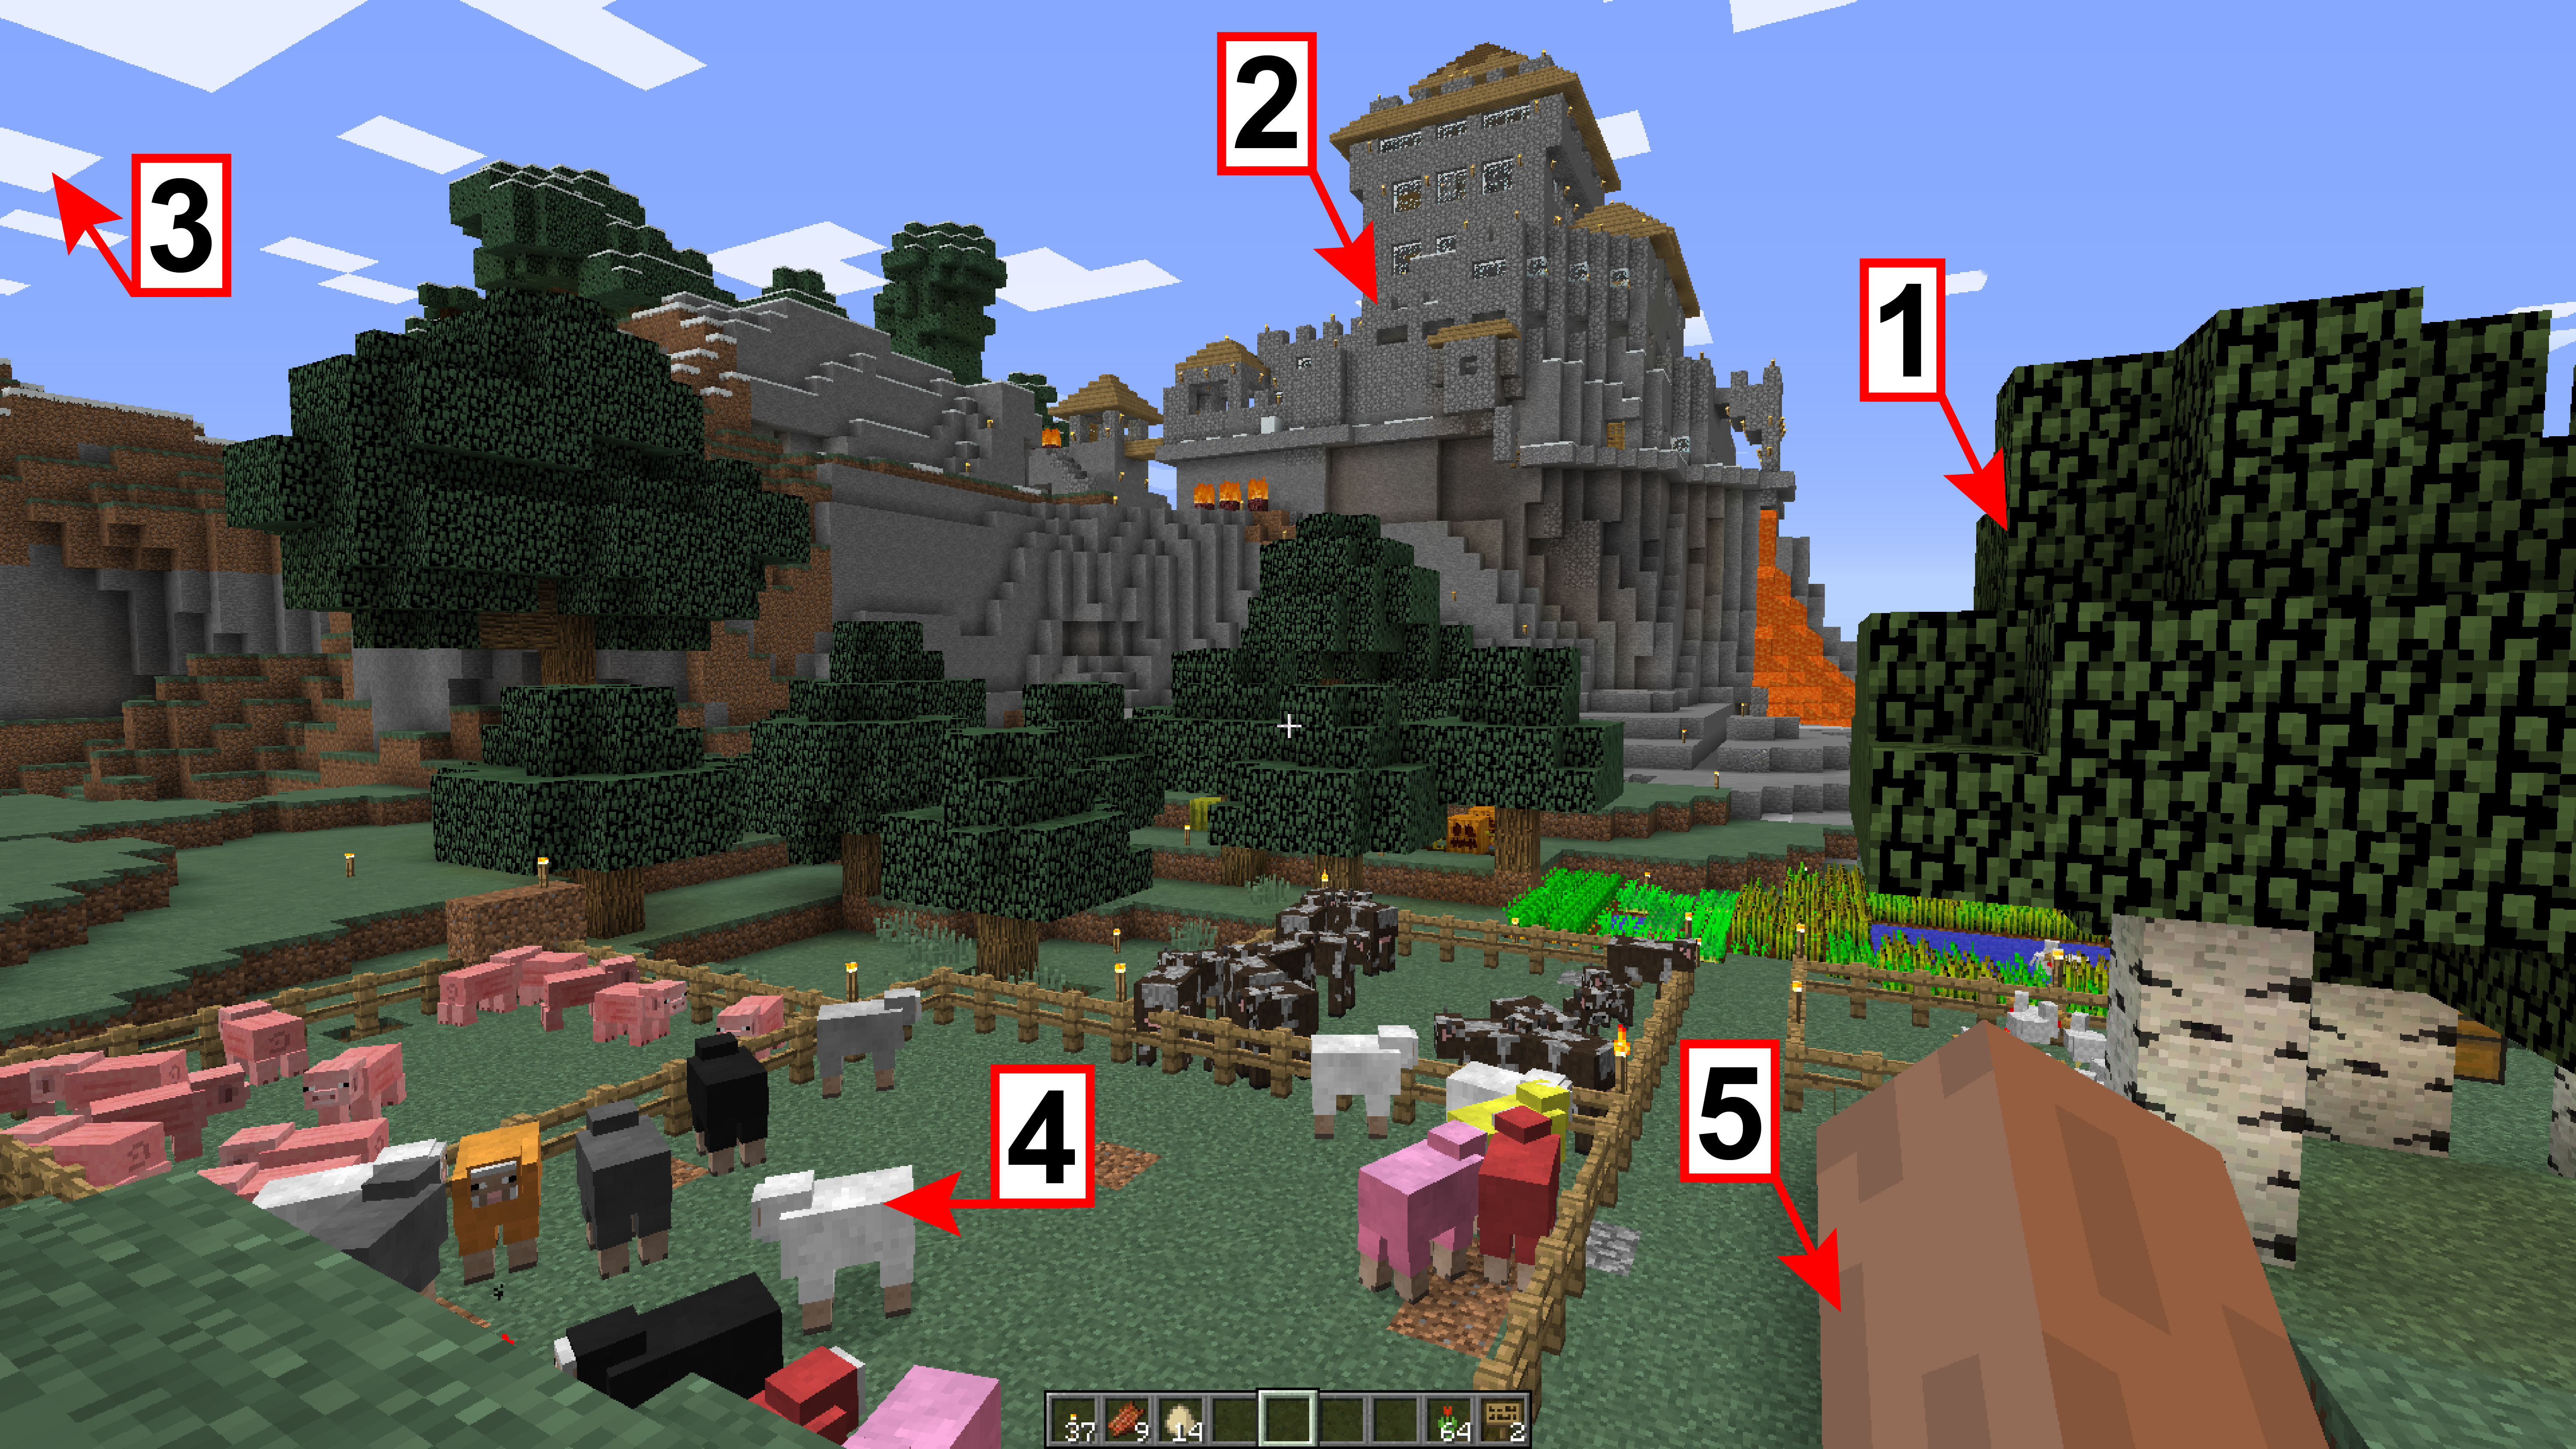
\includegraphics[ width=140mm]{../img/intro/mc}

\caption{Hra Minecraft - hrad na skále}
\label{fig:intro_mc}

\end{figure}

\FloatBarrier

Mezi dalšími hrami bychom mohli zmínit například \TE{}. Ta je o~něco mladší než \MC{}, ale je častým zdrojem diskusí, zda je lepší new \MC{}, nebo ne. Pravdou je, že obě hry mají svůj svět kompletně složený z~kostek (\TE{} je však 2D hra), ale každá si klade trochu jiné cíle. \TE{} je více orientovaná na příběh, obsahuje více \NPC{} i~bossů. Boss je v~herní terminologii významný nepřítel, obvykle je silnější než ostatní protivníci a~velmi často bývá v~závěrečných částech hry. Duel s~bossem pak obvykle od hráče vyžaduje zjištění jeho silných a~slabých stránek a~schémat jeho útoků \citep{intro_boss}. \MC{} je pak orientován spíše na stavění. (Porovnání Minecraft vs Terraria (facts) \citep{mc_te_comparsion} na Minecraftovém fóru.)


\subsection{Hry s~prvky realismu}

Mezi hry s~prvky realismu bychom mohli zařadit třeba hry \SE{} či \ME{}, využívají kombinaci herních bloků s~\textit{voxelovou} reprezentací světa. Obě hry jsou implementovány v~proprietárním enginu společnosti Keen Software House nazvaném \textit{VRAGE}\texttrademark{}. Voxelový terén je pak v~enginu za běhu hry procedurálně generován do polygonální reprezentace, kterou pak grafická karta standardním způsobem vykreslí na obrazovce (oficiální popis vlastností enginu \citep{vrage}). Během tohoto procedurálního vytváření je na třídimenzionální strukturu voxelů (které si můžeme představit jako bloky stejné velikosti) aplikován nějaký šum a~tím je možné ve hře vygenerovat prakticky neomezené množství různých objektů vycházejících z~jedné voxelové struktury. \uv{\textit{The “procedural asteroids” feature adds a~practically infinite number of asteroids to the game world}} \citep{rosa_blog}. Tímto způsobem pak hry dosáhují vyššího stupně realismu -- nespoléhají se pouze na předpřipravené 3D modely. 

Podívejme se na obrázek \ref{fig:intro_se} ze hry \SE{}. Na něm můžeme vidět převážně kamenný asteroid, a na něm je postavená vesmírná základna (obarvená zelenou barvou). K základně je přistavena větší vesmírná loď (modrobílá, v~levém horním rohu), hráč pak k~základně letí v~další, malé lodi (modrobílá uprostřed). Bližší pohled na planetku ukazuje, že její povrch není pravidelný. To je způsobeno právě algoritmickou aproximací voxelové reprezentace planetky. 

\begin{figure}[!ht]\centering
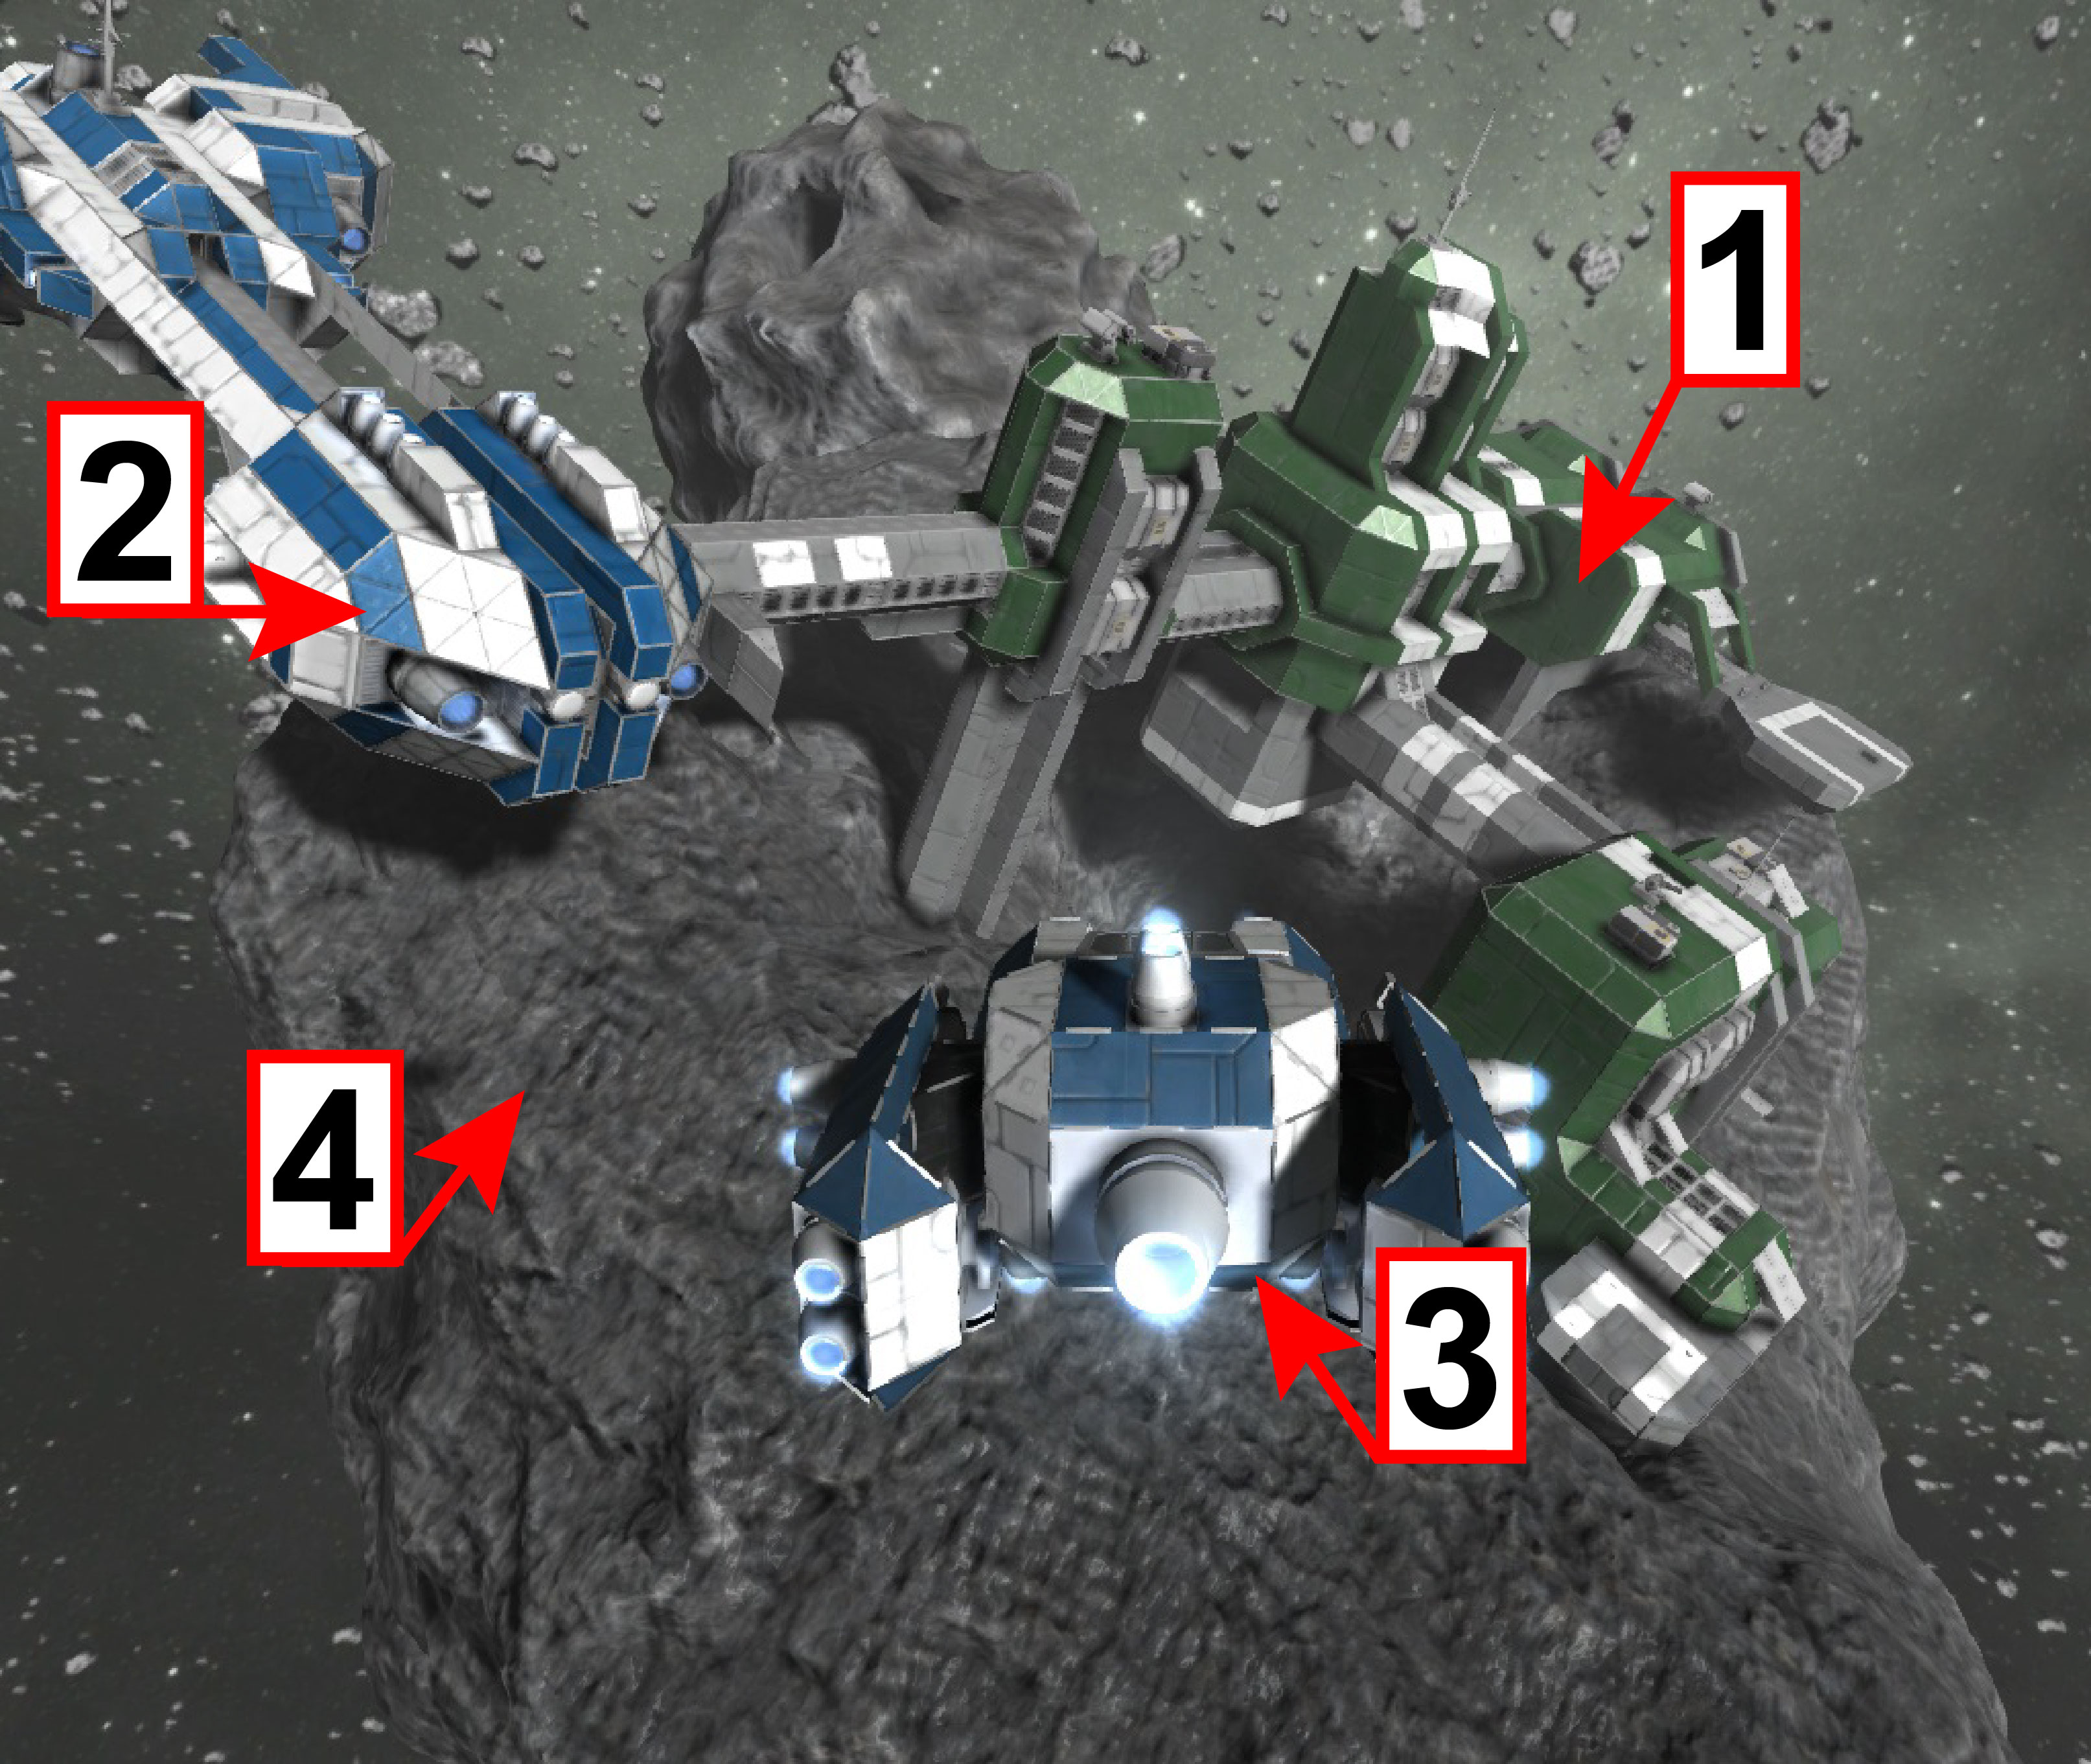
\includegraphics[ width=140mm]{../img/intro/se}

\caption{Hra Space Engineers -- základna. Zdroj: Gamespot.com \citep{se_intro_img} }
\label{fig:intro_se}

\end{figure}

\FloatBarrier

Samotná základna i~vesmírná plavidla (detailní pohled na jiné plavidlo je na obrázku \ref{fig:intro_se_ship}) jsou tvořeny bloky. Vizuální reprezentace bloku může být i~jiného tvaru než jen krychle -- to je možné vidět na obrázku \ref{fig:intro_se_blocks}). Barevně jsou zde zvýrazněny hranice bloků. Jak základny, tak vesmírné lodě (které jsou navíc oproti základnám pohyblivé) využívají tento systém. 

\SE{} umožňuje stavět pohyblivé stroje, které si hráč postaví z~herních bloků a~ty se pak chovají jako jedna entita. Stále je na ně však aplikována fyzika, takže je možné plavidlo poškodit, nebo dokonce zničit. Tento stupeň realismu od naší hry vyžadovat nebudeme. Budeme však chtít mít ve hře bloky, jejichž model není tvaru krychle. Stejně jako v \SE{} budeme chtít, aby bylo možné bloky rotovat v libovolném směru (u bloků, u kterých to bude dávat smysl).


TODO zmínit crafting, stavěnbí, conveyor systém

\begin{figure}[!ht]\centering
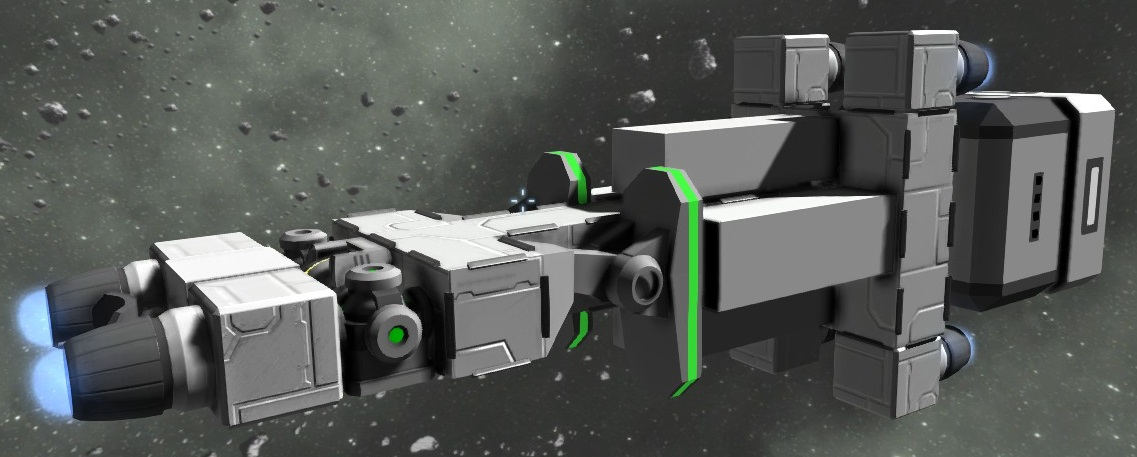
\includegraphics[ width=140mm]{../img/intro/se_ship}

\caption{Hra Space Engineers -- dron. Zdroj: space-engineer.net \citep{se_drone_source}}
\label{fig:intro_se_ship}

\end{figure}

\begin{figure}[!ht]\centering
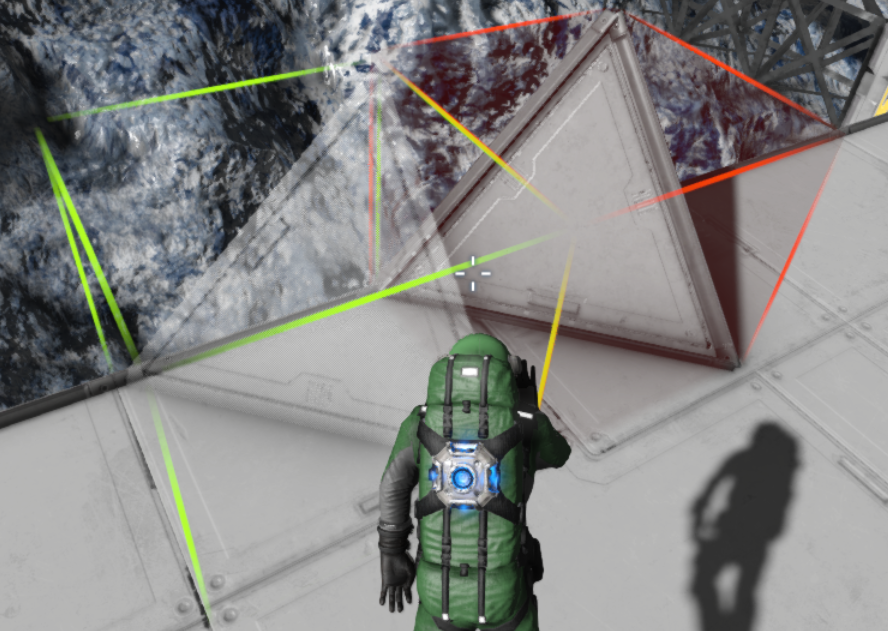
\includegraphics[ width=140mm]{../img/intro/se_blocks}

\caption{Hra Space Engineers - bloky }
\label{fig:intro_se_blocks}

\end{figure}

\FloatBarrier


\subsection{Hry s~maximálním důrazem na simulaci reality}

Do této sekce bychom měli zařadit například vesmírný simulátor \TM{}. // TODO popis, obrázek

Zmínit stavění

\begin{figure}[!ht]\centering
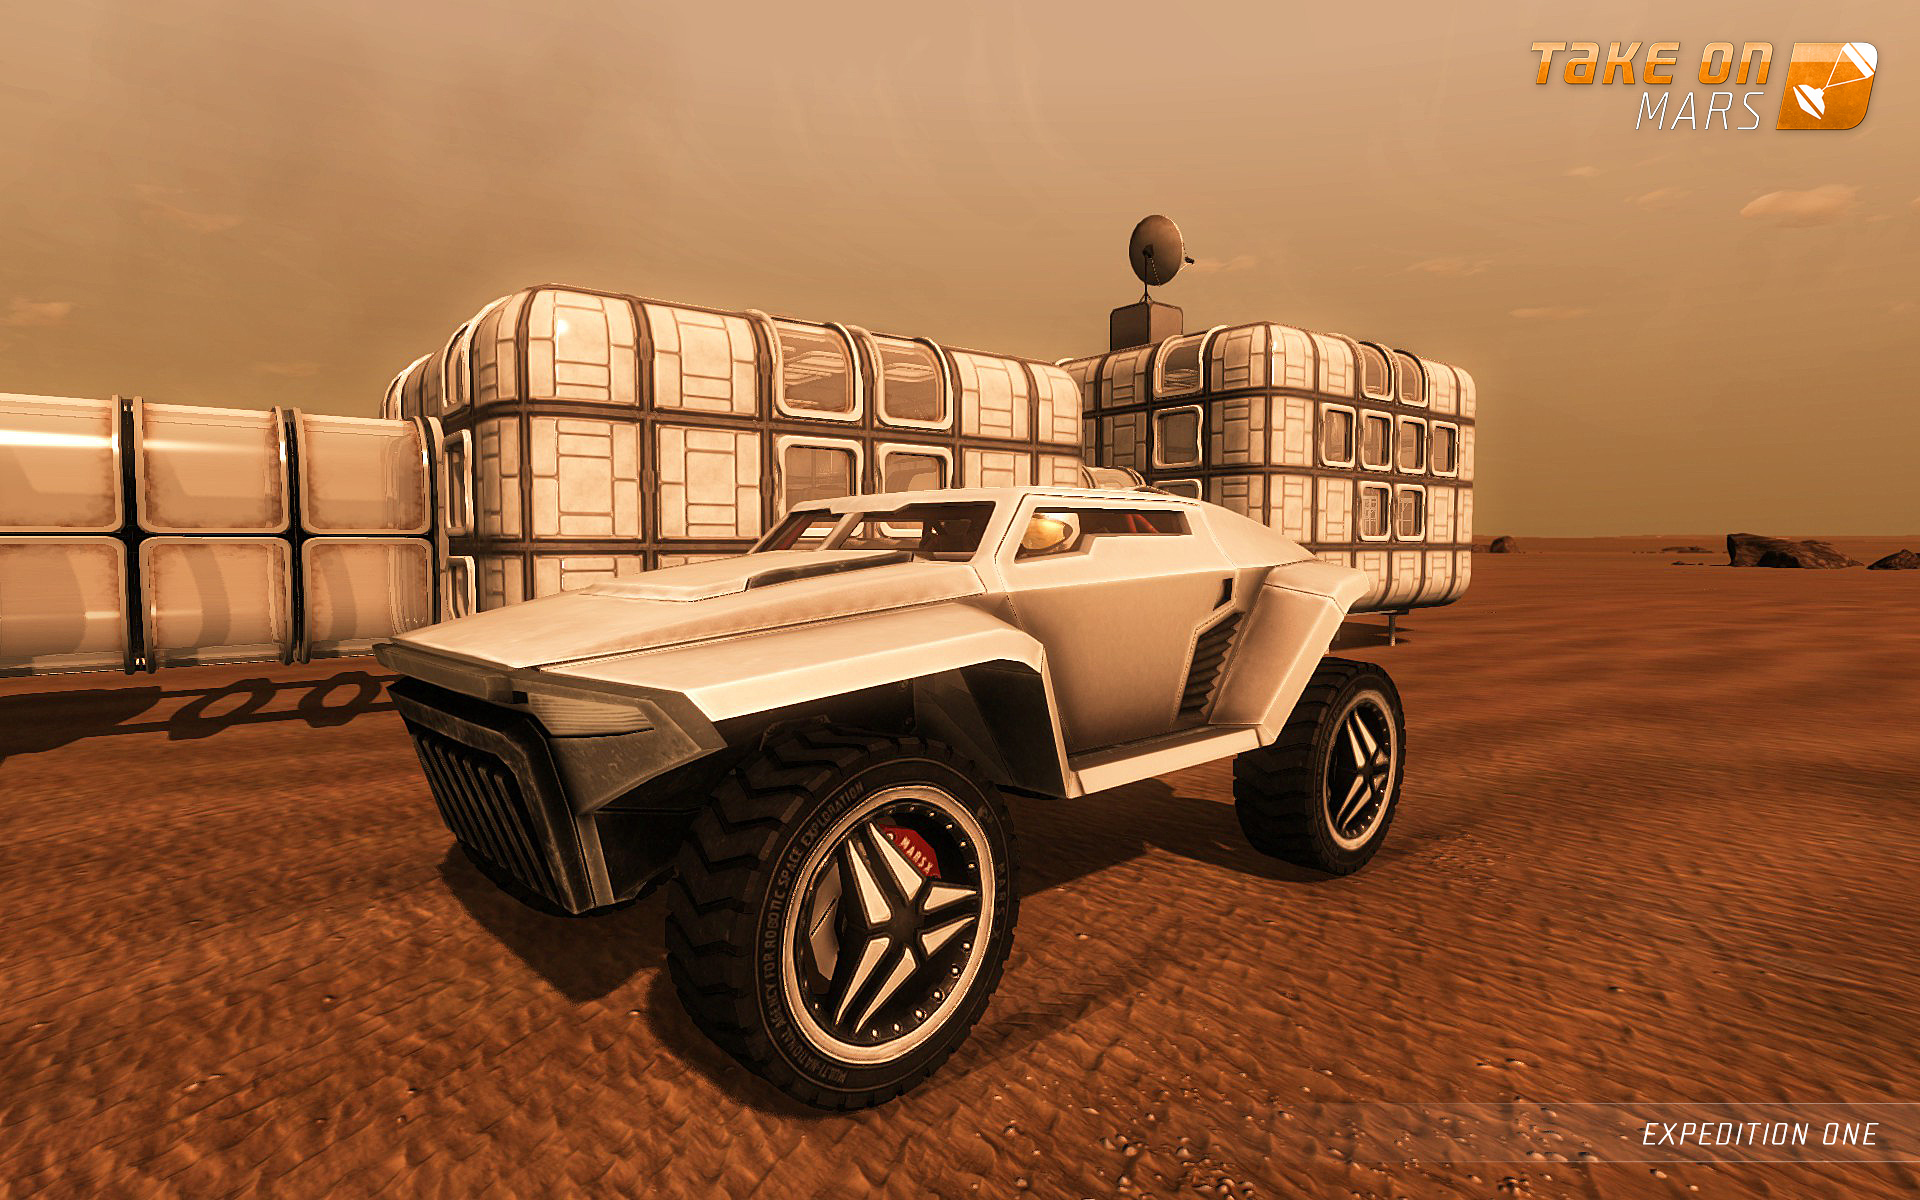
\includegraphics[ width=140mm]{../img/intro/tom}

\caption{Hry Take On Mars -- vozítko před budovou. Zdroj: Hry.cz \citep{intro_tom_source}}
\label{fig:intro_tom}

\end{figure}

\FloatBarrier

bloky na stavění, ale třeba vozidla kompletní

\subsection{Ostatní - zařadit TODO }

Můžeme však nalézt i~další příklady her (// TODO , , , , ).

\NI{}
Novus incpetio je MMORPG, stavění https://www.youtube.com/watch?v=d2ySkvn6wyw probíhá tím stylem, že se hráč přepne do build módu, vše si naplánuje (va výdledek vidí rovnou tak, jak bude vypadat). Po ukončení toho módu pak hráč vidí obrysy naplánovaných bloků. (Ty se přichytávají do mřížky a k sobě) Pak je může začít konstruovat, přičemž v nabídce během konstrukce má možnost si chybějící součásti craftnout.


\PN{}

https://www.youtube.com/watch?v=Wpurqr3YaGQ funguje podobně jako Space engineers - získávání surovin, kraftění na komponenty a použřívání komponent na konstrukci objetků. POstavený objekt ukazuje základní konstrukci.


\ARK{}
Ark počáteční free point, pak se bloky přidávají k sobě https://www.youtube.com/watch?v=TOmjjo5QoP8 


\NMS{}
Stejně jako \TM{} používá snappointy

\section{Čemu se budeme věnovat}

Rádi bychom zachovali koncept použití herních bloků, který shledáváme jednoduchý na pochopení i~použití. Zaměříme se na rozšíření možnosti práce s~bloky tak, abychom uživateli nabídli, pokud možno, ještě lepší herní zážitek ze stavění vlastních výtvorů. V této práci se nebudeme nijak důkladně věnovat vizuální reprezentaci prostředí, protože ta pro nás v~tuto chvíli není podstatná. 

Změna v~přístupu k~herním blokům bude vyžadovat i~úpravy herního mechanismu s~tím souvisejícího -- hráčova inventáře. Všechny výše zmíněné hry nějakým způsobem nabízí hráči výběr bloků, které může do herního světa umístit. Naše změna by bohužel znamenala, že by se takový inventář postavitelných bloků velmi rychle stal nepřehledným a~proto musíme systém nabídky postavitelných bloků upravit pro naše potřeby.

\section{Herní bloky}



Obvykle je ve hře definován jeden základní rozměr bloku, který je neměnný. (\SE{} definuje více velikostí -- ty však nelze vzájemně kombinovat). To však může být problémem, pokud se hráč rozhodne postavit v~herním světě nějakou větší a~komplexnější strukturu podle reálné či fiktivní předlohy. Pro příklad uveďme některé výtvory ze hry \MC{} -- město Královo přístaviště z~knih Píseň ledu a~ohně od Geoge R. R. Martina, nebo hlavní město Gondoru Minas Tirith z~knih Pána prstenů od J. R. R. Tolkiena.

Autoři těchto výtvorů museli volit takové měřítko, aby byly výtvory dostatečně detailní, ale zároveň aby bylo možné výtvor postavit v~nějakém rozumném čase. Obecně můžeme říct, že čím větších detailů chtějí autoři ve hře \MC{} dosáhnout, tím větší musí celý výtvor být. To pak ale znamená, že celá stavba trvá déle, nebo je zapotřebí více spolupracujících hráčů. Hra \SE{} díky svému přístupu a~více bloků, které nejsou tvaru krychle, nabízí lepší možnosti staveb rozsáhlých objektů (představme si třeba Hvězdu smrti z~Hvězných válek), ale stále je potřeba volit nějakou rozumnou výslednou velikost.


\subsection{Náš návrh úpravy}
Chtěli bychom se v~této práci zabývat myšlenkou proměnlivé velikosti stavitelných bloků. Tím by hráči mohli rychleji stavět rozsáhlejší struktury a~přitom se věnovat i~drobným či estetickým detailům. Tento návrh však s~sebou nese několik problémů, které se v~této práci budeme snažit vyřešit.


\section{Inventář}
Dalším společným prvkem tohoto druhu her je inventář bloků, které může hráč umístit do herního světa. Hráč přes celé herní okno vidí \HUD{} (Head-Up Display \citep{hud_terminology}), ve kterém má zobrazenou kromě jiného nabídku bloků, které má na rychlé volbě, může je snadno zvolit a~daný blok umístit do herního světa. Navíc hry mohou definovat i~inventární skupiny bloků (\SE{}, \ME{}), mezi kterými hráč může přepínat a~tím rychle kompletně změnit sadu rychlé nabídky. Vidíme však limitaci v~tom, že hráč musí ručně spravovat tyto seznamy a~jednotlivé bloky (či nástroje) umisťovat do příslušných pozic.


\subsection{Náš návrh úpravy}
Rádi bychom navrhli jiný způsob správy těchto inventárních skupin, aby hráč jednou definoval, jaké prvky chce mít v~příslušných skupinách. Při vytvoření nového bloku či vytvoření jiné velikosti bloku by pak nemusel ručně přiřazovat nový blok do skupiny, ale tento blok by měl být automaticky zařazen a~nabídnut hráči.  




\section{Cíle práce}
Tato práce by měla naplnit následující cíle:
\begin{itemize}
	\item Navrhnout a~implementovat způsob řešení proměnlivé velikosti bloků
	\item Navrhnout a~implementovat automatizovanou správu inventáře
	\item Kvůli očekávaným nárokům na pochopení nových konceptů do hry implementovat výukový tutoriál (TODO má to být tady?)
	\item Získat a~zhodnotit zpětnou vazbu na výslednou hru
\end{itemize}


%!TEX root = ../../prace.tex

\chapter{Analýza zadání}

V této části provedeme rozbor toho, jak různé hry v~současné době přistupují k~řešení jednotlivých součástí hry. Tím si připravíme prostor pro podrobnější specifikaci toho, jak by naše hra mohla vypadat a~co všechno by měla umět.

// TODO remove me:
Úkol zněl jasně: Cílem bakalářské práce je implementace budovatelské hry se strategickými prvky, hranou z~pohledu třetí osoby. Hra se odehrává na nehostinné planetě, kde je hráčův úhlavní nepřítel nedostatek zdrojů a~superkyselé deště. Hráč začíná v~menší budově – zbytek přistávacího modulu kosmické lodi. Dochází mu elektrická energie i~kyslík a~je na hráči, aby takticky využíval dostupné zdroje, hledal nové možnosti výroby energie a~přežil kyselé bouře. Cílem práce není vytvořit dohratelnou hru, spíše proof-of-concept, zda je tento typ hry s~uvedenými mechanikami zábavný a~má smysl v~jejím vývoji pokračovat i~nadále.

%!TEX root = ../../prace.tex


\section{Stávající implementace mechanismů}

Rozebereme si, jakým způsobem je v současné době přistupováno k blokům a jak jsou tyto bloky umisťovány do herního světa. Dále nás budou zajímat ostatní herní mechaniky, jako například denní cyklus, nebo jakým způsobem je řešena herní postava, její inventář a možnosti hráče interakce se světem. Poté se rozhodneme, jakým způsobem budeme uvedené mechaniky řešit my.

\subsection{Bloky}
\label{subsec:blocks}

Pod pojmem \uv{blok} budeme chápat objekt, který je umístěn v~nějaké ortogonální mřížce 3D prostoru a~beze zbytku tento prostor vyplňuje. Bloky spolu sdílí společnou množinu vlastností a dále pak samy definují své vlastní vlastnosti, které vychází z povahy bloku, tedy toho, co daný blok reprezentuje. V této kapitole rozebereme tyto vlastnosti a následně definujeme, jaké problémy budeme muset v této práci řešit.


\subsubsection{Základní vlastnosti}

Mezi základní vlastnosti bloku bychom měli zařadit \textit{vizuální reprezentaci}, \textit{pozici ve světě}, \textit{rotaci} a \textit{velikost}. Tento výčet není kompletní, ale můžeme říct, že jsou pro hráče nejvíce viditelné. Podle typu hry, jejího stylu a celkové koncepce bychom pak mohli do této množiny přidat třeba \textit{zdraví bloku}. V této části se zaměříme právě na základní vlastnosti a rozšiřujícím vlastnostem se budeme věnovat v následujících částech této kapitoly.

Vizuální reprezentace zřejmě vychází z povahy bloku. Vždy ale platí, že se vždy musí vejít do nějakých hranic bloku, obvykle daných v rámci pravidelné mřížky, ve které se blok nachází. Může v sobě zahrnovat i nějaké informace, které jsou pak hráčem vnímány pohledem. Kupříkladu mohou různými způsoby indikovat vnitřní stav objektu, podobně jako třeba svítivé diody indikují různé stavy elektronických zařízení v reálném světě. Podrobněji se budeme vzhledem zabývat až budeme řešit konkrétní bloky v naší hře.

Pozice bloku v herním světě je u her z kapitoly \ref{chap:uvod} může být buď na jednoznačně definovaném místě v herním světě, přičemž všechny bloky mají vůči sobě stejnou rotaci (\MC{}), nebo je blok součástí nějaké skupiny\footnote{Za skupinu budeme považovat shluk alespoň jednoho bloku a všechny bloky ve skupině musí být ve stejné mřížce.} bloků s jednoznačnou pozicí v herním světě. Tato skupina pak může mít libovolnou rotaci vůči nějakému globálnímu souřadnicovému systému a můžeme říct, že tato skupina tvoří lokální ortogonální systém. Různé skupiny mohou být vůči sobě různě natočeny. Toto chování je možné pozorovat třeba ve hře \ME{}, kde postavením prvního bloku určíme pozici a rotaci této skupiny. Pokud budeme chtít přidat do světa další blok, do nějaké vzdálenosti od prvního bloku je tento nově stavěný blok stále přichytáván do mřížky definované prvním blokem a rotace bloku jsou vždy o 90~stupňů. Obvykle platí, že první blok je umístěn vodorovně (tedy krychle bude i na šikmém terénu umístěna tak, že její horní a dolní strana je ve vodorovné poloze) a je možné ho libovolně rotovat kolem vertikální osy.

Rotace bloků jsou u naprosté většiny her řešeny v zásadě podobně. Výjimkou je pouze \MC{}, který rotaci bloků neumožňuje. U většiny bloků to nevadí, protože jsou bloky umístěny po směru, ze kterého je blok umisťován. Můžeme však nalézt některé speciality, třeba blok \textit{kolejí} (oficiální popis bloku \citep{mc_rail}). Koleje v \MC{u} mohou být rovné (ve směru sever -- jih nebo východ -- západ), mohou být nakloněné a překonávat výškový rozdíl mezi dvěma bloky, nebo mohou tvořit zatáčku. Díky absenci rotací tak hra používá několik pravidel, které určují výslednou podobu bloku. Podrobněji se jimi však zabývat nemusíme. U zbývajících her je situace, kterou jsme popsali v úvodu této části -- první blok je natočen vodorovně, má libovolnou rotaci dle vertikální osy a tímto určuje přichytávací mřížku pro další stavěné bloky.

Hry mají velikost bloků vždy stejně velkou. \MC{} má hranu bloku o~délce $1\,\rm m$ (popis bloku na oficiální Wiki stránce Minecraftu \citep{mc_block}, oficiální popis jednotek použitých v Minecraftu \citep{mc_units}). \SE{} sice bloky hranově omezuje dle kategorií od $0,5\,\rm m$ do $2,5\,\rm m$ (oficiální popis bloků ve hře \citep{se_blocks_wiki}), ale tyto kategorie mezi sebou nelze kombinovat a je možné k sobě vázat pouze bloky z jedné a té samé kategorie. U ostatních her je situace podobná, byť některé jsou v raných fázích vývoje a tudíž pro ně neexistuje žádný oficiální zdroj informací, takže velikosti bloků bychom mohli pouze odhadovat. 

Jako další základní vlastnosti bloku bychom mohli brát třeba \textit{zdraví}, \textit{cenu za postavení}, \textit{čas doby stavby}, \textit{délku trvání destrukce} (pokud vychází z hráčovy akce), co hráč získá za zničení bloku apod. U doby konstrukce a destrukce bloku můžeme říct, že doba trvání dané akce závisí na parametrech bloku a použitém nástroji. Kupříkladu v \MC{u} trvá kutání bloku kamene \textit{diamantovým} krumpáčem podstatně rychleji, než při použití krumpáče \textit{dřevěného}. Taktéž rychlost opotřebení nástrojů je různá. Nicméně když se ve hrách přepneme do tzv.~\textit{kreativního} módu, pak máme stavbu bloků \uv{zadarmo} a ihned. Tedy nemusíme mít žádné komponenty ke stavbě, ani specializovaný nástroj (případ \SE{}, \ME{}), nebo nám při postavení bloku tyto bloky neubývají z inventáře (\MC{}). 

\subsubsection{Součásti bloků}
Jako součásti bloků můžeme brát cokoliv, co rozšiřuje základní vlastnosti. Zde bychom mohli zmínit třeba \textit{Redstone} v \MC{u}. Redstone je speciální typ bloku, chová se jako elektrický vodič a v kombinaci s jinými bloky je možné vytvářet logická hradla. Je zřejmé, že pokud vhodným způsobem zkombinujeme určitá hradla, je možné v \MC{u} vytvořit třeba bitovou sčítačku. Ačkoliv vytvoření jednoho hradla je snadné, složitější logické obvody (například kódový zámek) jsou pak velmi náročné na prostor. Nejen z tohoto důvodu pro \MC{} vnikly různé módy, rozšiřující základní funkcionalitu hry o nové elektrické komponenty. Pro zajímavost, mód \textit{RedPower} (blog autora \citep{eloraam}) má jednotlivá hradla jako samostatné bloky (což šetří místo) a navíc má možnost skládat různě barevné vodiče (což jsou pouze ekvivalenty Redstonových bloků) do sebe (až 16~linek signálu). Bez tohoto módu by hráč potřeboval takový prostor, aby položil 16~vedení Redstone tak, aby se nedotýkaly a vzájemně neovlivňovaly (na rovině by tyto vodiče zabíraly šířku 31~bloků). 

Další možné součásti bloků, kromě vedení elektřiny, může být například práce s kyslíkem či práce s inventářem. Některé bloky hráči nabízí nějaký úložný prostor, kam může přesunovat objekty ze svého inventáře. Později pak hráč může k bloku přijít a objekty si opět navrátit do svého inventáře. Zajímavou specialitou je náhled inventáře. Kupříkladu u hry \ME{} se jedná stůl a~jídlo na stole. Stůl má svůj inventář, do kterého je možné umisťovat jídlo. Ve hře je pak obsah inventáře stolu zobrazen tak, že jídlo má svůj náhledový model na talířích na stole, takže to vypadá, jako by bylo jídlo připraveno ke konzumaci. 


Dále můžeme zmínit interakci s uživatelem, ať už přímou, nebo nepřímou. Jako přímou interakci budeme chápat takové použití bloku, kdy rovnou vidíme nějakou změnu. To může být například stisknutí tlačítka, nebo změna polohy nějaké páky. Výsledek této přímé interakce pak hráč vidí okamžitě a vizuálně se blok nějakým způsobem změní. Jako nepřímou interakci bychom mohli uvést například otevření nějakého ovládacího rozhraní bloku, což je obvykle nějaká UI obrazovka. Obě interakce se mohou prolínat, takže výsledkem nepřímé interakce může být třeba změna barvy bloku.


\subsection{Komunikace bloků}
Bloky spolu mnohdy umí komunikovat. Dříve zmíněný Redstone z \MC{u} by se dal taktéž považovat za jistou metodu komunikace mezi bloky. Například stiskem tlačítka lze změnit výstupní Redstonový signál z tohoto tlačítka (třeba z neaktivního na aktivní), který způsobí změnu polohy nějakého pístu. Ovšem komunikace může být i méně viditelná -- například z terminálu v \SE{} je možné ovládat písty, otevírat a zavírat dveře hangáru apod. bez explicitních vodičů signálu.

Ve hrách \MC{} a \SE{} můžeme nalézt příklad dopravníkových systémů. Ty umožňují \uv{poslat} bloky či objekty na jiné místo, kupříkladu z jednoho křídla budovy do druhého. V \MC{u} bez módů se této funkcionality dá vcelku snadno dosáhnout, nicméně je to zdlouhavé a rychlost přesunu bloků je poměrně pomalá. Ale opět se můžeme obrátit na módy, třeba na \textit{BuildCraft} (oficiální stránky projektu \citep{buildcraft}), který umožňuje rychle dopravovat bloky i na velké vzdálenosti. Hra \SE{} má kvalitní dopravníkový systém už ve svém základu a slouží například pro dopravu natěženého materiálu od bloku \textit{Vrtáku} do bloku \textit{Skladiště} (který má svůj inventář). Svým způsobem je pak přeprava v rámci těchto systémů také druhem meziblokové komunikace - bloky si mezi sebou předávají konkrétní instance objektů.

\subsection{Skládání bloků do struktur}
Asi jediné příklady, který můžeme zmínit, jsou ve hře \MC{} -- postavení portálu do Netheru (obrázek \ref{fig:structs_nether_portal}), sněhuláka či golema. V momentě, kdy nějaká skupina bloků splňuje přesně definovaný tvar, tak se tyto bloky chápou jako jedna struktura a tak se s nimi i zachází. Portál je možné pomocí \textit{křesadla} aktivovat, ale pokud je portál aktivní a hráč odebere z portálu některý blok, který jej tvoří, portál se uzavře. Bloky ve tvaru sněhuláka a golema se po dokončení tvaru odeberou a namísto nich je do světa umístěno \NPC{} sněhuláka či golema.

\begin{figure}[!ht]\centering
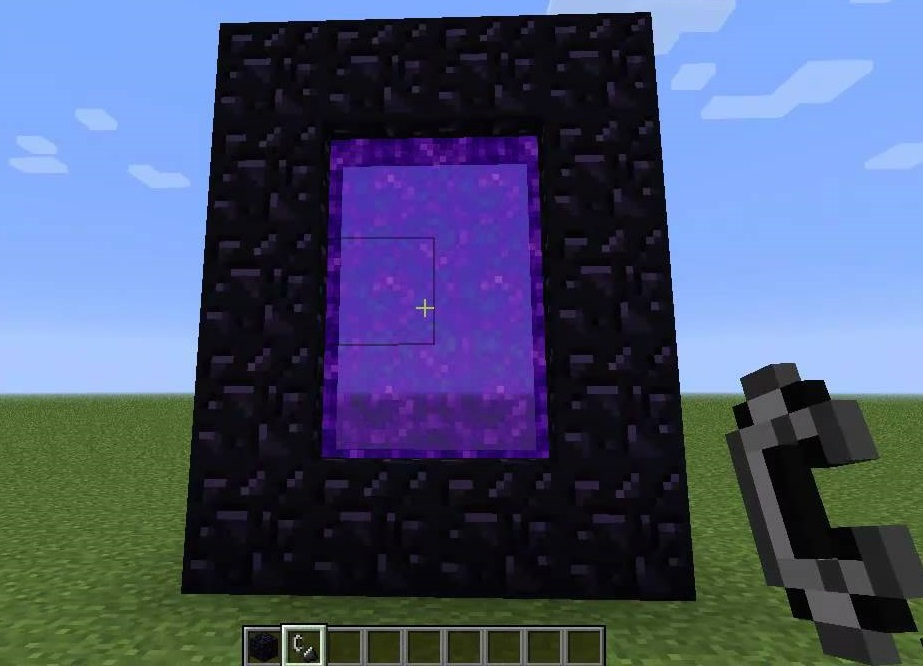
\includegraphics[ width=140mm]{../img/analysis/mc_portal}

\caption{Portál do Netheru. Zdroj: minecraftpocketedition.wikia.com \citep{mc_nether_portal}}
\label{fig:structs_nether_portal}

\end{figure}

\FloatBarrier



\subsubsection{Speciality}
Ve hrách \ME{} a  \NMS{} můžeme nalézt zajímavou funkcionalitu \textit{multibloků}. Tato funkcionalita nabízí například nahrazení nějaké stěny nějakého bloku oknem či nějakým dalším vizuálním či funkčním elementem.


Také bychom měli zmínit propagaci kyslíku v rámci postavených budov, kterou můžeme nalézt ve hrách \SE{} nebo \TM{}. Ačkoliv tento koncept je spíše vlastností herního prostředí, velice úzce souvisí s bloky. Pokud bloky tvoří uzavřenou strukturu, tak je možné vnitřní prostory natlakovat, zaplnit kyslíkem a sundat si helmu či dokonce celý skafandr. \SE{} využívá systém tzv.~\uv{místností} (oficiální dokumentace o kyslíku \citep{se_oxygen}). Místnosti lze zaplnit kyslíkem díky \textit{ventilaci}, což je blok, který umí do prostoru místnosti vhánět kyslík a také ho z něj odebírat. \TM{} dělá prakticky to samé, liší se pouze způsobem implementace rozpoznání místnosti, což souvisí se způsobem stavby bloků (jak jsme zmínili v kapitole \ref{chap:uvod}).


\subsection{Herní svět}

V této části se zaměříme na zpracování herního světa a s tím souvisejících mechanik.

\subsubsection{Reprezentace}

Pokud shrneme poznatky z kapitoly \ref{chap:uvod}, tak můžeme říct, že máme v zásadě dvě možnosti. Buď můžeme po vzoru \MC{} mít celý svět tvořen bloky. Pak bychom kvůli optimalizaci výkonu také museli tyto bloky shlukovat do skupin (v \MC{u} se jim říká \textit{chunks} a jsou velké $16*16*256$ bloků). Nebo můžeme mít po vzoru \SE{} svět více realistický -- a třeba po vzoru této hry hráči připravit třeba celé planety (oficiální představení přidání planet do hry \citep{se_planets}). Koncept planet se objevuje i v dalších hrách (\ME{}, \NMS{}, atd.).

\subsubsection{Bloky v~herním světě}

Jak jsme se zmínili v části \ref{subsec:blocks}, bloky jsou v herním světě umístěny vždy do nějaké mřížky. Různé hry však nabízí různé možnosti práce s těmito mřížkami a ta navíc vychází z možností reprezentace herního světa.


\subsubsection{Denní / noční cyklus}

Všimněme si, že všechny hry implementují denní cyklus. To dodává hře na dynamičnosti -- ne všechny hráče by bavilo desítky či stovky hodin trávit v identickém prostředí. Navíc, pro vývojáře je to možnost, jak hráči připravit nějaké nebezpečí spojené s příchodem noci. Jeden příklad za všechny -- v \MC{u} se mnozí nepřátelé začínají objevovat, až když je pro ně dostatečná tma. Což nemusí být nutně způsobeno začátkem noci, stačí třeba málo osvětlená jeskyně ve skále či podzemní prostory. Ovšem denním cyklem je hráč nucen se nepřátelům bránit a tím je pro něj zajištěn nějaký netriviální herní prvek, po jehož překonání má hráč obvykle radost a pocit úspěchu.
Délka denního cyklu se různí podle hry. \MC{} má délku dne 20 minut, u dalších her to bude podobné.


\subsubsection{Herní překážky}

Mezi další herní překážky bychom mohli zařadit třeba \textit{proměnlivé počasí}, přítomnost nepřátelských \NPC{} nebo různá omezení herní postavy, za kterou hráč hraje. Mezi to se může počítat třeba \textit{zdraví}, \textit{výdrž}, \textit{hlad}, zbývající \textit{zásoba kyslíku} či \textit{energie} a mnohé další. Všechny námi zmiňované hry tyto mechanismy implementují a výsledný dojem z nich není u žádné z her natolik zásadní a inovativní, abychom se tím hlouběji zabývali.

\subsubsection{(Ne)fyzikální chování}

Za zmínku stojí také přítomnost fyziky ve hře. Hry s vyšším či úplným stupněm realismu ji implementují a u každé hry se více či méně přibližuje realitě. Vymyká se hra \MC{}, jejíž fyzikální model se může zdát na první pohled zvláštní, ale je zapotřebí si uvědomit, že tento model zapadá do celkové koncepce hry. Proto je v této hře poměrně zajímavá mechanika kapalin, která je zcela nefyzikální a umožňuje vytvoření nekonečných zdrojů vody. Ostatně sám blok zdroje vody je možné umístit z boku k nějakému sloupu a voda bude neustále vytékat. Pokud navíc odebereme bloky ze sloupu, voda bude vytékat z ničeho a bude z daného místa vytékat dokud dané místo nenahradíme nějakým pevným blokem, třeba hlínou či pískem. Stejně jako voda se ve hře chová i láva, její chování se liší v drobných detailech (například se šíří pomaleji než voda).

Další zajímavou vlastností je \uv{levitace} bloků. Trochu jsme na toto chování narazili v předcházejícím odstavci, tak to rozveďme. Každý blok obývá právě jednu pozici v herním světě. A u většiny bloků platí, že mohou zůstat viset volně ve vzduchu. Ale například u \textit{písku} se po přidání nebo odebrání některého z okolních bloků provede aktualizace bloku. A když takový blok zjistí, že by neměl být jen tak ve vzduchu (pod ním nic není), tak začne padat dolů. A jak nastane situace, že hráč potká ve vzduchu visící písek? To souvisí s algoritmem generování, který má více cyklů a ve výsledku mohou být v herním světě umístěny obdobné kuriozity. Nicméně stačí jeden přidaný či odebraný blok v těsné blízkosti a bloky se začnou kaskádovitě sypat dolů. Tam se opět úhledně seskládají do sloupců (i když jsou to třeba bloky písku, které by se v reálném životě sesypaly na hromadu).


\subsection{Inventář}
\label{subsec:inventory}

Obdobně jako u fyziky ve hrách, chování inventáře je závislé na stupni realismu. \MC{} nabízí 27 slotů inventáře, 9 slotů rychlé nabídky a 4 sloty pro brnění. Sloty inventáře a rychlé nabídky jsou plněny \textit{kupitelnými předměty}. To znamená, že podle typu bloku či předmětu může být v daném slotu 1 až 64 prvků daného objektu. Takže například je možné mít v jednom slotu 64 kusů \textit{hlíny}, ale jen 16 kusů \textit{vajec} a pouze 1 \textit{meč}. Plnění rychlé nabídky je možné z UI nabídky inventáře pomocí systému Drag and Drop. Navíc za použití kláves Ctrl a Shift lze řídit počet přenášených kusů daného objektu. Při stavění se blok z daného rychlého slotu odebere, zbraň či nástroj se opotřebí.

U \ME{} a \SE{} jsou také pevné sloty, ale existuje zde koncept \textit{skupin slotů}. Přepínáním těchto skupin se mění všechny sloty rychlé nabídky, takže je možné si do různých skupin nastavit různé stavební prvky. Můžeme říct, že \MC{} má pouze jednu skupinu slotů. V momentě, kdy hráč staví z více prvků než je velikost rychlé nabídky, se tato funkcionalita stává potřebnou, aby hráč nemusel neustále přehazovat stavěné bloky. Výhodou je, že u těchto her jsou bloky spíše konstrukčního charakteru a neodebírají se z inventáře, takže prvky ve skupině slotů zůstávají zachovány. V \MC{u} by i při této funkcionalitě bylo potřeba udržovat skupiny slotů, protože jak jsme již zmínili, stavba v této hře odebírá položky z inventáře.

Co se týče stavění, zbývající hry nepřináší nic nového či převratného. Pozorný čtenář si mohl všimnout, že v \MC{u} je možné, aby hráč nesl $36*64$ kostek kamene, každou o objemu $1\,\rm m^3$. Je zřejmé, že nosnost opět nevychází z realistických předpokladů. Nicméně u her s vyšším stupněm realismu se u nosnosti setkáváme, takže kupříkladu je omezena váha, kterou může hráčova postava nést. Navíc se u některých her s rostoucí zátěží zpomaluje pohyb. I toto je součástí herního designu, který větší či menší měrou odráží fyzikální realitu.

\subsection{Herní postava}
Mezi vlastnosti herní postavy bychom mohli zmínit \textit{zdraví}, \textit{výdrž}, \textit{hlad} a další podobné charakteristiky. Tyto vlastnosti jsou vlastně \textit{survival} prvky a hráč se musí o svoji herní postavu \uv{starat}, aby mu neumřela a bylo možné hru hrát dál. Zde opět můžeme říct, že tyto herní mechaniky hry z kapitoly \ref{chap:uvod} implementují podobným způsobem.
Další vlastností, kterou jsme již zmínili, je nosnost v rámci inventáře postavy. Podrobněji jsme tuto mechaniku rozebrali v části \ref{subsec:inventory} a proto se tím zde nebudeme podrobněji zabývat. 
Dále bychom mohli zmínit možnost přepínání pohledů (pohled z 1. osoby nebo z 3. osoby), což většina her také má. 




%!TEX root = ../../prace.tex



\section{Co bychom chtěli implementovat}

V následujících podkapitolách si rozebereme naše požadavky na hru



%!TEX root = ../../prace.tex

\subsection{Bloky}

TODO  Většina bloků je stejně velká a má hranu o délce 1 metru \citep{mc_block}, \citep{mc_units}. (TODO přesunout do detailní analýzy. TODO popisek odkazu)

V současné době jsou velikosti bloků omezeny na konstantné velikost. Ve hře Minecraft je blok hranově omezen na 1m, hra Space Engineers bloky omezuje dle kategorií od 0.5\,\rm m do 2.5\,\rm m \citep{se_blocks_wiki}.


různé druhy, velikosti, jejich vizuální reprezentace, rozšiřovatelnost, obecně co všechno by měly umět.

Název - Min - Max - Pitch - Roll - Type (kostka, zkosený, roh, vlastní)

Tam kde Min == Max -> Vlastní škálování

Typ ovlivňuje další chování

Třeba u Světla by typ mohl být i K a hra by se chovala stejně, K = 1, Z = 0.5, R = 1/6, V = 1 (není v potaz objem)

komponenty bloků a nějaké další ptákoviny

\begin{tabular}{|rll*{5}{c}|}
	\hline
	\tableColumnTitles{Název}								{	&	Min		&	Max			&	P			&	R			&T	}		\hline
	\currentCategory{\textbf{Základní bloky}} 																					\\		\hline
		\mytablerow 				& Blok základny				& 1--1--4	& 20--20--4		& 				& 				&K	\\		\hline
		\mytablerow 				& Blok stavby				& 1--1--1	& 20--20--20	& \checkmark	& \checkmark	&K	\\		\hline
		\mytablerow 				& Blok polykarbonátu		& 1--1--1	& 20--20--20	& \checkmark	& \checkmark	&K	\\		\hline
		\mytablerow 				& Zkosený blok základny		& 1--1--4	& 20--20--4		& 				& 				&Z	\\		\hline
		\mytablerow 				& Zkosený blok stavby		& 1--1--1	& 20--20--20	& \checkmark	& \checkmark	&Z	\\		\hline
		\mytablerow 				& Roh bloku stavby			& 1--1--1	& 20--20--20	& \checkmark	& \checkmark	&R	\\		\hline
	\currentCategory{\textbf{Speciální bloky}} 									 												\\		\hline
		\mytablerow 				& Terminál			 		& 1--8--5 	& 1--8--5		& 				& 				&V	\\		\hline
		\mytablerow 				& Napájené okno				& 2--1--2	& 20--1--20		& \checkmark	& \checkmark	&K	\\		\hline
		\mytablerow 				& Dveře 					& 7--7--11	& 7--7--11		& 				& 				&V	\\		\hline
		\mytablerow 				& Světlo					& 1--1--1	& 1--1--1		& \checkmark	& \checkmark	&V	\\		\hline
		\mytablerow 				& Přepínač 					& 1--1--1	& 1--1--1		& \checkmark	& \checkmark	&V	\\		\hline
		\mytablerow 				& Generátor energie			& 3--3--2	& 20--20--2		& 				& 				&K	\\		\hline
		\mytablerow 				& Generátor objektů 		& 3--3--2	& 20--20--2		& 				& 				&K	\\		\hline
		\mytablerow 				& Akumulátor				& 3--3--3	& 3--3--3		& 				& 				&V	\\		\hline
		\mytablerow 				& Plnička kyslíkových bomb 	& 4--3--4	& 4--3--4		& 				& 				&V	\\		\hline
		\mytablerow 				& Kyslíková bomba			& 2--2--2	& 2--2--2		& 				& 				&V	\\		\hline
		
\end{tabular}


\subsection{Podrobný popis bloků}

Popis některých vlastností - má energetickou komponentu - > implikuje definici bindovacích bodů
má kyslíkovou komponentu - implikuje TotalObjectOxygen

Producer nebo Consumer implikuje Total object energy

Controllable implikuje IsController nebo IsControllable



\subsubsection{A1 - Blok základny}
- velikost v ose Z omezena na 4 základní bloky

- má elektriku

Pokud bychom měli nerovný terén, tento blok by mohl zahrnovat podstavce pro vyrovnání terénu.

\subsubsection{A2 - Blok stavby}
- všechny velikosti

- má elektriku

Tento blok je základním stavebním blokem ve hře.

\subsubsection{A3 - Blok polykarbonátu}
- všechny velikosti
Tento blok je nejlevnější, není připojen do elektrické sítě. Ideou bloku je podpora průhledných stěn a také možné pomocné stavební konstrukce pro výstavbu do výšky. Inspiraci můžeme vidět v používání třeba bloku hlíny ve hře \MC{}, kdy hráč vyskočí a pod sebe umístí nový blok a tím se ve světě posune o 1 metr výš.

\subsubsection{A4 - Zkosený blok základny}
- velikost v ose Z omezena na 4 základní bloky

- má elektriku

Stejné jako blok \textit{A1}, jen je zkosený. Může sloužit jako přístupová rampa.

\subsubsection{A5 - Zkosený blok stavby}
- všechny velikosti

- má elektriku
\subsubsection{A6 - Roh bloku stavby}
-všechny velikosti

- má elektriku

\subsubsection{B1 - Terminál}
- speciální, pevná velikost 1 x 8 x 5 bloků

- má elektriku, konzument, rychlé doplnění energie, ovládání rozhraní, komplexní přehled připojené elektrické sítě.
\subsubsection{B2 - Napájené okno}
- minimální velikost 2 x 1 x 2, maximální velikost 20 x 1 x 20 základních bloků

- má elektriku, konzument
\subsubsection{B3 - Dveře}
- speciální, pevná velikost 7 x 7 x 11 bloků

- má elektriku, otevírání
\subsubsection{B4 - Světlo}
-velikost omezena na 1 x 1 x 1 blok

- má elektriku, konzument, ovládání bez přepínače
\subsubsection{B5 - Přepínač}
-velikost omezena na 1 x 1 x 1 blok

- má elektriku, náhled stavu
\subsubsection{B6 - Generátor energie}
- omezená velikost v ose Z na 2 bloky, jinak 3 x 3 až 20 x 20 v ostatních osách

- má elektriku, producent
\subsubsection{B7 - Generátor objektů}
- omezená velikost v ose Z na 2 bloky, jinak 3 x 3 až 20 x 20 v ostatních osách

- má elektriku, konzument
\subsubsection{B8 - Akumulátor}
- speciální, pevná velikost 3 x 3 x 3 bloků

- má elektriku, producent, konzument, rychlý náhled naplnění
\subsubsection{B9 - Plnička kyslíkových bomb}
- speciální, pevná velikost 4 x 3 x 4 bloků

- má elektriku, kyslíkovou komponentu, konzument, UI, rychlé doplnění kyslíku

- využijeme ideu náhledu inventáře a plnička bude zobrazovat blok B10, pokud bude nějaký takový blok plnit.

\subsubsection{B10 - Kyslíková bomba}
- speciální, pevná velikost 2 x 2 x 2 bloků

- má kyslíkovou komponentu, možnost sebrat, rychlý náhled naplnění, rychlé doplnění kyslíku







\subsection{Herní svět}

jaký chceme herní svět

\subsubsection{Reprezentace}

bude nám stačit nějaký tree, definovat rozměry, na chuncky kašlem

\subsubsection{Bloky v herním světě}

do gridu

\subsubsection{Denní / noční cyklus}
dáme ho

\subsubsection{Herní překážky}

počasí, , atributy avataru

\subsubsection{(Ne)fyzikální chování}

nebudeme hrotit

\subsection{Inventář}

chceme volné sloty, rozšiřitelnost

\subsection{Avatar hráče}
avatar má nějaké vlastnosti, \HUD{}, 1St / 3rd person view, zdraví, O2, energie







\section{Herní nepřítel}
Protože samotné stavění bez nějakého cíle či překážky není úplně zábavné, musíme hráči připravit nějakou překážku, komplikaci, kterou musí překonávat. Zde neexistuje jednoznačné řešení --- to je závislé na celkovém prostředí hry, zamýšlené cílově skupině a~mnoha dalších faktorech. Cílem našeho hráče bude přežít kyselé deště. Ty budou přicházet v~náhodných intervalech a~budou sloužit jako překážka v~rozvoji hry. Zároveň to ale bude pro hráče nástroj, jak získávat prostředky pro ochranu před dalšími dešti a~rozvoj svých staveb. 

\section{Backlog}


???




TODO Tento stupeň realismu od naší hry vyžadovat nebudeme. V naší hře ale budeme chtít mít bloky, jejichž model není tvaru krychle. Stejně jako v \SE{} budeme chtít, aby bylo možné bloky rotovat v libovolném směru (u bloků, u kterých to bude dávat smysl).

TODO Pokud bychom se rozhodli řešit vnitřní prostory stavěných budov a jejich plnění kyslíkem, tak bychom se z tohoto stylu mohli inspirovat.

Touto myšlenkou bychom se chtěli inspirovat.  (TODO Pozn. opravdu? když jsem vymyslel konstruktor objektů, tak jsem TOM ani nehrál)
%!TEX root = ../prace.tex

\chapter{Detailní analýza}

V této kapitole podrobně rozebereme cíle práce. Už víme, čeho bychom chtěli dosáhnout a nyní potřebujeme vyřešit \textit{jak} toho dosáhnout.

%!TEX root = ../prace.tex

\section{Použitý herní engine}
- máme několik možností:

- napsat si vlastní (ne, moc práce)

- použít low level (XNA) - opět ne, moc práce

- Unity nebo Unreal Engine

- Unity mělo alespoň v době analýzy této práce problémy s dynamickým navmeshem, oproti tomu mělo editovatelný terén. Další nevýhoda je absance editorů materiálu tk jak je tomu v UE

- Unreal je prostě nej

%!TEX root = ../../prace.tex

\section{Bloky}

V této části rozebereme, jak můžeme definovat a~následně implementovat bloky a~popíšeme, jaké jsou výhody a~nevýhody jednotlivých implementací.\linebreak V~prvé řadě se zaměříme na celkovou strukturu bloků a~následně budeme řešit, jak budeme spravovat konstanty ovlivňující chování bloků.

\subsection{Celková struktura}

Aby se nám s~bloky dobře pracovalo, jistě bude vhodné využít jednoho ze základních principů \textit{OOP} (objektově orientovaného programování) -- dědičnosti. Takže v~naší hře bude existovat základní třída, která bude vycházet ze třídy \TT{UActor}\footnote{\TT{UActor} je základní třída \UEu{}, ze které dědí všechny herní objekty, které chceme v~hlavní herní smyčce aktualizovat a~renderovat.} a~bude předkem všech našich herních bloků. Tato třída by měla být kvůli rychlosti napsána v~\CPP{}.

Tento prapředek bude obsahovat dvě podstatné informace -- referenci na \textit{definici} daného bloku a~referenci na třídu s~vlastnostmi dané \textit{instance} bloku. Díky tomu, že oddělíme definiční třídu a~instanční třídu, tak získáme možnost získat definiční třídu pro daný typ bloku za běhu hry pouze jednou a~posléze tuto referenci předávat všem instancím bloku daného typu. Instanční třída bude mít pro každý blok jiné hodnoty, takže je zřejmé, že by měla být samostatná. Smyslem definičního souboru je popis omezujících podmínek kladených na daný typ bloku (například povolené minimální a~maximální rozměry), přičemž hodnoty v~instanční třídě by měly být v~mezích dané definicí. Vlastnosti, které nejsou omezující (například cena za postavení bloku), nebudeme uchovávat v~\textit{instanční} třídě, tyto údaje budeme získávat přímo z~\textit{definiční} třídy.

Pokud bychom zvolili jiný postup, snadno bychom si mohli \uv{svázat} ruce. Pokud by například \textit{instanční} vlastnosti byly vlastní součástí bázové třídy, systém ukládání hry by musel být schopen vidět a~pracovat minimálně s~touto bázovou třídou. Pokud však tyto vlastnosti vložíme do nějakého kontejneru (tedy třídy, která bude sloužit pouze jako přepravka pro data), tento kontejner klidně můžeme umístit do samostatného modulu\footnote{Moduly si lze představit jako samostatné knihovny, které se navzájem (acyklicky) referencují.}, nezávisle na modulu bloků a~modulu ukládání hry. Podrobněji se herním modulům věnujeme v~části \ref{sec:struct}.

\subsection{Instanční vlastnosti}
\label{subsec:instVlast}
Mezi instanční vlastnosti zařadíme vlastnosti definované v~části \ref{subsec:blocks} -- \textit{vizuální reprezentaci}, \textit{pozici ve světě}, \textit{rotaci}, \textit{velikost}, \textit{zdraví} apod. U~některých vlastností bychom navíc chtěli dosáhnout toho, aby konkrétní instance bloků měly rozdílné hodnoty dané vlastnosti v~závislosti na jejich velikosti. Jako ideu si můžeme představit následující: blok, který je větší než jiný blok stejného typu, bude mít více zdraví, protože je bytelnější a~více toho vydrží. Z~této úvahy nám zároveň vyplývá, že kromě rozměrů bloku se do výpočtu zapojuje i~typ bloku. Jako příklad uveďme fakt, že Zkosená krychle má oproti Krychli stejných rozměrů poloviční objem. Chceme dosáhnout nějaké úrovně realismu a~snadno nahlédneme, že cena za postavení těchto bloků (stejných rozměrů, ale různých typů) nemůže být stejná (ekvivalentně -- bylo zapotřebí poloviční množství materiálu k~výrobě jednoho bloku oproti druhému).

Z předchozího odstavce se tedy dostáváme k~algoritmu, kdy výsledná hodnota nějaké vlastnosti je pro danou instanci bloku počítána ze základní hodnoty (konstanty) pro daný blok, nějakého koeficientu dle typu bloku a~z~rozměrů bloku. Zadefinujme si následující konstanty pro daný \textit{typ}, vycházející z~objemu základní krychle: (jednotlivé hodnoty odpovídají sloupci \textbf{T} v~tabulce \ref{table:requiredBlocks})

\begin{enumerate}
	\item Krychle \textbf{K}: $1$
	\item Zkosená krychle \textbf{Z}: $\frac{1}{2}$
	\item Rohová krychle \textbf{R}: $\frac{1}{6}$
	\item Vlastní \textbf{V}: $1$
\end{enumerate}

Tyto konstanty využijeme v~následujícím algoritmu výpočtu

\begin{equation}\label{eq:alg}
	\bm H = \bm T * h * x * y * z
\end{equation}

kde $x, y, z$ jsou rozměry bloku v~daných osách, $\bm T$ je konstanta dle typu bloku, $h$ je nějaká základní hodnota dané vlastnosti (například zdraví) a~$\bm H$ je výsledná hodnota vlastnosti. Výpočet \ref{eq:alg} se opírá o~následující fakta:

\begin{enumerate}
	\item Blok, který je typu \textbf{V}, má vždy pevně definované rozměry a~nelze jej škálovat.
	\item Blok, který je typu \textbf{V}, do rovnice vždy dosazuje $ x = y = z~= 1$.
	\subitem To je čistě designová záležitost, abychom mohli během zadávání konstant pro daný blok tohoto typu vždy zadat pouze výslednou hodnotu. Vyhneme se tím přepočítávání a~zadání konstant bude přehlednější.
\end{enumerate}

Díky algoritmu \ref{eq:alg} tak může herní designér snadno nastavovat základní koeficienty vlastností a~hra bude výsledné hodnoty vlastností za běhu upravovat dle konfigurace hráčem postaveného bloku.


%!TEX root = ../../prace.tex



\section{Komponenty bloků}
\label{sec:komponents}

Nyní přistoupíme k~řešení problému rozšiřování funkcionality bloků. Z~analýzy v~části \ref{subsec:bloky} vyplývá, že některé bloky mají mj.~elektrickou komponentu, některé mají kyslíkovou komponentu a~jeden z~nich má obojí. Tradiční přístup \textit{OOP} nám nabízí použití rozhraní či dědičnosti. Práce s~rozhraním není v~\UEu{} nikterak jednoduchá, takže bychom rádi našli snazší cestu. Ačkoliv \CPP{} umožňuje vícenásobnou dědičnost, \UE{} ji kvůli svým kompilačním nástrojům nepovoluje. Navíc by bylo velmi těžké vymyslet takovou hierarchii dědičnosti bloků, abychom splnili požadavky pro všechny bloky a~přitom si zároveň neuzavřeli cestu pro implementaci nových bloků. 

Jednou z~dalších možností, jak problém sdílené funkcionality řešit, je systém \textit{komponent}, který nám \UE{} nabízí. Komponenta je programová část, která ovlivňuje chování vlastníka dané komponenty. Cílem je pak dosáhnout toho, že je možné za běhu hry jednu komponentu transparentně vyměnit za jinou (komponentu s~jinou implementací), a~vlastník komponenty se nemusí zajímat o~detaily implementace. Díky tomu je možné snadno rozšiřovat vlastnosti a~chování vlastníků dané komponenty.

Z předchozí analýzy vyplývá, že budeme potřebovat řešit následující problémy:

\begin{itemize}
	\item Práce s~kyslíkem
	\item Práce s~elektrickou sítí a~energií
	\item Interakce s~uživatelem
	\item Umístění bloku v~herním světě
\end{itemize}


Tyto problémy jsou ideální kandidáti na použití komponent. Pokud bychom se někdy v~budoucnu rozhodli upravit chování některé funkcionality či jej z~libovolného důvodu změnit, komponentový systém pro nás bude výhodou. Navíc ne všechny herní bloky umí (z hlediska herního designu) kupříkladu s~kyslíkem či elektřinou pracovat. Jak jsme již zmínili dříve,  s~použitím komponent to bude snadné -- bloky, které danou funkcionalitu mají umět, budou mít danou komponentu a~budou s~ní moci pracovat. Taktéž tím u~kyslíku a~energie získáme možnost přiřadit tyto komponenty hráčově postavě a~tím nebudeme duplikovat funkcionalitu.

\subsection{Komponenta kyslíku}

Cílem komponenty kyslíku by mělo být udržování informace o~aktuálním množství \uv{vlastněného} kyslíku a~dále pak převody mezi jednotlivými komponentami. V~rámci herního designu jsme se rozhodli, že kyslík bude ve hře vyráběn z~elektrické energie. Z~toho nám vyplývá, že kupříkladu blok s~elektrickou a~kyslíkovou komponentou musí mít možnost provádět převody zdrojů a~tedy bude moci měnit množství vlastněného kyslíku ve prospěch či neprospěch jiné kyslíkové komponenty (například té, kterou bude vlastnit blok \nameref{blocks:B10}). 



Obdobně jako u~bloků, kyslíková komponenta bude obsahovat reference na \textit{definiční} třídu a~\textit{instanční} třídu a~jejich chování bude vycházet z~principů chování definiční a~instanční třídy u~vlastností bloků. \textit{Definiční} třída bude definovat \textit{maximální objem drženého kyslíku} pro daný blok (a stejně jako u~výpočtu zdraví se pro danou instanci bloku použije algoritmus \ref{eq:alg}). Dále bude definovat \textit{maximální přenesený objem kyslíku za 1~herní sekundu}. Z~toho vyplývá, že budeme mít možnost řídit, jak dlouho bude probíhat přenos třeba z~bloku Plničky kyslíkových bomb do bloku Kyslíkové bomby, nebo z~bloku Kyslíkové bomby k~herní postavě hráče. Od této limitace přenosu si slibujeme, že hráčům přinese  věrohodnější herní zážitek. 

\subsection{Komponenta energie}

Komponenta energie by měla být v~mnohém velmi podobná Kyslíkové komponentě. Měla by udržovat informace o~\uv{vlastněné} energii a~taktéž by měla obsahovat reference na \textit{definiční} a~\textit{instanční} třídu. \textit{Definice} pro daný blok by měla obsahovat \textit{maximální objem} a~\textit{limit přenosu}. 

Navíc bychom chtěli, aby Energetická komponenta uměla pracovat s~\textit{elektrickou sítí}. Aby byla komponenta v~nějaké elektrické síti, musí se blok vlastnící tuto komponentu dotýkat jiného bloku s~elektrickou komponentou. Protože vycházíme z~reálného světa, tento dotyk vlastně simuluje vodivý spoj. Proto musíme pro každý blok s~touto komponentou umět zadefinovat, jak takový vodivý spoj vypadá.

\subsubsection{Vodivé spojení bloků}

Nejprve bychom měli zadefinovat pojem \textit{vodivý spoj} a~také zmínit jeho vlastnosti. V~naší hře budeme jako \textit{vodivý spoj} chápat propojení bloků skrze netriviální plochu. Tedy dvě stejně velké krychle mohou být vodivě spojeny, pokud mají společný dotyk jejich stěn alespoň o~velikosti stěny jednotkové krychle. Pokud se budou dotýkat hranami, nebo dokonce jen rohy, nebude toto postavení bráno jako vodivý spoj.

Pro implementaci bychom mohli použít (stejně jako u~stavění ve hře \TM{}) systém přípojných bodů. Nicméně to by znamenalo, že bychom museli řešit, jak tento systém upravit pro dynamicky škálovatelné bloky. Navíc, pro nové vizuální reprezentace bloků bychom museli speciálně řešit umístění těchto přípojných bodů, i~vzhledem k~ostatním možným přípojným bloků ve hře). Další zásadní nevýhodou tohoto návrhu je způsob, jak bychom napojovali například krychle o~maximálním a~minimálním rozměru. Abychom mohli využít přípojných bodů, minimální krychle by musela definovat $6$ takových bodů a~maximální krychle pak $2~400$ těchto bodů. S~rostoucí velikostí bloku se počet kontrolovaných přípojných bodů zvětšuje a~obáváme se, že výpočetní algoritmy by mohly být při kontrole velmi pomalé.  Tento postup nám nevyhovuje.



Můžeme však zvolit obdobné řešení -- \uv{\textit{polygonální}}. Pro daný blok definujeme \textit{body}, které se budou v~rámci škálování korektně umisťovat vždy na stejné místo (například roh krychle). Dále pak definujeme \textit{polygony}, což je uspořádaný seznam bodů, které leží v~dané rovině. Tento seznam tvoří virtuální cyklus, takže mezi $k$-tým a~$(k+1)$-tým bodem je \textit{hrana} polygonu. Konceptuální náhled této myšlenky je vidět na obrázku \ref{fig:polygons}.

\begin{figure}[!ht]\centering
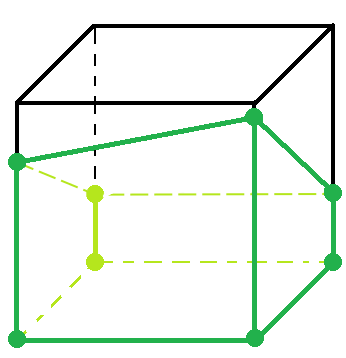
\includegraphics[ width=70mm]{../img/analysis/krychle}

\caption{Příklad nastavení polygonů}
\label{fig:polygons}

\end{figure}

\FloatBarrier

Obrázek \ref{fig:polygons} nám dává náhled nějakého možného uspořádání pěti polygonů v~rámci krychle. Silně vykreslené body představují definiční \textit{body}, jednotlivé čáry pak \textit{hrany} polygonů. Záměrně jsme neudělali polygony pravidelné, abychom demonstrovali, že je možné se libovolně přizpůsobovat tvarům vycházejícím z~polygonální reprezentace daného bloku.


V rámci algoritmu spojování bloků skrz vodivé spojení pak budeme hledat pro daný blok sousedy právě dle těchto definic. Budeme počítat s~tím, že polygony jsou v~rámci jedné roviny v~prostoru, přičemž daná rovina je rovnoběžná s~některou z~rovin mřížky herního světa. V~rámci této práce si algoritmus usnadníme takovým způsobem, že jednotlivé studované polygony rozšíříme na \textit{boxy}, tedy najdeme nejmenší možný kvádr, který je zarovnaný do mřížky definované herním světem (tedy nemá vůči ní žádnou rotaci) a~obsahuje všechny body z~daného polygonu\footnote{Abychom mohli použít standardních metod \TT{FBox::Intersect(...)}, musíme \textit{box} rozšířit o~něco netriviálního (např. $1~cm$) ve směru normály dané roviny.}. Za validní a~vodivé elektrické vedení pak budeme považovat takové dva polygony, které mají neprázdný průnik těchto boxů. Jsme si vědomi faktu, že tato úprava jde proti snahám hry o~vyšší stupeň realismu a~pro některé kombinace bloků dokonce bude porušovat naši definici vodivého spojení, ale v~této fázi nám to stačí a~nebudeme vyžadovat matematicky správné řešení.


\subsection{Objekt elektrické sítě}

Spojování bloků do elektrické sítě nevyžaduje žádnou speciální logiku. V~rámci přidávání bloku do herního světa budeme potřebovat vědět o~sousedních blocích (TODO stromy). Pokud bude vazba se sousedním blokem vyhodnocena jako validní vodivý spoj, může se nově připojený blok připojit ke stávající síti, v~níž je i~daný sousední blok.

Pokud budeme vycházet z~premisy, že každý blok je zapojen právě v~jedné elektrické síti a~všechny bloky v~rámci jedné elektrické sítě jsou mezi sebou vodivě spojeny, tak nutně musíme dojít k~závěru, že při manipulaci s~blokem budeme muset elektrické sítě aktualizovat. Přidáním bloku jsme bychom mohli vodivě propojit dvě či více sítí, při odebírání se nám daná elektrická síť může rozpadnout na více samostatných komponent. Těchto elektrických sítí může vznikat a~zanikat velké množství. Stačí si uvědomit, že k~bloku \nameref{blocks:A1} o~maximální možné velikosti můžeme připojit až 600 bloků, které budou patřit do stejné sítě (pro každou stěnu máme 100 bloků stejného typu a~minimální velikosti, uspořádaných do šachovnicového vzoru). Pokud pak odebereme centrální blok, může nám vzniknout právě až 600 nových elektrických sítí. Navíc, díky počasí se může stát, že bloky budou odebírány ze světa zcela neuspořádaně (na základě náhodně udělovaného poškození). Musíme tedy vymyslet algoritmus, jak pro všechny bloky v~herním světě udržovat správné informace o~jejich síti.

Protože nemůžeme nic předpokládat o~tom, jak se budou bloky v~elektrické síti chovat, musíme při změně (přidání či odebrání) nějakého bloku v~síti provést přepočítání. Nejjednodušší bude varianta na \textit{algoritmus vlny}. Jednotlivé sítě budeme podle potřeby odstraňovat či slévat. Popišme si nyní pravidla, která budeme muset ve hře mít. Jako sousedy budeme chápat bloky dostupné skrze vodivé spojení.

\subsubsection{Přidávání bloku}
Platí, že každý blok přidaný do herního světa si vytvoří svoji vlastní elektrickou síť.
(TODO kontrola enums níže)
\begin{enumerate}
	\item Pokud blok nemá žádné sousedy, nemusí dělat nic (svoji síť už má)
	\item Pokud mají všichni sousedé stejnou síť, blok se k~ní připojí
	\item Pokud mezi sousedy existují alespoň dvě různé elektrické sítě, blok si vytvoří novou elektrickou síť, propojí ji s~ostatními sítěmi a~vyvolá přepočet sítí
\end{enumerate}

\subsubsection{Odebírání bloku}
Platí, že každý odebíraný blok z~herního světa vždy odstraní síť, ve které je připojen, a~pro všechny jeho sousedy jsou vytvořeny nové sítě.

\begin{enumerate}
	\item Pokud blok nemá žádné sousedy, svoji síť ze hry odstraní a~dále nedělá nic
	\item Pokud má blok právě jednoho souseda, odpojí od se od dané sítě
	\item Pokud má alespoň dva sousedy, pro každého vytvoří novou síť a~vyvolá přepočet sítí
\end{enumerate}

\subsection{Udržování konzistence elektrických sítí}

Jak je vidět z~předchozí kapitoly, objektů k~aktualizaci může být velmi mnoho. Nesmíme však dopustit, aby se nám při přepočítávání začala hra zpomalovat či přímo zasekávat\footnote{Tato situace může snadno nastat, protože herní a~renderovací smyčky se na konci svých cyklů synchronizují, aby pro výpočet dalšího framu začínaly stejně.}. Opět máme více možností řešení, jak se k~tomuto problému postavit. 

Jedním z~možných řešení je spuštění výpočtů na samostatném výpočetním vlákně. Zde bohužel narážíme na problém, že výpočty ve vláknech v~\UEu{} nemohou přímo přistupovat k~herním objektům a~tudíž je nutné používat pomocných datových struktur a~výsledky poté zpětně propagovat. Kromě toho také narážíme na problém, kdy v~případě velmi silné bouře kyselých dešťů bude nejspíše často nutné výpočet předčasně ukončit a~spustit znovu.

My navrhujeme následující algoritmus, využívající front požadavků ke zpracování a~omezení výpočetního času. Ještě musíme zmínit, že také využívá toho, že jak elektrická síť, tak každý blok v~ní si nese informaci o~stavu. Ty jsou tři:
\begin{itemize}
	\item Nevalidní
	\item Ve výpočtu
	\item Validní
\end{itemize}
Volba stavů je zřejmá a~vychází z~principů algoritmu vlny. Dalším netriviálním faktem je, že v~algoritmu existuje fronta sítí k~přepočítání, přičemž každá taková má svoji frontu bloků v~síti k~přepočítání. Hlavním krokem algoritmu je pak výběr sítě k~přepočítání a~provedení jednoho kroku přepočtu. Následně, pokud má tato síť stále nějaké bloky k~přepočtu, je zařazena na konec přepočítávací fronty a~tam čeká, dokud nebude opět vyzvednuta. Může se však stát, že jistou posloupností kroků při mazání bude tato síť označena jako nevalidní a~dále se přepočítávat nebude.

Algoritmus bude mít přidělené nějaké maximální kvantum času, řekněme tak, aby při jeho výpočtech hra dosahovala alespoň 30 snímků za sekundu. Tím vcelku jednoduchým a~elegantním způsobem zajistíme přepočty i~pro velice rozsáhlé sítě. Samozřejmě je nutné, aby hra počítala s~tím, že elektrická síť a~bloky v~ní mohou být ve stavu \textit{ve výpočtu} a~tomu přizpůsobovat další funkcionalitu (například nevyužívat zdrojů takovéto sítě, dokud blok není \textit{validní} -- pak je možné využívat pouze dalších validních bloků, tedy těch, které již byly zpracovány algoritmem).

TODO tabulka případů, říct, že tohle bude komponenta

\subsection{Interakce a~označování}
\label{subsec:interaction}

Dalším problémem je interakce s~uživatelem. Abychom věděli, že hráč s~daným blokem chce interagovat, musíme vědět, že:
\begin{itemize}
	\item Je dostatečně blízko bloku
	\item Z~pohledu hráče se dívá na daný blok 
	\item Vyjadřuje fakt, že chce interagovat (např. stiskem klávesy)
\end{itemize}



Nejsnazší způsob, jak zjistit, na jaký herní objekt se hráč dívá, je použití techniky sledování paprsku (\textit{ray tracing}). Díky němu můžeme \uv{z kamery} vyslat virtuální paprsek, který má stejný směr, jako je směr pohledu kamery. Pokud bude hráčův \HUD{} zobrazovat zaměřovací kříž (či použijeme nějaký obdobný mechanismus) a~náš paprsek bude z~pohledu kamery tímto zaměřovačem procházet, hráč může cíleně mířit na herní objekty a~my zároveň budeme mít správnou informaci o~objektu, na který hráč zaměřovačem míří. Tento způsob získávání informace o~objektech v~hráčově zaměřovači je ve hrách běžný a~jeho použití je (pokud je vhodně použito) i~dostatečně rychlé.

Nyní, když už víme, jak můžeme získávat informace o~tom, na který objekt hráč míří, tak tento mechanismus ještě rozšíříme o~další vlastnost. Je zapotřebí si uvědomit, že interakce s~blokem a~umisťování nového herního bloku (případně mazání) jsou prakticky stejné akce. Liší se pouze výsledkem -- reakcí na stisk nějaké klávesy či tlačítka myši. Ale ve všech případech musíme vědět, na jaký blok hráč míří zaměřovačem, u~umisťování navíc potřebujeme znát i~přesný polygon, na který hráč míří. Konkrétní polygon potřebujeme znát z~toho důvodu, že chceme, aby se přidávaný blok \uv{přilepil} k~bloku, na který míříme. Tedy chceme zachovat herní mechaniku, která je v~hrách z~kapitoly \ref{chap:uvod} běžná a~je natolik intuitivní a~rozšířená, že změna této mechaniky by nejspíše nedopadla dobře a~hráči by nebyla kladně přijata.

Pro implementaci nám poslouží metoda \TT{LineTraceSingleByObjectType},\linebreak které předáme správné parametry (především počátek a~konec paprsku a~typy objektů, které paprsek zaznamená) a~ta nám vrátí strukturu, popisující výsledek trasování. Z~něj se můžeme dozvědět, jestli byl nějaký blok v~cestě paprsku. A~pokud ano, můžeme se ptát, zda měl komponentu interakce (potenciálně bychom mohli chtít bloky bez možnosti zaměření a~interakce, jakožto nesmazatelné objekty). Pokud bude i~tato podmínka splněna, můžeme se zajímat o~další vlastnosti kolize paprsku s~blokem a~na základě toho se nějak chovat.

Abychom hráči hraní usnadnili a~zpříjemnili, budeme bloky zvýrazňovat za použití techniky \textit{obrysu} (implementace zvýrazňování bude vycházet z~tutorialu~\citep{ue_outline_tut}). Tato technika je také využívána v~různých hrách napříč různými herními žánry a~proto její implementací nic nezkazíme. Obrys zobrazíme v~případě, kdy hráč nic nestaví a~daný označený blok je použitelný (takže hráč ví, že blok může používat), nebo v~případě, kdy hráč staví (zvýrazníme hranice namířeného objektu). Barvu obrysu můžeme zvolit kupříkladu zelenou pro použitelný blok, žlutou při stavění a~červenou při odebírání bloku. 


\subsection{Umístění ve světě}

Smyslem této komponenty je oddělení implementace bloku jako takového a~implementace herního světa. Skrze tuto komponentu se blok bude moci dotazovat na ostatní bloky v~herním světě, především pak bloky ve svém okolí. To bude důležité například pro elektrickou komponentu, která na základě \uv{sousedství} bude jednotlivé bloky vázat k~sobě do elektrické sítě.








\section{Definice bloků}
\label{sec:db}

Jak bylo řečeno v~analýze v~části \ref{sec:chceme}, potřebujeme u~bloků definovat mj.~následující vlastnosti: \textit{minimální} a~\textit{maximální} velikost, \textit{typ} bloku, možnost \textit{rotace} bloku dle daných os apod. Dále budeme u~bloků potřebovat zaznamenat, že blok má \textit{elektrickou} či \textit{kyslíkovou} komponentu a~definovat omezující vlastnosti této komponenty. Dále požadujeme, abychom mohli snadno modifikovat hodnoty těchto vlastností. Tento požadavek vznášíme z~toho důvodu, aby herní designér mohl rychle a~jednoduše ladit nastavení těchto konstant a~vyvažovat tak celkovou obtížnost hry. Takže nepřipadá v~úvahu, abychom měli tyto konstanty uložené ve zdrojovém kódu, protože jakákoliv úprava by znamenala opětovnou kompilaci hry a~to u~herních projektů často zabere netriviální čas. Pak je ale budeme muset načítat z~nějakého souboru, nebo budou muset být uložené v~nějakém definičním objektu, editovatelným z~Editoru.


\subsection{Textové soubory}
Při načítání definic z~textového souboru máme na výběr z~více možností. V~následujících odstavcích si jednotlivé možnosti popíšeme a~zamyslíme se nad výhodami a~nevýhodami daných přístupů. Jednu výhodu však mají všechny textové přístupy společnou -- snadnou čitelnost i~pro běžného člověka.

\subsubsection{Popis tabulkou}
Uvažme popis bloků v~nějakém tabulkovém formátu, třeba CSV. Pokud\linebreak bychom měli velice málo vlastností bloků, tento přístup by mohl být použitelný. Nicméně s~každým dalším nově přidaným blokem se do množiny všech vlastností mohou zanášet nové vlastnosti. To by znamenalo, že popis ostatních bloků, které danou vlastnost nemají, by musel nutně v~tomto tabulkovém zápisu uvažovat nějakou (byť prázdnou) hodnotu. Zbytečně by nám tak rostl definiční soubor. Další nevýhodou je absence typové bezpečnosti pro uložené hodnoty. 

\subsubsection{Popis samostatným souborem -- XML}
Běžné soubory textového formátu (TXT) není potřeba brát v~potaz. Výsledek je stejný jako při použití XML, ale nemůžeme zde použít definiční soubory pro automatickou kontrolu platnosti hodnot. Navíc bychom museli psát vlastní parser takového textového souboru, přičemž již hotové parsery XML jsou volně k~dispozici a~mohli bychom je snadno použít. Definici herních bloků v~XML využívá i~hra \ME{}. Tyto soubory jsou pak zpracovány herním enginem během načítání hry. Výhodou tohoto přístupu je, kromě snadného vytváření módu do hry, také snadná budoucí rozšiřovatelnost o~nové bloky.

\subsection{Binární zápis}
Binární zápis již není pro běžného člověka tak snadno čitelný, ale to nám nemusí vadit, pokud budeme mít k~dispozici příslušné editační rozhraní. My si totiž můžeme v~\UEu{} připravit třídu, jejíž vlastnosti jsou z~Editoru editovatelné pouze v~rámci nastavování výchozích hodnot. To znamená, že si na straně \CPP{} můžeme vhodným způsobem vytvořit strukturu definičních tříd, které následně použijeme v~Editoru. Na straně \UEu{} pak vytvoříme Blueprint, který bude dědit z~naší hlavní definiční třídy. Posléze můžeme této třídě upravovat výchozí hodnoty a~tímto způsobem tak definovat vlastnosti bloků.

Kromě toho, že tímto přístupem splňujeme požadavek na editovatelnost z~Editoru, získáváme také navíc typovou bezpečnost uložených hodnot. Dále máme možnost (v případě nějakých definičních specialit) vytvořit vlastní editační panely pro dané netriviální vlastnosti definičního souboru. 


\subsection{Definice bloků -- verdikt}

Na základě výše zmíněných poznatků jsme se rozhodli, že budeme bloky definovat v~binárním formátu. V~\CPP{} implementujeme definiční třídu s~vhodnou strukturou a~v~Editoru pak následně vytvoříme Blueprintové assety, ve kterých požadované vlastnosti pro námi požadované bloky nadefinujeme. Získáme tak možnost snadné úpravy požadovaných vlastností v~Editoru a~typovou bezpečnost vyplněných hodnot.

%!TEX root = ../../prace.tex


\section{Elektrická síť}
\label{sec:energyNet}
Účel elektrické sítě ve hře vychází z~reálného světa. Chceme, aby bloky spolu mezi sebou uměly komunikovat skrze nějakou síť a~aby přes tuto síť bylo možné automaticky převádět energii, třeba z~bloku \RB{B6} do bloku \RB{B8}. Na elektrickou síť nebudeme klást žádné omezující požadavky (například limitací přenosové kapacity bloků tvořících danou síť).

Pokud budeme vycházet z~premisy, že každý blok je zapojen právě v~jedné elektrické síti a~všechny bloky v~rámci jedné elektrické sítě jsou mezi sebou vodivě spojeny (viz kapitola \ref{subsec:encomp}), tak nutně musíme dojít k~závěru, že při manipulaci s~bloky budeme muset elektrické sítě aktualizovat. Přidáním bloku bychom mohli vodivě propojit dvě či více sítí, při odebírání se nám daná elektrická síť může rozpadnout na více samostatných komponent. Těchto elektrických sítí může vznikat a~zanikat velké množství. Stačí si uvědomit, že k~bloku \RB{A1} o~maximální možné velikosti můžeme připojit až 600 bloků, které budou patřit do stejné sítě (pro každou stěnu máme 100 bloků stejného typu a~minimální velikosti, uspořádaných do šachovnicového vzoru). Pokud pak odebereme centrální blok, může nám vzniknout právě až 600 nových elektrických sítí. Navíc, díky počasí se může stát, že bloky budou odebírány ze světa zcela neuspořádaně (na základě náhodně udělovaného poškození). Musíme tedy vymyslet algoritmus, jak pro všechny bloky v~herním světě udržovat správné informace o~jejich síti.

Protože nemůžeme nic předpokládat o~tom, jak se budou bloky v~elektrické síti chovat, musíme při změně (přidání či odebrání) nějakého bloku v~síti provést přepočítání a~to i~u~sítě, která již může být přepočítávána. Nejjednodušší bude varianta na \textit{algoritmus vlny}. Jednotlivé sítě budeme podle potřeby odstraňovat či slévat. 


Aby algoritmus vlny fungoval, je zapotřebí u~elektrické sítě a~každého bloku v~ní udržovat informaci o~stavu. Ty jsou tři:
\begin{itemize}
	\item Nevalidní
	\item Ve výpočtu
	\item Validní
\end{itemize}

Volba stavů je zřejmá a~vychází z~principů algoritmu vlny. Navíc tím můžeme požadovat, aby hra počítala s~tím, že elektrická síť a~bloky v~ní mohou být v~různých stavech a~tomu pak přizpůsobila svoji další funkcionalitu (například síť ve stavu \textit{ve výpočtu} nebude převádět zdroje sítě mezi bloky, které nejsou ve stavu \textit{validní} -- tedy těch, které již byly zpracovány algoritmem).

\subsection{Princip aktualizace sítě}

V předchozí části jsme zjistili, že nám může v~jednom okamžiku vzniknout velké množství sítí, jež je třeba aktualizovat. Navíc platí, že sítě mohou být rozsáhlé. Abychom co nejméně zasahovali do funkcionality aktualizovaných sítí, musíme nějakým způsobem zajistit, aby byla aktualizace sítí férová pro všechny sítě k~aktualizaci. Vzhledem k~tomu, že při nově vzniklém požadavku na aktualizaci sítě nevíme vůbec nic o~tom, které bloky nakonec v~dané síti budou, nemá smysl se zabývat myšlenkou upřednostňování aktualizace nějaké sítě vůči jiné, protože nemáme žádné faktické podklady pro to, jakou síť bychom měli upřednostnit.

Musíme tedy mít k~dispozici \textit{frontu sítí k~aktualizaci}. Každá síť z~této fronty si pak bude muset držet \textit{vlastní} frontu \textit{bloků k~aktualizaci}. V~algoritmu budeme postupně z~fronty vybírat sítě, provedeme u~nich krok algoritmu vlny a~případně je opět zařadíme do fronty. Tím zajistíme férovou aktualizaci pro všechny zúčastněné sítě.

Dále popíšeme, jak vypadá jeden krok algoritmu vlny. Jako sousedy budeme chápat bloky dostupné skrze vodivé spojení. Krok bude následující:

\begin{enumerate}
	\item Vyber blok \textbf{B} z~fronty bloků k~aktualizaci.
	\item Zkontroluj, že je \textbf{B} stále validní (zatímco \textbf{B} čekal ve frontě, mohl být mezitím zničen bouří kyselého deště). Pokud není validní, skonči.
	\item \textbf{B} označ jako \textit{Validní}.
	\item Pro všechny sousedy \textbf{S} bloku \textbf{B} se podívej na jejich síť a~stav bloku a~vykonej akci dle tabulky \ref{table:networkAlg}.
\end{enumerate}


\begin{table}[h]
\centering
\begin{tabular}{| l | l | l | l |}
	\hline
	Síť  \textbf{S}~~~$\backslash$~~ Stav \textbf{S}	& Nevalidní			& Ve výpočtu	& Validní 			\\ \hline
	Stejná jako \textbf{B}					& Naplánuj 	 		& Nic 			& Nic 	     			\\ \hline
	Jiná než \textbf{B} 						& \uv{Ukradni} a~naplánuj & Nic 			& Spoj sítě do jedné   	\\ \hline
\end{tabular}
\caption{Požadované bloky a~jejich základní vlastnosti}
\label{table:networkAlg}
\end{table}

\FloatBarrier

Abychom dobře pochopili význam akcí v~tabulce \ref{table:networkAlg}, měli bychom jednotlivé akce podrobněji popsat. Začněme situací, kdy je \textbf{S} ve stejné síti jako \textbf{B}.

Pokud je stav \textbf{S} \textit{Nevalidní}, pak musíme tento nalezený blok přidat do fronty bloků k~aktualizaci. Pokud je ve stavu \textit{Ve výpočtu}, pak je již naplánován, ale ještě nebyl zpracován (jinak by byl označen jako \textit{Validní}). Pokud je označen jako \textit{Validní}, byl již zpracován. Tyto kroky odpovídají standardnímu výpočtu algoritmu vlny. Pojďme se nyní podívat na situace, kdy jsou sítě \textbf{S} a~\textbf{B} \textit{odlišné}.

Pokud je stav \textbf{S} \textit{Nevalidní}, pak můžeme tento blok přiřadit do sítě \textbf{B} a~naplánovat ho ke zpracování. Určitě platí, že blok není v~žádné frontě ke zpracování (jinak by měl jiný stav). Pokud bychom ho \uv{neukradli}, zbytečně bychom tím ztratili cyklus kroku algoritmu. Navíc, jak je zmíněno v~části \ref{subsec:reac}, při odebírání je původní síť ponechána netknutá a~bloky jsou zneplatněny. Bez této vlastnosti bychom neuměli \uv{rozebrat} původní síť. Pokud je \textbf{S} ve stavu \textit{Ve výpočtu}, pak je již naplánován a~nemusíme dělat nic. Zde je důležitý fakt, že \textbf{S} bude někdy v~budoucnu vykonávat 4. krok algoritmu vlny a~tudíž nutně narazí na \textbf{B}, jakožto svého souseda s~jinou sítí. Ale protože \textbf{B} bude v~té době ve stavu \textit{Validní}, případ se tím převede na zbývající možnost. Když je \textbf{S} označen jako \textit{Validní}, pak musíme obě sítě spojit do jedné, protože všechny \textit{Validní} bloky z~obou sítí jsou propojeny skrze vodivé spojení \textbf{B} a~\textbf{S} a~tudíž musí mít i~stejnou síť.



\subsection{Reakce na přidání a~odebrání bloku}
\label{subsec:reac}
\subsubsection{Přidávání bloku}
Přidání bloku do systému elektrických sítí je jednoduché. Platí, že každý blok přidaný do herního světa si při přidávání vytvoří svoji vlastní elektrickou síť. Ta je pak přidána mezi všechny elektrické sítě v~herním světě a~je naplánovaná její \textit{aktualizace}. 

\subsubsection{Odebírání bloku}
Každý odebíraný blok z~herního světa vždy zneplatní celou síť, ke které je připojen (takže všechny bloky jsou v~nevalidním stavu), a~pro všechny jeho sousedy vytvoří nové sítě, které následně naplánuje k~\textit{aktualizaci}. Po dokončení všech aktualizačních výpočtů všech elektrických sítí je pak původní elektrická síť odstraněna. Dříve tak nesmíme učinit, protože bychom přišli o~vazby na bloky. Zde je také vidět, proč musíme umět \uv{krást} bloky.

\subsection{Optimalizace algoritmu}

Jak je vidět z~předchozí kapitoly, výpočtů v~aktualizaci může být velmi mnoho. Nesmíme však dopustit, aby se nám při přepočítávání začala hra zpomalovat či přímo zasekávat\footnote{Tato situace může snadno nastat, protože herní a~renderovací smyčky se na konci svých cyklů synchronizují, aby pro výpočet dalšího framu začínaly stejně.}. Opět máme více možností řešení, jak se k~tomuto problému postavit. 

Jedním z~možných řešení je spuštění výpočtů na samostatném výpočetním vlákně. Zde bohužel narážíme na problém, že výpočty ve vláknech v~\UEu{} nemohou přímo přistupovat k~herním objektům a~tudíž je nutné používat pomocných datových struktur a~výsledky poté zpětně propagovat. Kromě toho také narážíme na problém, kdy v~případě velmi silné bouře kyselých dešťů bude nejspíše často nutné výpočet předčasně ukončit a~spustit znovu.

Algoritmus bude mít přidělené nějaké maximální kvantum času, řekněme tolik, aby při jeho výpočtech hra dosahovala alespoň 30 snímků za sekundu. Pokud toto kvantum vyčerpá, nebude začínat další výpočty a~naplánovanou práci nechá do dalšího cyklu herní smyčky. Tím vcelku jednoduchým a~elegantním způsobem zajistíme aktualizace i~pro velice rozsáhlé sítě bez negativního vlivu na plynulost hry.








\section{Bloky v~herním světě}
\label{sec:blocksWorld}

Způsobů, jak reprezentovat bloky ve světě, je více, takže bychom měli jednotlivé varianty porovnat a~vyhodnotit. V~této chvíli si také musíme určit, jak velký chceme náš herní svět mít. Na základě tohoto důležitého požadavku budeme posuzovat vhodnost jednotlivých implementací. My jsme se rozhodli, že hráči nabídneme rozsáhlý svět čtvercového půdorysu o~rozloze $100\,\ km^2$ a~výšky $5\,\ km$. V~takto rozsáhlém herním světě bude mít hráč dostatek prostoru pro stavbu svých budov, a~to i~v~případě, že se v~budoucnu rozhodneme rozšiřovat hru o~nové bloky a~herní vlastnosti. Zároveň s~tím si ale uvědomujeme, že správně by hra měla řešit takto velký svět tak, aby i~velké množství bloků hru nezpomalovalo či dokonce neshodilo celou hru (třeba z~nedostatku paměti RAM). Nicméně jak jsme zmínili v~kapitole \ref{subsec:bloky}, budeme v~této práci očekávat takové množství bloků, jejichž počet hra bez problémů zvládne.

Námi definované hranice herního světa se u~bloků projeví tak, že v~rámci herního světa můžeme mít až $50~000 * 50~000 * 25~000$ bloků jednotkové velikosti, což je opravdu mnoho. Nejprve se tedy zaměříme na to, jak vůbec můžeme bloky reprezentovat a~zároveň s~tím budeme řešit, jak se vypořádat s~různými rozměry bloků.

\subsection{Použití dvourozměrného pole}

Představme si, že bychom herní svět reprezentovali polem. Pak bychom potřebovali 62~500~\textit{miliard} ukazatelů, z~nichž by naprostá většina byla prázdných (\textit{NULL}ových). Pro jednoduchost počítejme, že jeden ukazatel má velikost 4B a~že 1 kB je roven 1000 B. Pak dostáváme, že bychom potřebovali alokovat 250~TB dat. To vidíme jako problém, takže se zkusme zaměřit na efektivnější datové struktury.

\subsection{Stromové struktury}
\label{subsec:trees}

Jako rozumný nápad se jeví použití stromových struktur, které nám budou reprezentovat svět podle skutečně zabraných pozic v~herním světě. Kdybychom povolili volnou počáteční rotaci, zřejmě bychom museli přistoupit k~nějaké variantě \textit{clusterů}, tedy shluků bloků ve stejné ortogonální mřížce. Protože tuto vlastnost nepovolujeme, můžeme se zabývat jinými datovými strukturami. Ve hrách jsou běžně používané například:


\begin{itemize}
	\item Octree
	\item K-D stromy
\end{itemize}

Pojďme si tedy tyto možnosti rozebrat a~zhodnotit v~kontextu naší hry.

\subsubsection{Octree}
Octree je stromová datová struktura, ve které vrchol reprezentuje nějaký objem a~jeho 8 potomků tento objem rovnoměrně dělí na menší části. Obvykle vrcholy této struktury reprezentují krychle v~nějakém prostoru. Pokud se zamyslíme, jak by náš svět byl v~této struktuře reprezentován, dojdeme k~tomu, že kořenový vrchol této struktury by měl 4 potomky vždy prázdné. Ačkoliv to není nijak zásadní nevýhoda, podívejme se na alternativní řešení.

\subsubsection{K-D strom}
K-D strom je datová struktura, která je velmi podobná Octree, ale na rozdíl od ní má pouze 2 potomky. Vrchol, který se nachází v~nějaké hladině, totiž svůj objem rozdělí do dvou polovin v~závislosti na dané hladině. Takto je možné reprezentovat vícedimenziální prostory, kdy jednotlivé hladiny reprezentují dělení pro jednotlivé souřadnice. Každá následující hladina této struktury pak představuje dělení podle následující souřadnice v~daném prostoru. Pro n-dimenzionální prostor pak (n+1) hladina (počítáno od jedné) opět dělí prostor podle první souřadnice.

\subsubsection{Vlastní rozšíření K-D stromu}
K-D strom je pro naši situaci vhodnější, protože při správné implementaci této struktury můžeme změnit rozměry herního světa (pokud to bude potřeba) a~nebudeme muset měnit implementaci reprezentace bloků v~herním světě. V~rámci našeho rozšíření navrhujeme, aby si jednotlivé vrcholy uchovávaly informaci o~reprezentované části herního světa v~podobě Min-Max boxu\footnote{Jako Min-Max box budeme chápat strukturu, která je popsána dvěma vektory, které představují minimální a~maximální hranice. Ve 2D prostředí by to byl obdélník s~udáním levého dolního rohu a~pravého horního rohu.}. Tuto vlastnost pak využijeme pro rychlé dotazování nad tímto stromem (například při kontrole, zda je možné nějaký blok umístit na nějakou pozici v~herním světě). Navíc budeme chtít, aby byla hloubka stromu co nejmenší, takže navrhujeme optimalizaci, kdy blok ve stromě může být v~daném vrcholu uložen jako \uv{jedináček}. Tento blok může být umístěn kdekoliv v~prostoru, který daný vrchol reprezentuje. 

\subsection{Reprezentace bloku}

Abychom si usnadnili indexování bloků, budeme uvažovat, že bloky jsou\linebreak v~osách X a~Y indexovány v~intervalu <-25~000, 25~000>. V~ose Z~(tedy vertikální ose) budeme bloky indexovat v~intervalu <0, 25~000> a~indexy ve všech osách budou celočíselné. Dále určíme fakt, že jednotkový blok na herních souřadnicích [0, 0, 0] bude v~\UEu{} reprezentován na pozici [0, 0, 0]. 

\subsubsection{Střed bloku a~škálování}
Pro potřeby porozumění následujícího textu se přesuneme z~3D prostoru, ve kterém v~\UEu{} pracujeme, do 1D prostoru. Jednotkovou úsečkou budeme rozumět úsečku o~délce $20\,\ cm$ (chceme zde zachovat konzistenci s~požadavkem na minimální velikost bloku z~kapitoly \ref{subsec:bloky}). Tuto jednotkovou úsečku umístíme na osu tak, že střed úsečky je přesně ve středu osy. Tudíž kraje jednotkové úsečky jsou v~bodech [-10], [10].

Nyní potřebujeme určit body osy, ke kterým budeme střed jednotkové úsečky přichytávat. To budou přesně $k$-násobky délky jednotkové úsečky pro libovolné celočíselné $k$. Nyní můžeme říci, že pokud budeme chtít umístit jednotkovou úsečku na $n$-tý index osy, střed této jednotkové úsečky bude v~bodě $(n * 20)$ a~kraje jednotkové úsečky budou v~bodech $[(n * 20) -- 10]$ a~$[(n * 20) + 10]$. Vidíme, že kraje jednotkové úsečky jsou správně zarovnané a~pro $n = 0$ odpovídají umístění jednotkové úsečky.

Nyní si představme situaci, kdy chceme na osu umístit jednotkovou úsečku zvětšenou na \textit{dvojnásobek} (označme ji \textbf{D}). Zvětšování je symetrické dle středu a~po umístění \textbf{D} na \textit{nultý} index osy dostáváme, že kraje \textbf{D} jsou v~bodech [-20], [20]. Nyní vidíme, že kraje \textbf{D} nejsou správně zarovnané, protože prochází námi definovanými body pro přichytávání. Kdybychom teď chtěli na index 1 umístit jednotkovou úsečku, obě úsečky se nám protínají a~to je špatně -- chceme dosáhnout toho, aby i~při libovolném zvětšení jednotkové úsečky byla tato úsečka správně zarovnaná.

Je důležité si uvědomit, že problém z~předchozího odstavce vzniká (díky symetrii zvětšování) pouze při škálování \textit{sudým} číslem. Pro tato čísla musíme udělat to, že si střed bloku \uv{virtuálně} posuneme tak, abychom celou škálovanou úsečku správně zarovnali do námi definovaných hranic (tento virtuální střed budeme správně přichytávat k~ose). Při určování virtuálního středu se budeme řídit pravidlem \uv{nejbližšího nižšího} možného středu. 

Demonstrujme posouvání virtuálního středu následujícím příkladem.\linebreak Vezměme si čtyřnásobně zvětšenou jednotkovou úsečku, označme si ji jako \textbf{Č}. Budeme ji chtít umístit na \textit{nultý} index osy. Bez posouvání středu bychom řekli, že hranice úsečky jsou v~bodech [-40], [40]. Představme si \textbf{Č} rozloženou na jednotkové úsečky, zleva indexované od 0. Nyní máme střed na indexu [$1,5$], tedy \textit{mezi} jednotkovými úsečkami 1 a~2. Pravidlem \uv{nejbližšího nižšího} virtuálně posuneme střed \textbf{Č} na index [1]. Když pak jednotkou úsečku na indexu [1] správně přichytíme k~ose, hranice se nám posunou o~$10\,\ cm$ doprava, kraje \textbf{Č} budou v~bodech [-30], [50] a~tím dosáhneme správného zarovnání.

Posledním krokem je rozšíření výše uvedených myšlenek na všechny tři souřadnice 3D prostoru. Nyní už víme, jaký způsobem budeme řešit zarovnání bloku o~nějaké škále na daných \textit{herních} souřadnicích. Zároveň z~toho můžeme vidět, jakým způsobem budeme postupovat při převodu z~našeho souřadnicového systému do systému souřadnic v~rámci \UEu{}.
 
\subsubsection{Důsledky škálování}

Z výše uvedených faktů je vidět, že ve hře budou muset existovat pravidla pro výpočty mezi souřadnicovým systémem naší hry a~souřadnicovým systémem \UEu{}. Dále z~toho vyplývá, že pokud má blok netriviální škálování, dle výše uvedených pravidel může inherentně \uv{zabrat} některé pozice v~našem souřadnicovém systému a~jiné bloky pak tento prostor nemohou obývat. To je skvělý výsledek, protože tím máme vyřešené konkrétní pozice a~nemohou nám nastat konflikty umístění bloků.

Dalším důležitým důsledkem je způsob rotací škálovaných bloků. Budeme chtít, aby blok rotoval vzhledem k~\textit{virtuálnímu} středu. 

Dále máme usnadněné výpočty hranic bloku vůči globálnímu souřadnicovému systému \UEu{}. K~tomu nám stačí znát umístění v~našem souřadnicovém systému, velikosti a~rotaci bloku. Výsledkem pak může být Min-Max box, který můžeme použít pro dotazy nad naším K-D stromem. Jednoduchým a~rychlým výpočtem pak můžeme analyzovat, jestli mají nějaké dva bloky nějaký netriviální průnik, jestli se dotýkají apod.


\subsubsection{Důsledky reprezentace bloků na herní svět}

Budeme chtít, aby jednotlivé vrcholy našeho K-D stromu znaly svoji reprezentaci v~podobě Min-Max boxu. Tím získáme výhodu rychlého vyhodnocení dotazů (kupříkladu zda je možné umístit nový blok na nějaké souřadnice udané hráčem). Dále, budeme chtít, aby bloky měly vazbu na náš K-D strom. Cílem je dosáhnout toho, aby blok mohl vyhledávat své sousedy \uv{odspodu} a~jejich hledání tak bylo velmi rychlé.


\subsection{Zapojení do rozpoznávání tvarů}
\label{subsec:adrt}

Vzhledem k~dynamicky škálovatelným blokům budeme požadovat, aby bylo možné bloky skládat do tvarů libovolným splňujícím způsobem. Tedy by mělo být jedno, zda do tvaru umístíme jeden blok velikosti [1, 1, 2], nebo dva jednotkové bloky vedle sebe. Představu o~tomto konceptu si lze udělat z~obrázku \ref{fig:konfig}, který zobrazuje 4 splňující varianty stejného tvaru.

\begin{figure}[!ht]\centering
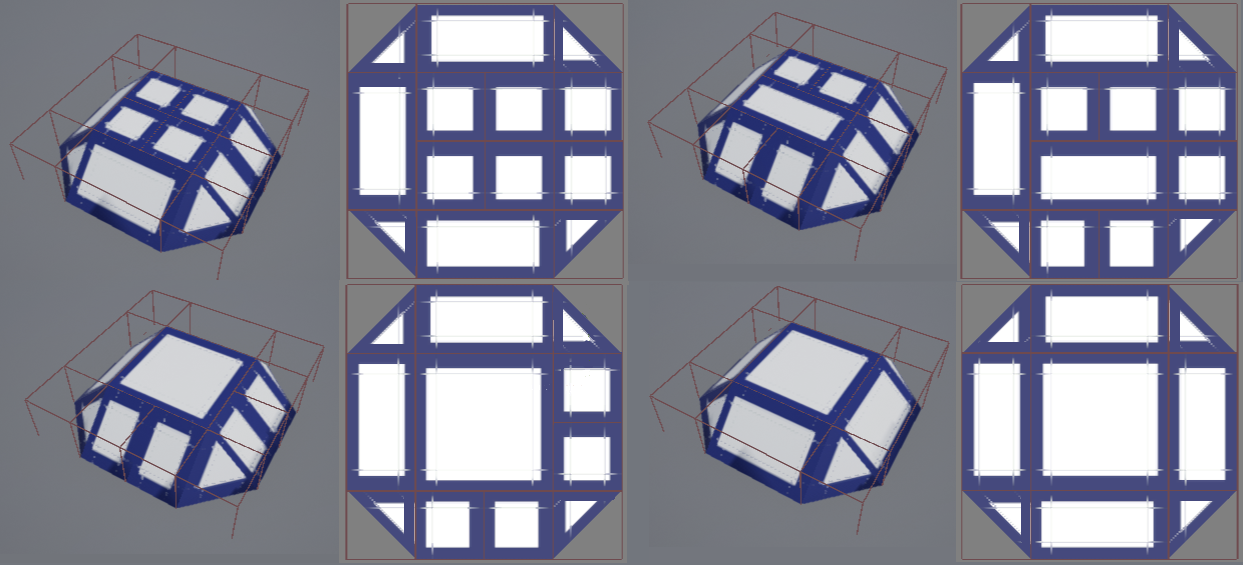
\includegraphics[ width=140mm]{../img/analysis/konfigurace}

\caption{Ekvivalentní konfigurace tvaru. Zdroj: StackOverflow.com~\citep{so_pattern}}
\label{fig:konfig}

\end{figure}

\FloatBarrier

\subsubsection{Komplexní systém rozpoznávání tvarů}
Výše zmíněný přístup k~rozpoznávání tvarů však přináší mnoho nových problémů. Pro příklad uvažme rozklad bloku \RB{A5} netriviální velikosti (kupříkladu [2,~1,~2], tedy šířky jednotkového bloku). Je zřejmé, že stejného tvaru je možné dosáhnout použitím dvou stejných bloků velikosti [1,~1,~1] a~jednoho bloku \RB{A2} velikosti [1,~1,~1] (pokud budeme uvažovat, že je možné tyto dva bloky vzájemně kombinovat). Bloky v~herním světě by se pak musely nějakým způsobem sdružovat do těchto vyšších celků a~ty pak vyhodnocovat vůči definovaným tvarům, či případně jinak rozpoznávat, zda jsou součástí nějakého předem definovaného tvaru. Z~důvodu celkové náročnosti tohoto přístupu jsme se rozhodli, že tento komplexní systém nebudeme v~naší práci požadovat. Nicméně, tato myšlenka se nám velice líbí, takže ji necháme jako možné budoucí rozšíření této práce.






%!TEX root = ../prace.tex

\section{Počasí}

- počasí chceme proměnlivé ale s tím, že gamedesignéři mohou snadno ovlňovat výsledné počasí, případně aby šlo snadno rozšířit varianty pro různé herní módy

-budeme mít ve světě umístenou entitu (Pawn) ovládaný AI Controllerem - to z toho důvodu, že pro AI Controller můžeme použít BehaviorTree

-popsat ideu BT

-další možnosti by byly, že bychom prostě použili update smyčku nějakého Actora - není potřeba, tohle se vyřeší updatem na komponentě

%!TEX root = ../prace.tex

\section{Hráčova postava}

- pohled 1st person, 3rd person

- má komponenty kyslíku, energie

- může stavět, interagovat s bloky

- může zařvat


%!TEX root = ../../prace.tex

\section{Inventář}

Inventář bude vhodné implementovat jako komponentu, kterou posléze můžeme přiřadit herní postavě. Opět se zde opíráme o~fakt, že bychom v~budoucnu mohli mít bloky či \NPC{}, kteří také mají svůj inventář. Z~kapitoly \ref{subsec:inventory} vyplývá, že inventář má několik základních vlastností:

\begin{itemize}
	\item Seznam postavitelných bloků
	\item Seznam umístitelných bloků
	\item Seznam inventárních skupin pro filtrování
\end{itemize}

V momentě, kdy budeme chtít hráči nabídnout bloky k~postavení či umístění, oba seznamy dofiltrujeme dle aktuálně zvolené inventární skupiny. Musíme se tedy zaměřit na to, jak budeme řešit inventární skupiny.

\subsection{Inventární skupiny}

Protože má každý blok své definované \textit{tagy}, musíme vymyslet takový systém, abychom snadno filtrovali podle těchto tagů. Nejsnazší způsob je takový, kdy každá inventární skupina definuje, jaké tagy musí blok mít, aby byl přiřazen. Takže pro blok, který má být zobrazen v~rámci inventární skupiny, platí, že blok definuje všechny tagy v~rámci dané inventární skupiny. Nicméně se může stát, že hráč bude chtít mít v~dané skupině takové bloky, které nemusí splňovat všechny tagy, ale splňují alespoň jeden z~definované skupiny. Z~této myšlenky se dostáváme k~jednoznačnému způsobu filtrování tagů, který je ekvivalentní s~\textit{konjunktivně normální formou} (\CNF{}).


Chceme tedy implementovat takový systém, kdy \textit{inventární skupina} definuje \textit{inventární skupiny tagů} (konjunktivní vyhodnocení), přičemž \textit{inventární skupiny tagů} definují \textit{skupiny tagů} (disjunktivní vyhodnocení). Při vyhodnocování \textit{inventární skupiny} budeme sledovat, zda blok splňuje všechny její \textit{inventární skupiny tagů}, přičemž pro každou z~nich budeme zjišťovat, zda blok definuje alespoň jeden tag ze \textit{skupiny tagů}. 

Abychom hráči ještě více zpříjemnili práci s~inventářem, nebudeme požadovat přesnou shodu tagů definovaných blokem a~\textit{skupinou tagů}. Bude nám totiž stačit pouze podmínka podřetězce, tedy podmínka, aby tag bloku obsahoval jako podřetězec tag ze \textit{skupiny tagů}. Tím dosáhneme toho, že hráč nebude muset v~inventáři vypisovat celé řetězce z~tagů, které si nadefinoval u~svých bloků. 





%!TEX root = ../../prace.tex

\section{Ukládání hry}

- vše se musí korektně uložit

- ?? specifikace binárního formátu zde, nebo v programátorský?

%!TEX root = ../prace.tex

\section{Doplňující vlastnosti}

\subsection{DLC}

- můžeme dodávat extra bloky (ukázka!)

\subsection{Lokalizace}

- použití lokalizace 

\subsection{Hudba}

- atmosférický hudební doprovod




\section{Backlog}

\begin{itemize}
	
	\item Popsat, že bychom chtěli nějaké UI + nabídky menu

\end{itemize}

%!TEX root = ../prace.tex

\chapter{Programátorská dokumentace}

%!TEX root = ../../prace.tex

\section{Počáteční inicializace projektu}

Pokud je cílem spustit projekt hry ze zdrojových kódů, je potřeba si stáhnout \UE{} ve verzi \TT{4.15.3}. Na hlavní stránce \UE{} je potřeba stáhnout \textit{Epic Games Launcher} (ke stažení zde~\citep{ue_download}). Po vytvoření uživatelského účtu a~následnému přihlášení do aplikace bude vidět obrazovka podobná obrázku \ref{fig:ueLauncher}:


\begin{figure}[!ht]\centering
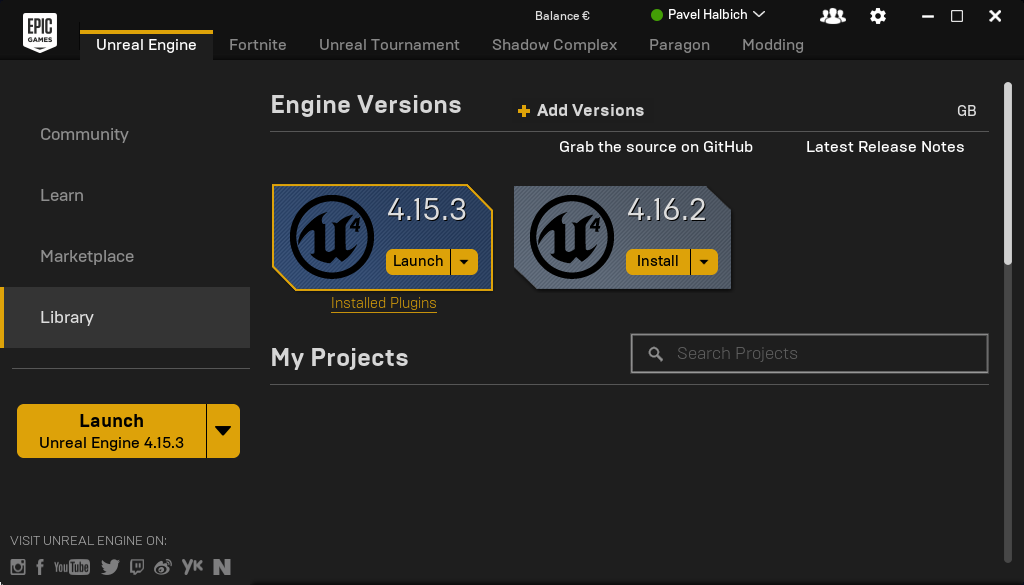
\includegraphics[ width=140mm]{../img/program/ueLauncher}

\caption{Epic Games Launcher}
\label{fig:ueLauncher}

\end{figure}

\FloatBarrier

Pokud není vidět \UE{} dané verze v~seznamu verzí, je potřeba jej přidat kliknutím na tlačítko \textit{Add Versions} a~případném následném výběru správné verze. Na obrázku \ref{fig:ueLauncher} je vidět \UE{} verze \TT{4.16.2}, který je připravený ke stažení. Posledním krokem je samotná instalace stisknutím tlačítka \textit{Install}. Použití novější verze \UEu{} je možné, ale běžnému uživateli to nedoporučujeme. Mezi verzemi se mohou projevit nekompatibility v~kódu, které je mnohdy nutné řešit zásahy přímo do zdrojových kódů hry.

TODO lépe popsat, že se vytváří VS projekt ze zdrojáků -- je to standardníá

Dále je potřeba mít k~dispozici zdrojové kódy ať už z~DVD, nebo z~tohoto release na GitHubu (TODO link na public repo, release commit).
 
Následujícím krokem je vytvoření projektu hry. Toho se docílí kliknutím pravým tlačítkem myši na soubor \TT{TauCetiF2.uproject} a~následnou volbou \textit{Generate Visual Studio project files} (viz obrázek \ref{fig:generateProjectFiles}). 

\begin{figure}[!ht]\centering
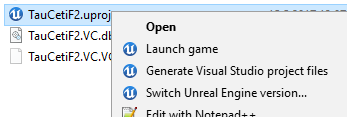
\includegraphics[ width=80mm]{../img/program/generateProjectFiles}

\caption{Vytvoření projektu hry}
\label{fig:generateProjectFiles}

\end{figure}

\FloatBarrier


Pokud v~kontextové nabídce chybí možnosti pro \UE{}, je potřeba provést asociaci s~\TT{uproject} soubory. Tato asociace by měla být provedena automaticky, nejpozději po vytvoření libovolného \CPP{} projektu z~kterékoliv šablony Ze zkušenosti autora -- toto se mnohdy nemusí podařit. Pokud se nepodaří vygenerovat projekt hry, může pomoci otevřít editor přes \textit{Epic Games Launcher}, najít a~otevřít projekt a~po načtení vybrat možnost obnovy projektu, jak je naznačeno na obrázku \ref{fig:ue_refresh}. K~tomu je zapotřebí mít Visual Studio 2015 alespoň ve verzi \textit{Community}.


\begin{figure}[!ht]\centering
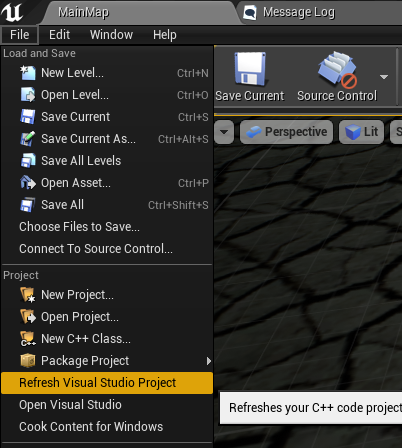
\includegraphics[ width=80mm]{../img/program/ue_refresh}

\caption{Vygenerovaný projekt hry}
\label{fig:ue_refresh}

\end{figure}

\FloatBarrier



Pokud i~toto selže, ověřte si, prosím, že je možné založit nějaký projekt založený na \CPP{}, zkompilovat jej a~taktéž vygenerovat projekt pro Visual Studio. Pokud se to povede s~projektem z~nějaké připravené šablony, mělo by to fungovat i~s~naší hrou.


Předposledním krokem je v~případě úspěšného vytvoření projektu hry jeho otevření ve \textit{Visual Studiu}, nastavení \textit{TauCetiF2} jako hlavní spustitelnou část projektu (viz obrázek \ref{fig:vs}) a~následné spuštění  editoru hry.


\begin{figure}[!ht]\centering
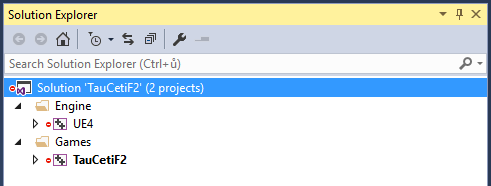
\includegraphics[ width=110mm]{../img/program/vs}

\caption{Vygenerování projektu hry}
\label{fig:vs}

\end{figure}

\FloatBarrier





%!TEX root = ../../prace.tex

\section{Struktura projektu}

Strukturu přhodit do analýzy

Celý projekt je rozdělen do dvou částí -- \CPP{} část a~Blueprintová část. \UE{} umožňuje herním vývojářům implementovat celou hru kompletně za pomocí Blueprintů, tedy vizuálního rozhraní. Toho se však obvykle nevyužívá, protože vykonávání programu v~Blueprintu je přibližně 10 krát pomalejší, než vykonávání nativního \CPP{} kódu (TODO link). V praxi tak dochází k~tomu, že vývojář (i neprogramátor) může za pomocí Blueprintů rychle prototypovat funkcionalitu, kterou pak kodér přepíše do metod v~\CPP{}, správně tyto metody označí makry tak, aby \UE{} tyto metody v~kódu našel (což se provádí za pomocí reflexe v~\UBT{} a~použitím příslušných \CPP{} maker) a~upraví Blueprint tak, aby původní kód tyto metody volal.

 V Blueprintu je kód vizualizován jako graf uzlů a~jsou zde zaznamenány vztahy mezi těmito uzly. Uzly tedy odpovídají funkcím v~\CPP{} a~těm je pak možné předávat parametry ať už v~podobě proměnných definovaných v~\CPP{} kódu nějaké třídy, nebo proměnných definovaných přímo v~Blueprintu. Vztahy mezi uzly pak označují následující kód určený k~vykonávání. Můžeme také říct, že vykonávání kódu v~Blueprintu je \textit{interpretované}, z~čehož vyplývá absence případných kompilačních optimalizací. Ergo slabý výkon. 

Některé části programu jsou implementovány na úrovni \CPP{}, jiné bylo nutné implementovat v~Blueprintech. Už víme, že komunikace z~Blueprintu do \CPP{} je možná prostým voláním metod, ale určitě budeme potřebovat i~možnost opačného směru. Toho je možné dosáhnout více způsoby -- kupříkladu použitím delegátů a~událostí (Blueprint se pak na tuto událost naváže a~v~případě vyvolání dané události vyvolá v~Blueprintu definovanou obsluhu), nebo BlueprintImplementable či BlueprintNative metod. (TODO formátování!, link na Specifikaci?) Poslední dvě nám nabízí možnost, jak volat virtuální metody, které je možné přepisovat jak na straně \CPP{}, tak na straně Blueprintu, což se nám bude hodit.

V dalším textu tedy postupně probereme prvně kódovou část napsanou v~\CPP{} a~poté strukturu projektu s~samotném \UE{}. Ještě bychom zde měli zmínit, že ačkoliv se v~textu budeme odkazovat převážně na hlavičkové soubory, stále budeme brát v~potaz i~implementační, tedy \TT{.cpp} soubory a~obsah textu se může na tuto implementaci odkazovat.



%!TEX root = ../../prace.tex

\section{Struktura kódu}
\label{sec:struct}

Protože jsme zvolili implementaci práce v~\UE{}, můžeme využít toho, že engine umožňuje rozdělit celý herní projekt do jednotlivých herních modulů~\citep{epicGameplayModules}. Tím docílíme modularity, nebudeme mít celý projekt v~jednom kuse a~zároveň tím urychlíme překlad projektu při kompilaci.\\
Každý \UE{} projekt musí definovat právě jeden primární herní modul. Pokud využijeme možnosti vytvoření nového projektu založeného na \CPP{}, editor tento modul automaticky vytvoří za nás. My jsme pojmenovali náš projekt {\tt TauCetiF2} a~tak se jmenuje i~náš primární modul.

Jednotlivé části projektu jsme rozdělili do několika herních modulů:

\begin{enumerate}
	\item TauCetiF2 (primární modul)
	\item Inventory
	\item Blocks
	\item Game Save
	\item Commons
\end{enumerate}

Herní moduly jsme seřadili dle jejich závislosti tak, že každý modul závisí na všech modulech s~vyšším očíslováním. Tedy primární modul využívá všech ostatních modulů a~poslední modul (Commons) není závislý na žádném dalším modulu. Pro lepší představu můžeme tyto souvislosti vyjádřit obrázkem \ref{fig:obrStruktura_DependencyDiag}: 

\begin{figure}[!ht]\centering
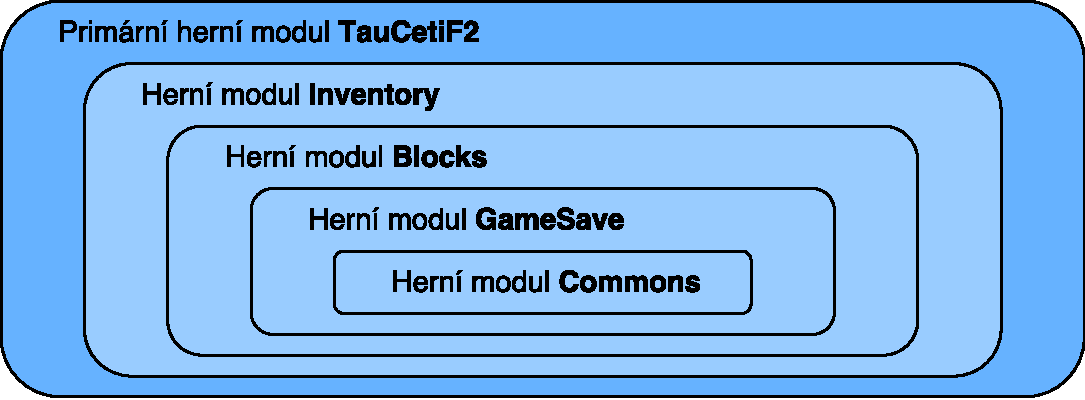
\includegraphics[ width=140mm]{../img/dependencyDiagram}

\caption{Diagram závislostí modulů projektu.}
\label{fig:obrStruktura_DependencyDiag}

\end{figure}

\FloatBarrier

Obecnou koncepci programu jsme popsali v~kapitole \ref{sec:ueStructure}. Abychom se vyhnuli velkému množství dopředných referencí, strukturu programu z~pohledu \CPP{} budeme popisovat od nejnižších vrstev.

\subsection{Obecná struktura modulu}
Všechny moduly dodržují společnou strukturu. Obsahují:
\begin{itemize}
	\item složku \verb!Public!
	\item složku \verb!Private!
	\item soubor \verb![název_modulu].Build.cs!
	\item soubory \verb![název_modulu].h!, \verb![název_modulu].cpp!
\end{itemize}


Každý modul pak má hlavičkové soubory ve složce \TT{Public}, implementaci tříd pak ve složce \TT{Private}. Soubor \TT{*.Build.cs} je využíván nástrojem \UBT{}, zbylé dva soubory definují herní modul v~rámci \UEu{}.




%!TEX root = ../prace.tex

\section{Modul Commons (C++)}

Tento modul je základním modulem, který na jednom místě definuje všechny potřebné informace, které využívají ostatní moduly. Jedná se zejména o definici herních konstant, či definice všech sdílených enumerátorů. Najdeme zde také prapředka použité herní instance. Tuto vlastní implementaci herní instanci využijeme pro ukládání nalezených bloků.

\subsection{Herní definice a konstanty}

\TT{GameDefinitions.h}

Tady jsou definovány všechny herní konstanty. Například je zde definována velikost jednotkové krychle, velikost použitého světa, vztah mezi délkou dne herního světa a počtem uplynulých reálných sekund, převody mezi energií, kyslíkem, zdraví a jednotkou zásahu kyselého deště. Taktéž jsou zde definovány konstanty, které využívá technika obrysů objektu (todo link na outline). Dále jsou zde definovány konstanty ID implementovaných bloků, abychom s nimi mohli pracovat i v kódu.

\subsection{Herní instance}
\TT{TCF2GameInstance.h}

Tato třída je Singleton ( TODO link UE docs) a jako jediná zůstává vždy stejná po celou dobu běhu hry. Proto se využívá například pro uchovávání dat při přechodu mezi jednotlivými Levely a my toho také využijeme. Zároveň se tato třída dá využít pro implementaci delegátů, kterými je možné vyvolat nějakou událost a libovolný prvek z herního světa může tuto událost obsloužit. My toho využijeme u reakce na denní cyklus u bloku \textit{Přepínače}.

Dalším důležitým bodem pro nás bude, že tato třída si bude držet referenci na všechny nalezené bloky. Z předchozího textu již víme, že bloky je potenciálně možné rozšířit o DLC (TODO budem to tu řešit?), takže je nutné, abychom si nalezené bloky a jejich definice udrželi v paměti i při přechodu mezi levely. K tomu slouží proměnná \TT{BlockHolder} , která sice  drží referenci na objekt definovaný v modulu \textit{Blocks}, ale kvůli zpětným referencím mezi moduly (které nejsou povolené) musíme zde použít dostupného předka.

Kód tedy bude vypadat následovně:
\begin{code}
	UPROPERTY(Transient)
		UObject* BlockHolder;

	UFUNCTION(BlueprintCallable, Category = "TCF2 | GameInstance")
		void SetHolderInstance(UObject* holder);
\end{code}
 Parametr \TT{Transient} u makra \TT{UPROPERTY} znamená, že daná proměnná bude vždy nastavena na svoji výchozí hodnotu. V tomto případě je to použito spíše z důvodu zachování konzistence napříč projektu, ale zjednodušeně bychom důsledky mohli popsat následovně -- pokud bude nějaký Blueprint dědit z nějaké \CPP{} třídy, tak vývojář může nastavit výchozí hodnoty properties. Tyto hodnoty jsou pak serializovány do CDO (TODO link?). Během procesu vytváření nové instance objektu, který vychází z daného Blueprintu pak budou tyto hodnoty naplněny během fáze inicializace properties (TODO link na Actor life time?). V konečném důsledku by pak byla tato hodnota nějakým způsobem naplněna. Pokud chceme vynutit, aby tato property nebyla serializována do CDO, tak ji označíme jako \TT{Transient}.

Holder pro nalezené bloky (TODO popsat proč)

\subsection{Enumerátory}

\TT{Enums.h}

co tam je (vypsat všechny, nebo jenom řáct, že je to definované zde, protože je to pro celý projekt?)

\subsection{FFileVisitor}

Kvůli nalezení savů
TODO link na systém ukládání.

\subsection{Helpery}

helpery pro načítání / ukládání konfigurace (vlastních polí)

popsat že UE má mechanismus automatického ukládání vlastností do konfiguračníh souborů, ale to nám nevyhovovalo
%!TEX root = ../../prace.tex

\section{Modul Game Save (C++)}

Modul GameSave slouží k~ukládání a~načítání informací o~probíhající hře do binárního formátu. K~tomu používáme streamové operátory $<<$, které jsou v~tomto případě implementovány tak, že je možné je použít jak pro ukládání, tak pro načítání. // TODO link na tutorial

Díky tomuto přístupu tak můžeme definovat celou strukturu výsledného binárního souboru na jednom místě a~tedy rozšiřování uložené hry je triviální. Co si ovšem musíme pohlídat je to, abychom si drželi informaci o~verzi uloženého souboru. V~našem případě, pokud se bude lišit verze načteného souboru a~uložená konstanta v~programu, save prostě odmítneme (a dokonce smažeme). V~produkčním prostředí bychom si mazání nemohli dovolit, ale museli bychom save ignorovat a~uživateli zobrazit nějakou hlášku o~tom, že verze souboru není podporovaná. My jsme se však v~tomto případě rozhodli save mazat, protože jsme očekávali, že během vývoje hry se bude binární struktura savu často rozšiřovat. Po každé iteraci jsme si savy prostě vytvořili nové.

Zamysleme se nad tím, co by se stalo, kdybychom se snažili načíst save jiné verze. Celá hra by nejspíše byla ukončena s~chybou, protože by se pokoušela číst neplatná data a/nebo by očekávala nějaká data tam, kde žádná nejsou. Tím bychom četli z~neplatné lokace.




\subsection{GameSaveInterface}

\TT{UGameSaveInterface.h} 
Tento soubor definuje rozhraní, které je možné implementovat a~používat v~Blueprintech (struktura vychází z~tutoriálu na Unreal Engine Wiki~\citep{ue_interfaces_tut}). Rozhraní definuje dvě veřejné metody, které musí actoři v~UE při implementaci tohoto rozhraní implementovat:

\begin{code}
UFUNCTION(BlueprintNativeEvent, BlueprintCallable, ... )
	bool SaveGame();

UFUNCTION(BlueprintNativeEvent, BlueprintCallable, ... )
	bool LoadGame();
\end{code}

Hlavní Blueprint levelu pak během svého běhu určité actory přetypuje na tento interface a~bude s~nimi dále pracovat. Podrobněji tato funkcionalita bude popsána v~Blueprintové části.

\subsection{FFileVisitor}

\TT{FFileVisitor.h}

Tento soubor obsahuje implementaci návrhového vzoru Visitor pro získání všech herních savů z~nějaké zadané složky. Implementace vychází z~internetové diskuse na téma procházení adresářů~\citep{ue_iterate_dir}.

\subsection{Helpers}

\TT{SaveHelpers.h}
Tento soubor řeší získání seznamu všech uložených her a~využívá k~tomu implementaci FileVisitoru z~předchozí části.

\subsection{Kontejner s~uloženou hrou}
\TT{SaveGameCarrier.h} Tato třída je v~zásadě přepravkou pro data s~možností ukládání a~načítání dat do binárního formátu. Navíc umožňuje během ukládání v~době vývoje vypsat vlastnosti právě ukládané hry do konzole tak, abychom mohli během vývoje snadno tento výstup zkopírovat a~vytvořit pevně implementované hry. Tyto pevně implementované hry pak nebudou data vracet po přečtení nějakého binárního souboru, ale budou vracet pevně nastavená data. Vytváření těchto pevně vytvořených her pak bylo o~dost jednodušší.

Přepravka obsahuje pouze holá data, tedy nevytvářejí se žádné nové instance herních objektů. To je z~toho důvodu, že nemůžeme použít následující kód:

\begin{code}

// vlastnost kontejneru
TArray<UBlockInfo> UsedBlocks;

// během ukládání
void USaveGameCarrier::SaveLoadData(
	FArchive& Ar,
	USaveGameCarrier& carrier,
	TArray<FText>& errorList,
	bool bFullObject)
{
	Ar << carrier.UsedBlocks;
}
\end{code}
Museli bychom mít referenci na datový typ \TT{UBlockInfo}, který je ale definovaný v~modulu Blocks, který musí nutně modul GameSave referencovat. Tudíž zde použijeme následující konstrukci:

\begin{code}
// vlastnost kontejneru
TArray<FBlockInfo> usedBlocks;

// během ukládání
void USaveGameCarrier::SaveLoadData(
	FArchive& Ar,
	USaveGameCarrier& carrier,
	TArray<FText>& errorList,
	bool bFullObject)
{
	Ar << carrier.usedBlocks;
}
\end{code}

Třídu dědící z~UObjektu jsme nahradili strukturou \TT{FBlockInfo}, která sama slouží pouze jako přepravka na data. Vyšší vrstva, tedy modul Blocks si těmito daty naplní své vlastní objekty, které se pak dále využívají ve hře. A~naopak, před samotným uložením se postará o~to, aby bylo toto pole korektně naplněno všemi daty určenými k~uložení. O~samotnou serializaci a~deserializaci dat do a~z~přepravky se stará pouze modul GameSave.

Celý systém vychází z~tutoriálu~\citep{ue_save_system} je postaven na tom, že v~C++ je možné přetěžovat operátory, mimo jiné i~$<<$. Této vlastnosti je využito tak šikovně, že v~závislosti na volání funkce buď zapisuje do archivu, nebo z~něj čte, ale pořád se jedná o~jediný zápis jedné funkce. To je výhodné, protože to předchází chybám, které by mohly vzniknout při použití 2 metod -- jedné čtecí, jedné zapisovací. Chybám typu přehození dvou datových typů (což by v~případě typů různých velikostí znamenalo následné špatné pochopení binárních dat), nebo kupříkladu prohození dvou vlastností stejného typu, což by vytvářelo těžko odhalitelné situace změn hodnot ve hře.

Tento systém je použit pro všechny rozšířené části herního savu -- Bloky, Inventář, Počasí -- a~všechny používají podobný způsob práce. Jedná se o~definici struktur, tedy samotných kontejnerů a~dále pak jeden soubor pojmenovaný \TT{*ArchiveHelpers.h}, kde je popsána vlastní struktura daných kontejnerů v~Archivu. Hvězdičku v~tomto případě bereme opravdu jako zástupný symbol. Navíc, některé objekty mohou řídit archivaci dle nějakých podmínek nastavených shora. Příkladem budiž definice serializace elektrické komponenty:

\begin{code}
// přetížení, které se nevolá vždy
FORCEINLINE FArchive& operator<<(
	FArchive &Ar,
	FPoweredBlockInfo& componentInfo)
{
	Ar << componentInfo.IsOn;
	Ar << componentInfo.AutoregulatePower;
	Ar << componentInfo.PowerConsumptionPercent;
	return Ar;
}

FORCEINLINE FArchive& operator<<(
	FArchive &Ar, 
	FElectricityComponentInfo& componentInfo)
{
	Ar << componentInfo.CurrentObjectEnergy;
	Ar << componentInfo.HasPoweredBlockInfo;

	// pokud máme navíc rozšiřující data, přidáme další data
	// tím efektivně zavoláme metodu uvedenou výše
	if (componentInfo.HasPoweredBlockInfo)
		Ar << componentInfo.PoweredBlockInfo;

	return Ar;
}
\end{code}

Jak vidíme z~kódu, celý kód se chová korektně jak při serializaci, tak i~při deserializaci. Je pouze potřeba vzít v~úvahu, že vyšší struktury, které pak budou tyto data používat pro vlastní inicializaci, musí také brát v~potaz podmínku. Pokud není splněna, tak svázaná proměnná (v tomto případě \TT{PoweredBlockInfo}) nebude obsahovat platná data.

\subsection{NewGameSaveHolder}

\TT{NewGameSaveHolder.h} Tato třída je hlavní třídou, se kterou hra před načítáním pracuje. Definuje seznam napevno zabudovaných levelů a~obsahuje jejich implementaci.










%!TEX root = ../prace.tex

\section{Modul Blocks (C++)}

Modul bloků obsahuje podstatné informace o tom, jak hra pracuje s bloky, jak se tyto bloky skládají do herního světa, jaké jsou jejich komponenty apod. Také je v tomto modulu možné nalézt specifické implementace jednotlivých bloků.

V dalším textu se budeme odkazovat na složky. Odkazujeme se tím do složek \TT{/Source/Blocks/Public} a jejich  \TT{Private} implementací. Strukturu bychom mohli shrnout následovně:

\begin{enumerate}
	\item Definice bloků (složka \TT{Definitions})
	\item Třídy s popisem bloků (složka \TT{Info})
	\item Systém ukládání a načítání bloků (složka  \TT{Helpers})
	\item Rozhraní, které mohou bloky implementovat (složka \TT{Interfaces})
	\item Komponenty, kterými bloky rozšiřují svoji základní funkcionalitu (složka \TT{Components})
	\item Implementace jednotlivých bloků (složky \TT{BaseShapes}, \TT{Special})
	\item Stromové struktury herního světa (složka \TT{Tree})
\end{enumerate}
 

\subsection{Definice bloků}
V této složce se nachází všechny definiční soubory bloků. Definiční soubor obsahuje pouze popis datové struktury a nějakou minimální funkcionalitu (kupříkladu získání korektního vektoru velikosti v závislosti na tom, zda má definice daného bloku nastavenou vlastní velikost). Jednotlivé konkrétní instance s daty jsou pak definovány na straně editoru. Konstanty (například minimální a maximální škálování) je pak možné měnit v editoru a není vyžadována rekompilace projektu hry. 

Definiční soubor se skládá následujícím způsobem:

\begin{itemize}
	\item UBlockDefinition (\TT{BlockDefinition.h})
		\subitem -- FUsableBlockDefinition (\TT{UsableBlockDefinition.h})
		\subitem -- FBlockMeshStructureDefinition (\TT{BlockMeshStructureDefinition.h})
			\subsubitem -- FBlockMaterialDefinition (\TT{BlockMaterialDefinition.h})
		\subitem -- FBlockAdditionalFlags (\TT{BlockAdditionalFlags.h})
			\subsubitem -- FBlockFlagValue (\TT{BlockFlagValue.h})	
		\subitem -- FOxygenComponentDefinition (\TT{OxygenComponentDefinition.h})
		\subitem -- FElectricityComponentDefinition (\TT{ElectricityComponentDefinition.h})
			\subsubitem -- FElectricityBindableAreas (\TT{ElectricityBindableAreas.h})	
				
		

\end{itemize}

\subsection{Třídy s popisem bloků}
Tyto třídy popisují už konkrétní instance bloků v rámci hry. Jejich hodnoty jsou pak v mezích definovaných v definičních třídách. Tyto třídy jsou pak předmětem ukládání a načítání. Dalším důležitým prvkem je BlockHolder, který slouží pro nalezení bloků. 

\subsection{Ukládání a načítání bloků}

- ukládání - máme něco jako block saving helpers


\subsection{Interfaces}
poskytují nástroje pro volání metod na instaních interfacu

popsat ideu za Implementation, Execute (BlueprintNativeEvent, BlueprintImplementableEvent)

\subsection{Komponenty bloků}
- pak máme komponenty bloků a nějaké interfaces

\subsubsection{Elektrická komponenta}


\subsubsection{Elektrická síť}


\subsubsection{Kyslíková komponenta}


\subsubsection{Select target}


\subsubsection{World object}






\subsection{Implementace bloků}
 - základ Block.h, zbytek v jendotlivých podkategoriích (BaseShapes / Special
 
 TODO jak moc podrobné? vypsat všechny bloky a co všechno implementují, nebo to stačí stručně zmínit? - co implementují by si čtenář mohl uvědomit z předchozího textu a navíc je to jen nudný popis, jehož výžpovědní hodnota je ve zdrojácích a není asi nutné to tu duplikovat

- popsat speciální bloky + nějaké speciality co umějí (showableWidget)


\subsection{Stromové struktury}
popsat stromové struktury, které tam mám


\subsubsection{MinMaxBox}

prapředek všeho



\subsubsection{KDTree}

dědí z MMB, základ ve světě


\subsubsection{WeatherTargetsKDTree}

dědí z MMB, slouží pro potřeby počasí
%!TEX root = ../prace.tex



\section{Modul Inventory (C++)}

Modul inventáře byl vyčleněn do samostatné části. Je to hlavně jako ukázka možného členění do modulů. Navíc časem by se mohl tento modul rozšířovat jak by rostla kompelxicita správy inventáře.

Nejdůležitější inventory component


\subsection{Tag group}
nejnižší úroveň, odpovídá 'nebo'

\subsection{Inventory tag group}

celá skupina, odpovídá 'A zároveň'

\subsection{Inventory tags}

sdružuje všechny banky

\subsection{Inventory component}

celá komponenta, která je pak navázaná na hráčův charakter

definuje delegáty notifikující o změnách v akivní skupině, po filtrování apod.

na této úrovni se řeší aktualizace cache buildable i inventorybuildable při změnách, zároveň poskytuje možnost clear cache pro volání shora (BP)


%!TEX root = ../prace.tex

\section{Modul TauCetiF2 (C++)}
- primární modul

popsat co všechno obsahuje (widgety, gamemodes, weather apod)

- popsat synchronize widget ( // TODO link na důvod, proč to tam mám), popsat object widget, napsat důvody

- popsat to stackování 

- popsat komponenty
(weather, game electricity)






%!TEX root = ../../prace.tex

\section{Struktura projektu v~Unreal Enginu}
\label{sec:ueStructure}

- ukázat jak se to dělí v~UE editoru

Struktura složek

\begin{itemize}
	\item Složka XY
\end{itemize}

Popsat lokalizaci

\subsection{Mapy}

Základní částí projektu v~\UE{u} je \textit{herní mapa}. Ta obsahuje všechny důležité herní objekty.

popsat jednotlivé mapy, jaký je jejich cíl

a



\section{Backlog}

Zde popsat jak jsem to celé implementoval a~proč


Popsat jednotlivé C++ třídy a~jejich odvozené Blueprintové deriváty + přidat případné obrázky z~BL kódu (např. BlueprintImplementable event, který se zavolá jak na C++ tak i~na BP) 

Udělat rozbor BT počasí + mechaniku počasí + denního cyklu
popsat řízení osvětlení dle počasí

Udělat rozbor bloků, škálování, konfigurace, datovou strukturu, implementaci dynamických textur, zvýraznění

Popsat mechaniku Selector -- SelectTarget + napojení na Builder

Popsat mechaniku používání objektů + zvýraznění

-> Mám svět, ten má v~sobě bloky, ty jsou v~nějaké stromové struktuře, bloky mají komponenty, které přes tuto strukturu mohou na sebe vázat
Svět má také počasí se svojí vlastní strukturou, vuyžívající podobnosti s~bloky (2D KD strom s~Heapem na listech)

-> hráč může to a~tamto, díky inventáři se dostane na bloky, a~díky selectoru je pak můževložit do světa skrz World controller (zmíněno v~předchozím)
->zároveň jsou všechny entity savovatelné 


-> Popsat struktury Widgetů, zmínit použití Synchronize Widgetu, implementaci mechaniky stackovatelných widgetů

-> popsat implementaci hudby




// TODO obrázky s~konfiguračními ukázkami do příloh (např. jak se definuje Blok z~UE



%!TEX root = ../prace.tex

\chapter{Uživatelská dokumentace}

\section{Požadavky pro spuštění hry}
\subsubsection{Hardwarové požadavky}

Doporučená minimální sestava (na ní byla hra vyvíjena): 

\begin{center}
	\begin{tabular} { | l | l |}
		\hline
		Procesor: 	&	Intel i7-2630QM @ 2.00GHz \\	\hline
		RAM:		&	12 GB	(8 GB by mělo také stačit) \\	\hline
		Grafika:	&	ATI Radeon HD 6700M \\	\hline
		OS:			&	Win 10 x64	(7 a~vyšší by měly též fungovat) \\
		\hline
	\end{tabular}
\end{center}

Výše uvedneou konfiguraci je potřeba brát jako orientační. Hru jsme úspěšně spustili i~na notebooku s~procesorem Intel i5, integrovanou grafickou kartou a~8 GB operační paměti. Bylo však nutné nastavit grafické vlastnosti na minimální možnou konfiguraci. 

\subsubsection{Softwarové požadavky}

Pro spuštění zkompilované hry není potřeba nic speciálního. Je zapotřebí mít stroj s~minimální uvedenou konfigurací. Dále je dobré mít nainstalované poslední verze ovladačů HW komponent (hlavně grafiky). Taktéž je zapotřebí mít nainstalovanou poslední verzi DirectX a~C++ runtime. Tyto části lze doinstalovat z~přiloženého DVD ze složky \textit{Redist}.


\section{Tutoriál}
Tato hra obsahuje pokročilý tutoriál, ve kterém se lze snadno naučit veškeré principy hry. Ten je dostupný z~dialogu výběru nové hry. Proto se nebudeme zabývat podrobným popisem uživatelské dokumentace.
\begin{figure}[!ht]\centering
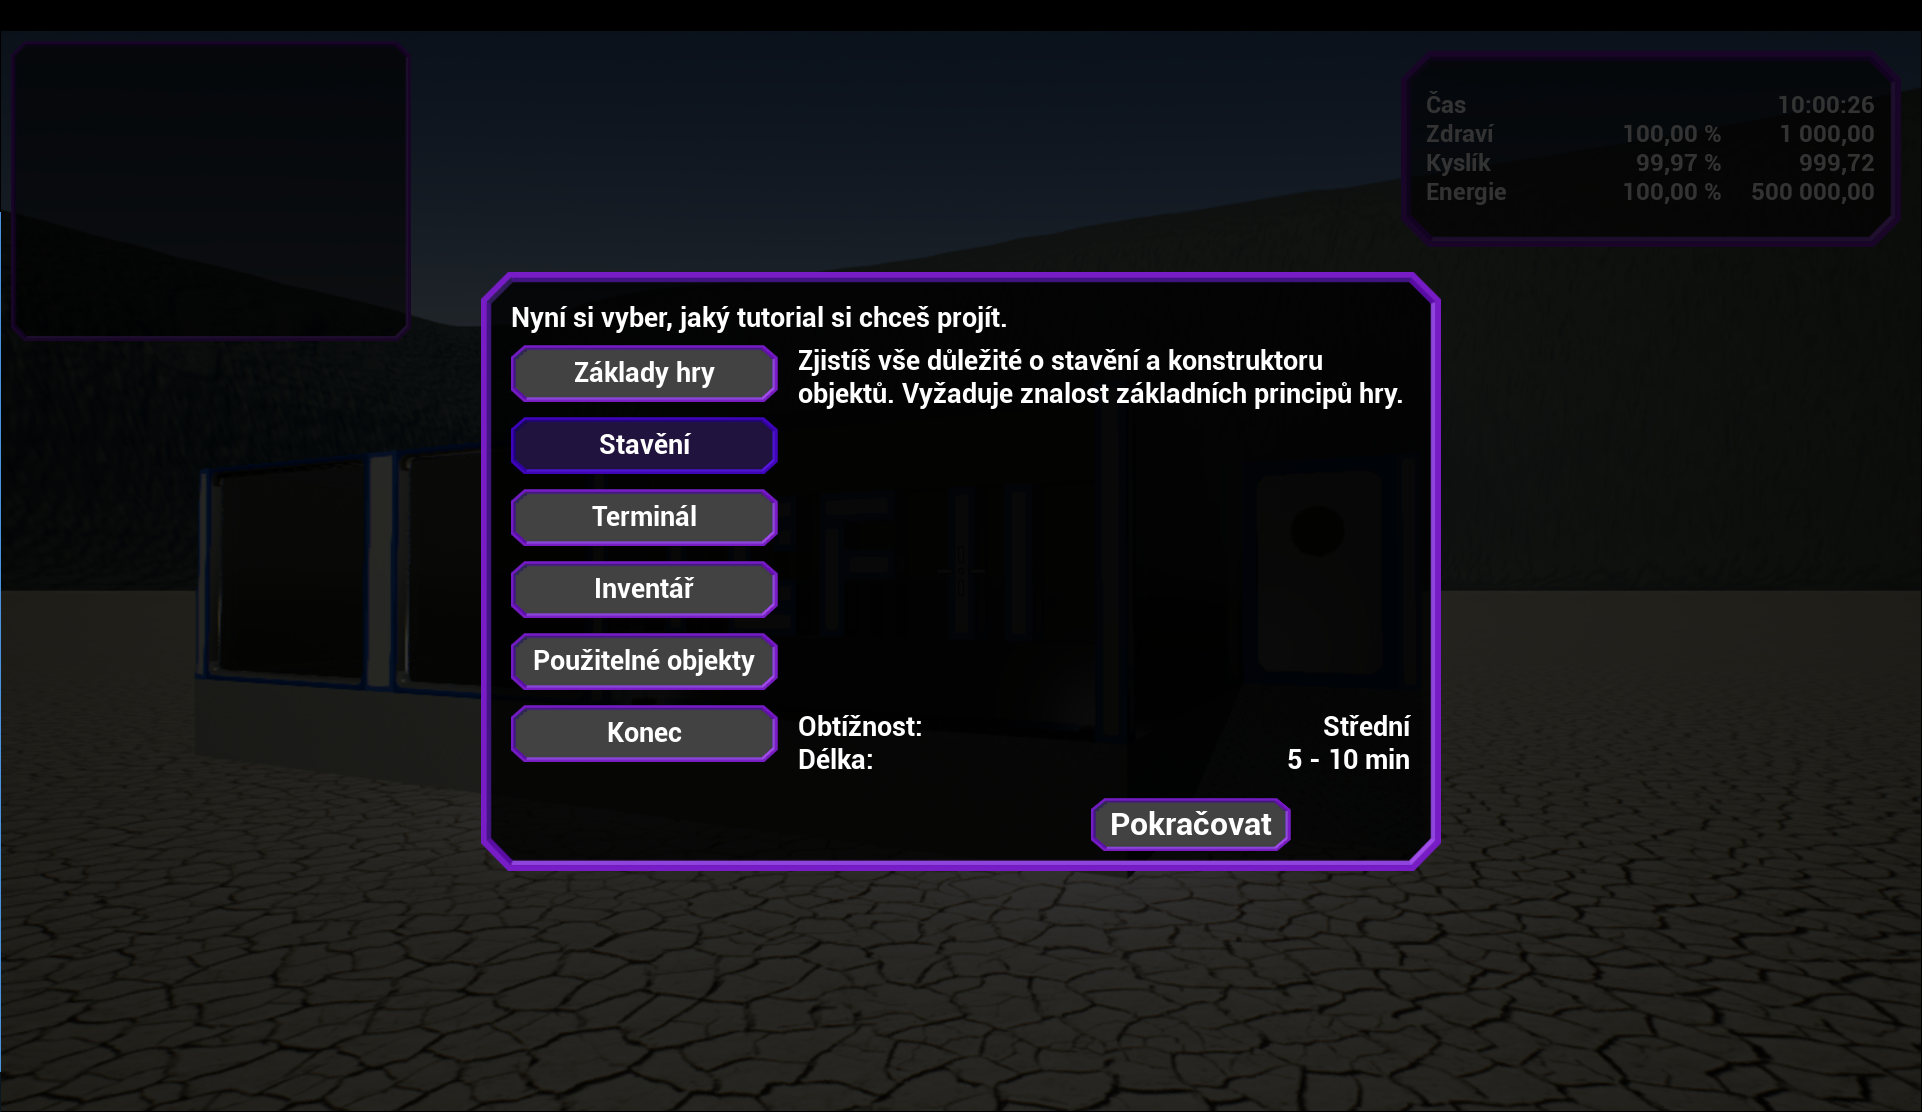
\includegraphics[ width=140mm]{../img/user/mainMenu/mmTut}

\caption{Výběr herního tutoriálu}
\label{fig:usr_tut}

\end{figure}
\FloatBarrier


%!TEX root = ../../prace.tex

\section{Hlavní menu}

Po načtení hry hráč vidí hlavní menu. Denní doba i~počasí se zvolí náhodně.

\begin{figure}[!ht]\centering
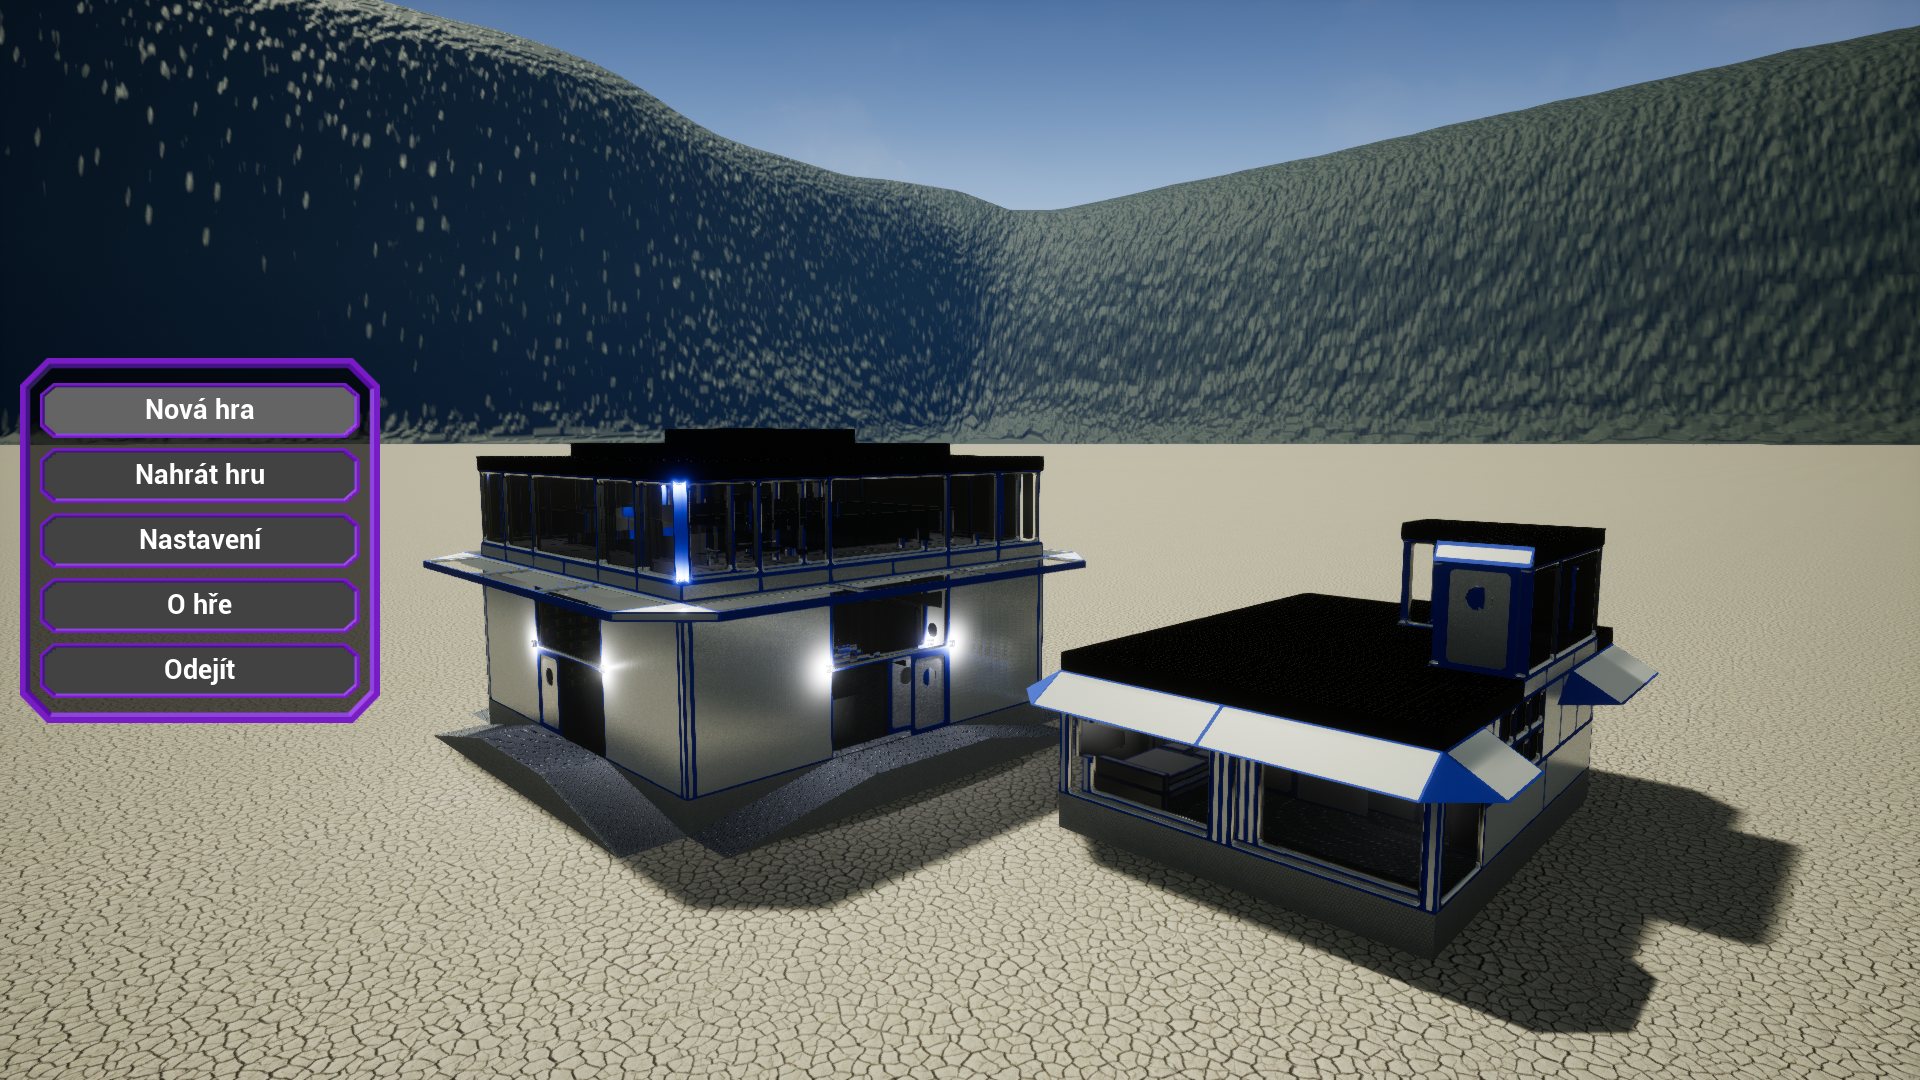
\includegraphics[ width=140mm]{../img/user/mainMenu/mmDay}

\caption{Obrazovka hlavního menu -- den}
\label{fig:user_mainMenu_mmDay}

\end{figure}


\FloatBarrier

První volba, kterou je možné zvolit, je výběr nové hry. K~dispozici je několik variant s~různými obtížnostmi.

\begin{figure}[!ht]\centering
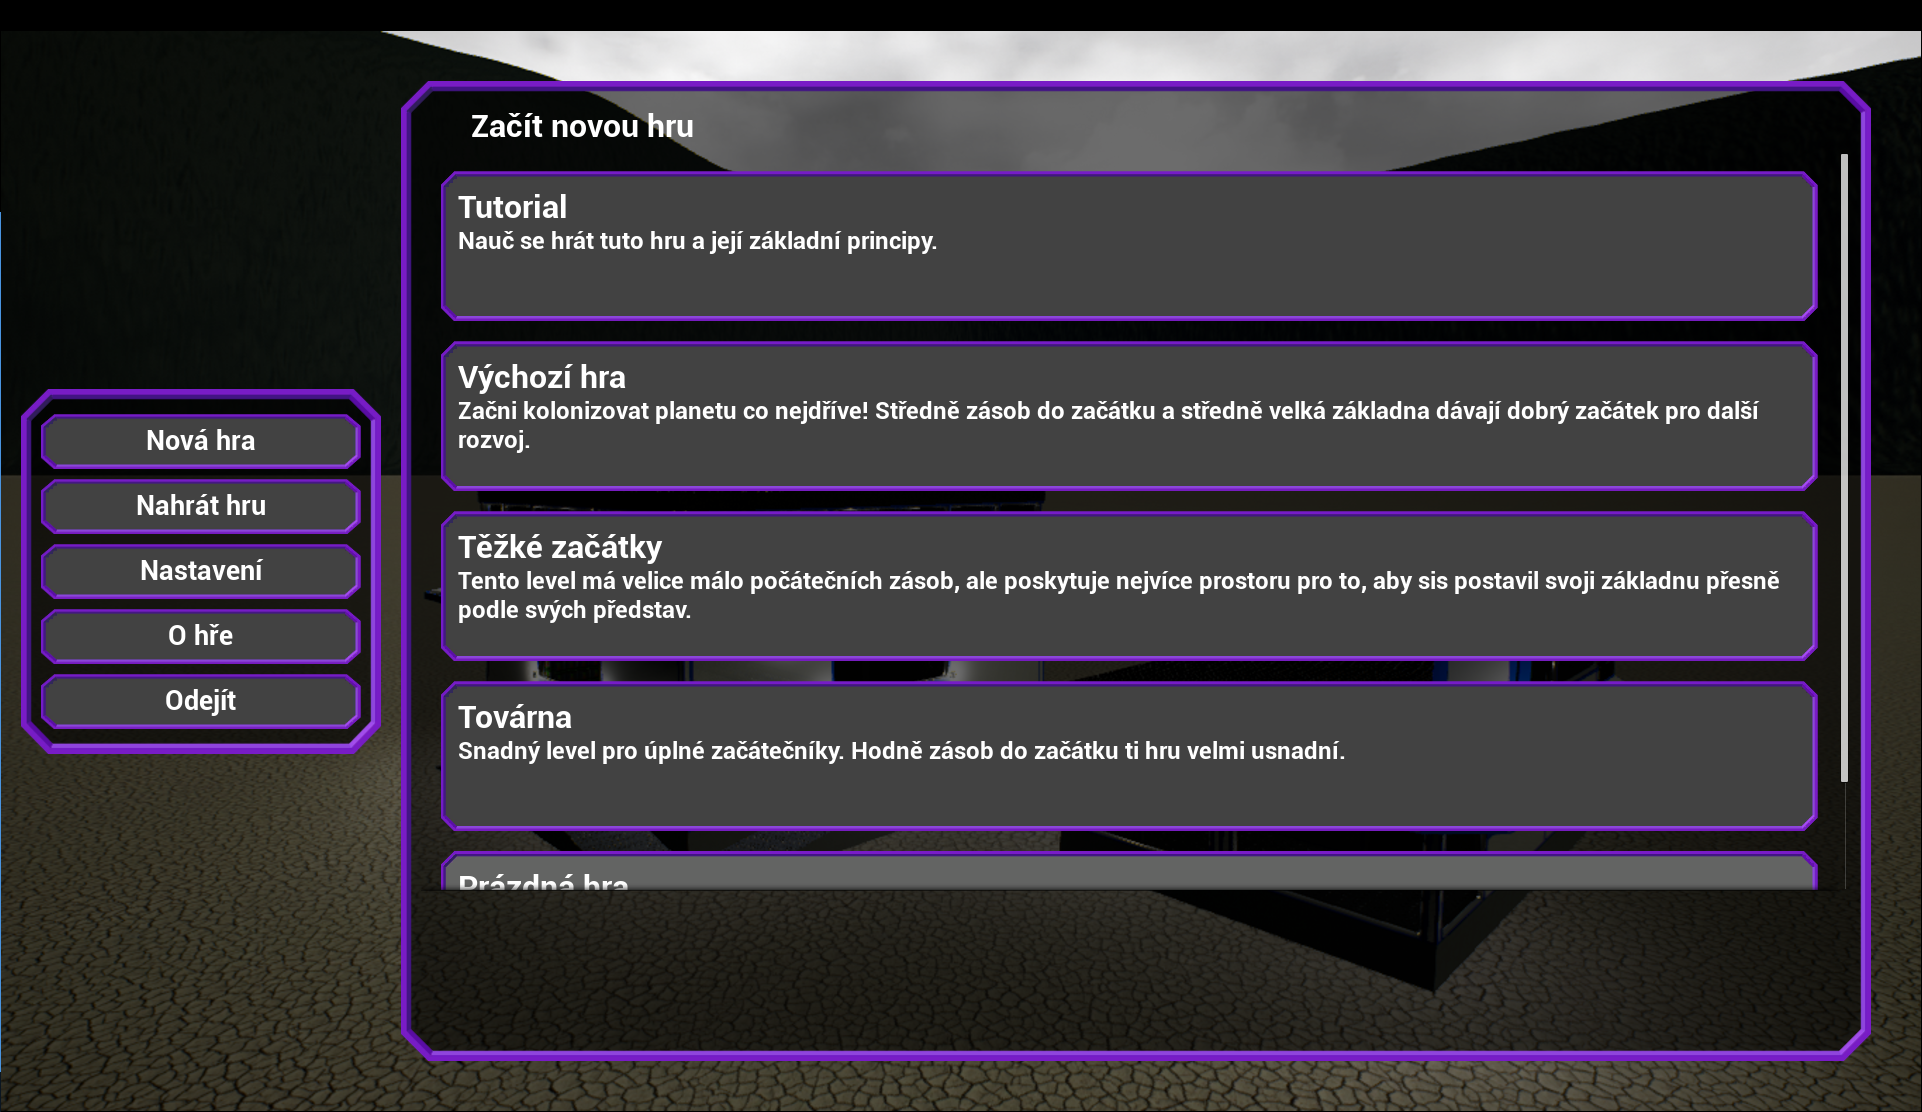
\includegraphics[ width=140mm]{../img/user/mainMenu/mmBegin}

\caption{Obrazovka hlavního menu -- Nová hra}
\label{fig:user_mainMenu_mmBegin}

\end{figure}
\FloatBarrier

Pokud hráč má nějaké uložené hry, může si je nahrát kliknutím na tlačítko \textbf{Nahrát hru}. V~tomto případě žádné uložené hry k~načtení k~dispozici nejsou.

\begin{figure}[!ht]\centering
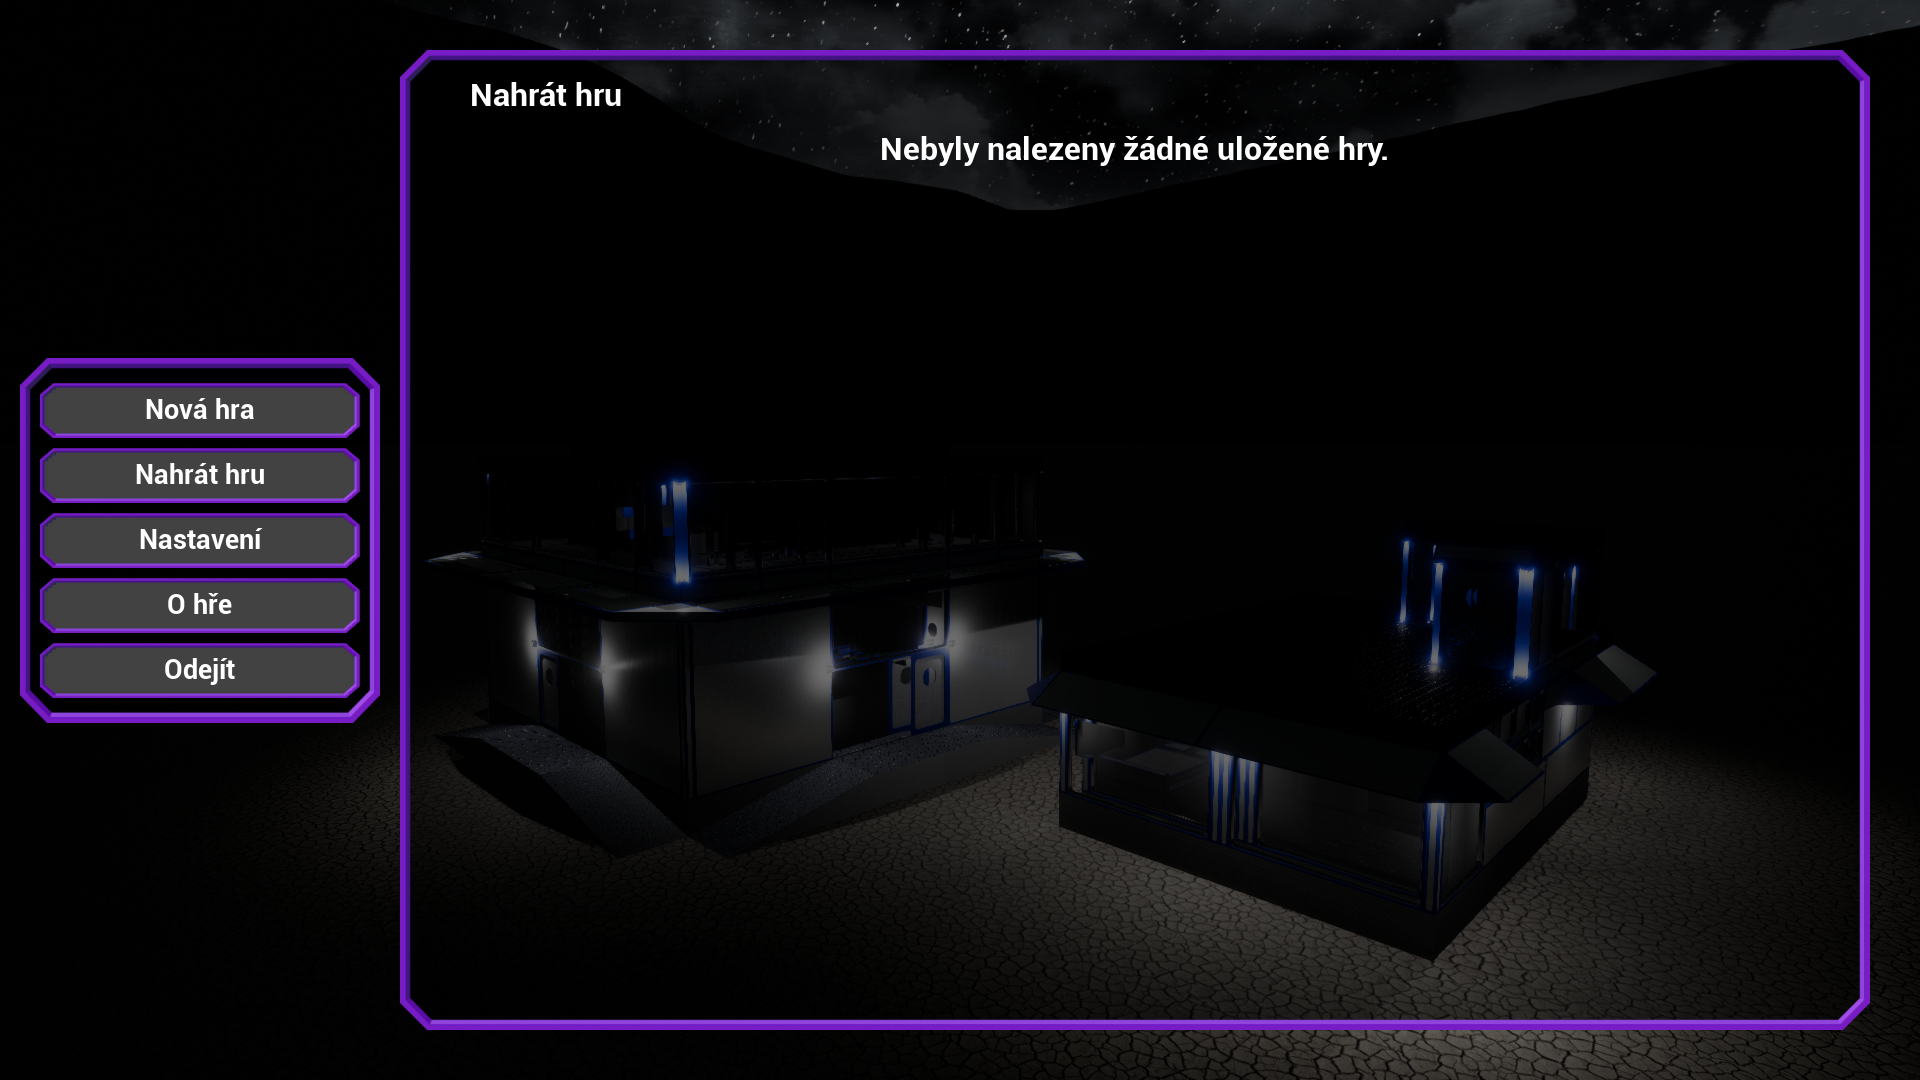
\includegraphics[ width=140mm]{../img/user/mainMenu/mmLoad}

\caption{Obrazovka hlavního menu -- Nahrát hru}
\label{fig:user_mainMenu_mmLoad}

\end{figure}
\FloatBarrier

Pod položkou \textbf{Nastavení} může uživatel měnit herní, zvuková a~grafická nastavení hry. Nastavení se aplikují a~ukládají okamžitě, výjimkou je pouze položka \textit{Animace generátoru energie}, která se projeví až po změně levelu. V~případě konfigurace z~hlavní nabídky se nastavení projeví okamžitě, v~případě konfigurace během rozehrané hry je potřeba vyvolat opětovné načtení uložené hry, nebo znovu spustit novou hru.

\begin{figure}[!ht]\centering
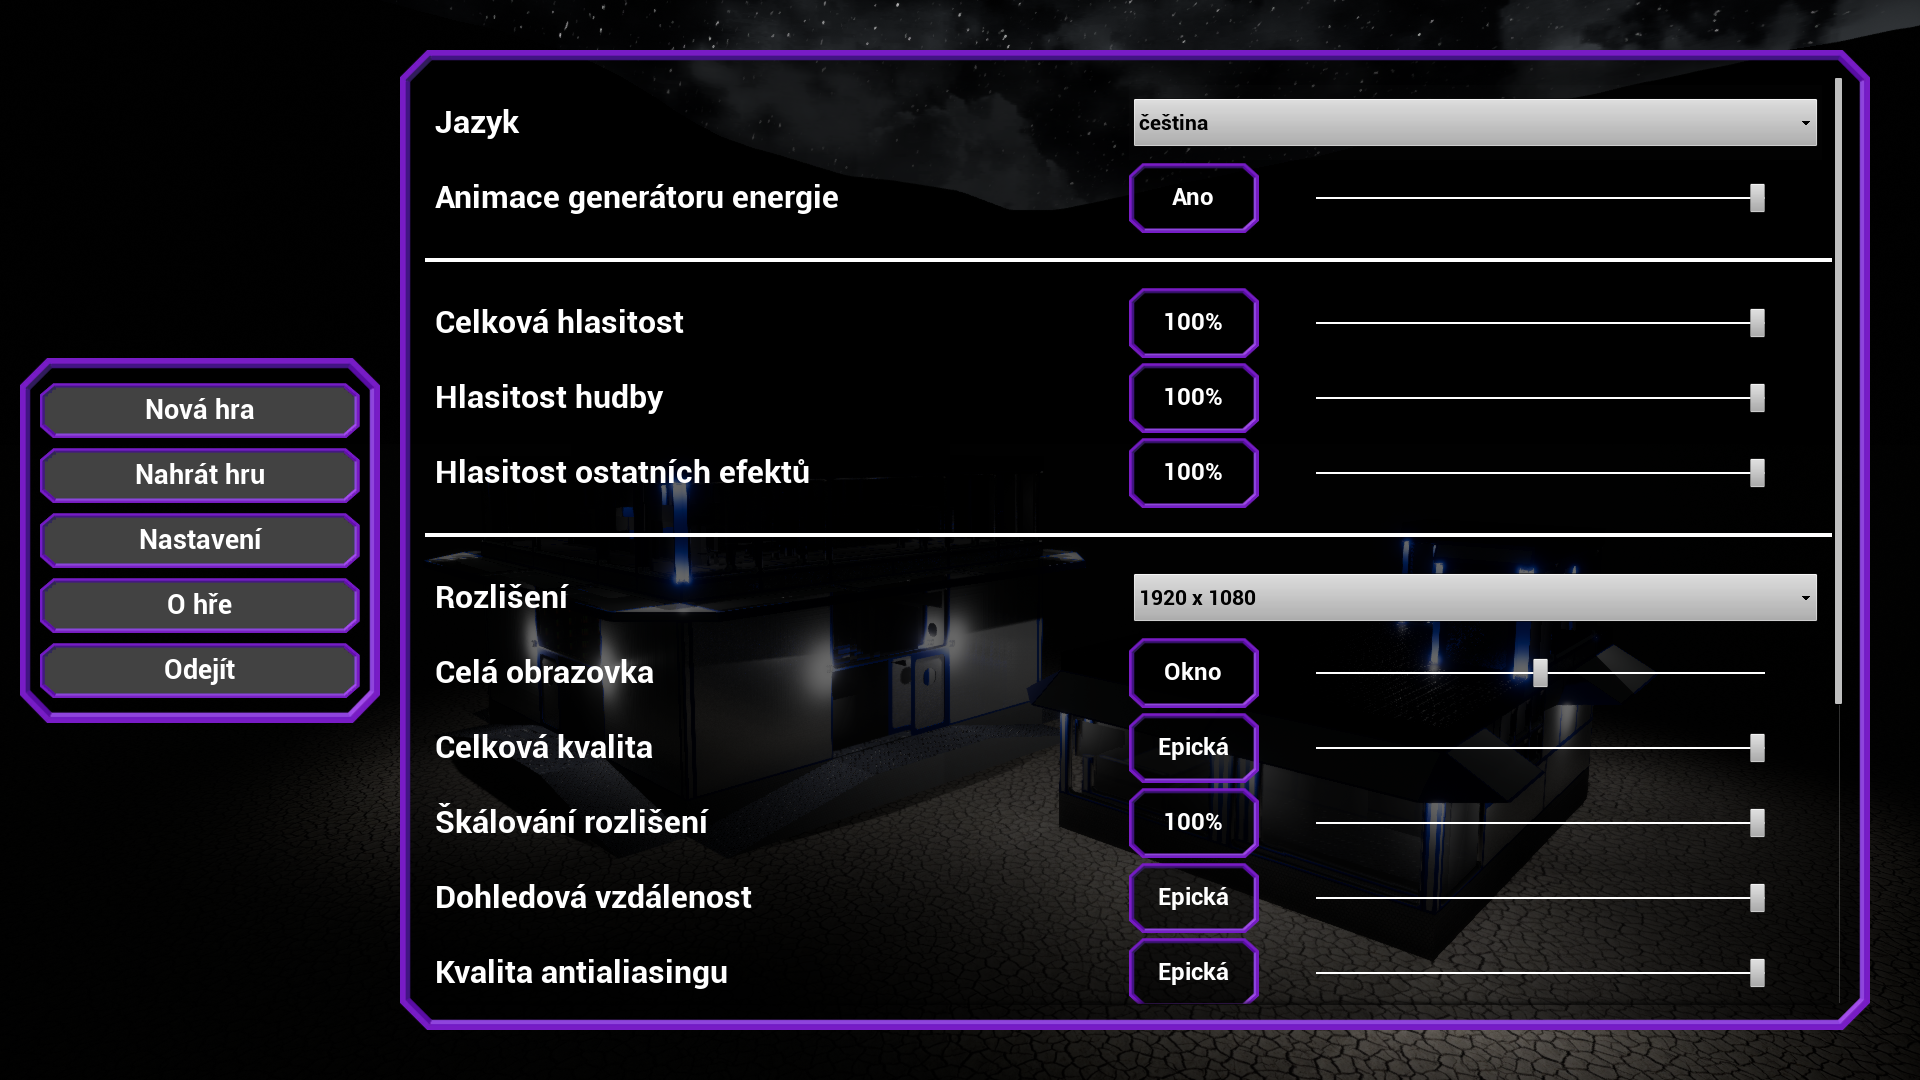
\includegraphics[ width=140mm]{../img/user/mainMenu/mmSettings}

\caption{Obrazovka hlavního menu -- Nastavení}
\label{fig:user_mainMenu_mmSettings}

\end{figure}

\FloatBarrier
%!TEX root = ../../prace.tex

\section{Herní menu - ukládání, nahrávání}

V průběhu rozehrané hry je možné použít \textbf{Rychlé uložení / načtení}, nebo si hru uložit z~herní nabídky.

Pro uložení hry je možné vytvořit nový save nebo přepsat stávající, pokud nějaký existuje. Uložené hry je též možné mazat.

\begin{figure}[!ht]\centering
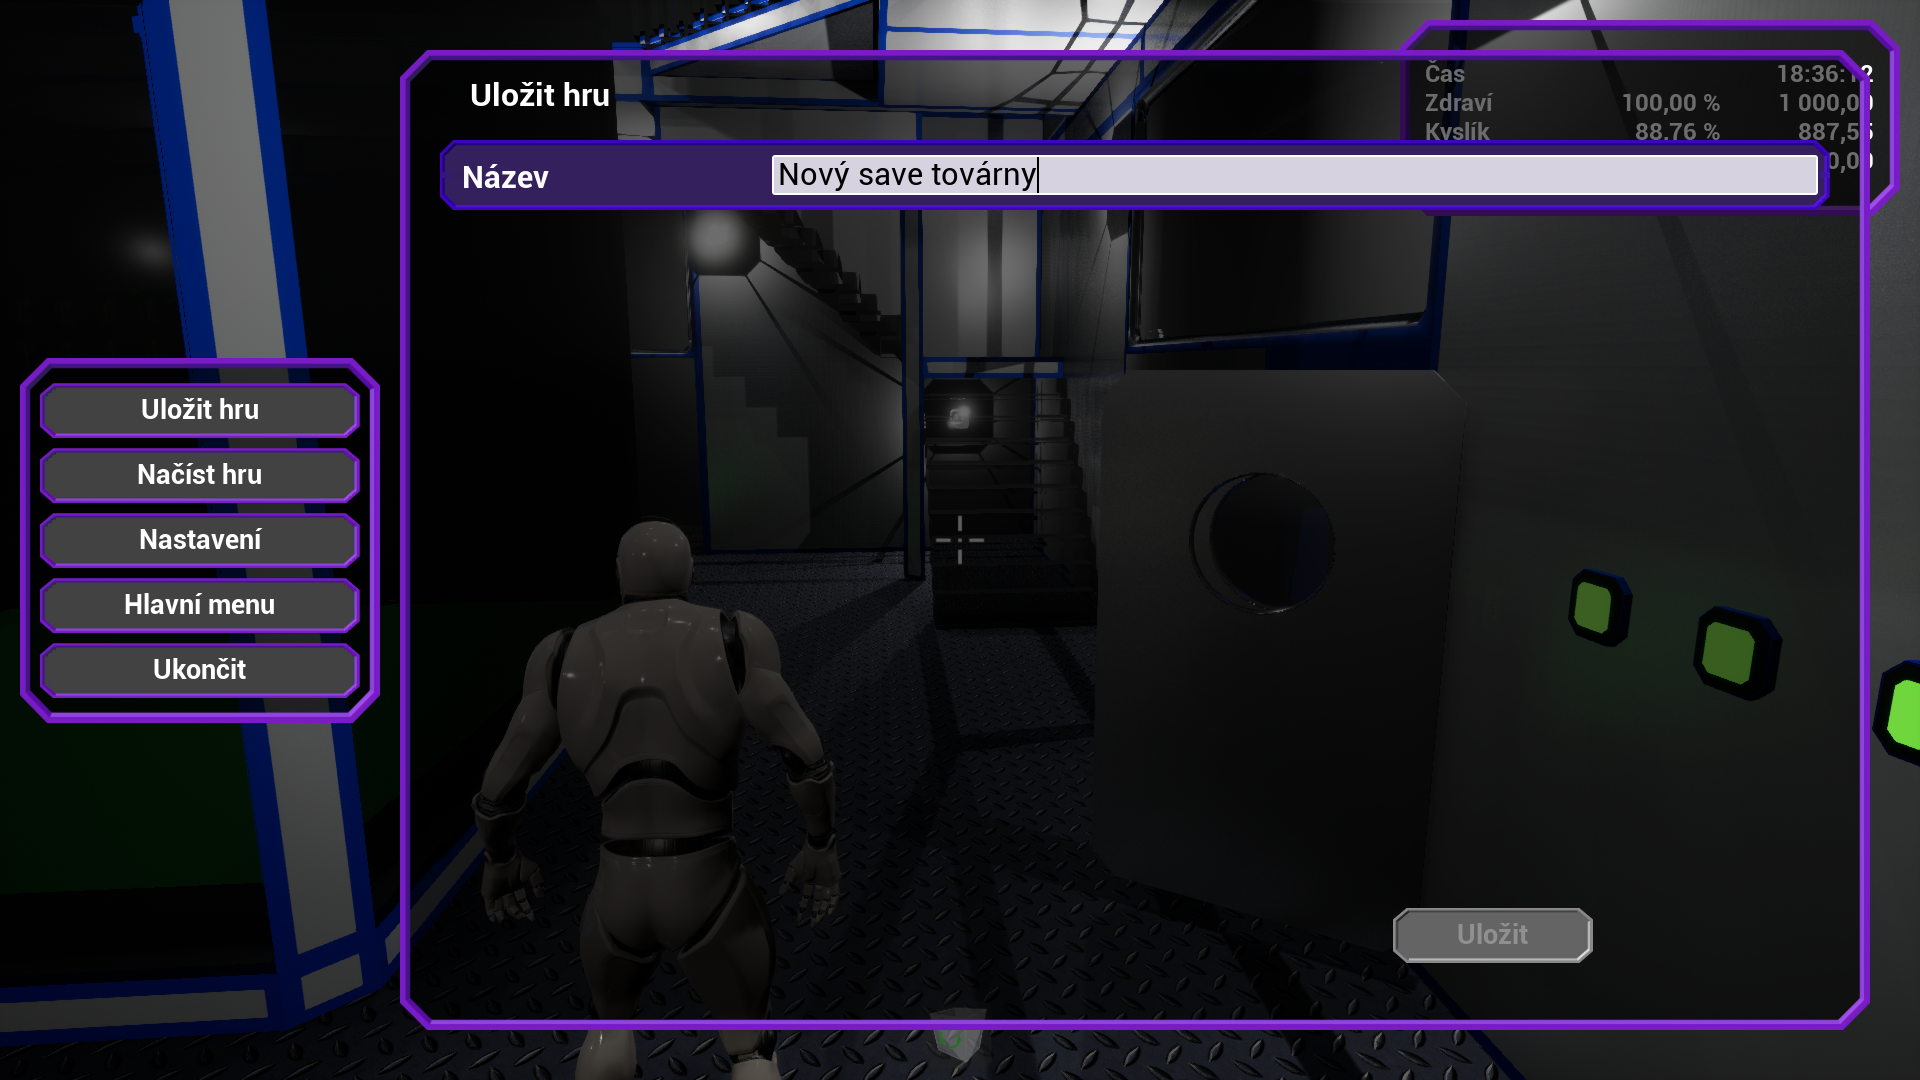
\includegraphics[ width=140mm]{../img/user/save/0newSave}

\caption{Ukládání - Nový save}
\label{fig:user_save_0newSave}

\end{figure}
\FloatBarrier

Pokud bylo uložení úspěšné, hráči se zobrazí následující hláška:

\begin{figure}[!ht]\centering
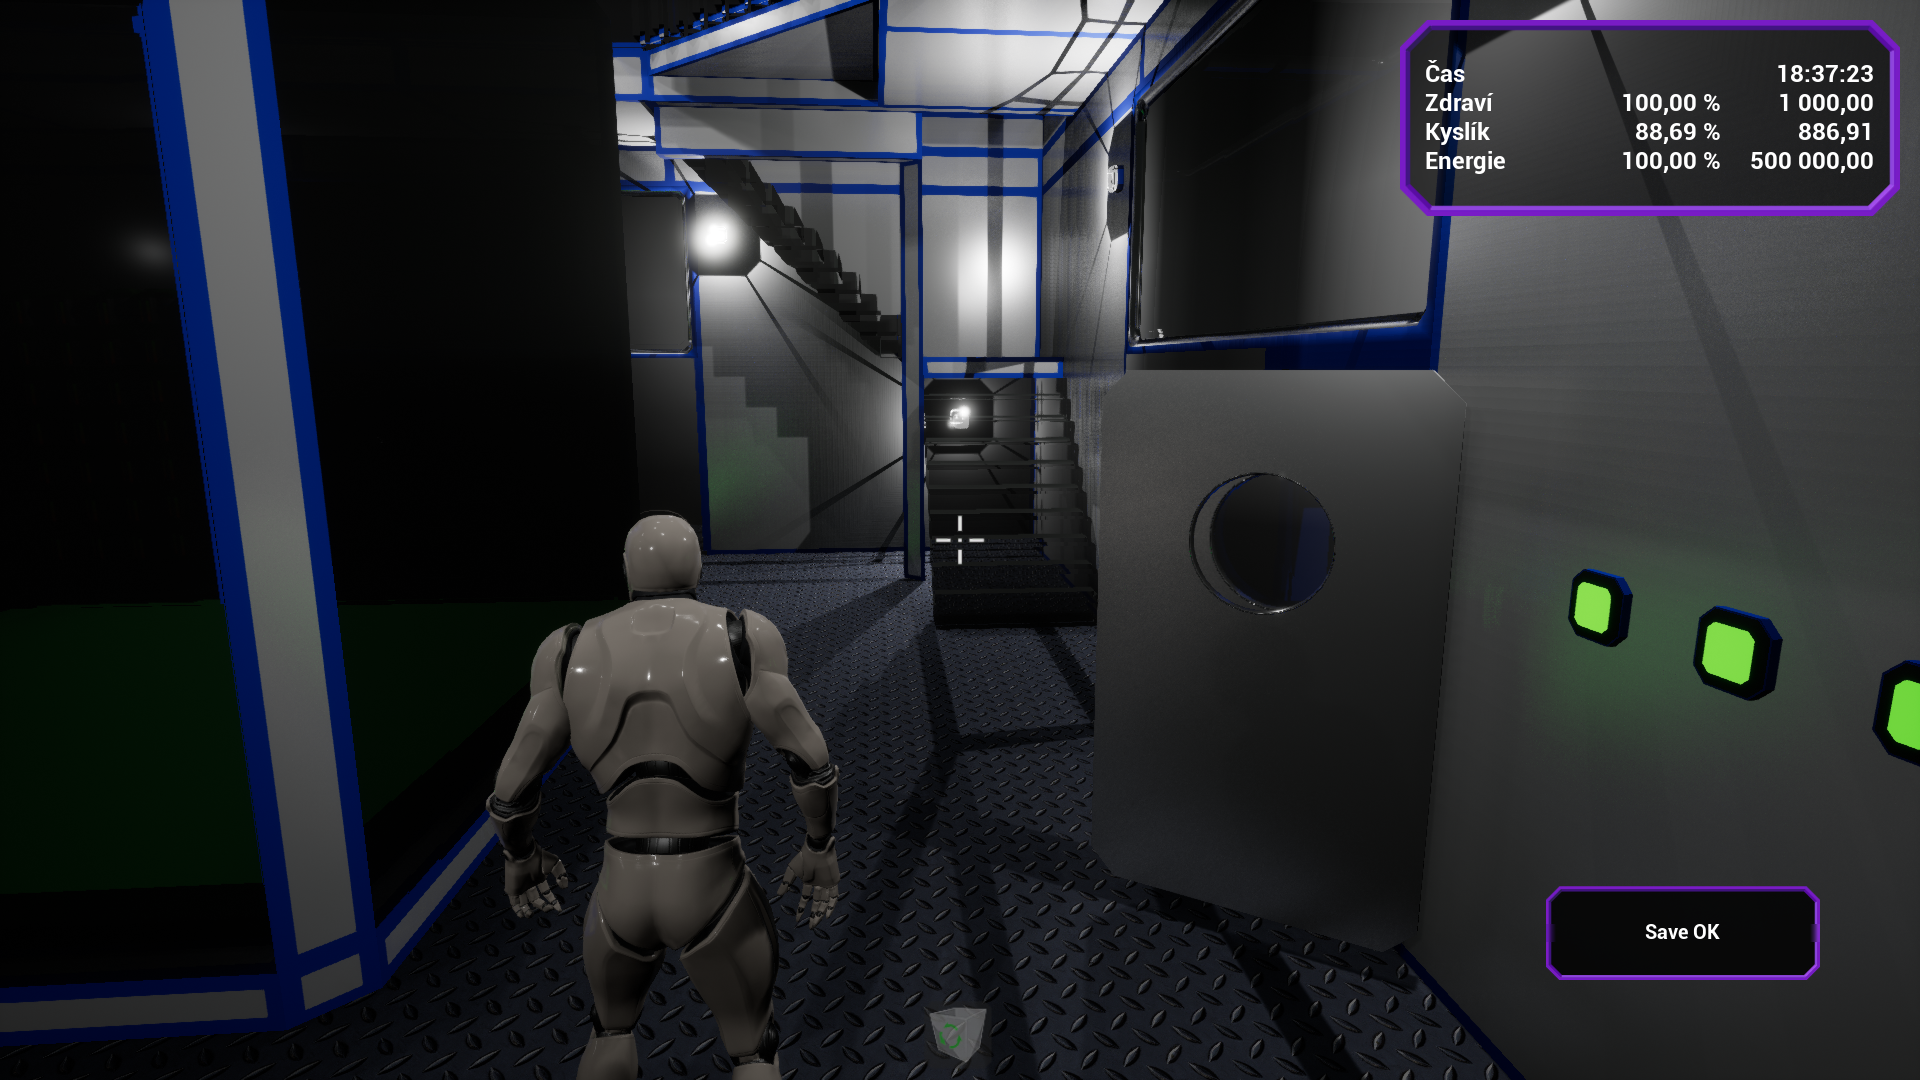
\includegraphics[ width=140mm]{../img/user/save/1afterSave}

\caption{Ukládání - po uložení}
\label{fig:user_save_1afterSave}

\end{figure}
\FloatBarrier

Nahrávat je možné ze všech uložených pozic, včetně rychlého uložení. Opět je zde možné vybraný save smazat.

\begin{figure}[!ht]\centering
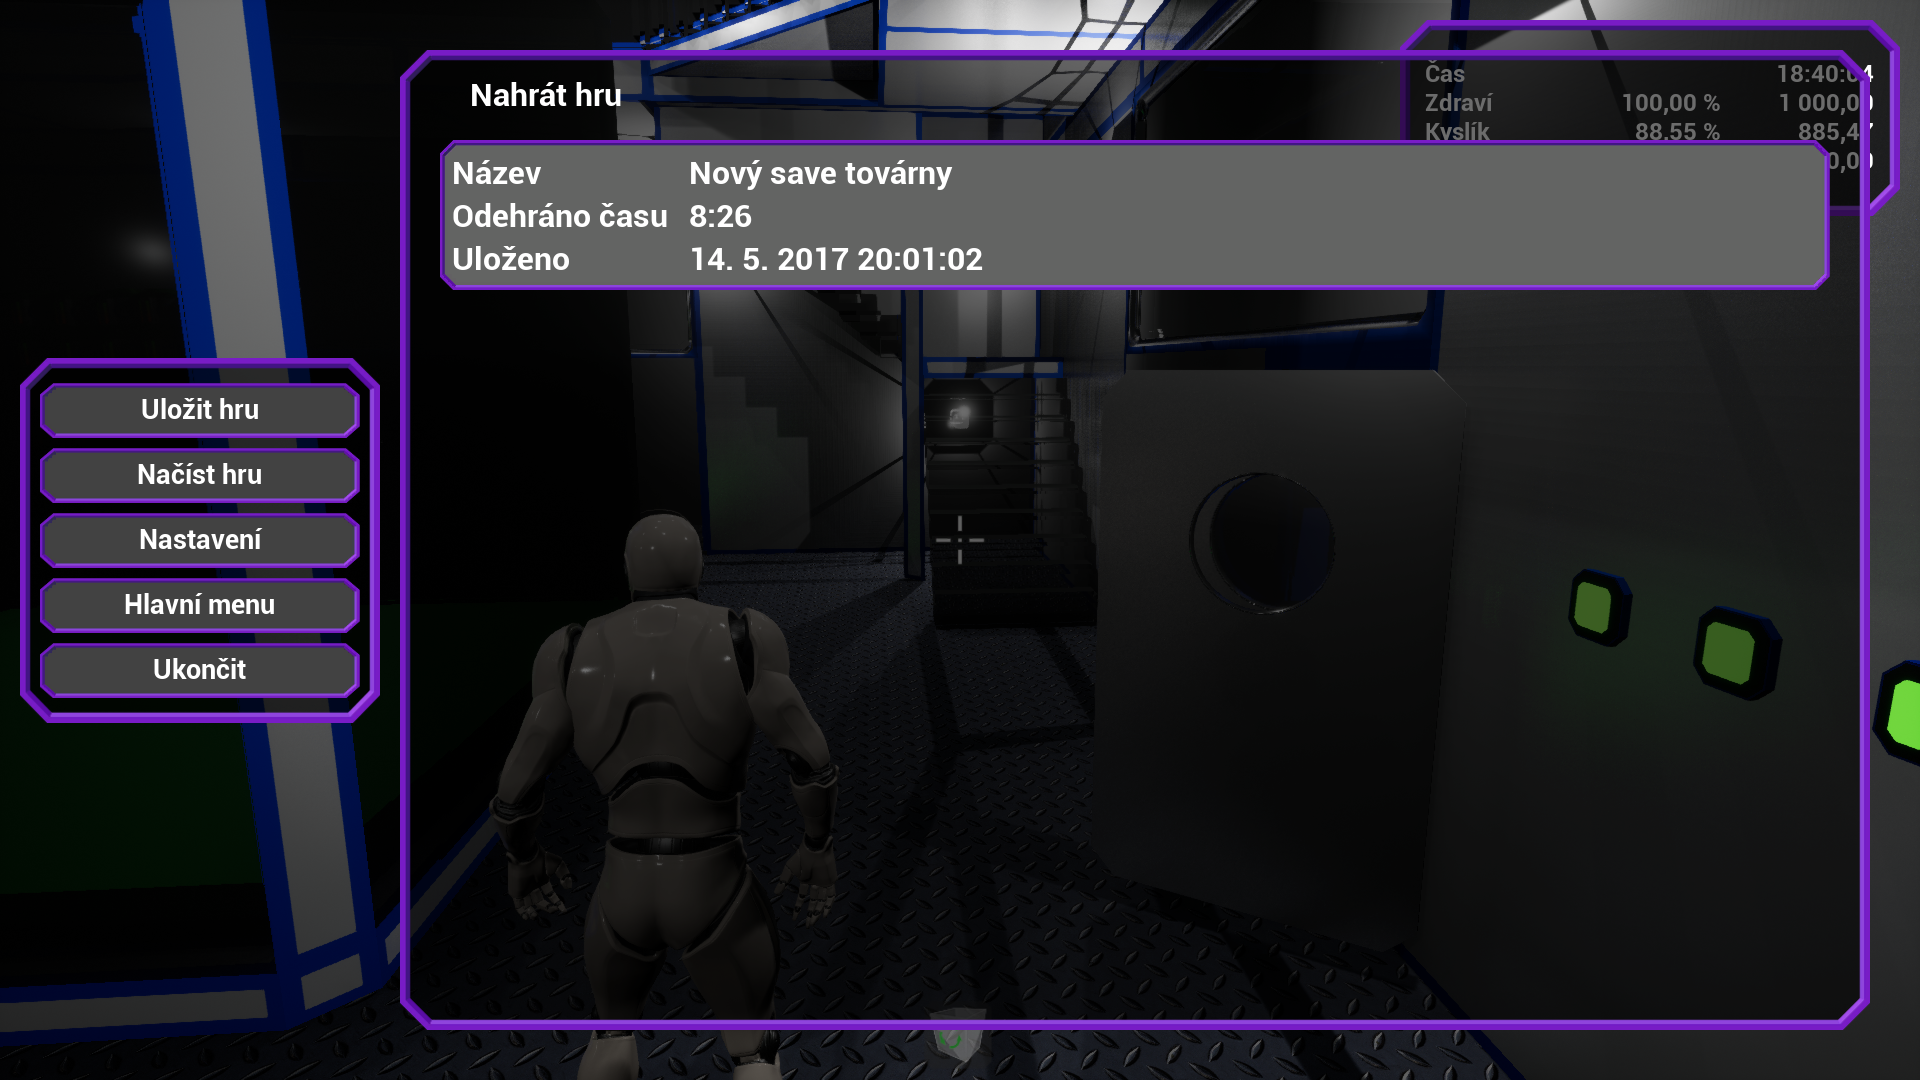
\includegraphics[ width=140mm]{../img/user/save/2load}

\caption{Ukládání - nahrát hru}
\label{fig:user_save_2load}

\end{figure}
\FloatBarrier

Pokud má hráč rozehranou hru, je pro jistotu vyžadováno potvrzení.

\begin{figure}[!ht]\centering
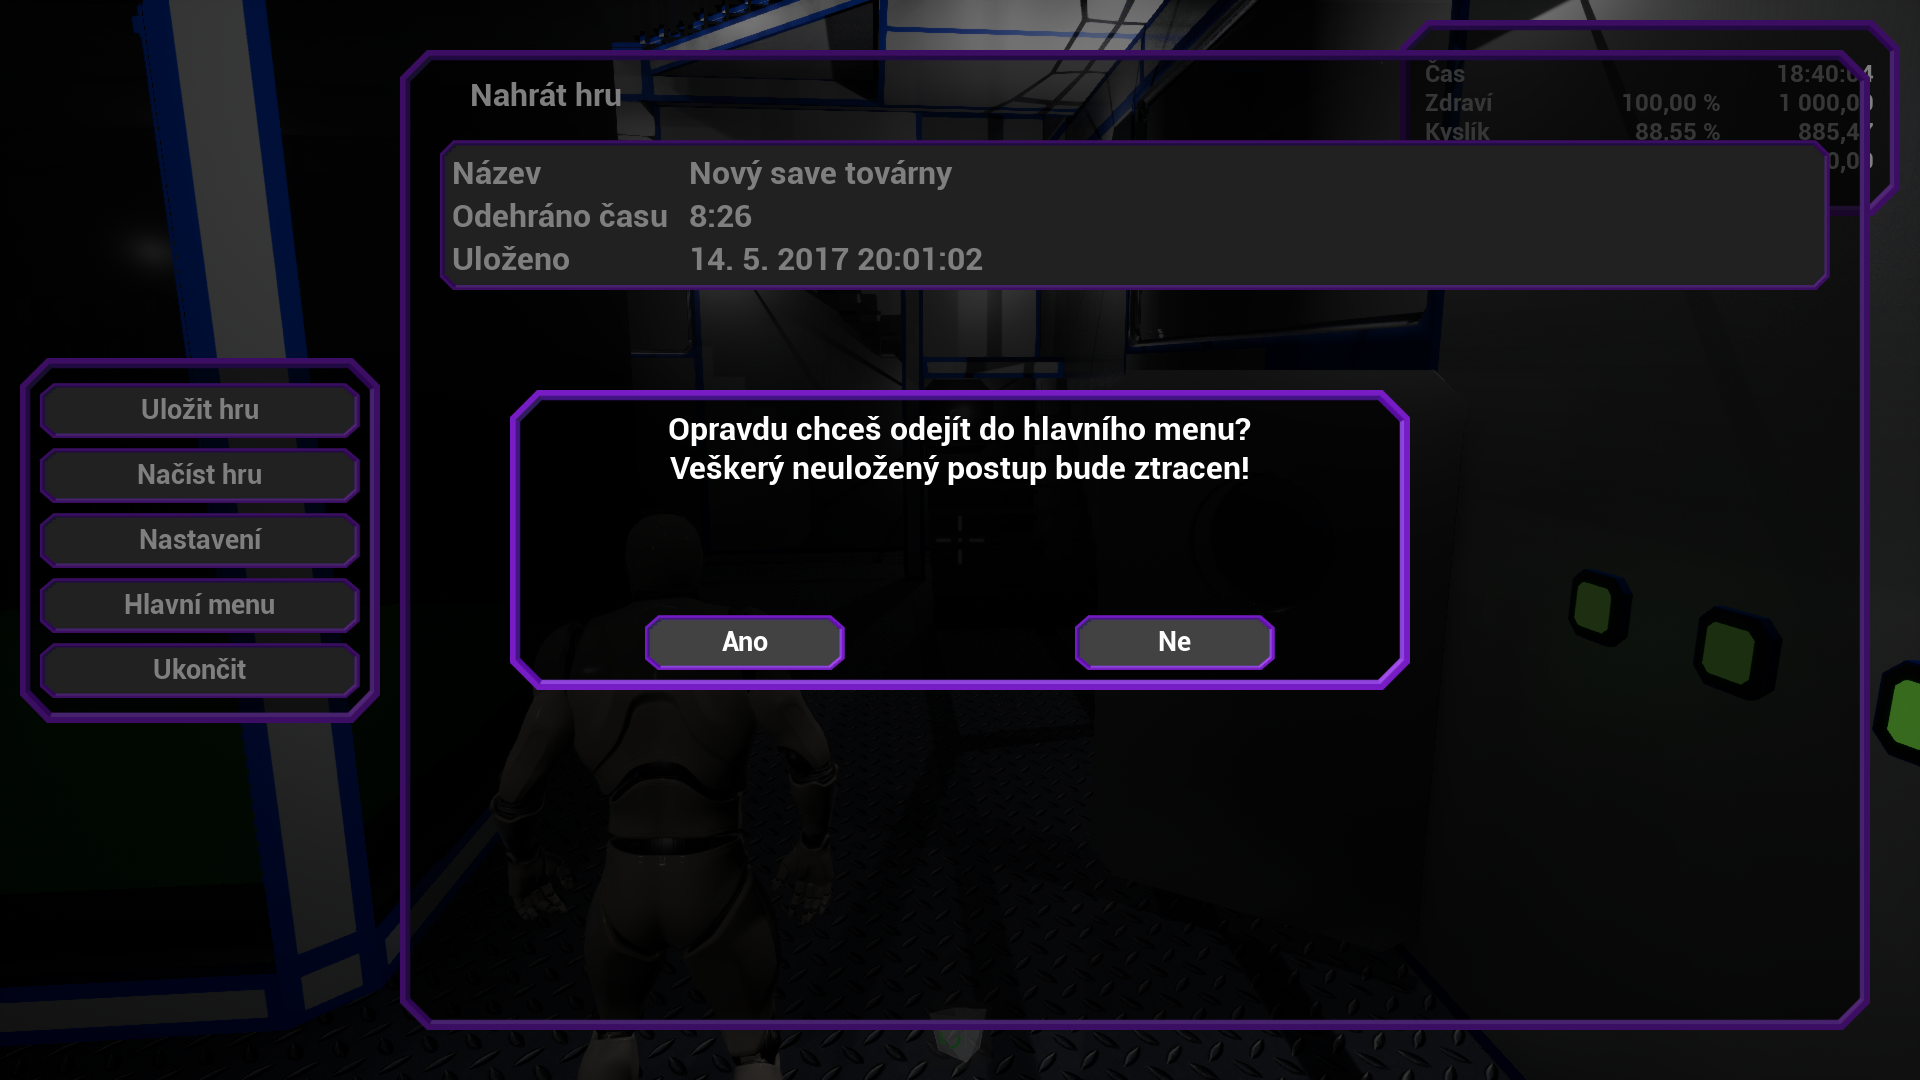
\includegraphics[ width=140mm]{../img/user/save/3loadClicked}

\caption{Ukládání - potvrzení nahrání hry}
\label{fig:user_save_3loadClicked}

\end{figure}

\FloatBarrier
%!TEX root = ../../prace.tex

\section{Inventář}

Inventář se vyvolá klávesou \textbf{E}. Zobrazí se následující obrazovka:

\begin{figure}[!ht]\centering
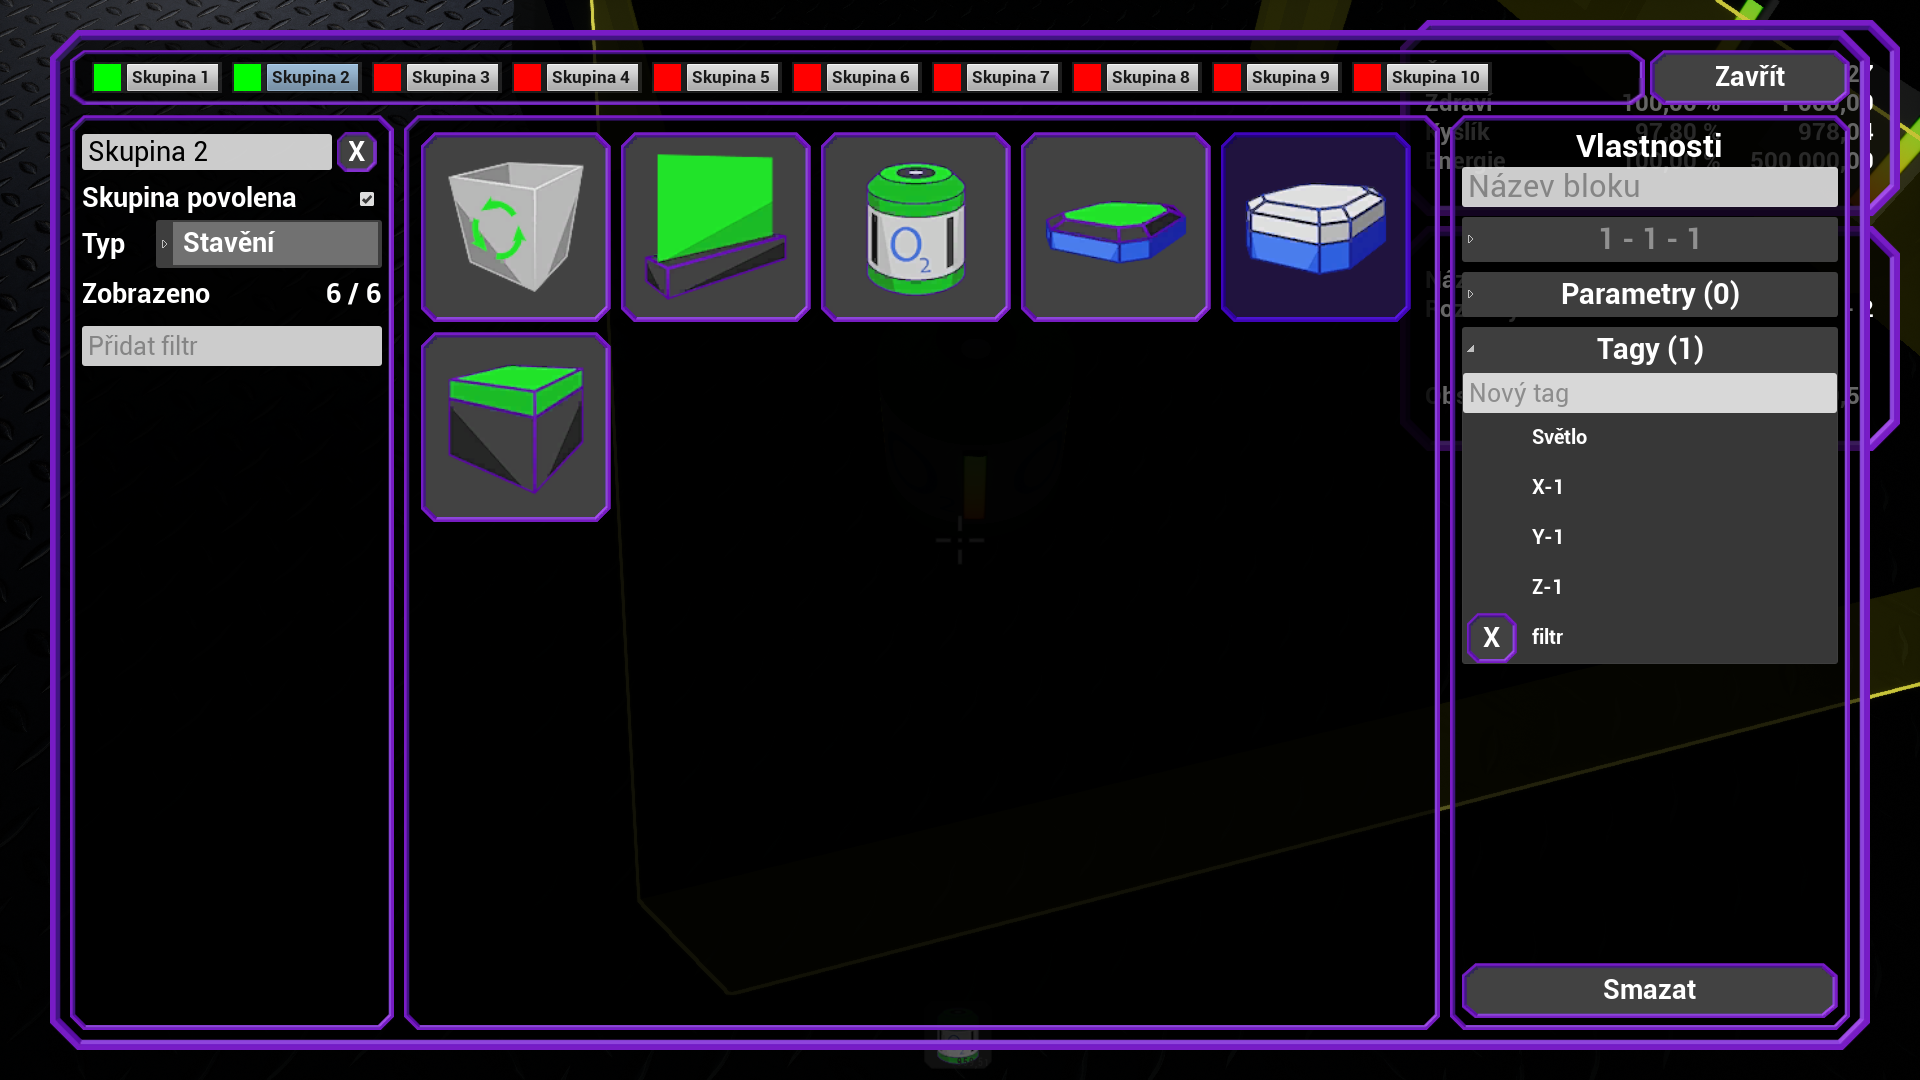
\includegraphics[ width=140mm]{../img/user/inventory/0AddTag}

\caption{Inventář - přehled}
\label{fig:user_inventory_0AddTag}

\end{figure}

\FloatBarrier

V horní části je výběr skupin. Je možné vybírat z 10 skupin, které si lze pojmenovat dle libosti. Dále je možné je (de)aktivovat buď kliknutím na zelený / červený čtverec, nebo skrze příslušný checkbox v editaci skupiny.
Je možné používat standardní změnu skupiny klávesami \textbf{ú} a \textbf{)}, editační okno se pak příslušným způsobem změní. 

V \textit{levé} části je \textbf{editor skupiny}, jehož funkce budou popsány v textu dále. \textit{Uprostřed} je možné vidět postavitelné či umístitelné položky, které jsou dofiltrovány dle právě nastaveného filtru. Výběrem položky lze editovat její vlastnosti v \textit{pravé} části okna

\FloatBarrier

Každá skupina umožňuje definovat své filtry. Matematicky bychom mohli popsat filtrování jako vyhodnocení formule v \textit{CNF}. Pokud do pole \textit{Přidat filtr} napíšeme tagy oddělené mezerou, do skupiny se přidá \textbf{nová} skupina s výchozím pojmenováním.

\begin{figure}[!ht]\centering
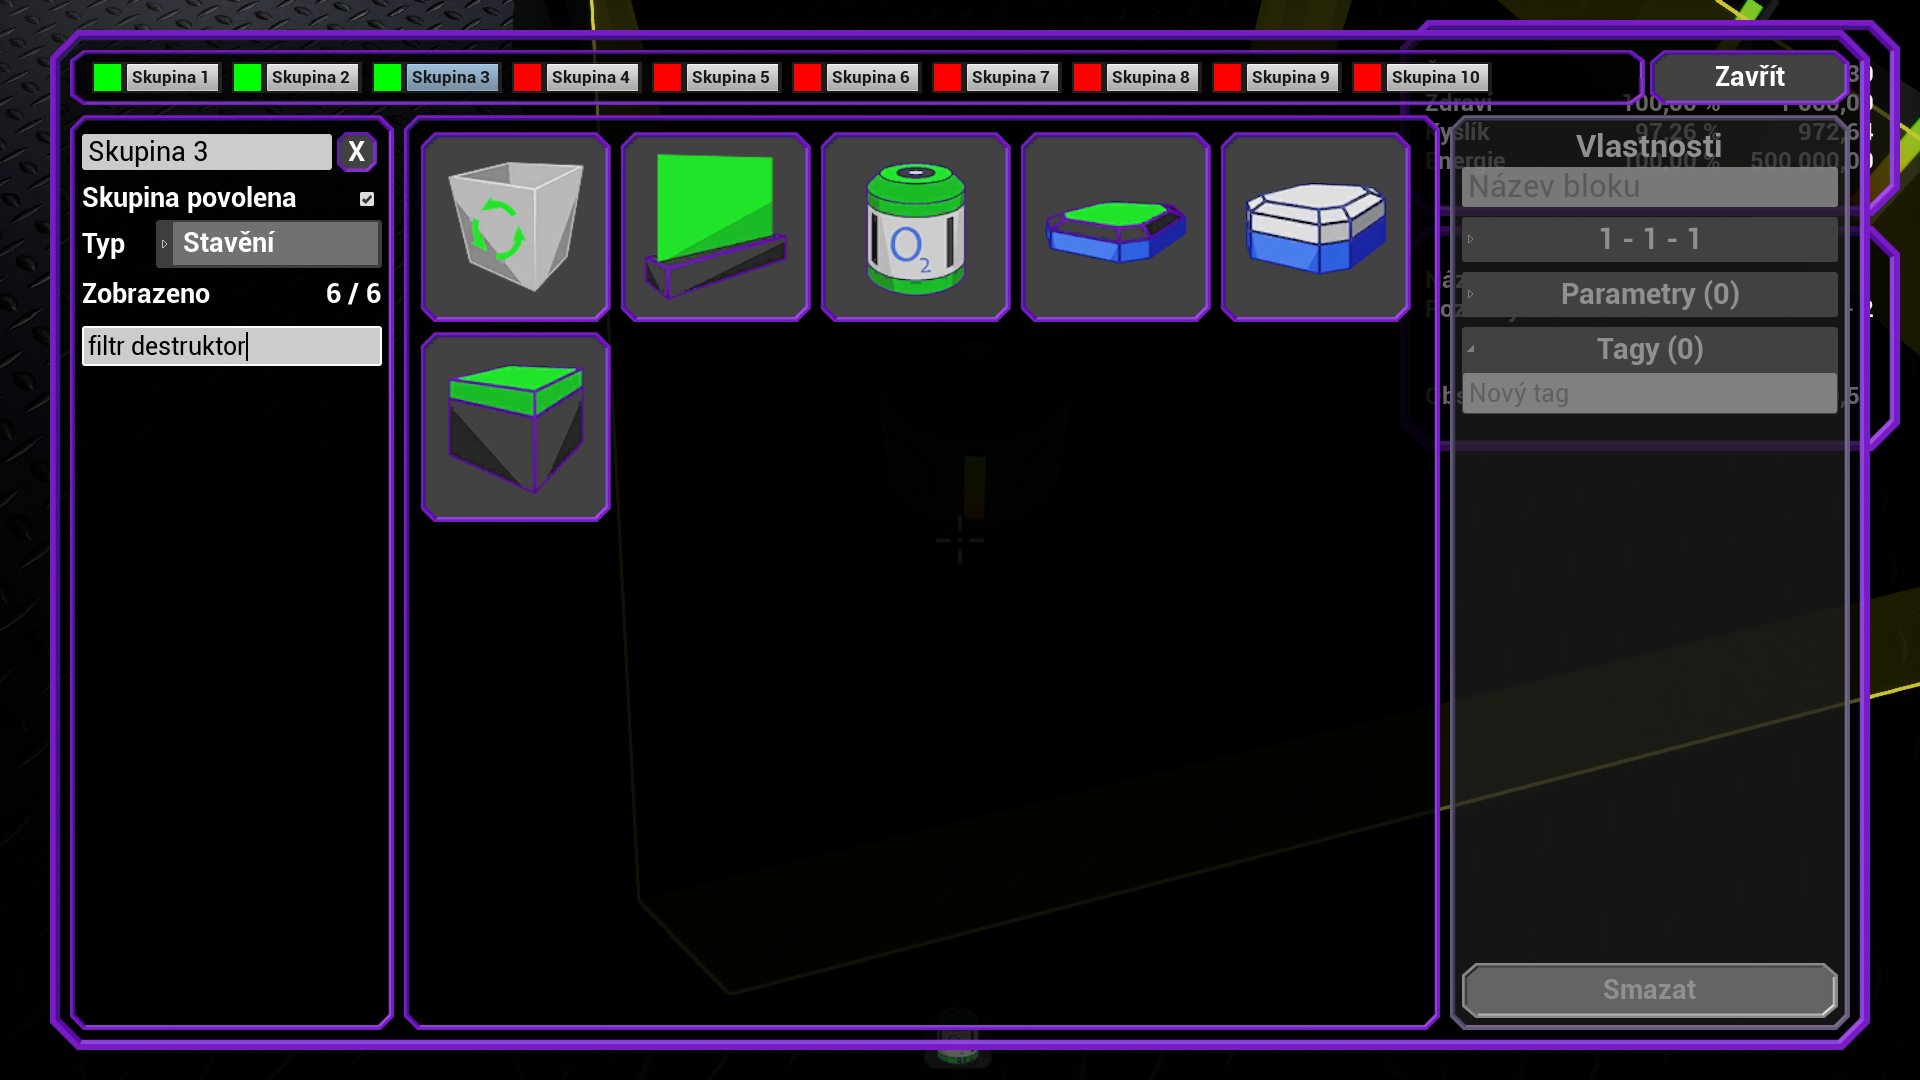
\includegraphics[ width=140mm]{../img/user/inventory/1setFilter}

\caption{Inventář - přidání skupiny}
\label{fig:user_inventory_1setFilter}

\end{figure}

\FloatBarrier

Po přidání se seznam dostupných prvků dofiltruje podle nastavených tagů - ve výsledku bude každá položka splňovat alespoň jeden tag z každé skupiny. Shoda nemusí být přesná, tag objektu musí obsahovat podřetězec definovaný filtrem.
\begin{figure}[!ht]\centering
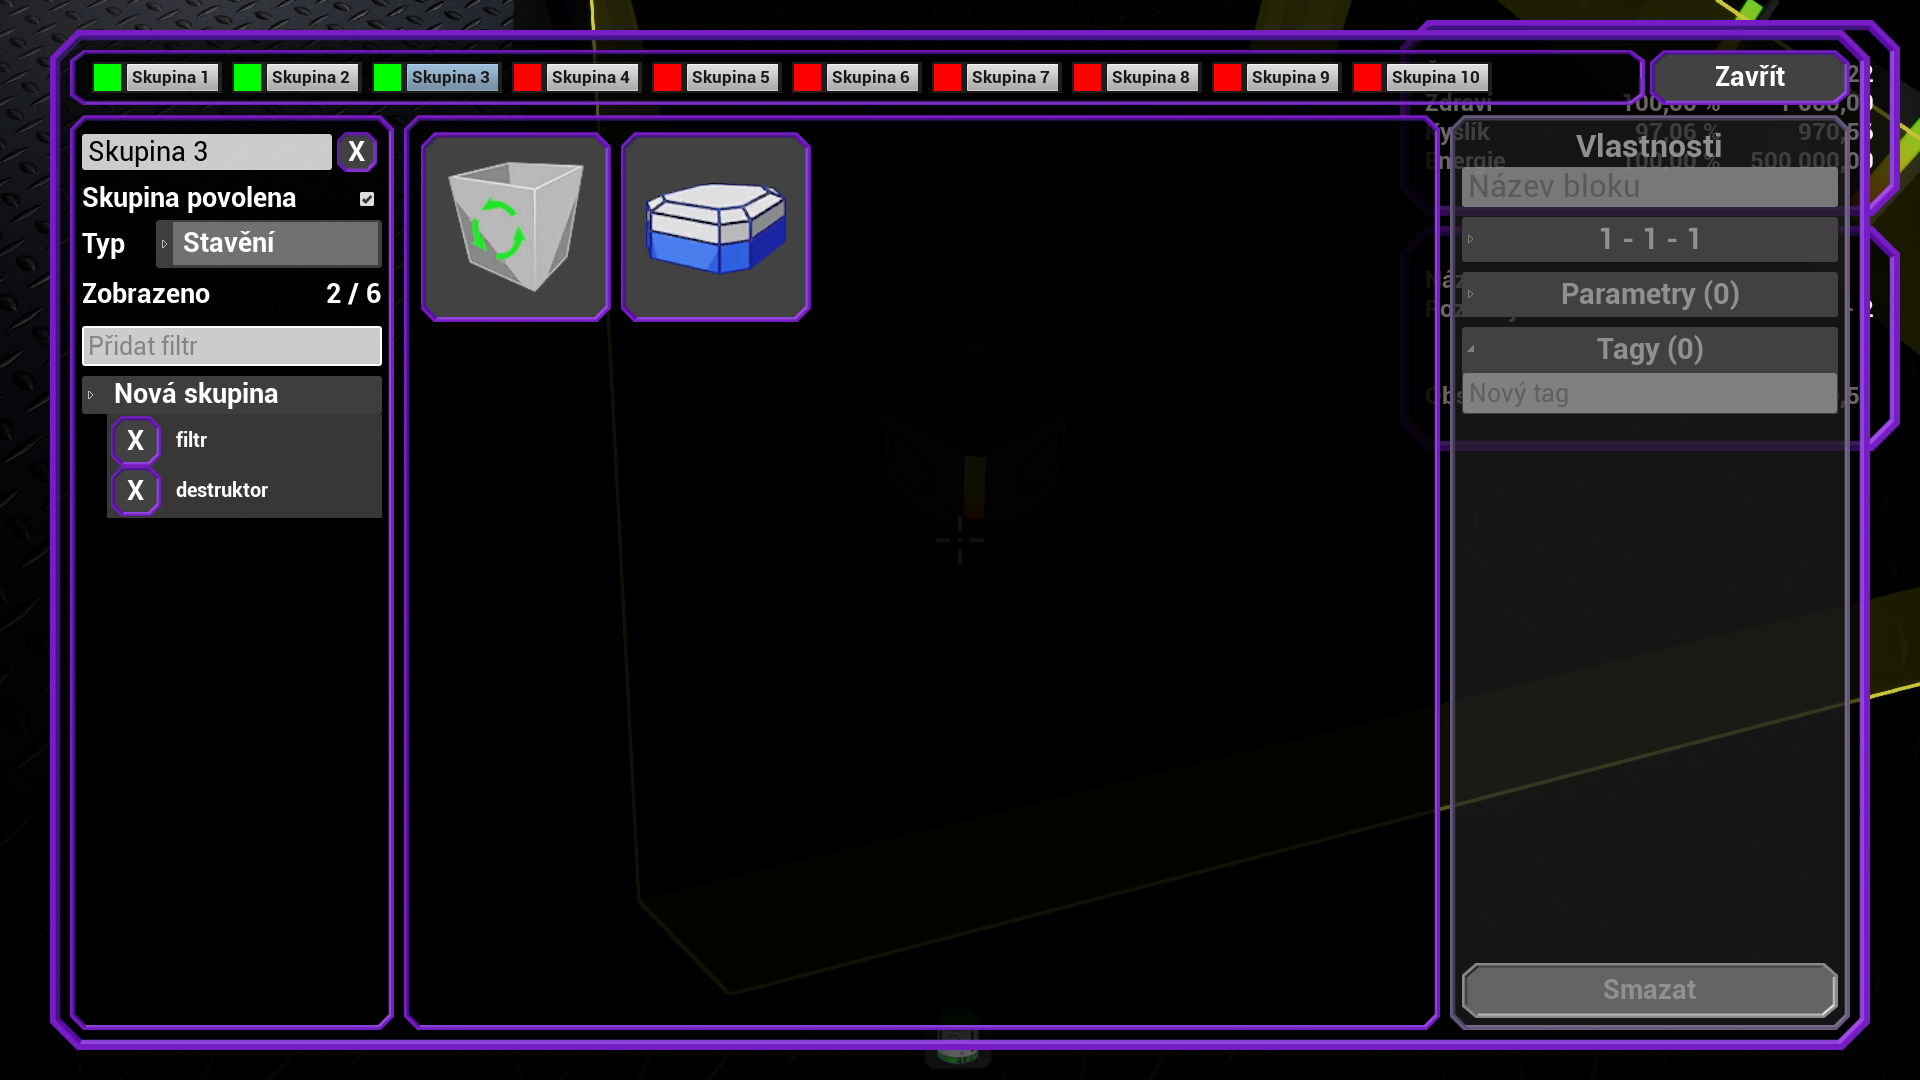
\includegraphics[ width=140mm]{../img/user/inventory/2filterResult}

\caption{Inventář - výsledek s filtrovanými položkami}
\label{fig:user_inventory_2filterResult}

\end{figure}

\FloatBarrier

Na následujícím obrázku je možné vidět filtry s rozbalenými vlastnostmi. Zaměřme se nyní na část \textit{Nesbalovat}. Po zaškrtnutí této volby je zobrazena pouze hlavička skupiny.

\begin{figure}[!ht]\centering
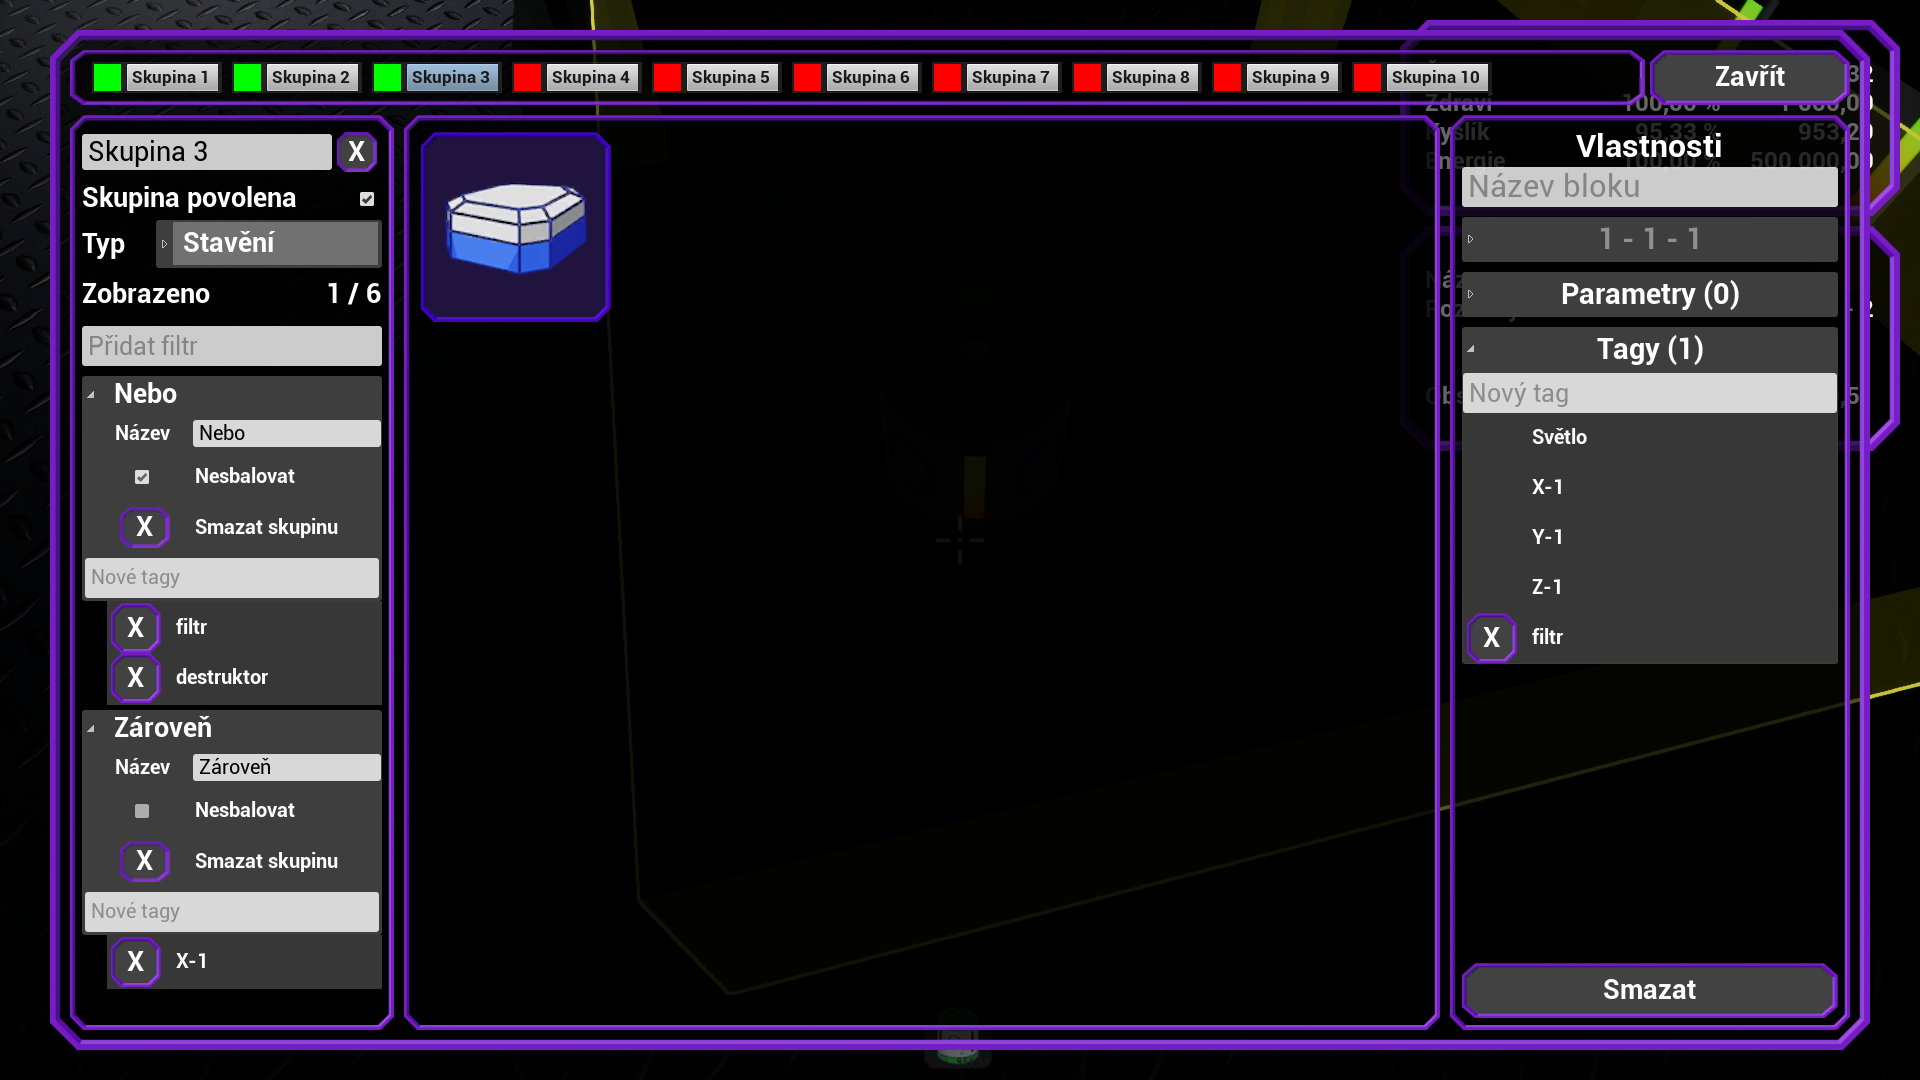
\includegraphics[ width=140mm]{../img/user/inventory/3additionalFilter}

\caption{Inventář - Nová hra}
\label{fig:user_inventory_3additionalFilter}

\end{figure}

\FloatBarrier

Výsledný seznam se sbalenými vlastnostmi filtru:

\begin{figure}[!ht]\centering
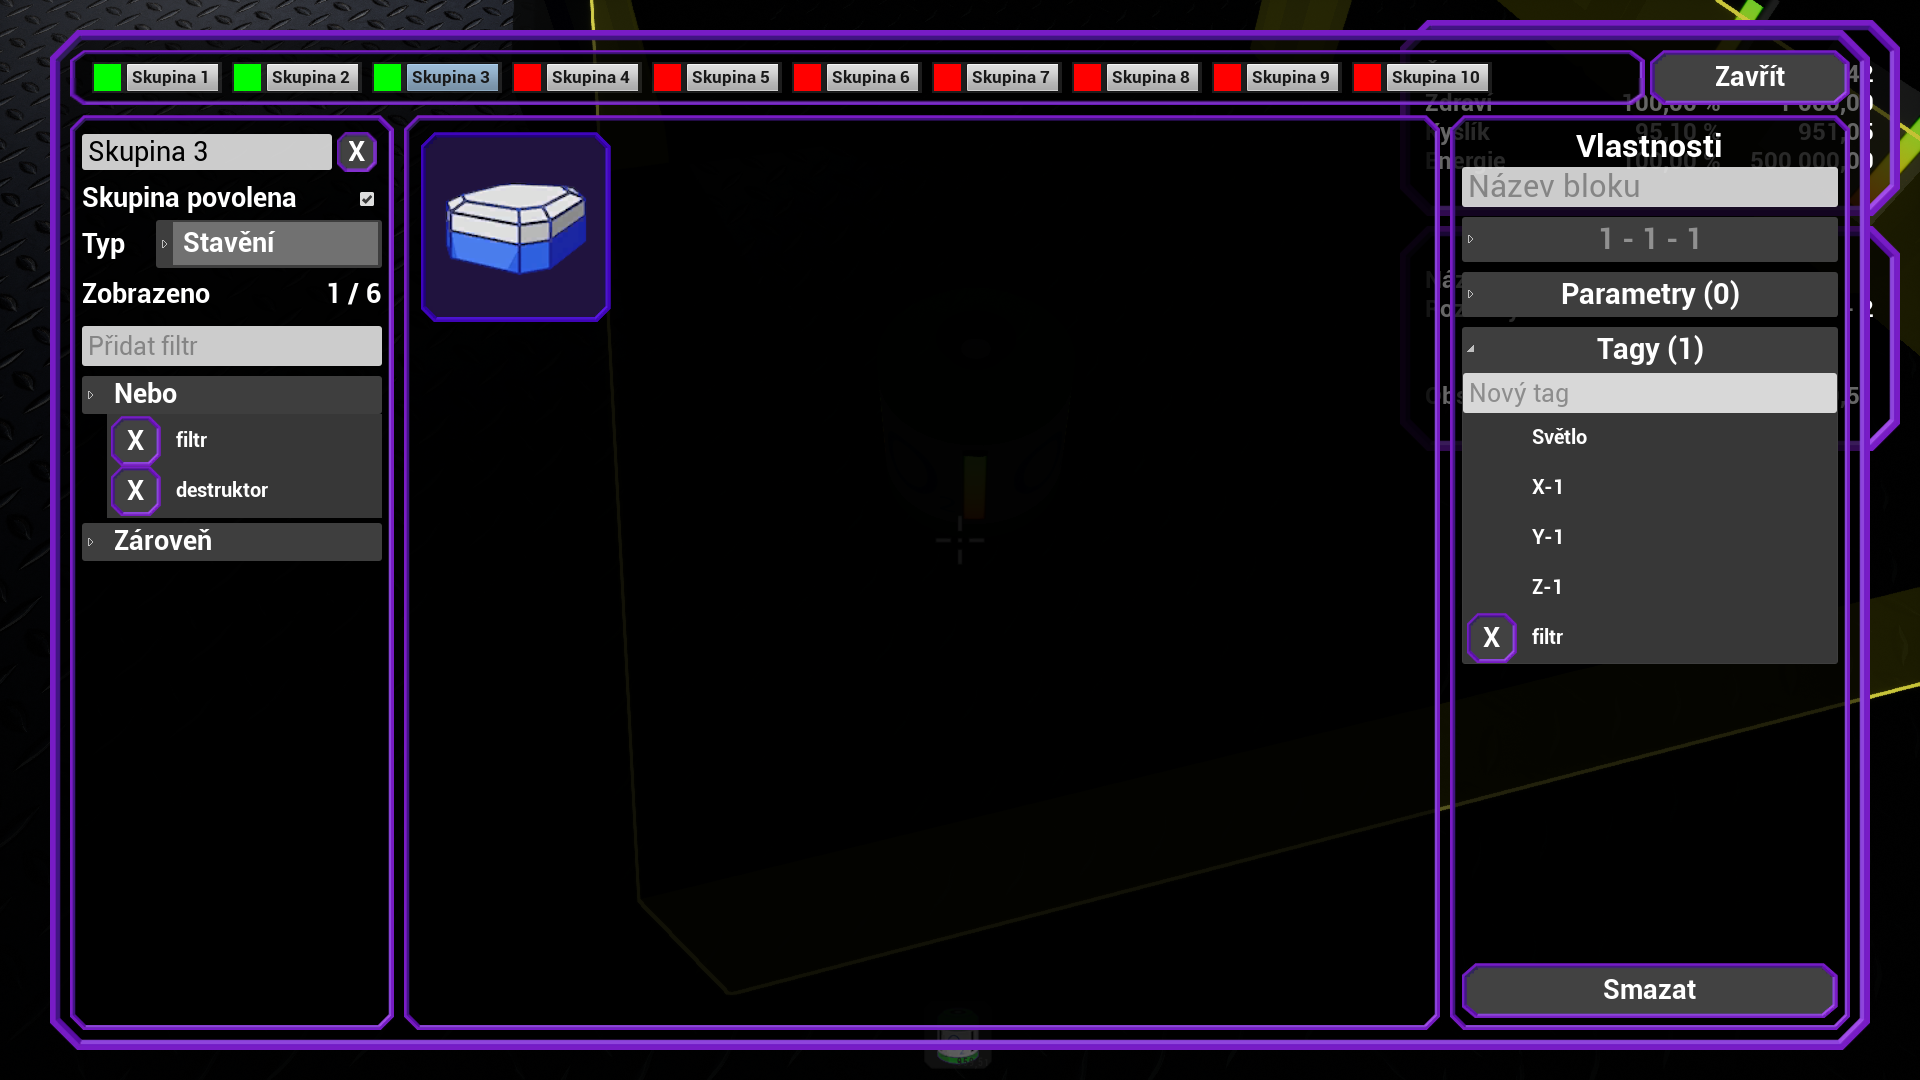
\includegraphics[ width=140mm]{../img/user/inventory/4addFilterCollapsed}

\caption{Inventář - Nahrát hru}
\label{fig:user_inventory_4addFilterCollapsed}

\end{figure}

\FloatBarrier

Označené položky je také možné smazat z inventáře. Umístitelné položky tak mohou být reálně zničeny. 

\begin{figure}[!ht]\centering
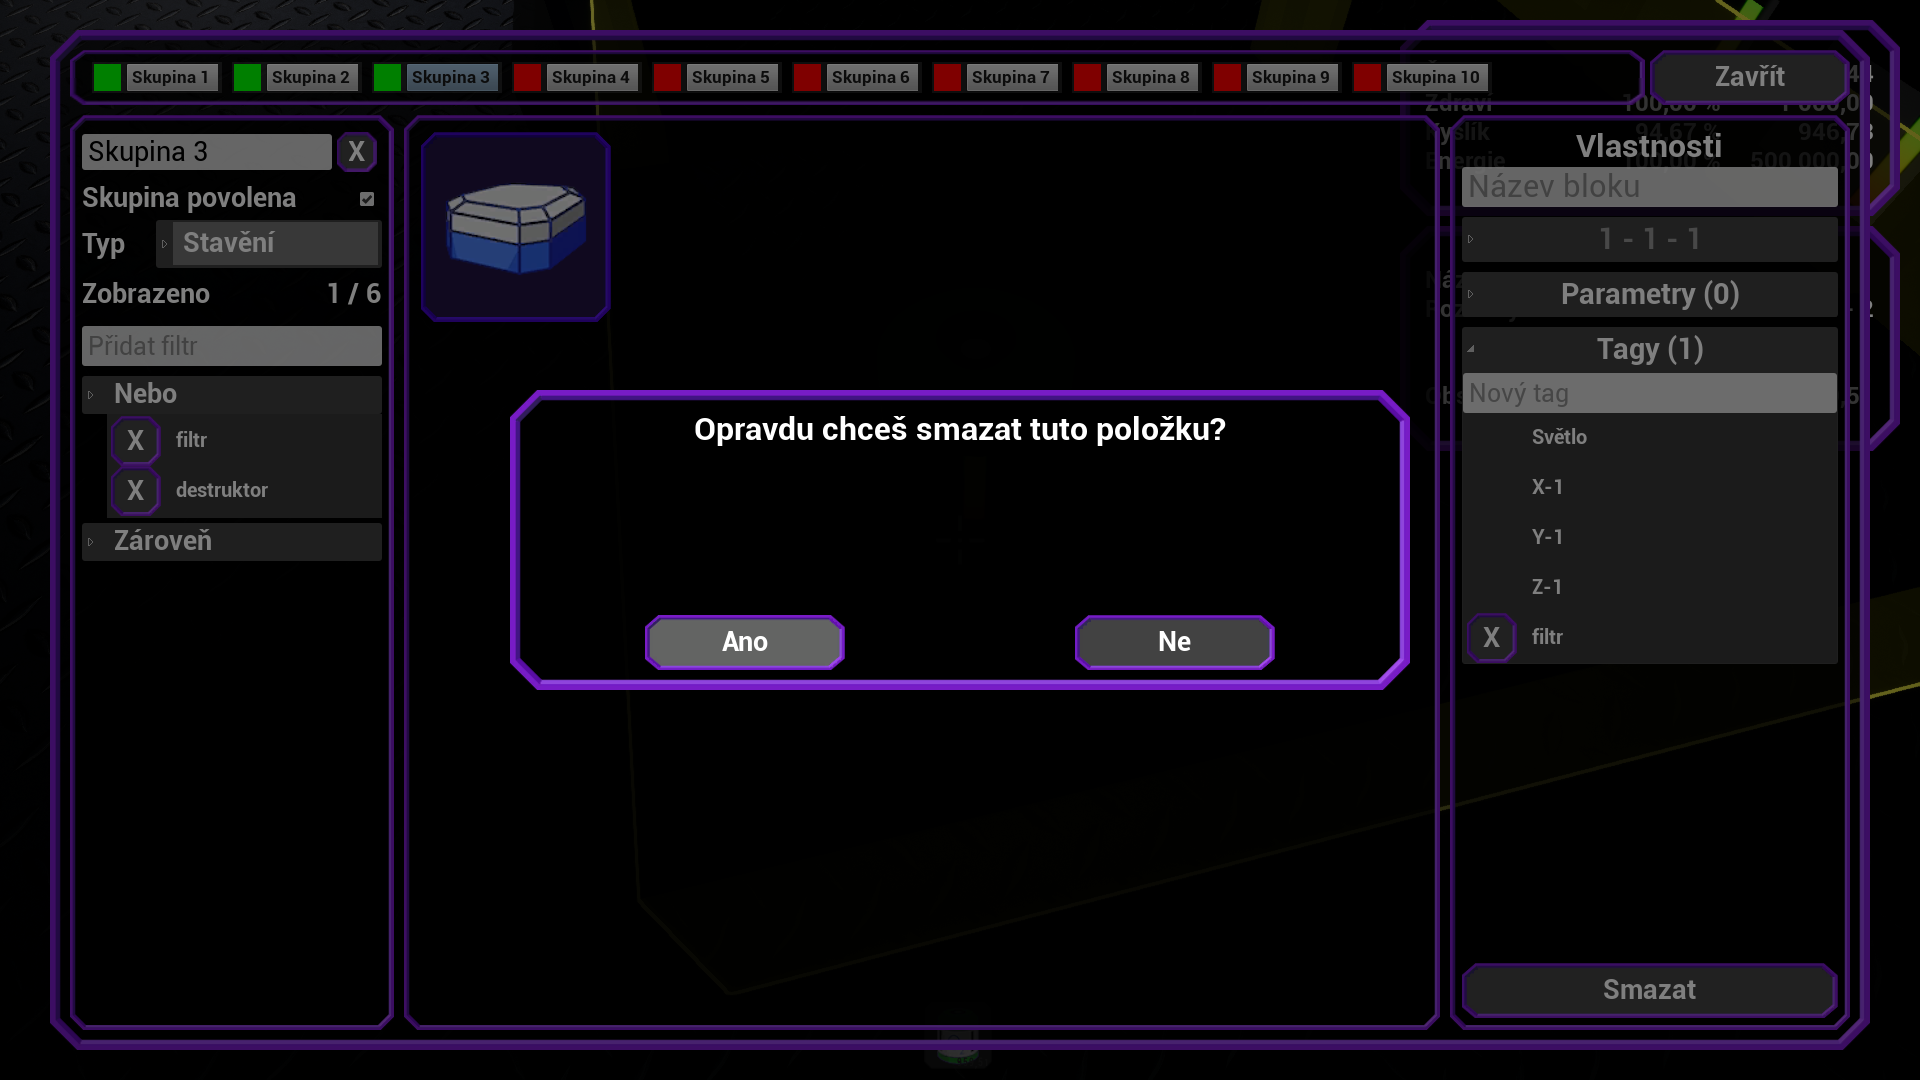
\includegraphics[ width=140mm]{../img/user/inventory/5deleteItem}

\caption{Inventář - Nastavení}
\label{fig:user_inventory_5deleteItem}

\end{figure}

\FloatBarrier
V případě, že je zvolena položka s dodatečnými parametry, je možné jejich hodnoty vidět v editoru vlastností bloku

\begin{figure}[!ht]\centering
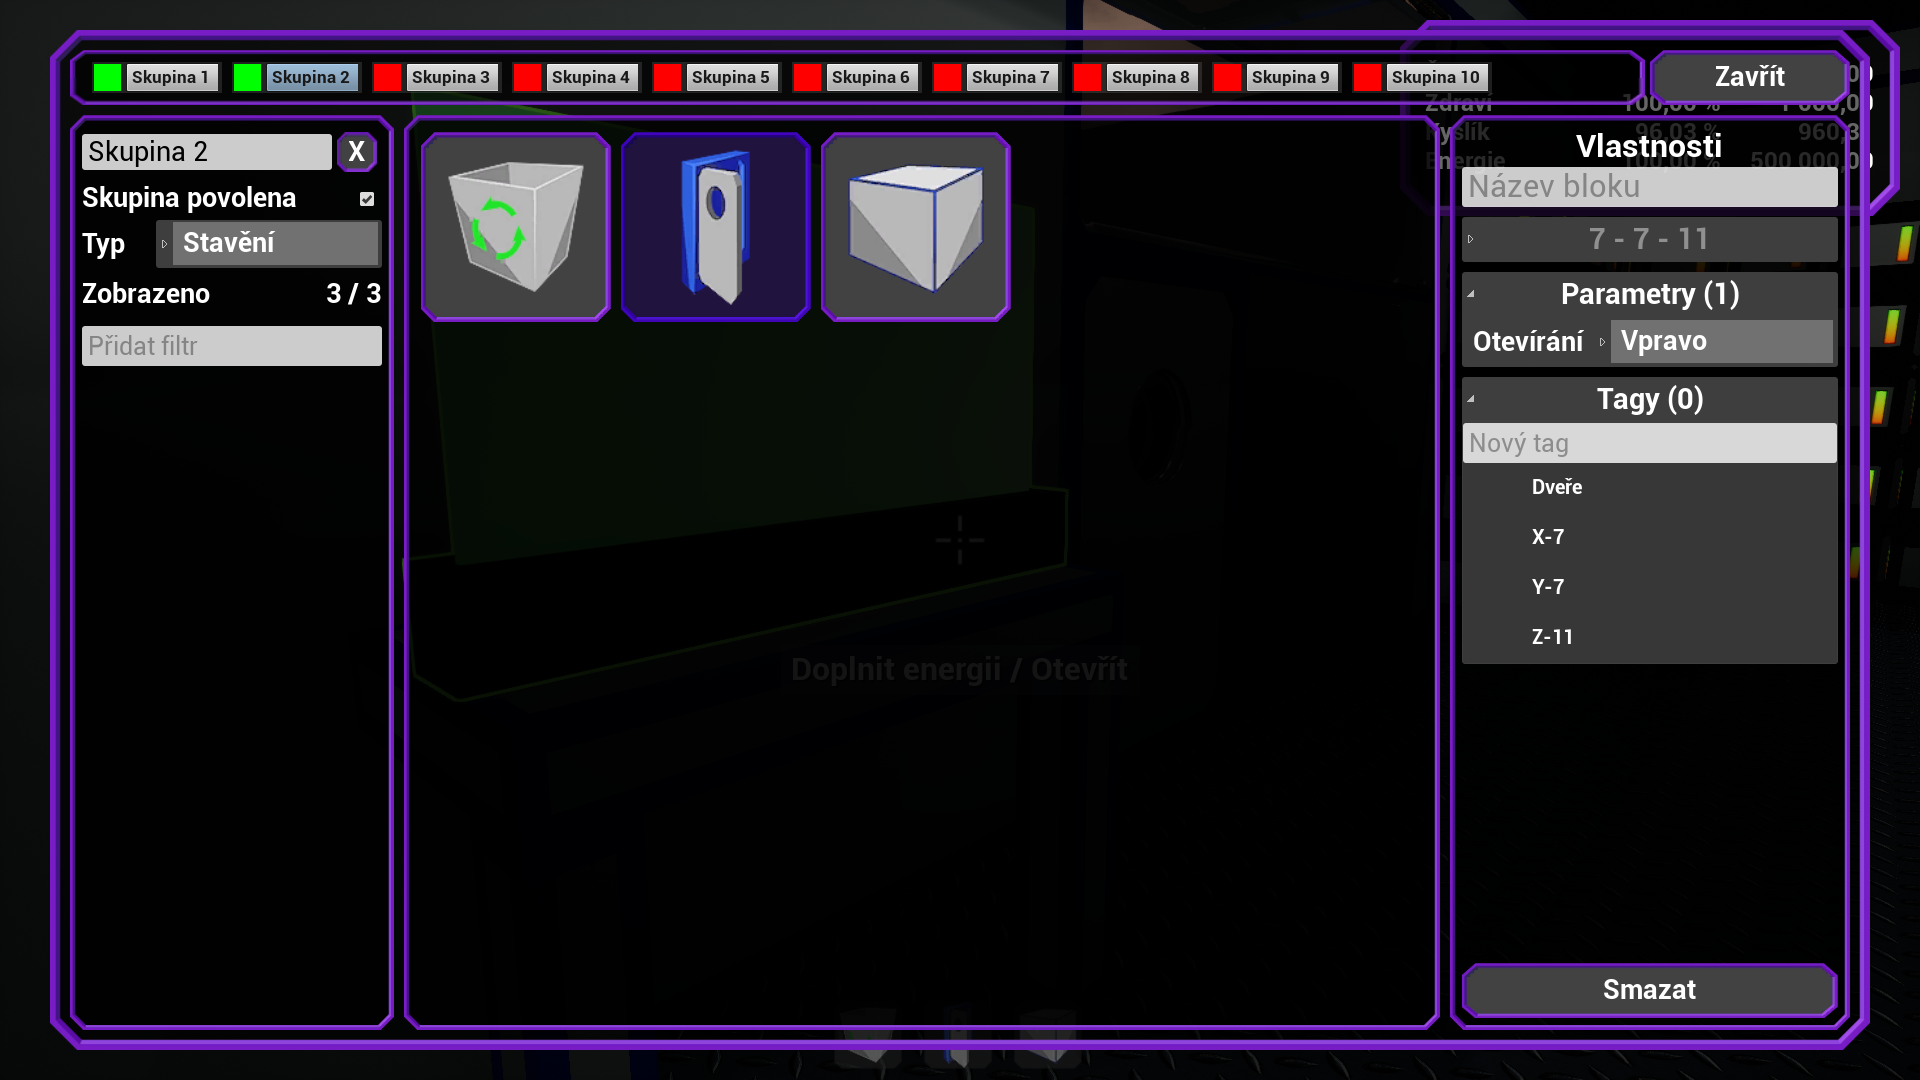
\includegraphics[ width=140mm]{../img/user/inventory/6itemWithParams}

\caption{Inventář - Nastavení}
\label{fig:user_inventory_6itemWithParams}

\end{figure}


\FloatBarrier
%!TEX root = ../prace.tex

\section{Terminál}

Pro informaci o aktuálním stavu sítě je nutné použít \textbf{Terminál}. Levým tlačítkem je možné rychle doplnit energii hráče, pravým pak otevřít ovládací obrazovku.

\begin{figure}[!h]\centering
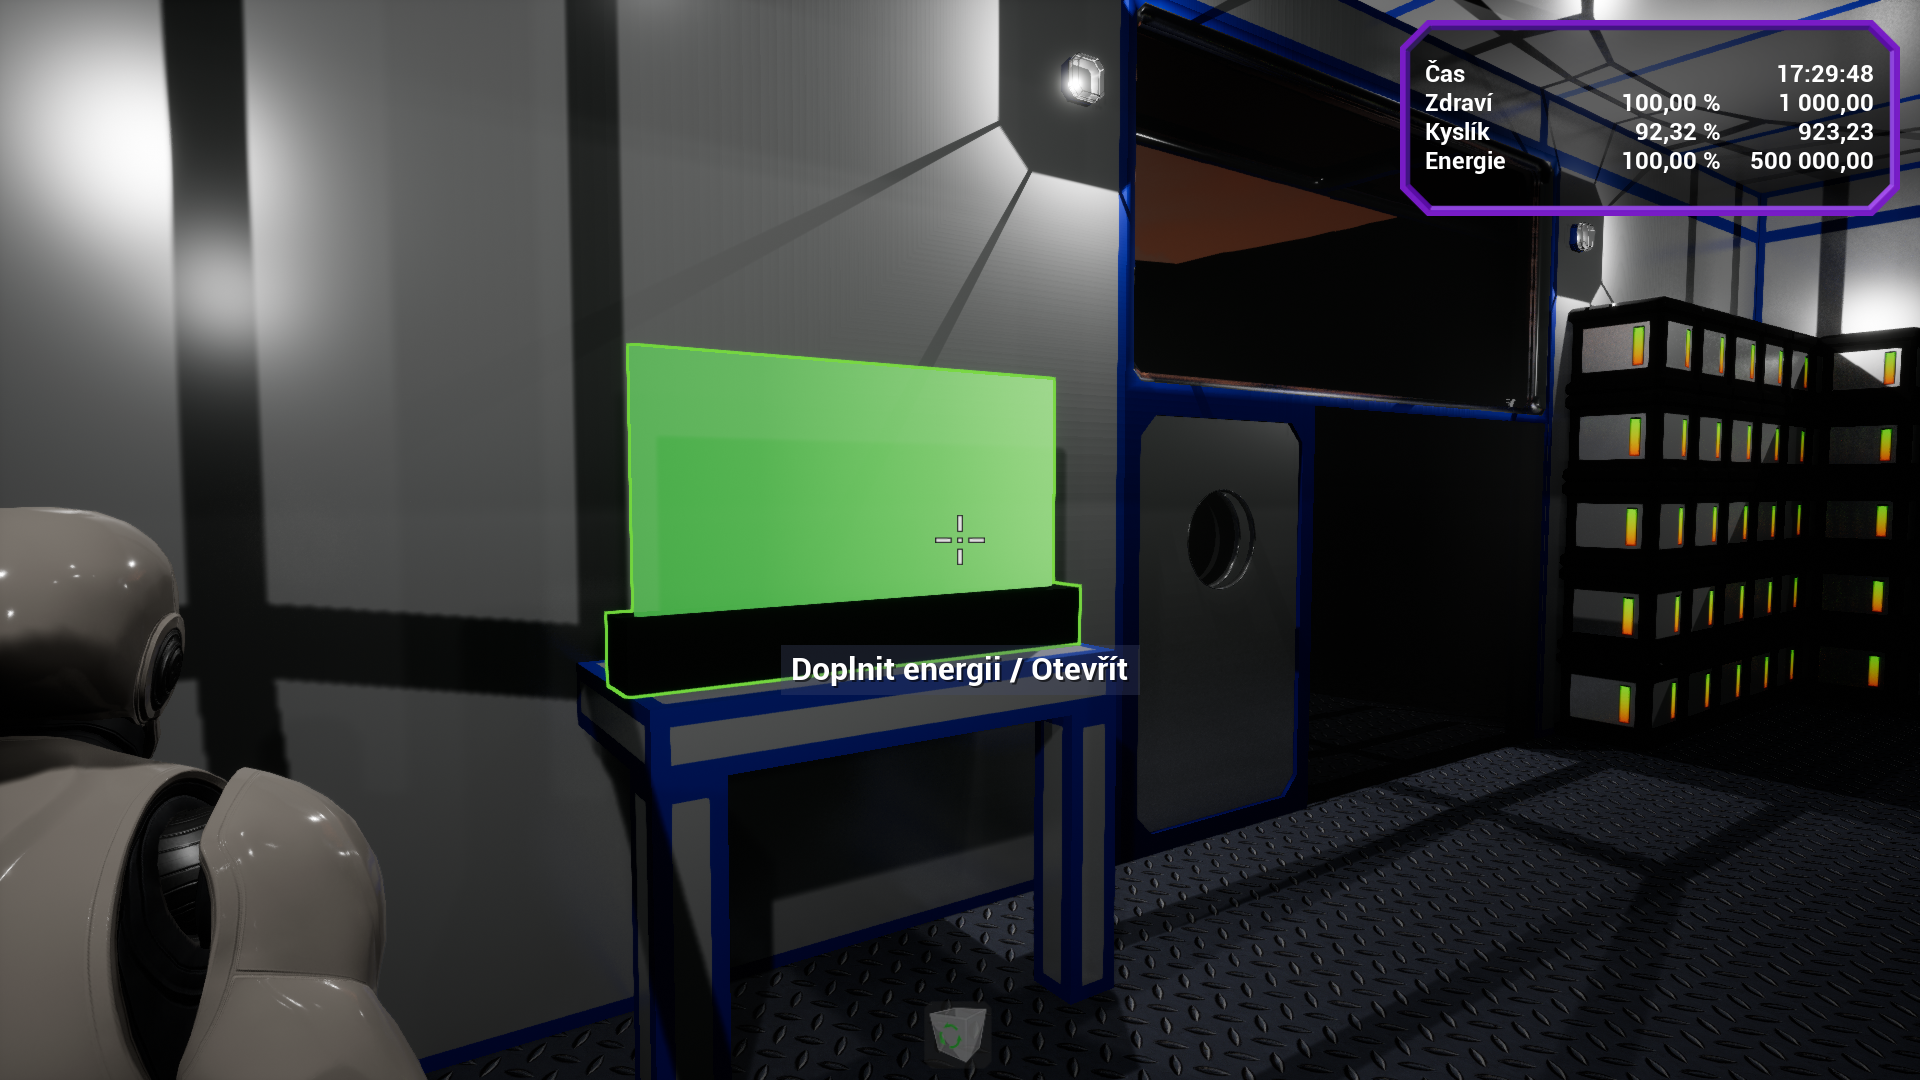
\includegraphics[ width=140mm]{../img/user/terminal/0terminalOverall}

\caption{Terminál - ve hře}
\label{fig:user_terminal_0terminalOverall}

\end{figure}

\FloatBarrier

V \textit{horní} části je vidět selektor obrazovky. Jeho rozkliknutím (více v obrázku \ref{fig:user_terminal_3terminalCtorSelector}) je možné zvolit výchozí obrazovku, nebo jeden z \textbf{Konstruktoru objektů}, které jsou v dispozici v síti.




\begin{figure}[!h]\centering
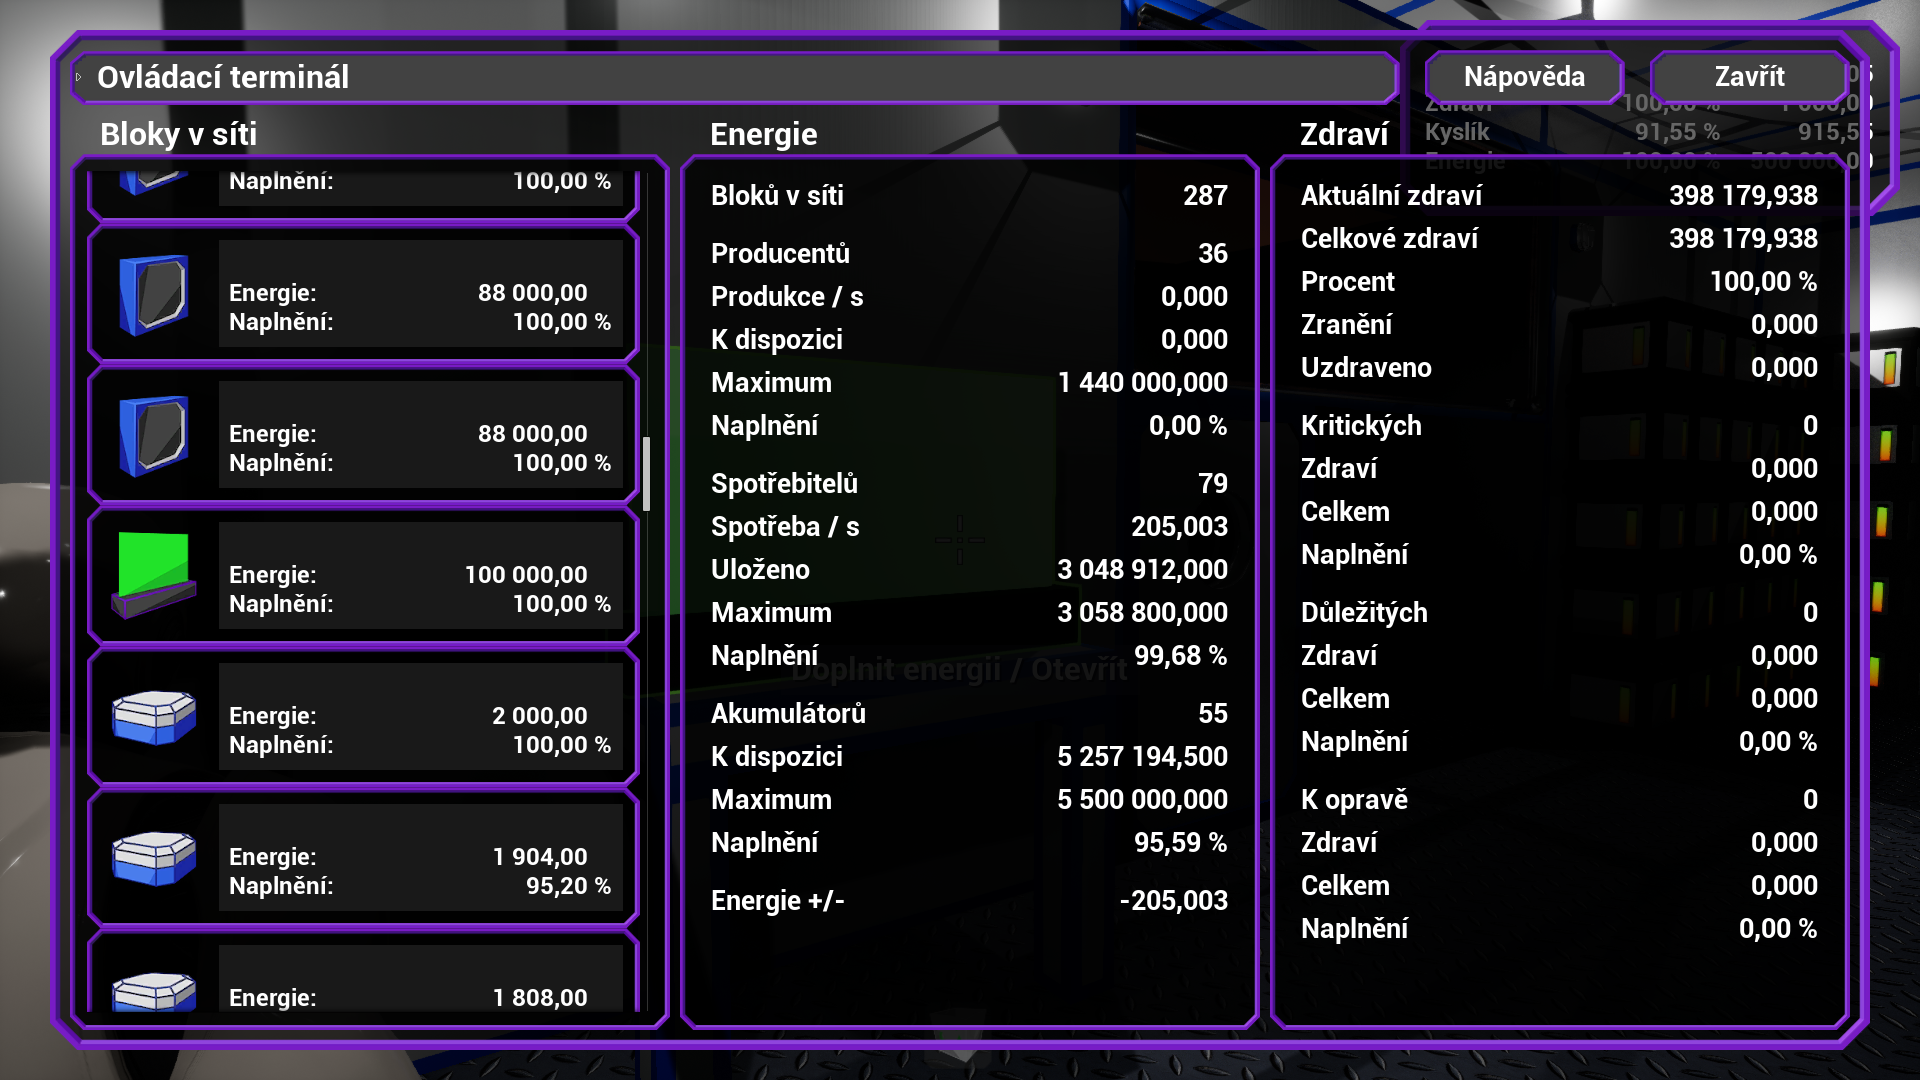
\includegraphics[ width=140mm]{../img/user/terminal/1terminalInfo}

\caption{Terminál - výchozí obrazovka}
\label{fig:user_terminal_1terminalInfo}

\end{figure}

\FloatBarrier
V \textit{levé} části je vidět seznam význačných bloků. \textit{Uprostřed} jsou vidět energetické informace o síti. \textit{Vpravo} je pak možné sledovat aktuální zdravotní stav sítě a bloků v síti.

Tlačítkem \textbf{Nápověda} je možné zobrazit informace o ovládání hry a přiřazených klávesách pro jednotlivé úkony.

\begin{figure}[!h]\centering
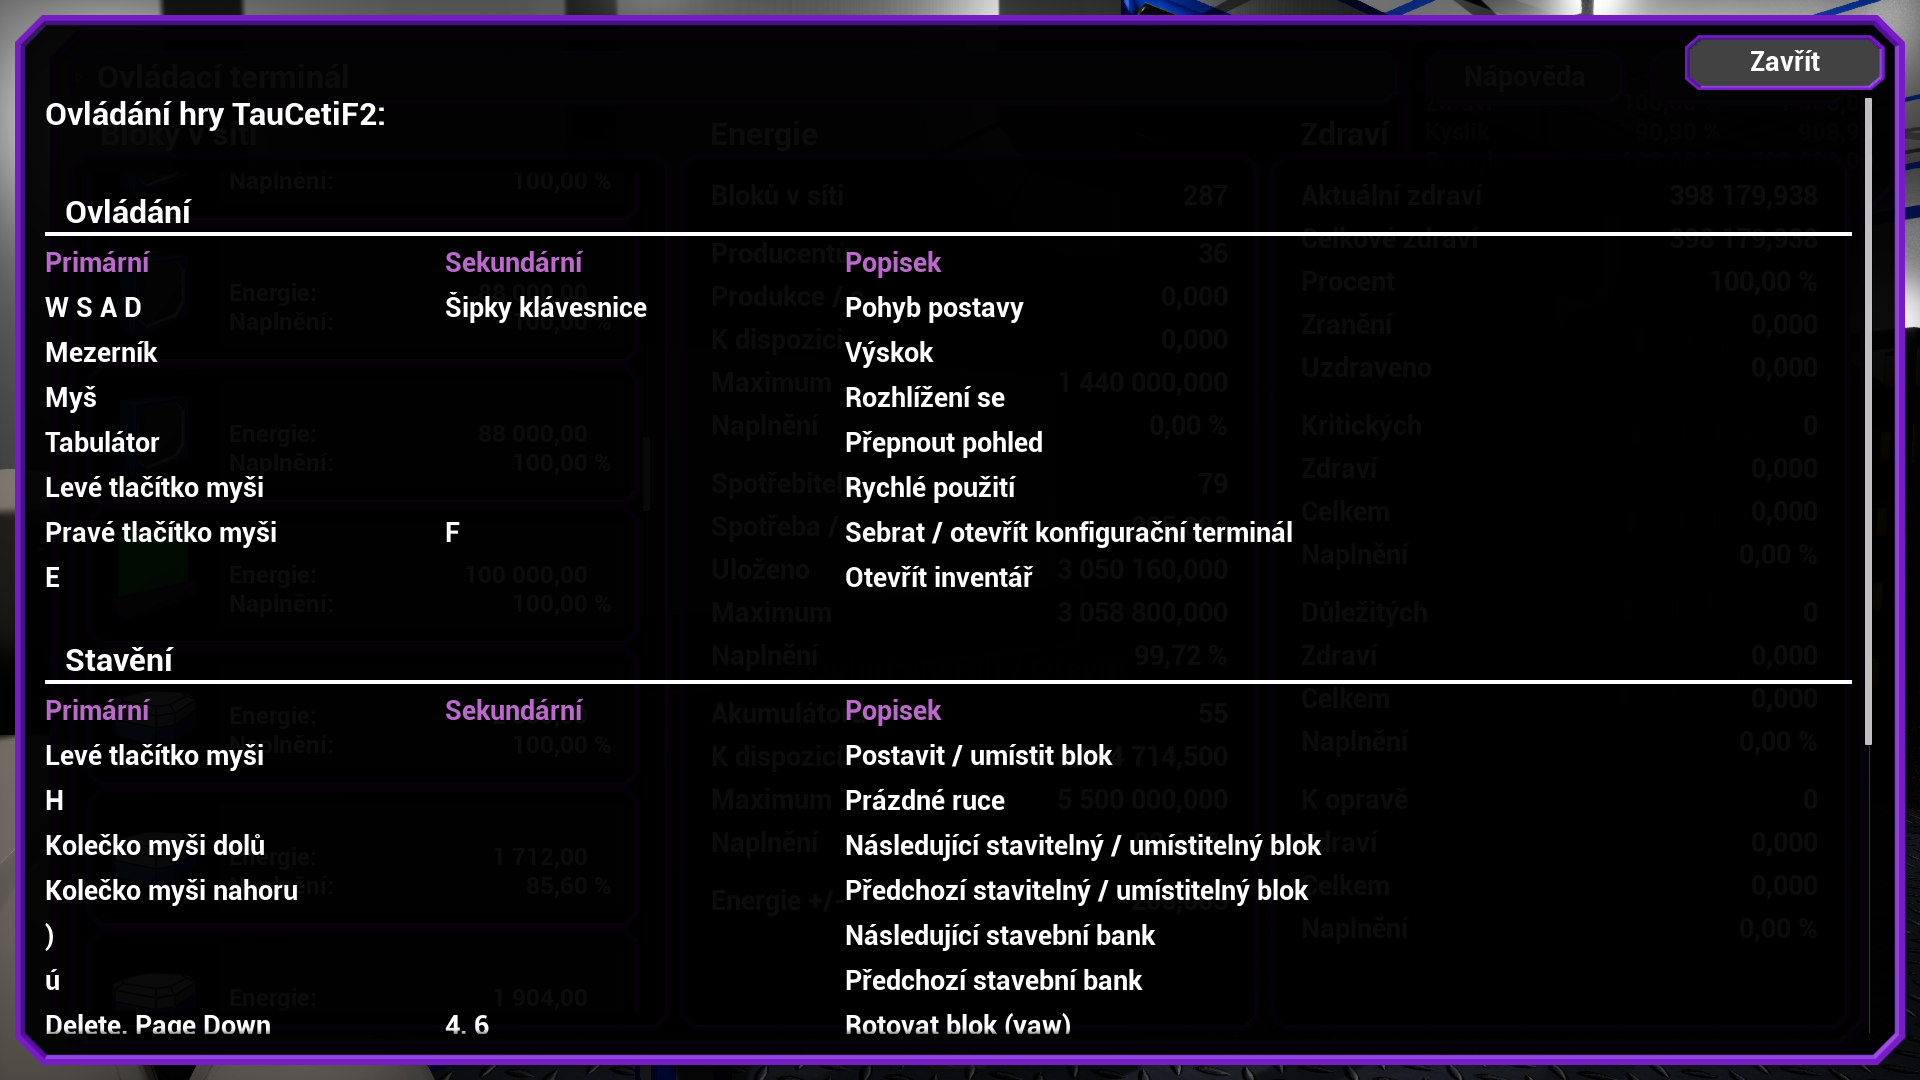
\includegraphics[ width=140mm]{../img/user/terminal/2terminalHelp}

\caption{Terminál - nápověda}
\label{fig:user_terminal_2terminalHelp}

\end{figure}

\FloatBarrier

Selektor dostupných obrazovek:

\begin{figure}[!h]\centering
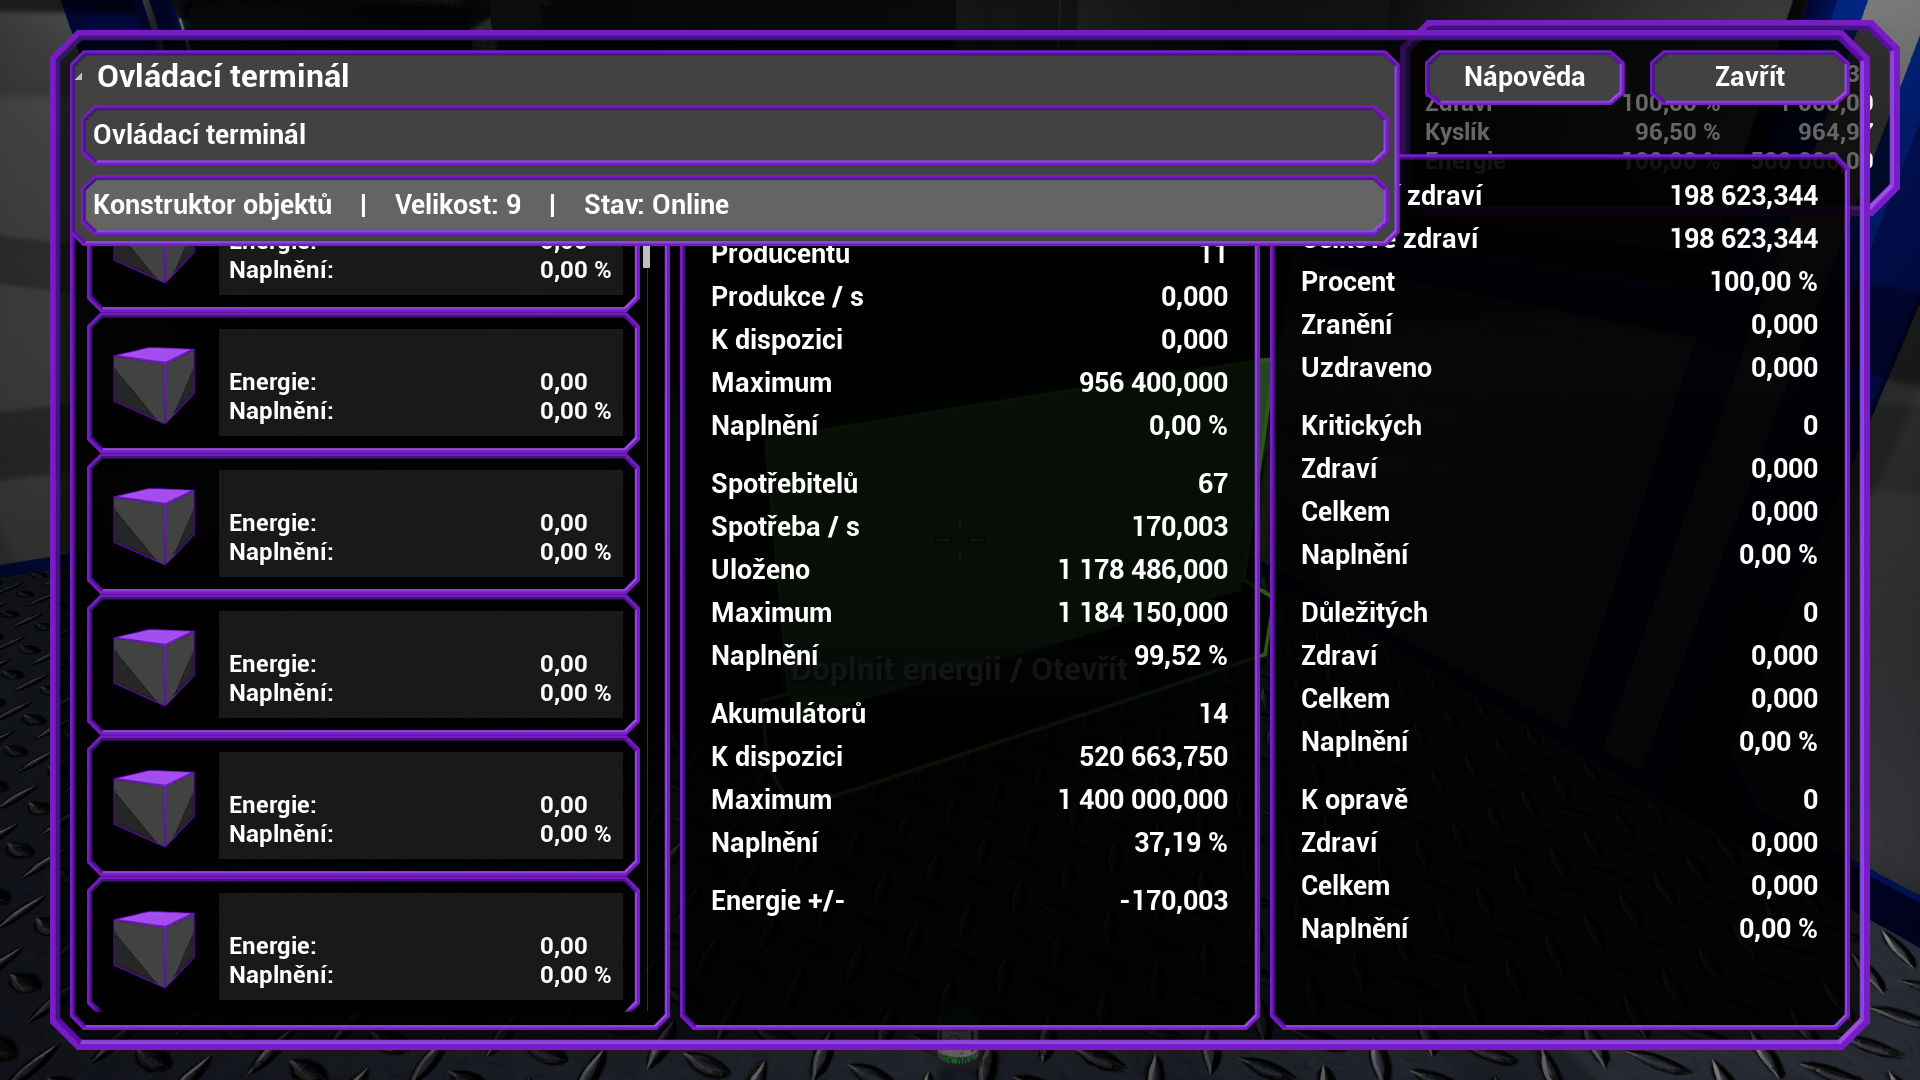
\includegraphics[ width=140mm]{../img/user/terminal/3terminalCtorSelector}

\caption{Terminál - selektor obrazovek}
\label{fig:user_terminal_3terminalCtorSelector}

\end{figure}

\FloatBarrier

Pokud vybereme \textbf{Konstruktor objektů}, vidíme seznam dostupných bloků, které můžeme zkonstruovat. Pokud to pro některé nelze (třeba z důvodu omezení velikosti - konstruktor je na daný objekt příliš malý), blok není aktivní a nelze ho zvolit.


\begin{figure}[!h]\centering
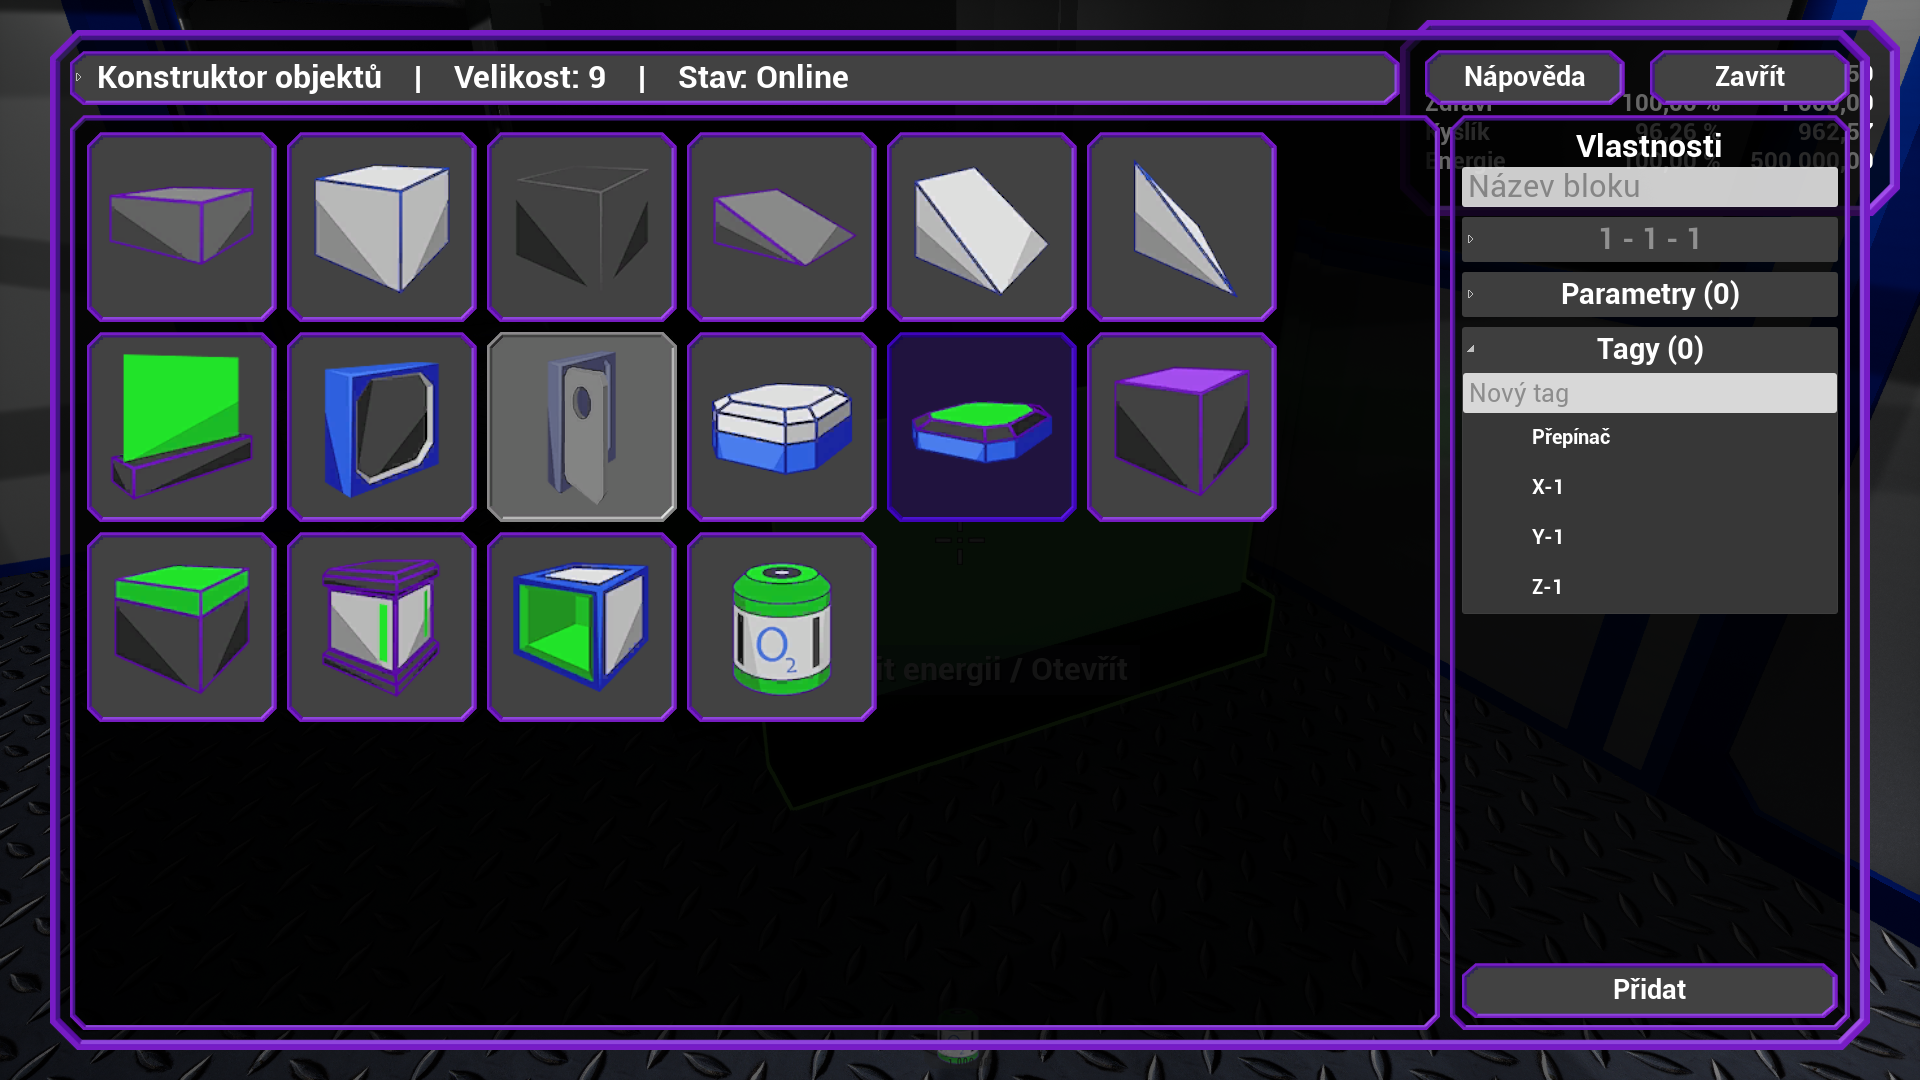
\includegraphics[ width=140mm]{../img/user/terminal/4builderSmall}

\caption{Terminál - konstruktor objektů}
\label{fig:user_terminal_4builderSmall}

\end{figure}

\FloatBarrier

V sekci \textit{Nastavení} je možné kromě tagů definovat i požadovanou velikost a to až do velikosti konstruktoru, nebo globálního omezení 20 násobku  základní kostky.

\begin{figure}[!h]\centering
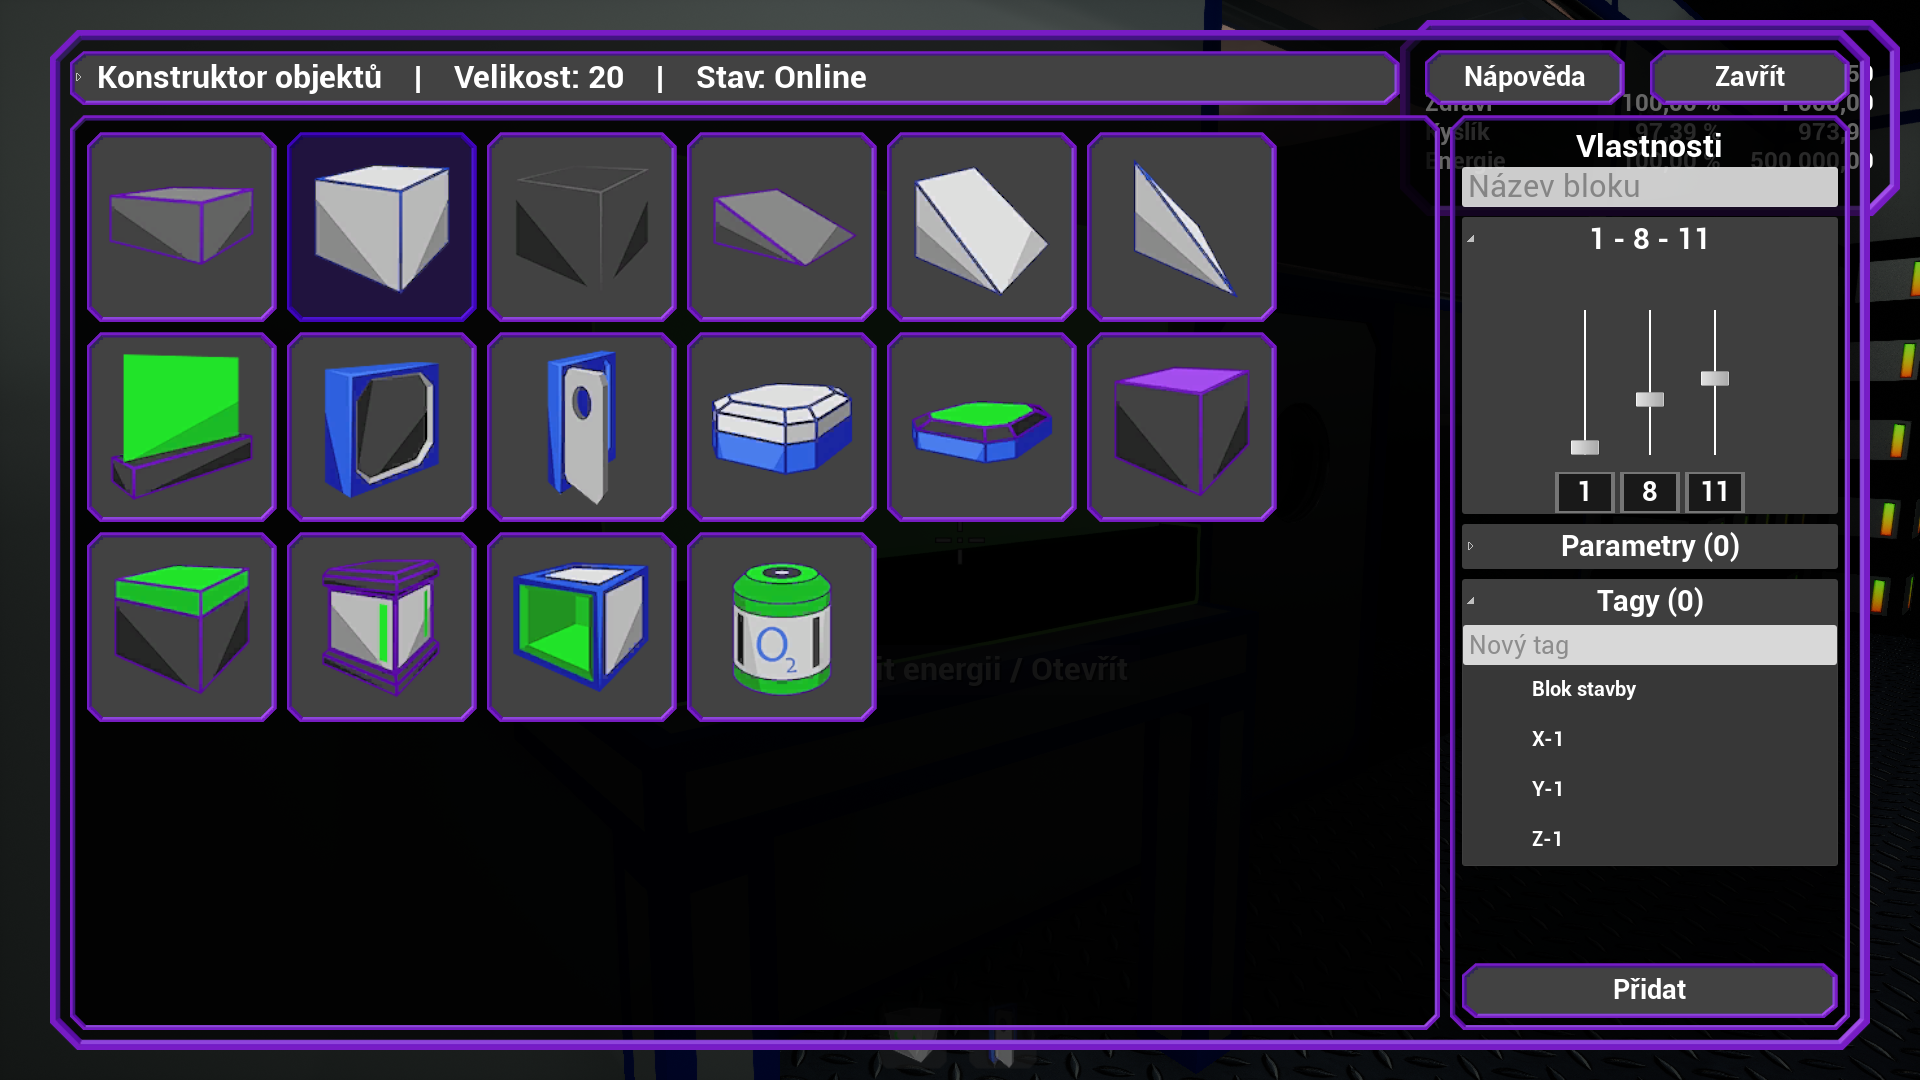
\includegraphics[ width=140mm]{../img/user/terminal/5builderSize}

\caption{Terminál - Nastavení velikosti}
\label{fig:user_terminal_5builderSize}

\end{figure}

\FloatBarrier

Některé bloky, třeba \textbf{Dveře} požadují dodatečné parametry, které ovlivňují jejich výsledné chování. V našem případě to je smysl otevírání dveří při čelním pohledu. Na obrázku je vidět stav po rozkliknutí.

\begin{figure}[!h]\centering
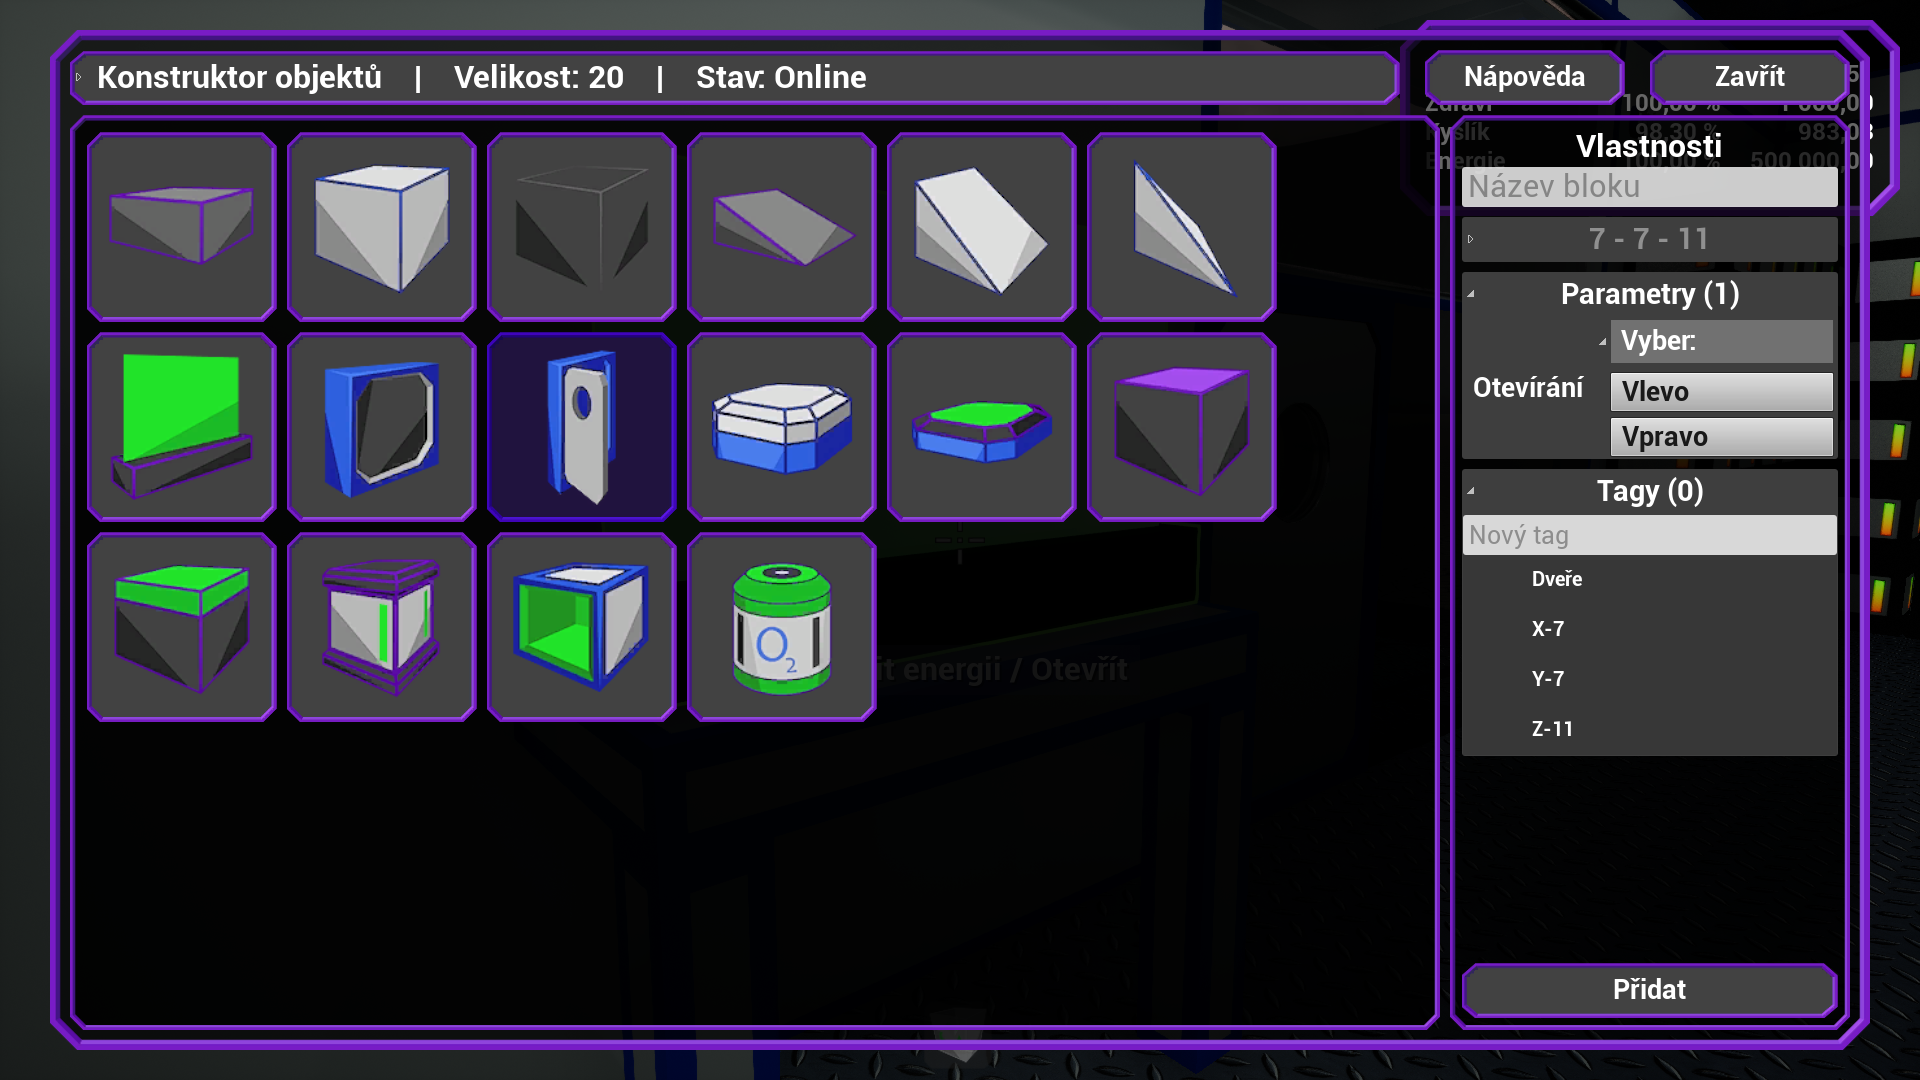
\includegraphics[ width=140mm]{../img/user/terminal/6builderParams}

\caption{Terminál - Nastavení parametrů}
\label{fig:user_terminal_6builderParams}

\end{figure}

\FloatBarrier
%!TEX root = ../../prace.tex

\section{Stavební akce}

\textbf{Destruktor} umožňuje mazat bloky. Po jeho výběru je vidět červený outline vybraného bloku.

\begin{figure}[!ht]\centering
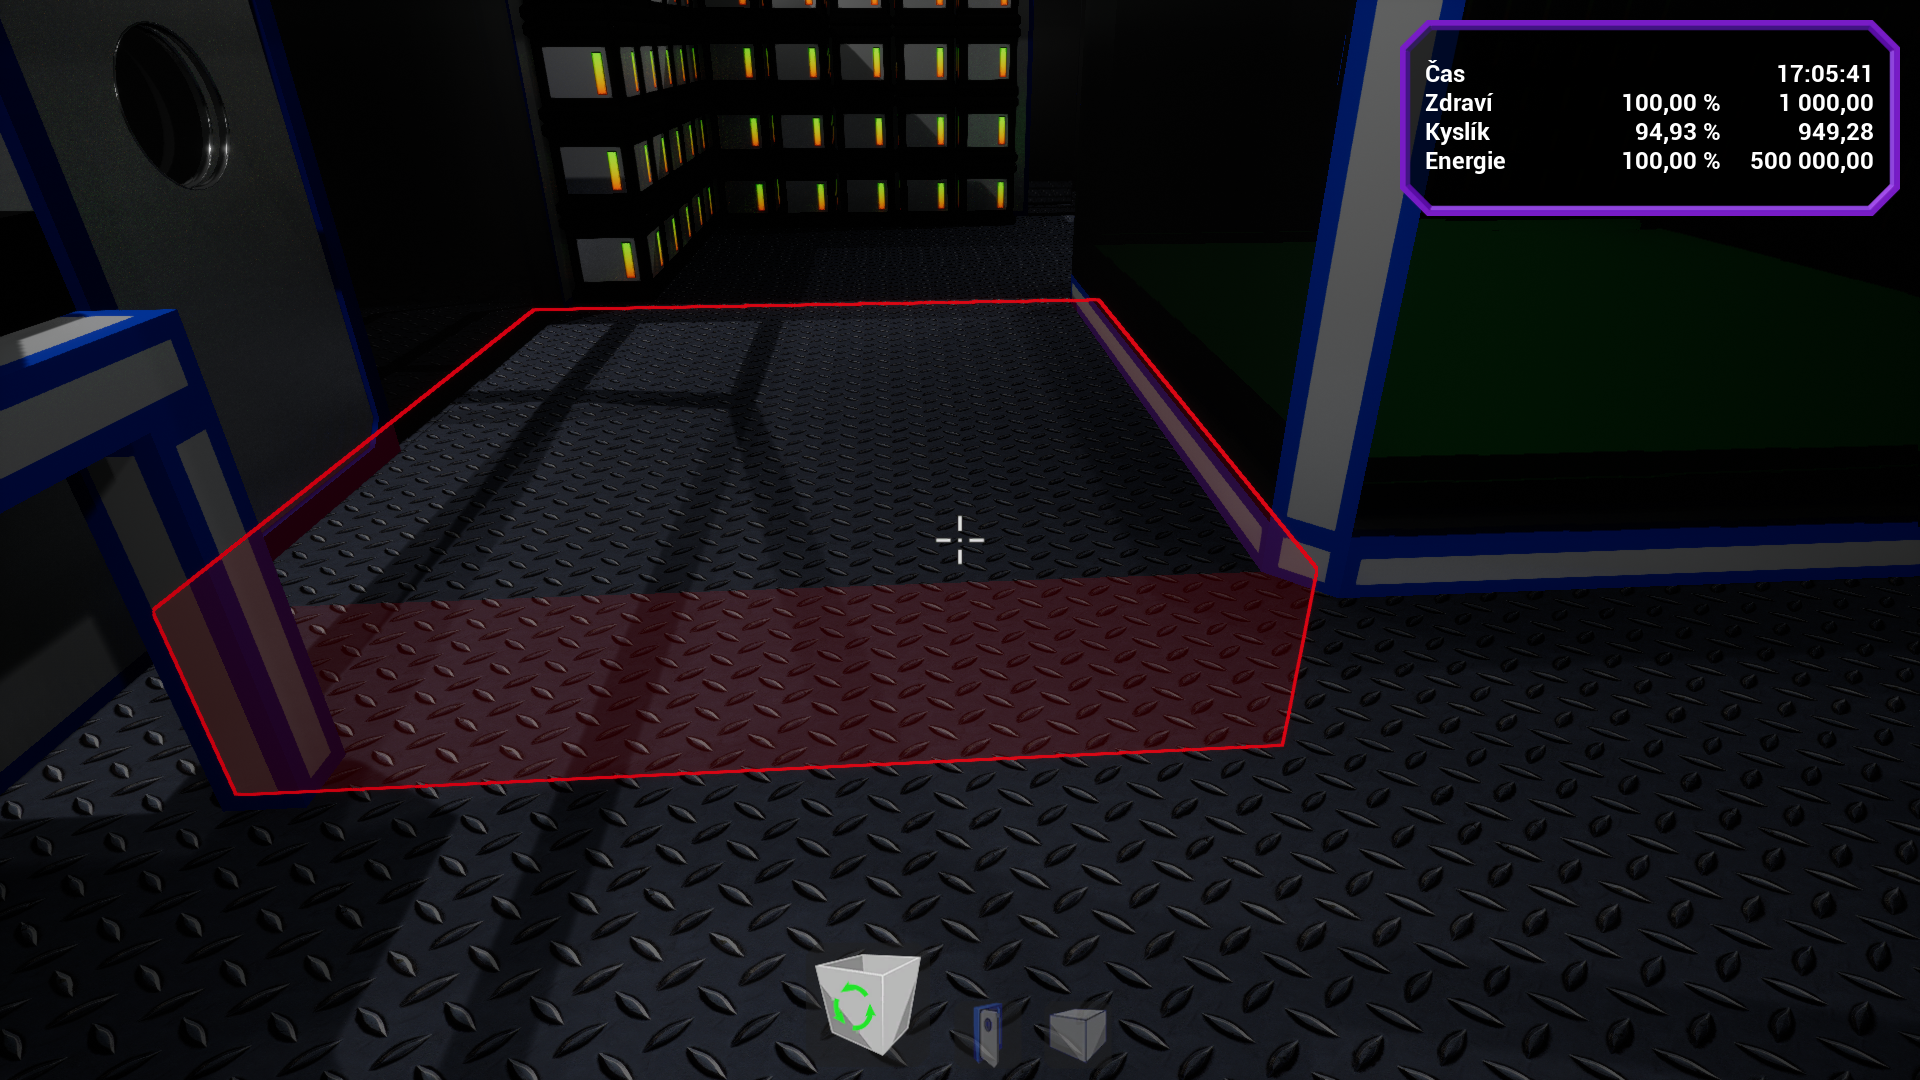
\includegraphics[ width=140mm]{../img/user/buildActions/delete}

\caption{Stavění -- smazat}
\label{fig:user_buildActions_delete}

\end{figure}

\FloatBarrier

Pokud vybereme umístění nového bloku, vidíme žlutě hranice sousedního bloku, ke kterému blok přistavujeme. Stavěný / umisťovaný blok musí mít dostatečné místo pro svoje umístění. Dále je potřeba mít s~sebou dostatečně velkou zásobu energie (dle energetické náročnosti bloku).

\begin{figure}[!ht]\centering
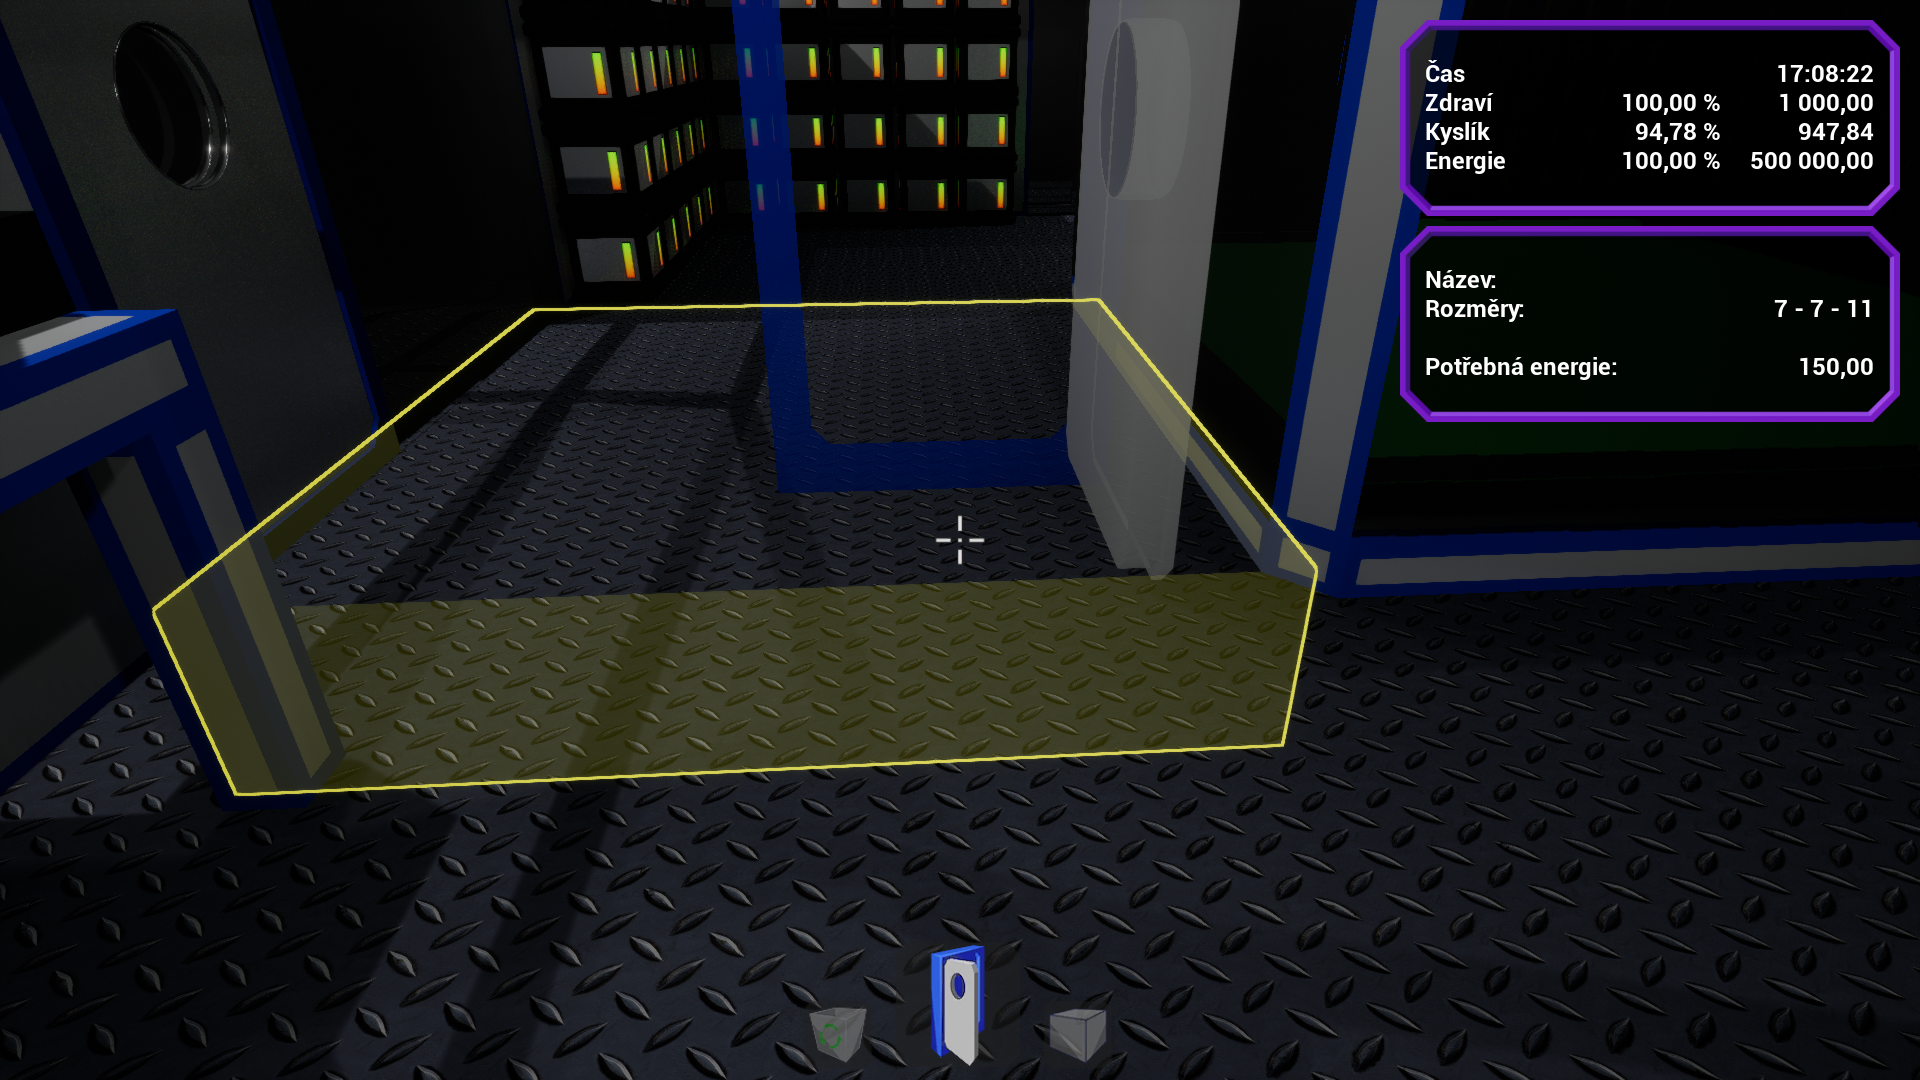
\includegraphics[ width=140mm]{../img/user/buildActions/place}

\caption{Stavění -- umístit}
\label{fig:user_buildActions_place}

\end{figure}

\FloatBarrier

Blok je též možný rotovat (Klávesy v~sekci Insert .. Page Down, případně jejich ekvivalenty 7,8,9,4,5,6).

\begin{figure}[!ht]\centering
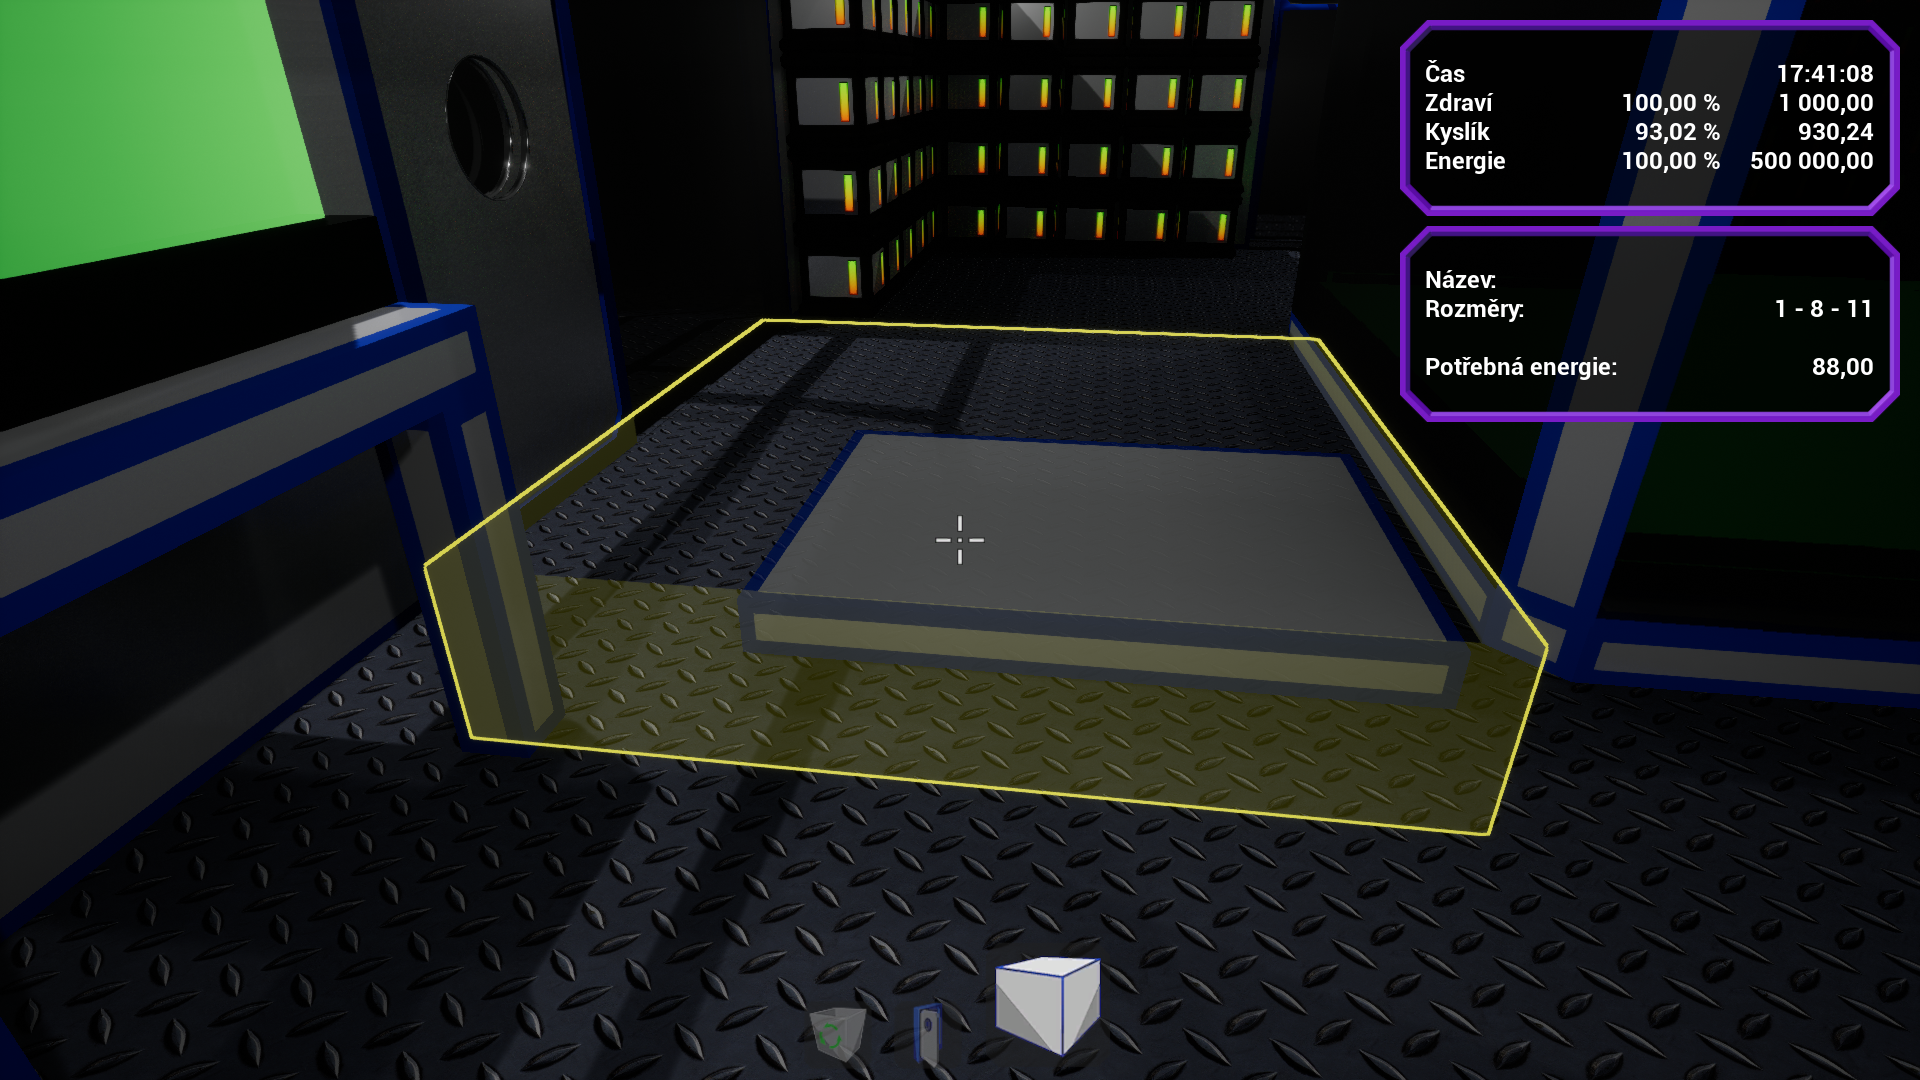
\includegraphics[ width=140mm]{../img/user/buildActions/place_Rotate}

\caption{Stavění -- rotace}
\label{fig:user_buildActions_place_Rotate}

\end{figure}

\FloatBarrier

Pokud bylo umístění v~pořádku, blok již není nadále průhledný a~hráči ubyla energie. Pokud je zapnut kreativní mód, energie samozřejmě neubývá.

\begin{figure}[!ht]\centering
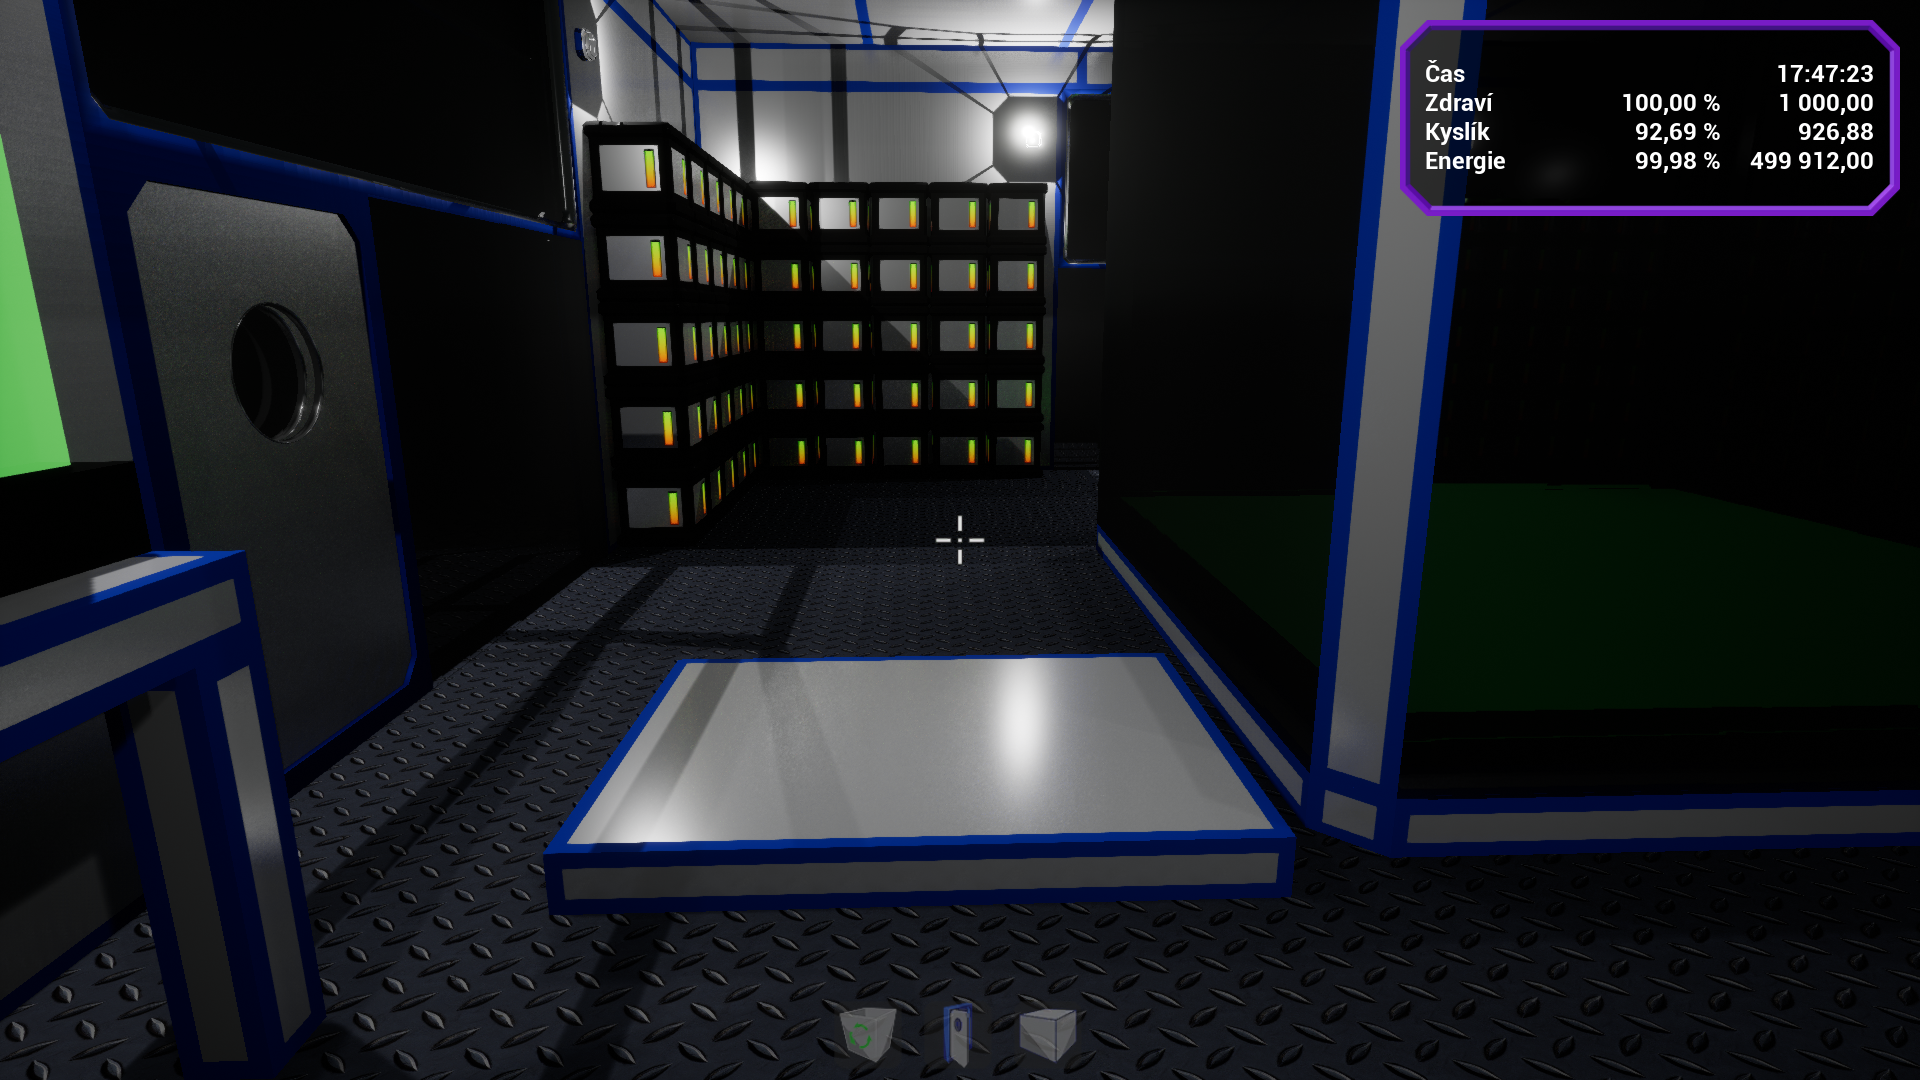
\includegraphics[ width=140mm]{../img/user/buildActions/placeAfter}

\caption{Stavění -- po umístění}
\label{fig:user_buildActions_placeAfter}

\end{figure}


\FloatBarrier
%!TEX root = ../../prace.tex

\section{Umístitelné předměty}

Blok \textbf{Kyslíková bomba} je možné umístit do světa a pak si ho opět vzít do inventáře. Díky tomu je možné tyto bloky dále používat třeba pro plnění v \textbf{Plničce kyslíkových bomb}.
Blok je možné buď rovnou použít (levé tlačítko myši).
Tento blok zároveň rovnou ukazuje, kolik objemu je využito.

\begin{figure}[!ht]\centering
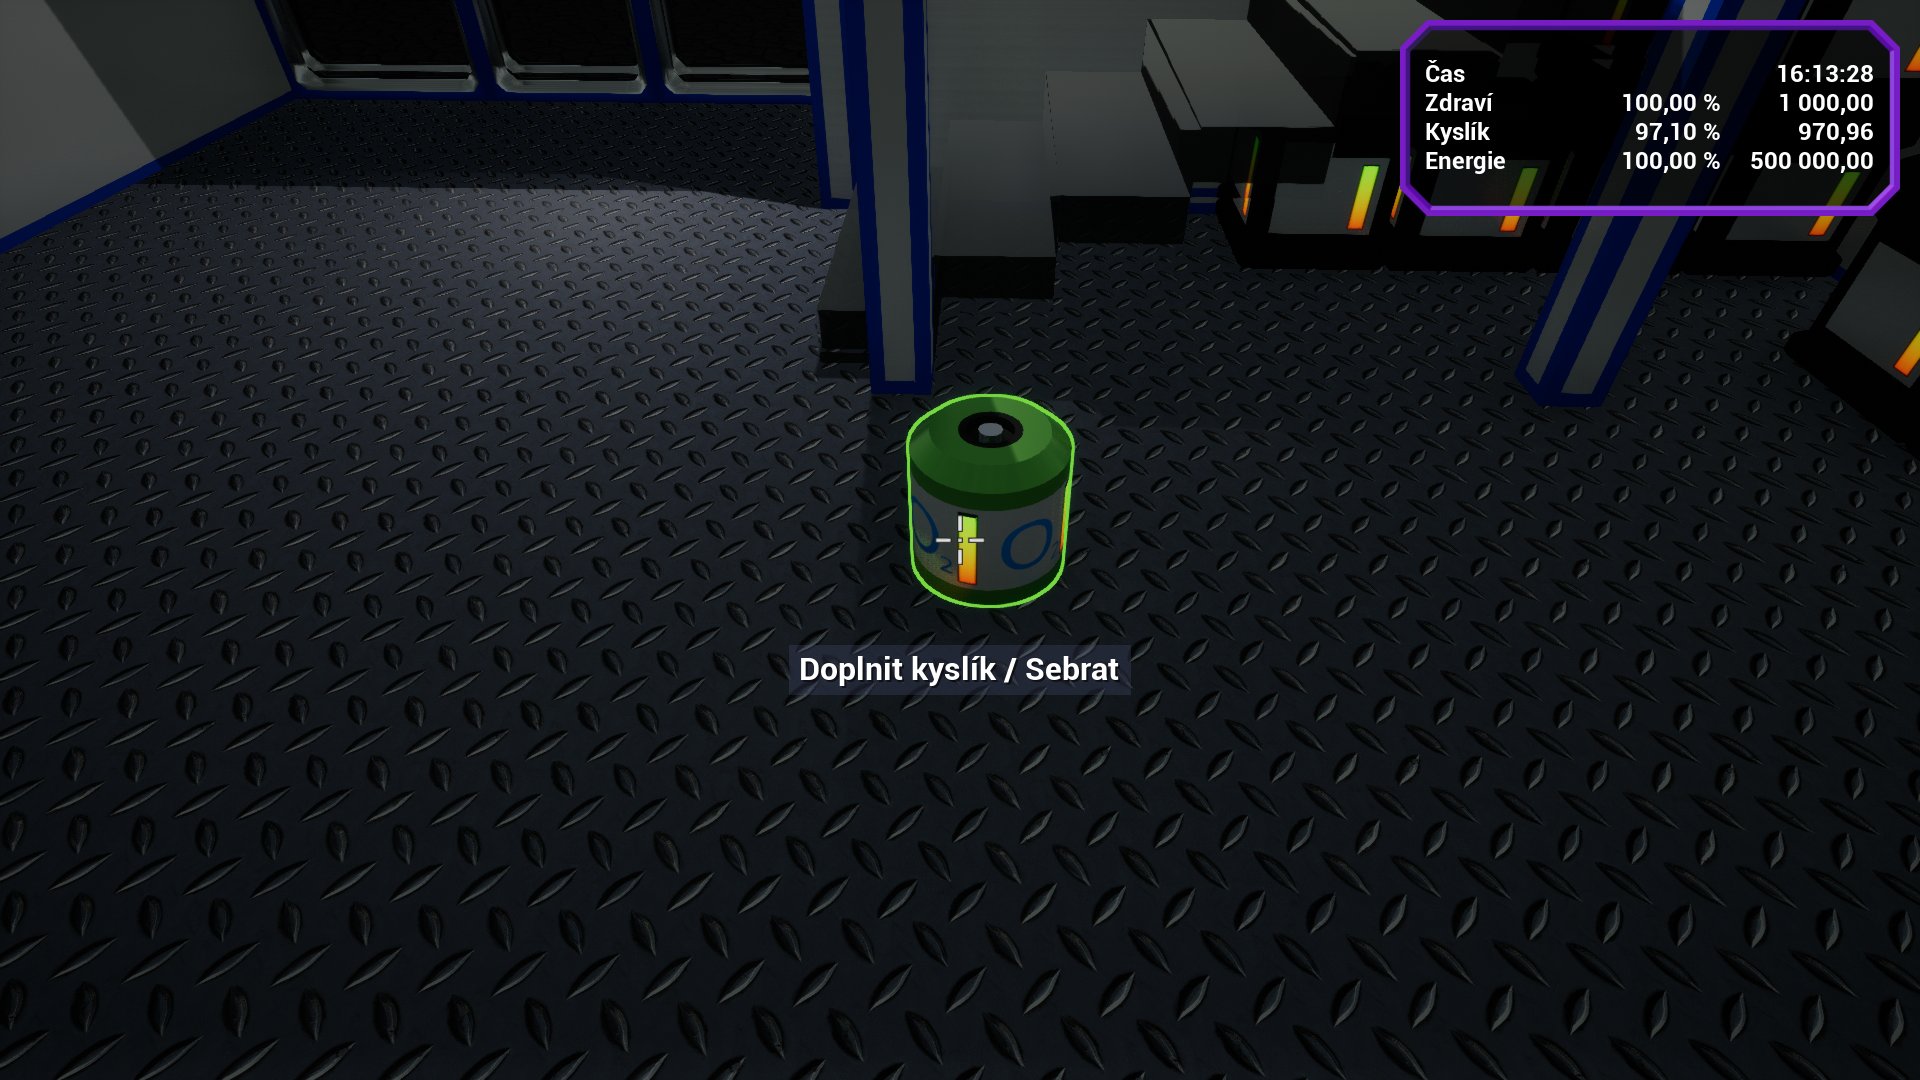
\includegraphics[ width=140mm]{../../img/user/tank/0tankFull}

\caption{Umístitelné předměty - plná kyslíková bomba}
\label{fig:user_tank_0tankFull}

\end{figure}

\FloatBarrier

Na dalším obrázku vidíme již částečně použitou kyslíkovou bombu. Pokud ji pravým tlačítkem myši sebereme a otevřeme si inventář a správnou skupinu (\textbf{Typ: Inventář} v nastavení skupiny), uvidíme tento blok v seznamu.

Požité tagy se při přidání do světa a opětovném sebrání zachovávají.

\begin{figure}[!ht]\centering
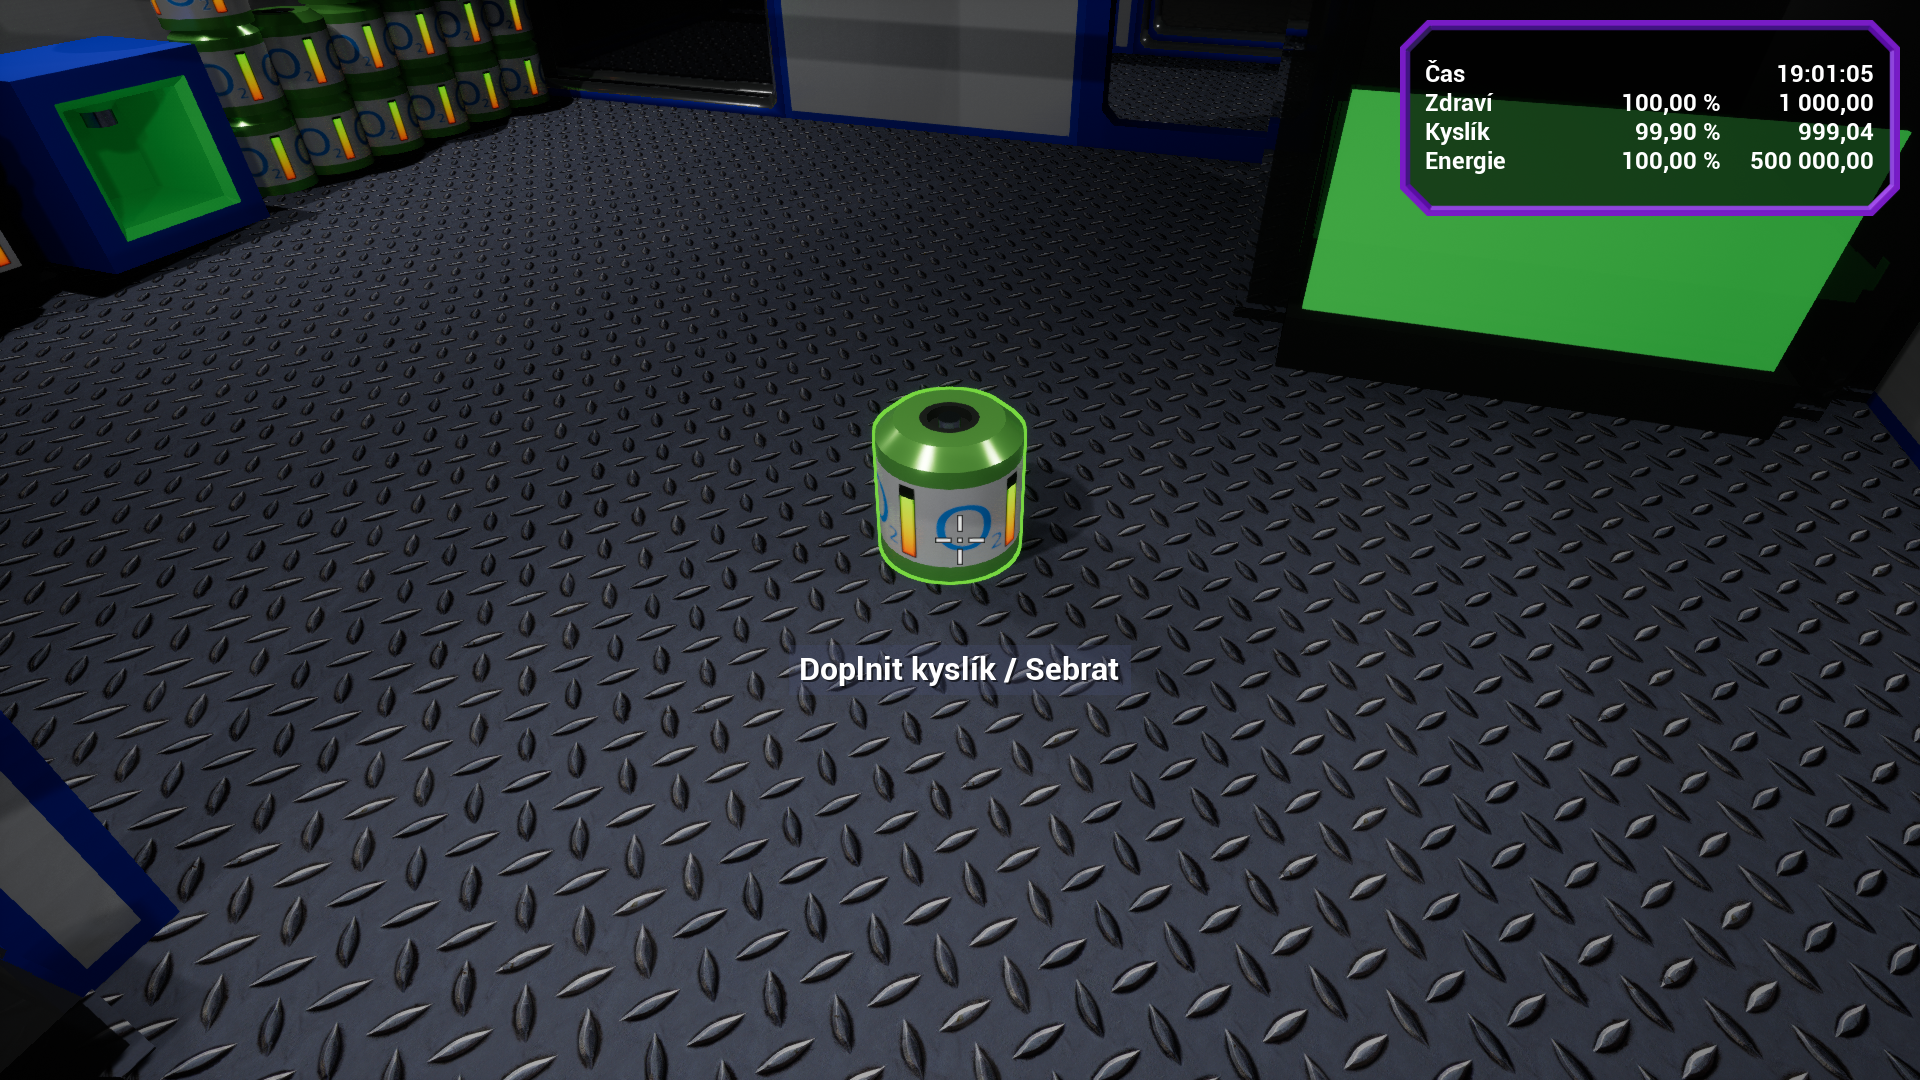
\includegraphics[ width=140mm]{../../img/user/tank/1tankAfterUse}

\caption{Umístitelné předměty - použitá bomba}
\label{fig:user_tank_1tankAfterUse}

\end{figure}

\FloatBarrier

Zároveň v inventáři můžeme vidět přesnou hodnotu naplnění bloku.

\begin{figure}[!ht]\centering
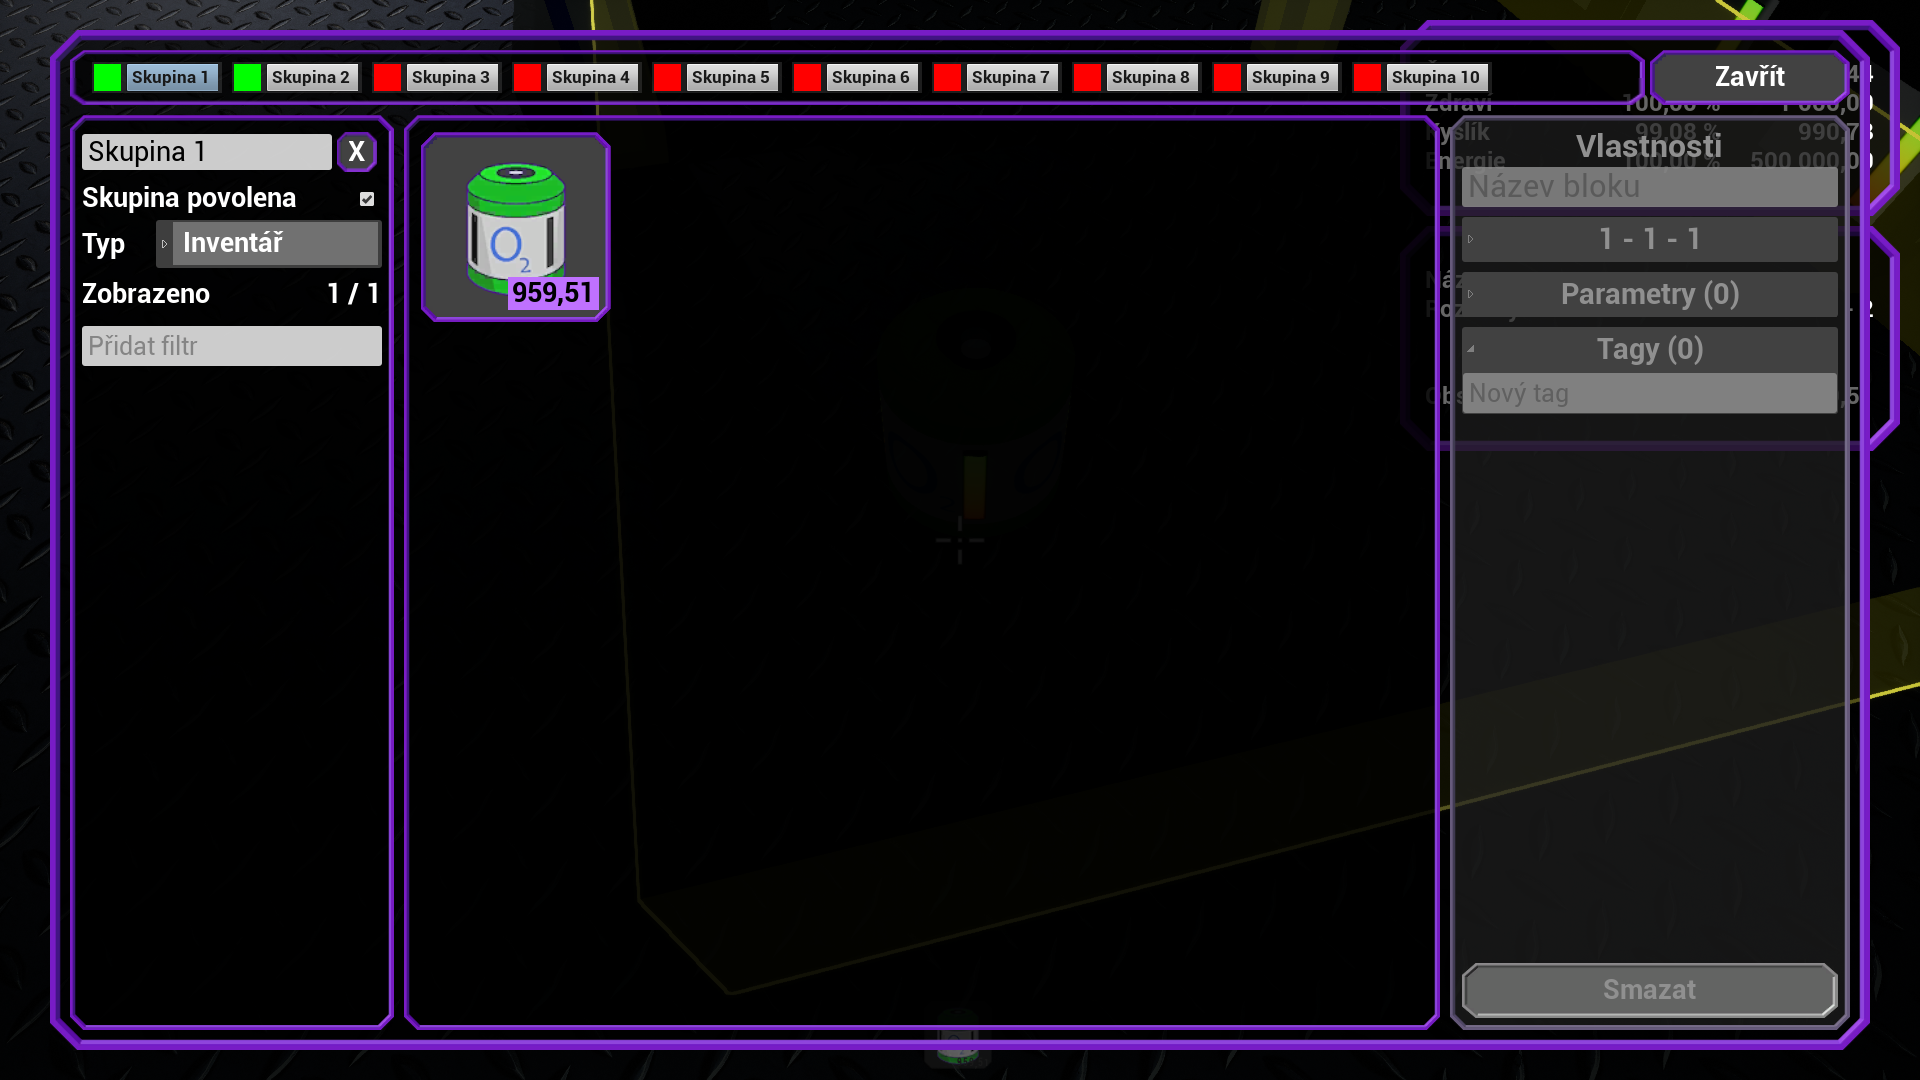
\includegraphics[ width=140mm]{../../img/user/tank/2tankInventory}

\caption{Umístitelné předměty - inventář}
\label{fig:user_tank_2tankInventory}

\end{figure}



\FloatBarrier
%!TEX root = ../../prace.tex

\section{Plnička kyslíkových bomb}

Kyslíkové bomby je potřeba opětovně naplnit, pokud byl jejich obsah spotřebován. Stejně jako u~Kyslíkové bomby, levým tlačítkem myši je možné rovnou doplnit zásoby kyslíku hráče. Pravým se pak otevře ovládací obrazovka.

\begin{figure}[!ht]\centering
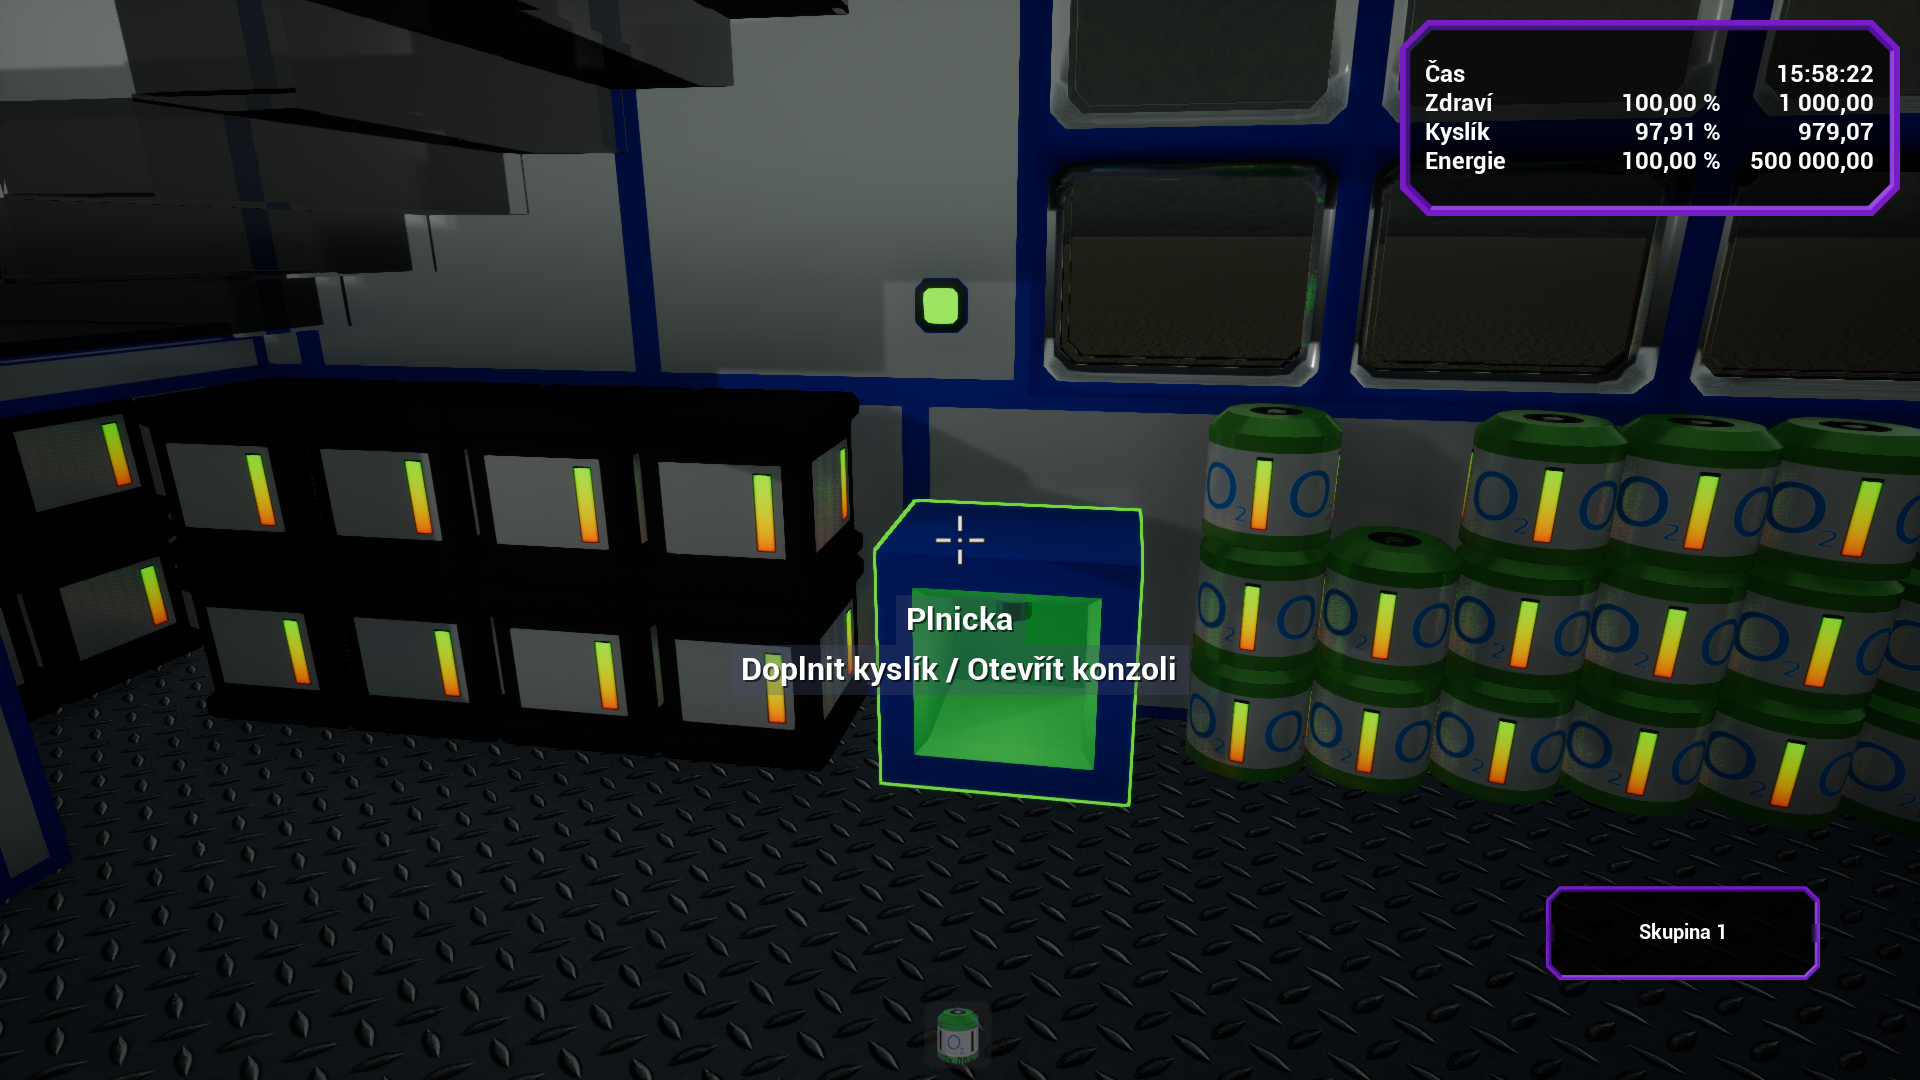
\includegraphics[ width=140mm]{../img/user/filler/0use}

\caption{Plnička kyslíkové bomby -- náhled}
\label{fig:user_filler_0use}

\end{figure}

\FloatBarrier

Ta má v~levé části přiřazený ovladač, případně je možné nejvýše jeden ovladač ze seznamu ovladačů přiřadit. Pokud je přiřazen ovladač, zapnutí bloku se řídí jeho nastavením. V~pravé části je možné regulovat spotřebovávanou energii.

Uprostřed je možné vybrat bomby, které jsou v~inventáři hráče, k~naplnění.

\begin{figure}[!ht]\centering
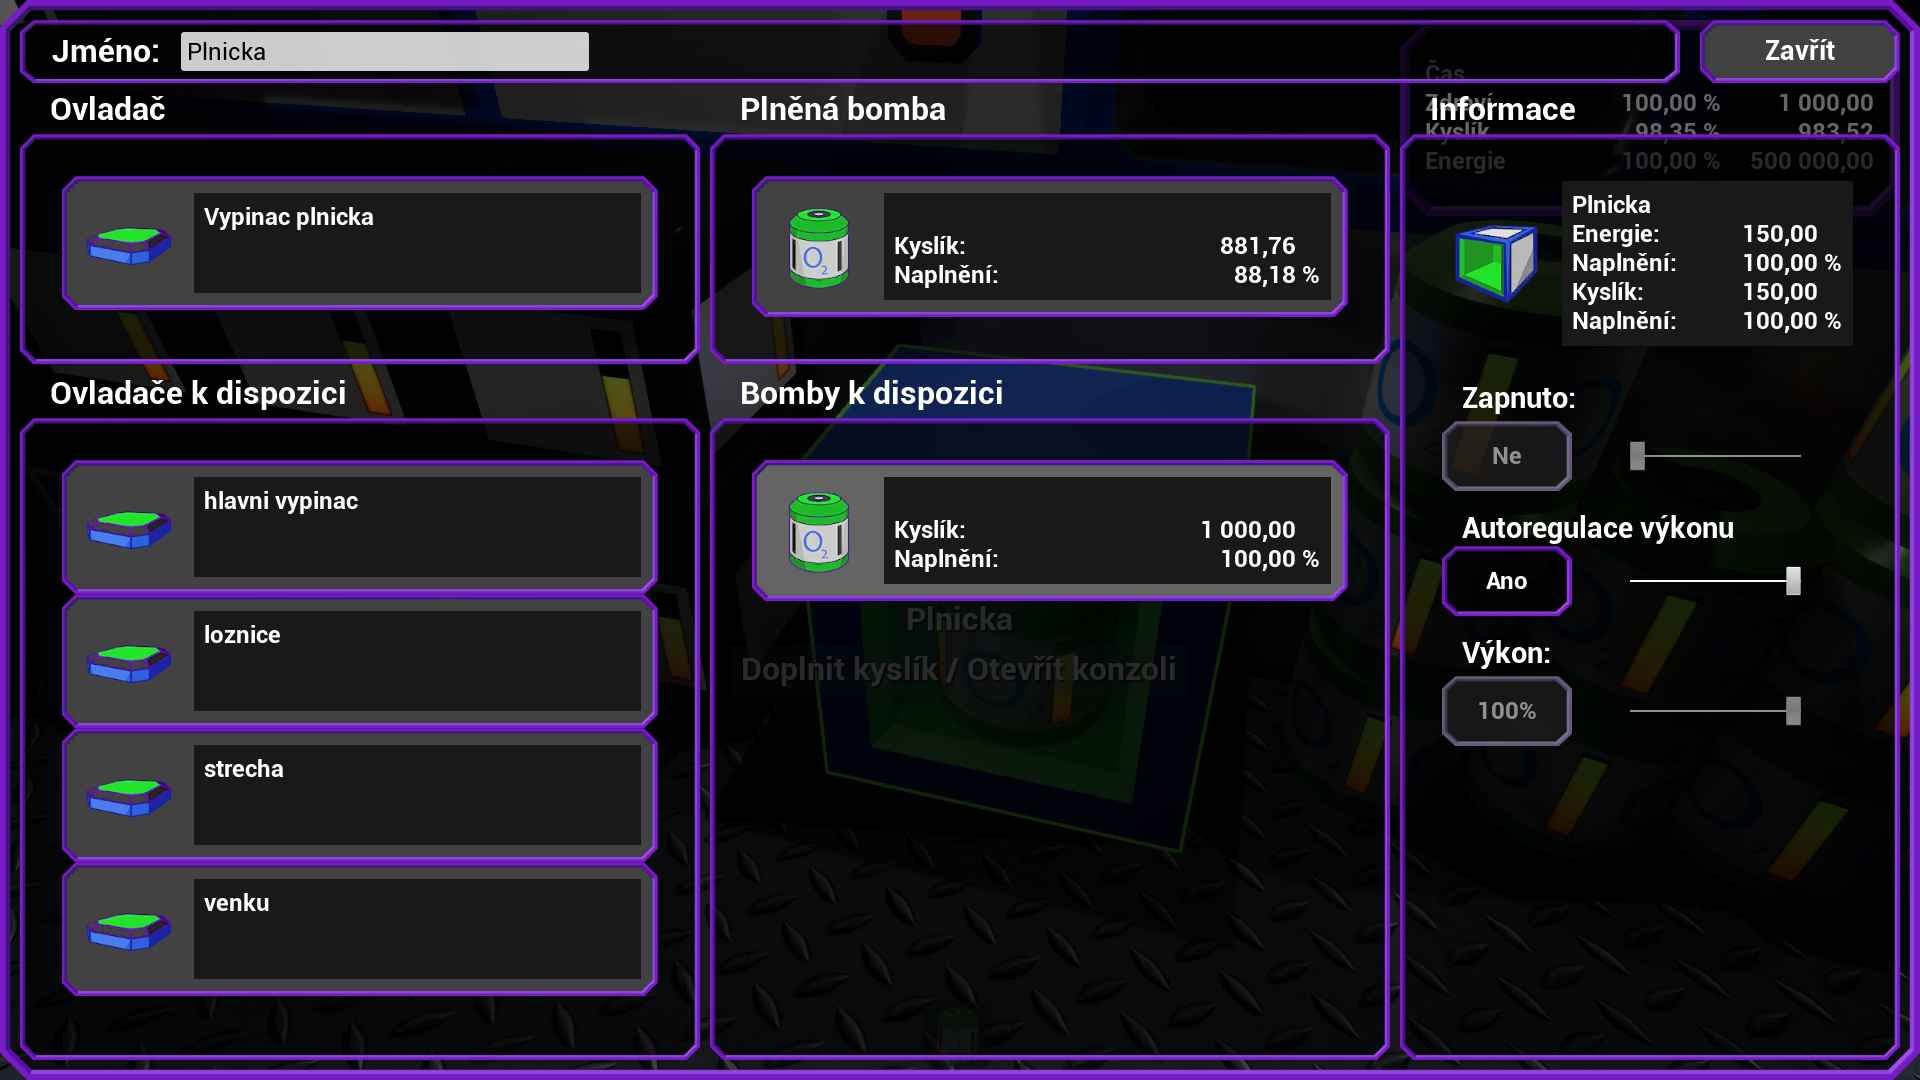
\includegraphics[ width=140mm]{../img/user/filler/1fill}

\caption{Plnička kyslíkové bomby -- ovládací obrazovka}
\label{fig:user_filler_1fill}

\end{figure}

\FloatBarrier

Pokud je plnička zapnuta, generuje kyslík a~ze své zásoby plní přiřazenou kyslíkovou bombu.

\begin{figure}[!ht]\centering
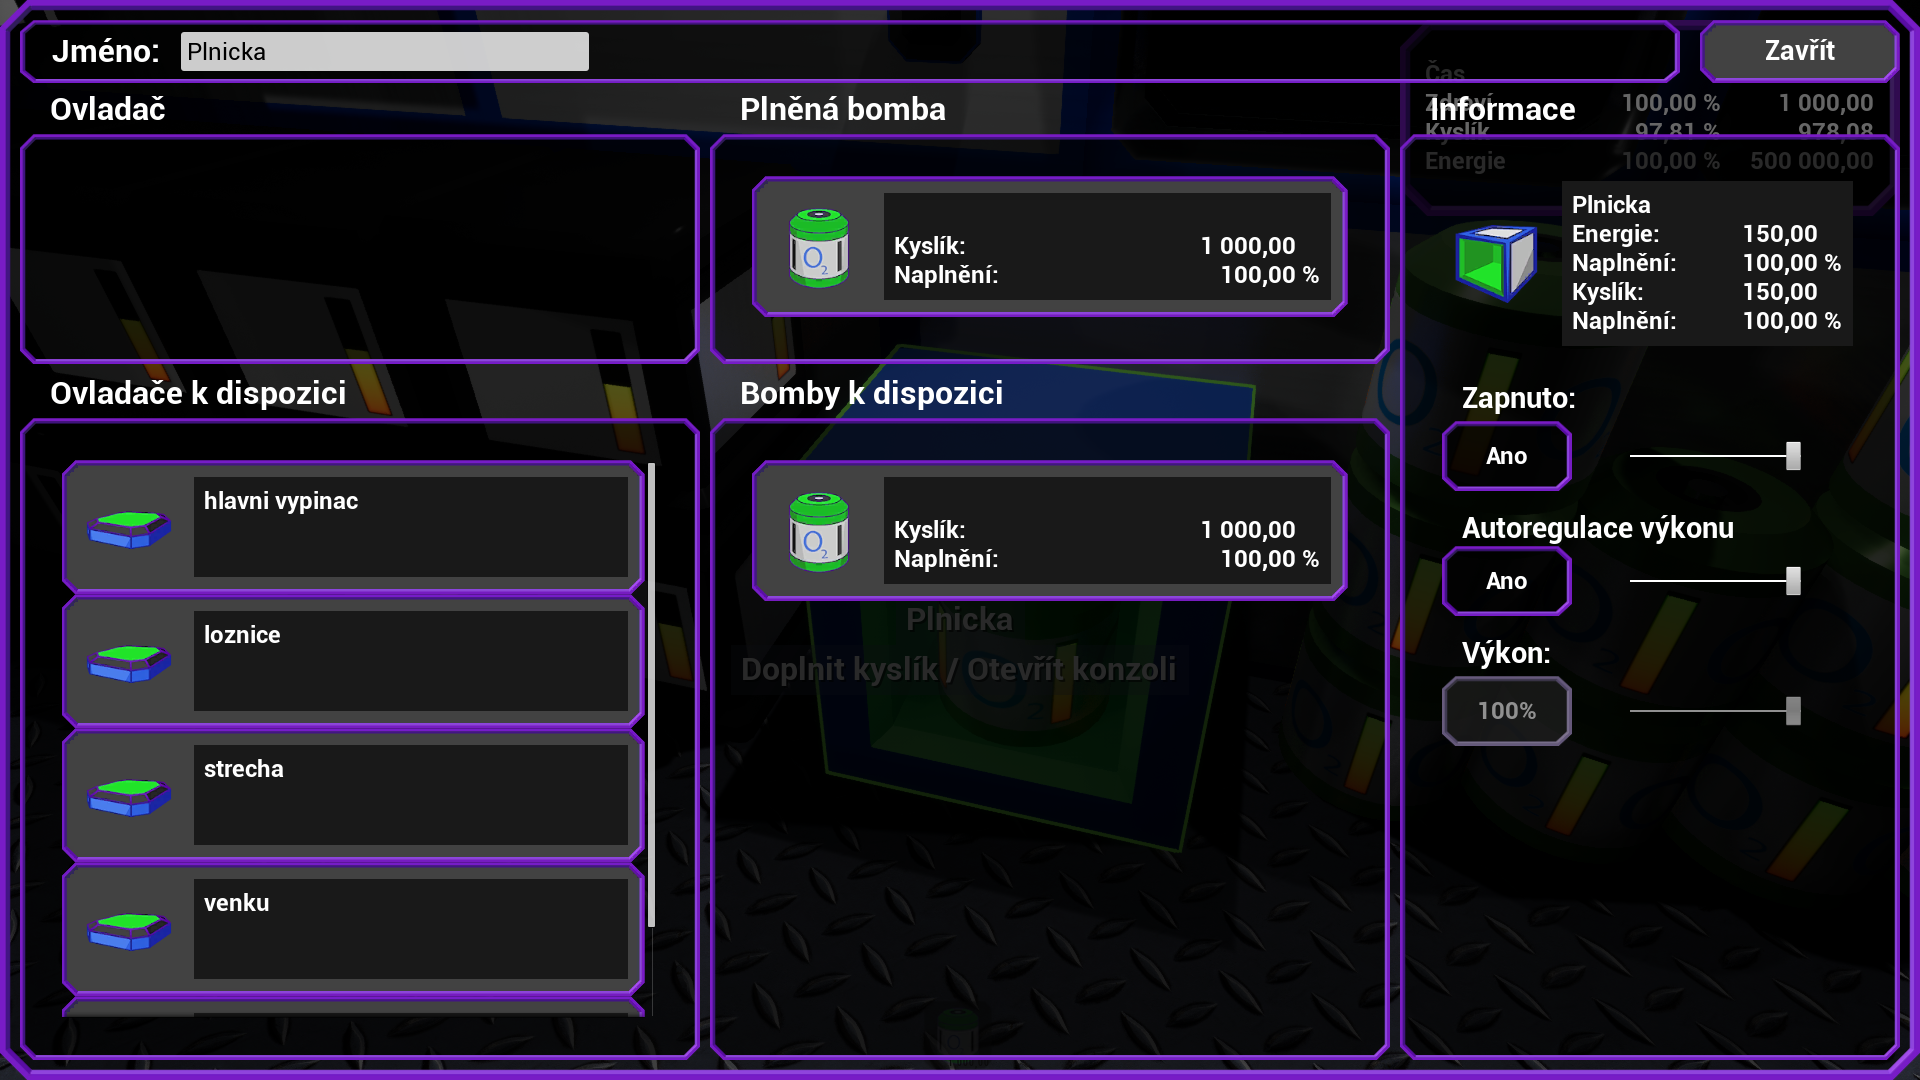
\includegraphics[ width=140mm]{../img/user/filler/2filled}

\caption{Plnička kyslíkové bomby -- naplněno}
\label{fig:user_filler_2filled}

\end{figure}



\FloatBarrier
%!TEX root = ../prace.tex

\section{Přepínač}

Přepínač slouží jako ovládání pro světla a plničku

\begin{figure}[!h]\centering
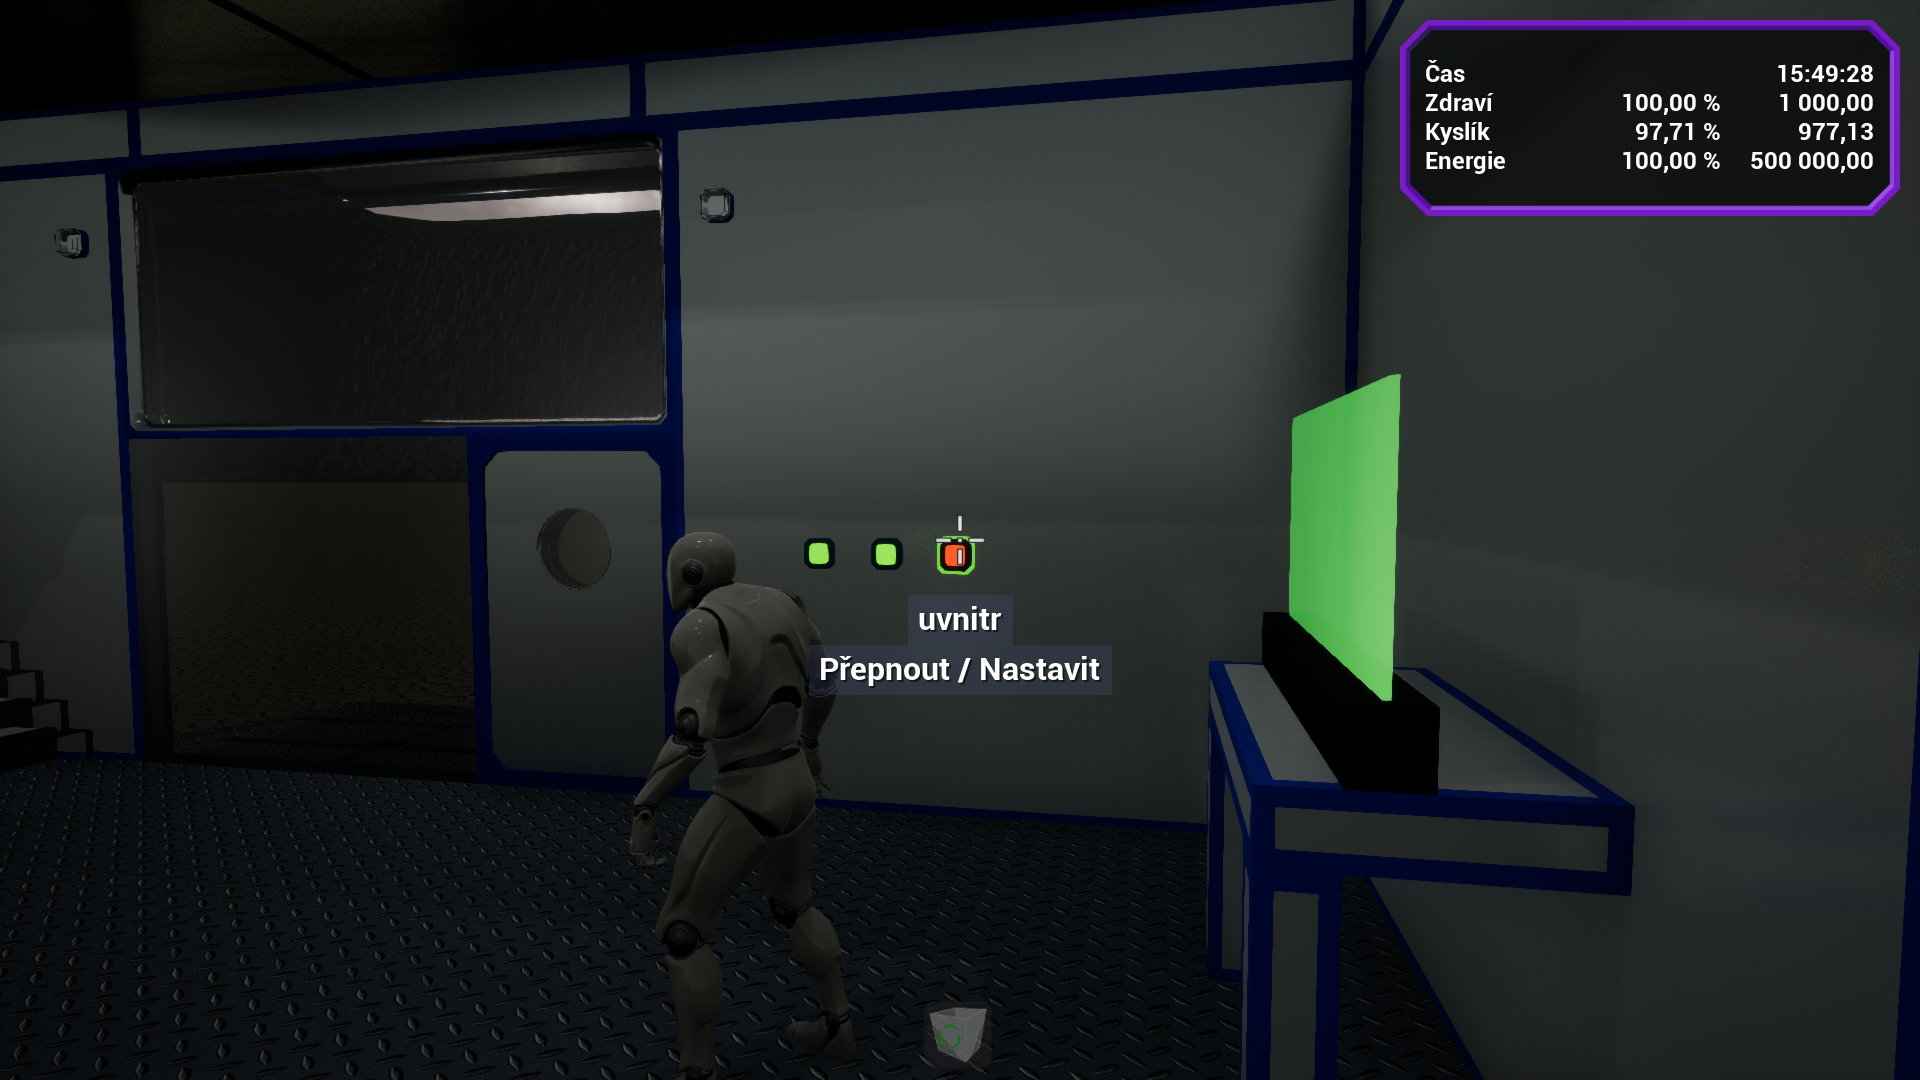
\includegraphics[ width=140mm]{../img/user/switcher/0switcherGeneral}

\caption{Přepínač - den}
\label{fig:user_switcher_0switcherGeneral}

\end{figure}

\FloatBarrier

Blok umožňuje reagovat na denní dobu - automatické přepínání na definovaný stav, pokud začne den, nebo začne noc.

V levé části le možné přiřazovat ovládané bloky

\begin{figure}[!h]\centering
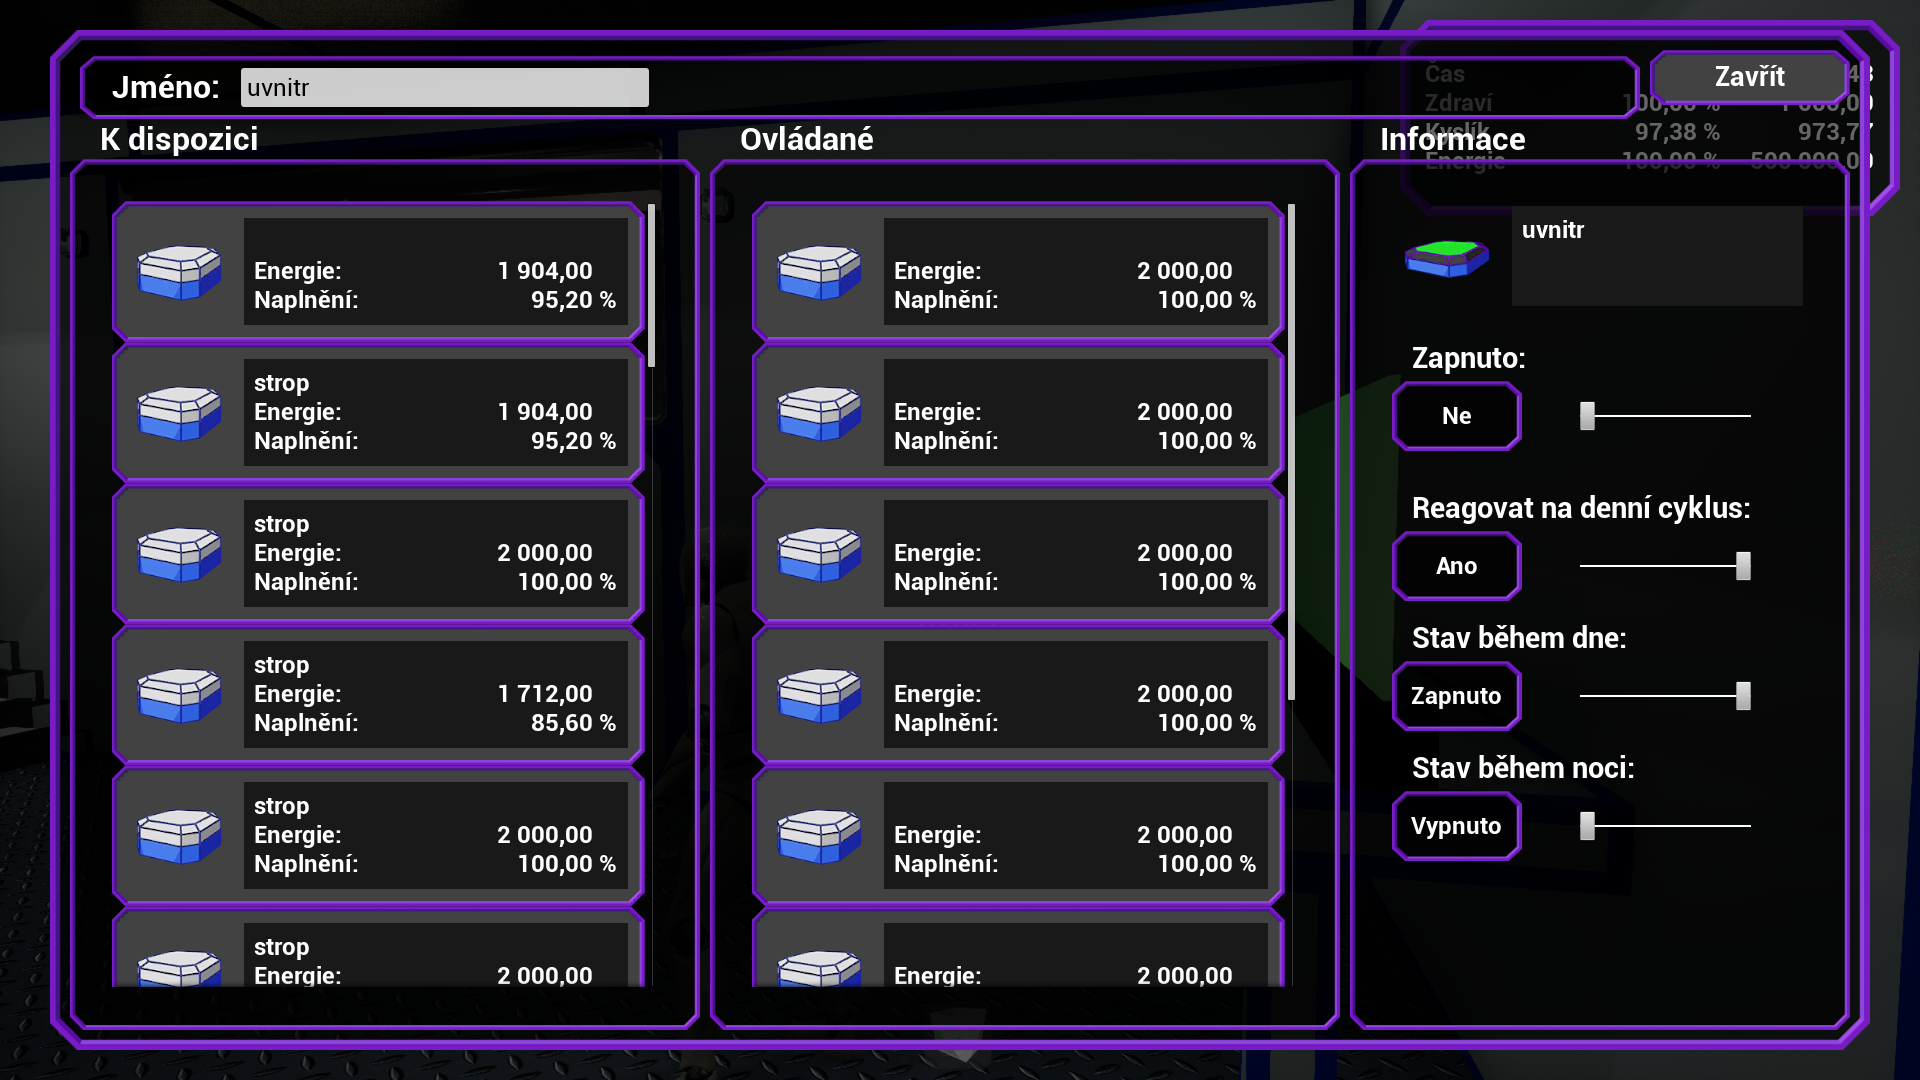
\includegraphics[ width=140mm]{../img/user/switcher/switcherControls}

\caption{Přepínač - poledne, zataženo}
\label{fig:user_switcher_switcherControls}

\end{figure}


\FloatBarrier
%!TEX root = ../prace.tex

\section{Světlo}

Světlo má podobné rozhraní jako Plnička. V levé části se přiřazuje ovladač, v pravé se edituje výkon bloku.

\begin{figure}[!ht]\centering
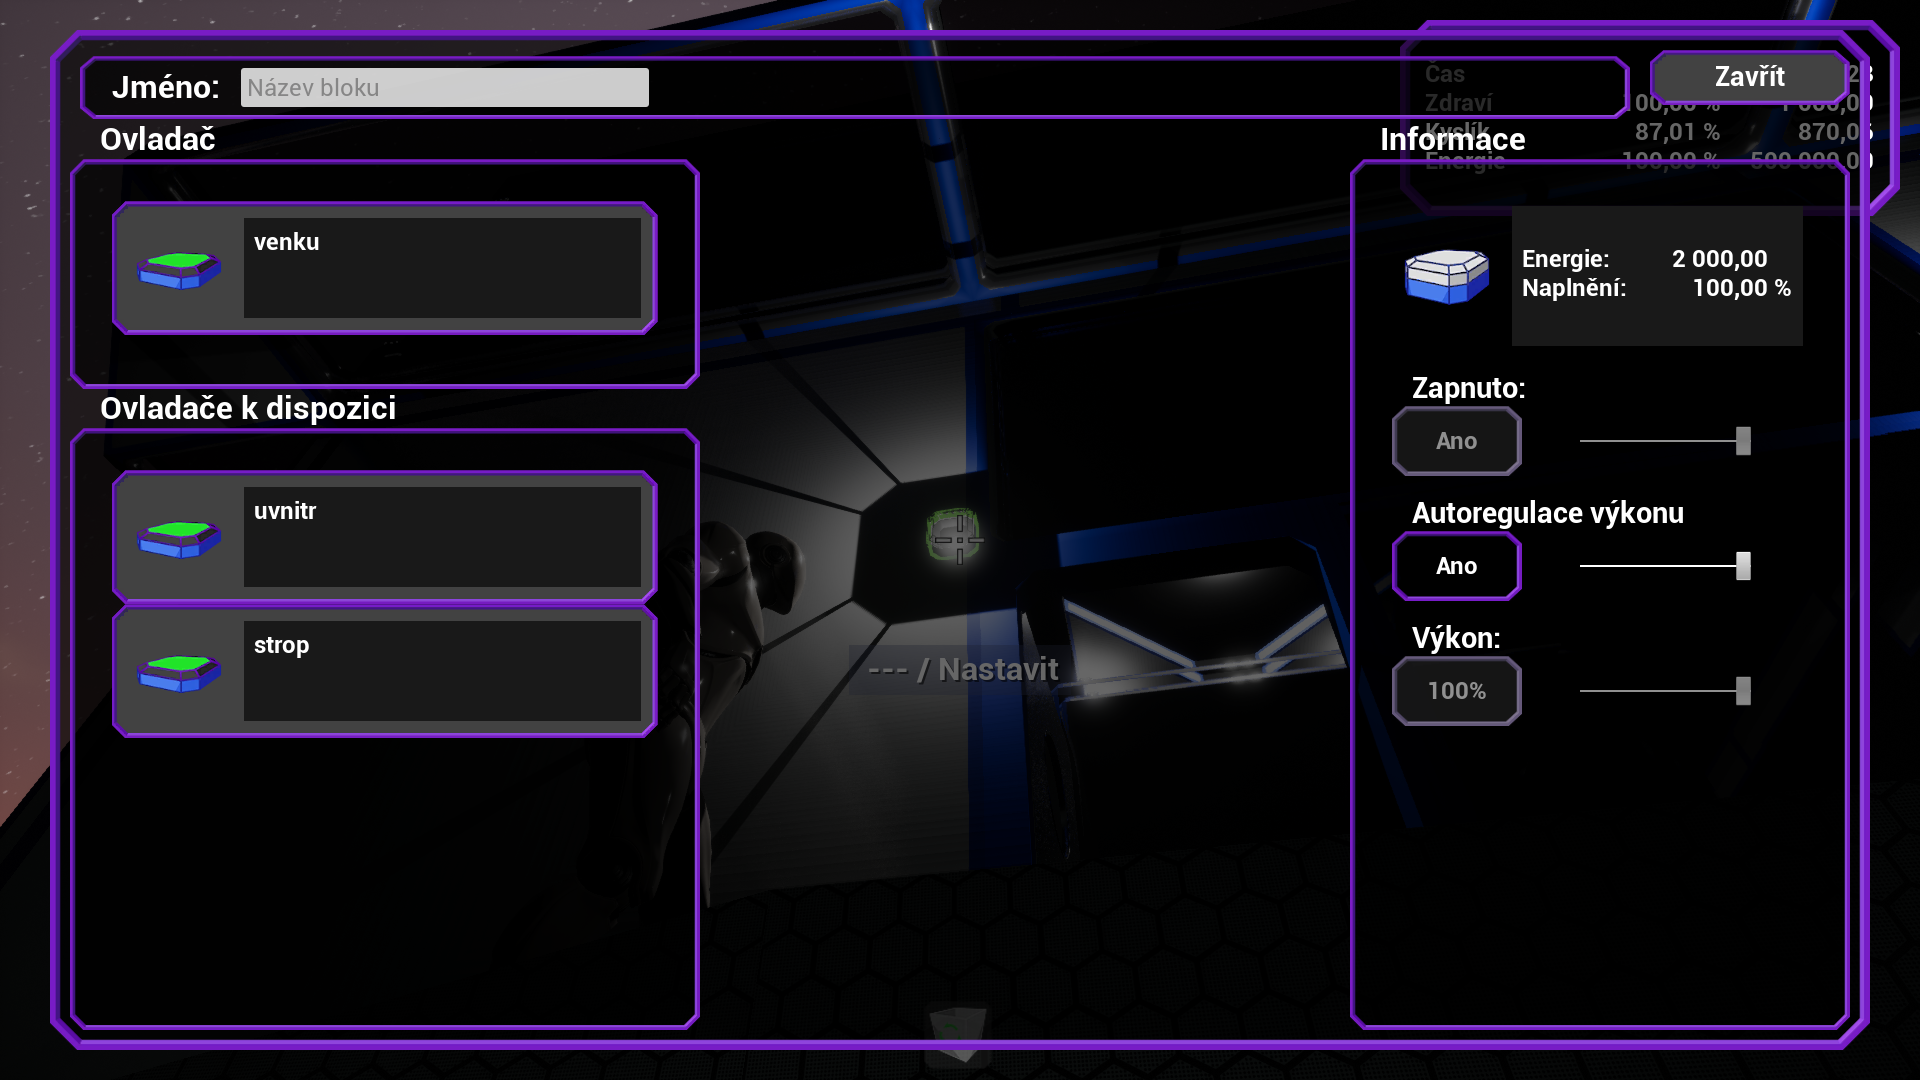
\includegraphics[ width=140mm]{../img/user/light/0light}

\caption{Světlo - ovládací obrazovka}
\label{fig:user_light_0light}

\end{figure}

\FloatBarrier

%!TEX root = ../prace.tex

\section{Kyselý déšť}

Pokud se blíží bouře kyselého deště, nebo právě jedna probíhá, hráč vidí v levé horní části obrazovky zprávu s odhadovaným časem a intenzitou.

To umožňuje strategicky řídit chod svých budov a případně limitovat spotřebovávané zdroje v případě očekávaných dlouhotrvajících bouří. Odhadovaný čas je udán v herním čase.

\begin{figure}[!ht]\centering
\includegraphics[ width=140mm]{../img/user/rain/0rainInfo}

\caption{Kyselý déšť - info}
\label{fig:user_rain_0rainInfo}

\end{figure}

\FloatBarrier

Pokud hráč není ukrytý v budově či pod nějakým blokem, dostává zásahy. Dokud má dostatek energie, je schopen odolávat účinkům bouře, v momentě, kdy mu energie dojde, začne mu ubývat zdraví.


\begin{figure}[!ht]\centering
\includegraphics[ width=140mm]{../img/user/rain/1rainDamage}

\caption{Kyselý déšť - zásahy}
\label{fig:user_rain_1rainDamage}

\end{figure}

\FloatBarrier

Pokud si hráč doplní energii, začne se mu zdraví obnovovat.

\begin{figure}[!ht]\centering
\includegraphics[ width=140mm]{../img/user/rain/2rainRefill}

\caption{Kyselý déšť - obnova zdraví}
\label{fig:user_rain_2rainRefill}

\end{figure}


\begin{figure}[!ht]\centering
\includegraphics[ width=140mm]{../img/user/rain/3rainRefill1}

\caption{Kyselý déšť - obnova zdraví}
\label{fig:user_rain_3rainRefill1}

\end{figure}

\FloatBarrier

Během bouře je též možné pozorovat animaci generátoru energie, kdy je po každém zásahu rozsvícen příslušný čtverec. Tuto animaci lze z menu vypnout a pokud má uživatel slabší stroj, tak to i doporučujeme.

\begin{figure}[!ht]\centering
\includegraphics[ width=140mm]{../img/user/rain/4rainGeneratorAnim}

\caption{Kyselý déšť - animace zásahů}
\label{fig:user_rain_4rainGeneratorAnim}

\end{figure}


\FloatBarrier



%!TEX root = ../prace.tex

\chapter{Závěr}


\section{Zhodnocení práce}


\section{Budoucí práce}


\begin{itemize}
	\item dynamičtějí mřížka? 20cm je nejspíše dost málo a vyžaduje to dost preciznosti // TODO zkusit pro test 25 či 30 cm a patřičným způsobem upravit velikosti modelů? (nejspíše to musí zůstat hardcoded, ale zkusím se nad tím zamyslet, pokud bude čas)
	\item vlastní sortování v seznamech

\end{itemize}

TODO dotazník?

%%% Seznam použité literatury
%%% Seznam použité literatury (bibliografie)
%%%
%%% Pro vytváření bibliografie používáme bibTeX. Ten zpracovává
%%% citace v textu (např. makro \cite{...}) a vyhledává k nim literaturu
%%% v souboru literatura.bib.
%%%
%%% Příkaz \bibliographystyle určuje, jakým stylem budou citovány odkazy
%%% v textu. V závorce je název zvoleného souboru .bst. Styly plainnat
%%% a unsrt jsou standardní součástí latexových distribucí. Styl czplainnat
%%% je dodáván s touto šablonou a bibTeX ho hledá v aktuálním adresáři.

\bibliographystyle{czplainnat}    %% Autor (rok) s českými spojkami
% \bibliographystyle{plainnat}    %% Autor (rok) s anglickými spojkami
% \bibliographystyle{unsrt}       %% [číslo]

\renewcommand{\bibname}{Seznam použité literatury}

%%% Vytvoření seznamu literatury. Pozor, pokud jste necitovali ani jednu
%%% položku, seznam se automaticky vynechá.

\bibliography{literatura}

%%% Kdybyste chtěli bibliografii vytvářet ručně (bez bibTeXu), lze to udělat
%%% následovně. V takovém případě se řiďte normou ISO 690 a zvyklostmi v oboru.

% \begin{thebibliography}{99}
%
% \bibitem{lamport94}
%   {\sc Lamport,} Leslie.
%   \emph{\LaTeX: A Document Preparation System}.
%   2. vydání.
%   Massachusetts: Addison Wesley, 1994.
%   ISBN 0-201-52983-1.
%
% \end{thebibliography}


%%% Obrázky v bakalářské práci
%%% (pokud jich je malé množství, obvykle není třeba seznam uvádět)
%\listoffigures

%%% Tabulky v bakalářské práci (opět nemusí být nutné uvádět)
%%% U matematických prací může být lepší přemístit seznam tabulek na začátek práce.
%\listoftables

%%% Použité zkratky v bakalářské práci (opět nemusí být nutné uvádět)
%%% U matematických prací může být lepší přemístit seznam zkratek na začátek práce.

% Soubor se všemi zkratkami uvedenými v práci

%!TEX root = prace.tex


\chapter*{Seznam použitých zkratek}
\addcontentsline{toc}{chapter}{Seznam použitých zkratek}

TODO seznam zkratek

%%% Přílohy k bakalářské práci, existují-li. Každá příloha musí být alespoň jednou
%%% odkazována z vlastního textu práce. Přílohy se číslují.
%%%
%%% Do tištěné verze se spíše hodí přílohy, které lze číst a prohlížet (dodatečné
%%% tabulky a grafy, různé textové doplňky, ukázky výstupů z počítačových programů,
%%% apod.). Do elektronické verze se hodí přílohy, které budou spíše používány
%%% v elektronické podobě než čteny (zdrojové kódy programů, datové soubory,
%%% interaktivní grafy apod.). Elektronické přílohy se nahrávají do SISu a lze
%%% je také do práce vložit na CD/DVD. Povolené formáty souborů specifikuje
%%% opatření rektora č. 23/2016.



%!TEX root = ../../prace.tex


\appendix
\chapwithtoc{Přílohy}

\renewcommand{\thesection}{\Alph{section}}

\section{Struktura souborů přílohy}
Struktura vypadá následovně:
\begin{itemize}
	\item \textit{Build} -- tato složka obsahuje výslednou zkompilovanou hru, kterou je možné spustit.
	\item \textit{Source} -- v~této složce se nachází zdrojové soubory hry.
	\item \textit{Survey} -- pod touto složkou je možné nalézt soubor dotazníku se získanými odpověďmi.
\end{itemize}



\section{Grafy k~dotazníku}
\label{sec:survey}


Níže je možné se podívat na grafy zpracované stránkou Google Forms. U~sloupcových grafů byla otázka zodpovězena na škále od 1 do 10. Krajní hodnoty, které byly v~dotazníku nabídnuty, jsou vepsány v~popisku obrázku.

\begin{figure}[!ht]\centering
\includegraphics[ width=110mm]{../img/survey/q1}
\caption{Vůbec hry nehraji -- Hraji každý den}
\label{fig:q1}
\end{figure}
\FloatBarrier


\begin{figure}[!ht]\centering
\includegraphics[ width=110mm]{../img/survey/q2}
\caption{Vůbec to neznám -- Znám je velice dobře}
\label{fig:q2}
\end{figure}
\FloatBarrier


\begin{figure}[!ht]\centering
\includegraphics[ width=110mm]{../img/survey/q3}
\caption{Velice málo (max. 1 hodinu) -- Hodně (100 a~více hodin)}
\label{fig:q3}
\end{figure}
\FloatBarrier


\begin{figure}[!ht]\centering
\includegraphics[ width=110mm]{../img/survey/q4}
\caption{Otázka 4}
\label{fig:q4}
\end{figure}
\FloatBarrier


\begin{figure}[!ht]\centering
\includegraphics[ width=110mm]{../img/survey/q5}
\caption{Příliš malé -- Dostatečně velké}
\label{fig:q5}
\end{figure}
\FloatBarrier


\begin{figure}[!ht]\centering
\includegraphics[ width=110mm]{../img/survey/q6}
\caption{Stavění bylo oproti jiným hrám nepříjemné -- Stavění mě oproti jiným hrám opravdu bavilo}
\label{fig:q6}
\end{figure}
\FloatBarrier


\begin{figure}[!ht]\centering
\includegraphics[ width=110mm]{../img/survey/q7}
\caption{Velice nepovedená, nikdy se k~ní nevrátím -- Zdařilá, rád/a bych si v~budoucnu dokončenou hru zahrál/a}
\label{fig:q7}
\end{figure}
\FloatBarrier


\newpage

\section{Struktura souboru uložené hry}
\label{sec:saveGame}

TODO

Základní struktura binárního souboru uložené hry je níže. Datové typy odpovídají datovým typům \UEu{} a~vlastním definovaným typům. Ty popíšeme v~následujících tabulkách. Vzhledem k~použití dědičnosti u~některých vlastních datových typů musíme přistoupit k~zápisu \TT{[název datového typu předka]} bez uvedení názvu vlastnosti. Tím dáváme najevo fakt, že daná struktura navíc obsahuje na dané pozici všechny datové položky daného předka. Dále u~některých vlastností využíváme podmínek. Pokud taková podmínka není splněna, data se v~binárním souboru vůbec neobjeví.

\begin{code}
FString                                     SaveName
FDateTime                                   SavedDate
FTimespan                                   PlayedTime
bool                                        IsQuickSave
uint8                                       MinBoxSize
float                                       CurrentTime
FVector                                     PlayerPosition
FRotator                                    PlayerRotation
FRotator                                    PlayerCameraRotation
bool                                        PlayerUseFPSCamera
TArray<FBlockInfo>                          usedBlocks
TArray<FInventoryBuildableBlockInfo>        buildableBlocks
TArray<FInventoryBuildableItemBlockInfo>    inventoryBuildableBlocks
FInventoryTags                              inventoryTags
int32                                       InventoryCurrentIndex
FOxygenComponentInfo                        PlayerOxygenComponent
FElectricityComponentInfo                   PlayerElectricityComponent
float                                       PlayerHealth
bool                                        IsCreativeMode
FWeatherState                               weatherState
\end{code}



\subsubsection{FBlockInfo}

\begin{code}
[FBlockBaseInfo]
FVector                                     Location
FRotator                                    Rotation
float                                       Health
TMap<FString, FString>                      BlockSpecificData
bool                                        HasRelationshipData
if (HasRelationshipData)
    FBlockWithRelationshipInfo              RelationshipInfo
\end{code}

\newpage


\subsubsection{FBlockWithRelationshipInfo}
\begin{code}
FGuid                                       ID
TArray<FRelationshipInfo>                   Relationships
\end{code}

\subsubsection{FRelationshipInfo}
\begin{code}
FGuid                                       TargetID
uint8                                       RelationshipType
\end{code}


\subsubsection{FBlockBaseInfo}
\begin{code}
int32                                       ID
FVector                                     Scale
FString                                     Name
TMap<FString, int32>                        AdditionalFlags
bool                                        HasOxygenData
if (HasOxygenData)
    FOxygenComponentInfo                    OxygenInfo
bool                                        HasElectricityData
if (HasElectricityData)
    FElectricityComponentInfo               ElectricityInfo
\end{code}





\subsubsection{FOxygenComponentInfo}
\begin{code}
float                                       CurrentObjectOxygen
\end{code}


\subsubsection{FElectricityComponentInfo}
\begin{code}
float                                       CurrentObjectEnergy
bool                                        HasPoweredBlockInfo
if (HasPoweredBlockInfo)
    FPoweredBlockInfo                       PoweredBlockInfo
\end{code}

\subsubsection{FPoweredBlockInfo}
\begin{code}
bool                                        IsOn
bool                                        AutoregulatePower
float                                       PowerConsumptionPercent
\end{code}



\subsubsection{FInventoryBuildableBlockInfo, FInventoryBuildableItemBlockInfo}
\begin{code}
TArray<FString>                             Tags
\end{code}

\newpage


\subsubsection{FInventoryTags}
\begin{code}
int32                                       CurrentActiveIndex
TArray<FInventoryTagGroup>                  InventoryGroupList
\end{code}

\subsubsection{FInventoryTagGroup}
\begin{code}
FString                                     GroupName
bool                                        IsGroupEnabled
uint8                                       GroupType
TArray<FTagGroup>                           GroupList
\end{code}

\subsubsection{FTagGroup}
\begin{code}
FString                                     GroupName
TArray<FString>                             Tags
bool                                        LetVisibleAll
\end{code}

\subsubsection{FWeatherState}
\begin{code}
int32                                       CurrentDefinitionID
bool                                        IsInWeatherChange
bool                                        ApplyDamage
float                                       CurrentWaitingTime
float                                       TargetWaitingTime
float                                       BaseWeatherIntensity
float                                       CurrentWeatherIntensity
float                                       TargetWeatherIntensity
float                                       BaseCloudOpacity
float                                       CurrentCloudOpacity
float                                       TargetCloudOpacity
float                                       HitpointsCounter
float                                       PlayerHitpointCounter
float                                       EaseIn
float                                       EaseOut
uint8                                       StormState
\end{code}

\openright
\end{document}
